\documentclass[twocolumn,aps,pra,showpacs,superscriptaddress,nofootinbib]{revtex4-1}

\usepackage[caption=false]{subfig}
\usepackage{amsfonts}
\usepackage{filecontents}
\usepackage{graphicx}
\usepackage{lipsum}
\usepackage{mathtools}
\usepackage{microtype}
\usepackage{paralist}
\usepackage{pgfplots}
\usepackage{physics}
\usepackage{siunitx}

\usepackage{hyperref}
\usepackage{cleveref}

\newcommand{\qd}{quantum dot}
\newcommand{\qds}{quantum dots}

\newcommand{\Qd}{Quantum dot}
\newcommand{\Qds}{Quantum dots}


\pgfplotsset{compat=1.4}

\usepgfplotslibrary{external}
\usepgfplotslibrary{colorbrewer}
\usetikzlibrary{pgfplots.groupplots}

\begin{document}

\title{Collective Rabi dynamics of electromagnetically-coupled quantum dot ensembles}

\author{Connor Glosser}
\email[Corresponding author; ]{glosser1@msu.edu}
\affiliation{Department of Physics \& Astronomy, Michigan State University\\567 Wilson Road, East Lansing MI 48824 USA}
\affiliation{Department of Electrical \& Computer Engineering, Michigan State University\\428 South Shaw Lane, East Lansing MI 48824, USA}

\author{B.\ Shanker}
\affiliation{Department of Electrical \& Computer Engineering, Michigan State University\\428 South Shaw Lane, East Lansing MI 48824, USA}

\author{Carlo Piermarocchi}
\email[ ]{piermaro@msu.edu}
\affiliation{Department of Physics \& Astronomy, Michigan State University\\567 Wilson Road, East Lansing MI 48824 USA}


\date{\today}
\pacs{1.1}

\begin{abstract}
  Rabi oscillations typify the inherent nonlinearity of optical excitations in \qds{}, and, in contrast to atoms, ensembles of \qds{} realize spatial configurations characterized by quenched randomness.
Using a highly efficient integral equation formulation to solve the 3D Maxwell-Bloch equations in ensembles of up to $10^4$ quantum dots, we observe features in the collective dynamics due to the interplay of nonlinearity, non-equilibrium excitation, and electromagnetic coupling between the dots.
The approach allows us to observe the dynamics of each dot in the ensemble without resorting to spatial averages.
Our simulations predict synchronized multiplets of dots that exchange energy, dots that dynamically couple to screen the effect of incident external radiation, as well as localization of the polarization due to randomness and interactions. These results suggest new experimental strategies for isolating light-induced  dynamical quantum dot molecules in dot ensembles.

\end{abstract}

\maketitle

\section{\label{sec:introduction}Introduction}
Semiconductor structures containing a large number of quantum dots offer ideal environments for exploring light-matter interactions in regimes where non-equilibrium, non-linearity, and randomness lead to new phenomena.
Optical excitations (excitons) give rise to characteristic Rabi oscillations in \qds{} that mimic two-level atoms.
Time-resolved~\cite{stievater,shih} and spectral~\cite{kamada} methods have revealed Rabi oscillations in many such systems.
In these experiments, the excitation typically involves a large collection of dots while an optical mask isolates the signal from a single dot.
\Qds{} have stronger dipolar transitions than atoms and their light-induced oscillations generate strong secondary fields that depend on random spatial configurations.
We therefore expect, at least in some regions of the sample, these secondary fields to produce modified collective behavior in the exciton dynamics.
Signatures of collective effects due to long-range electromagnetic coupling have arisen in the photoluminescence emissions of ensembles of \qds{}~\cite{forchel}.

Here, we develop a computational framework to discover signatures of collective effects in strongly-driven quantum dots with a microscopic formalism.
Current solution strategies for Maxwell-Bloch systems either resort to a continuum treatment of macroscopic fields~\cite{} or mesh-based strategies (such as finite-difference time-domain method )~\cite{Vanneste2001, Fratalocchi2008} for full-wave models of the simulation domain---techniques undermined by their computational overhead and numerical sensitivities~\cite{Baczewski2013}.
In this paper, we develop integral equation based approach that facilitates fast and accurate field calculations by allowing direct communication of field quantities between \qds{}. This provides three salient advantages: (i) there is need for a computational grid to propagate fields, and as a result, there is no numerical dispersion, (ii) the radiation/Sommenfeld radiation condition is explicitly included in the Green's function, and (iii) both near and far fields are modeled to high accuracy unlike differential equation methods that rely on an underlying grid. \textcolor{red}{
Moreover, a highly-tuned predictor-corrector scheme provides an accurate account of the propagation and phase effects between \qds{}, even for very close particles.THIS IS VERY ODD; people do not know as yet what the challenges are and why are proposing what we are doing} 

We find that in some instances the Rabi oscillation of a set of strongly coupled dots features additional oscillations due to an exchange of energy between the dot or dynamical creation of dark multiplets that completely screen the dots from Rabi rotation.


....Anything else we can mention?

\section{\label{section:problem statement}Problem Statement}
We wish to consider the evolution of a \qd{} in response to an externally produced electric field.
If we concern ourselves only with electric dipole transitions in a two-level system, we may write the time-dependence of the dot's quantum state as
\begin{equation}
  i \hbar \dv{\hat{\rho}}{t} = \commutator{\hat{\mathcal{H}}(t)}{\hat{\rho}} - \hat{\mathcal{D}}\qty[\hat{\rho}].
  \label{eq:liouville}
\end{equation}
Here, $\hat{\mathcal{H}}(t)$ represents a local Hamiltonian that governs the internal two-level structure of the \qd{} as well as its interaction with an electromagnetic field while $\hat{\mathcal{D}}$ provides dissipation terms that account for emission effects phenomenologically.
Formally,
\begin{subequations}
  \begin{align}
    \hat{\mathcal{H}}(t) &\equiv \mqty(0 & \hbar \chi(t) \\ \hbar \chi^*(t) & \hbar \omega_0) \label{eq:hamiltonian}\\
    \hat{\mathcal{D}}\qty[\hat{\rho}] &\equiv \mqty( \qty(\rho_{00} - 1)/{T_1} & \rho_{01}/{T_2} \\ \rho_{10}/{T_2} & \rho_{11}/T_1 ) \label{eq:dissipator}
  \end{align}
\end{subequations}
where \todo{Expression tree; bad form?}$\chi(t) \equiv \vb{d} \cdot \vb{E}(\vb{r}, t)/\hbar$, $\vb{d} \equiv \matrixel{1}{e \hat{\vb{r}}}{0}$, and $\ket{0}$ \& $\ket{1}$ represent the highest valence and lowest conduction states of the \qd{}.
Finally, the $T_1$ and $T_2$ constants represent phenomenalogical emission and relaxation times~\cite{}.
Assuming $c/\omega_0 \gg \sqrt{\expval{\hat{\vb{r}}^2}}$, we may neglect the spatial variation in $\vb{E}(\vb{r}, t)$ in calculating $\chi(t)$ and thereby consider each \qd{} as a localized point in space.

As $\expval{\hat{A}} = \Tr[\hat{\rho}\hat{A}]$ yields the expectation value of an operator $\hat{A}$ in a density matrix formulation, the evolution of \cref{eq:liouville} for a \qd{} located at $\vb{r}_j$ gives rise to a classical polarization $\vb{P} = \expval{\hat{\vb{P}}}$ that produces additional radiation through secondary emission effects.
Writing this polarization as
\begin{equation}
  \begin{aligned}
    \vb{P}(\vb{r}, t) &= \Tr[\hat{\rho} \cdot \hat{\vb{d}}] \delta(\vb{r} - \vb{r}_j) \\
                      &= 2 \Re[\rho_{01}\vb{d}]\delta(\vb{r} - \vb{r}_j),
  \end{aligned}
\end{equation}
we may compute the total electric field at any point through the dyadic electric field Green's function\cite{Rothwell2008}
\begin{widetext}
  \begin{equation}
    \vb{E}(\vb{r}, t) \equiv \vb{E}_0(\vb{r}, t) - \frac{1}{4\pi\varepsilon} \int
      \qty(I - \bar{\vb{r}} \bar{\vb{r}}) \frac{\ddot{\vb{P}}(\vb{r}', t_R)}{c^2\abs{\vb{r} - \vb{r}'}} +
      \qty(I - 3\bar{\vb{r}} \bar{\vb{r}}) \frac{\dot{\vb{P}}(\vb{r}', t_R)}{c\abs{\vb{r} - \vb{r}'}^2} +
      \qty(I - 3\bar{\vb{r}} \bar{\vb{r}}) \frac{\vb{P}(\vb{r}', t_R)}{\abs{\vb{r} - \vb{r}'}^3}
    \dd[3]{\vb{r}'}
    \label{eq:total field}
  \end{equation}
\end{widetext}
where $\bar{\vb{r}} = \vb{r} - \vb{r}'/\abs{\vb{r} - \vb{r}'}$ and $t_R = t - \abs{\bar{\vb{r}}}/c$.
In a system composed of multiple dots, the additional convolution appearing in \cref{eq:total field} serves to couple the the evolution of \cref{eq:liouville} for each \qd{} by way of the off-diagonal matrix elements in \cref{eq:hamiltonian}.

\section{Computational approach}
The computational approach is based on...
\begin{figure}
  \centering
  \input{figures/frame_comparison.tex}
  \caption{\label{fig:frame comparison}
    Validity of the rotating-frame approximation within an integral equation framework.
    The fixed- and rotating-frame populations for a collection of quantum dots display nearly identical trajectories.
  }
\end{figure}

\section{\label{section:results}Numerical Results}
\begin{table}
  \begin{ruledtabular}
    \begin{tabular}{lll}
      Quantity                 & Symbol            & Value                        \\ \hline
      Speed of light           & $c$               & \SI{300}{\micro\meter \per \pico\second} \\
      Transition frequency     & $\omega_0$        & $\SI{1500}{\milli\eV}/\hbar$ \\
      Transition dipole moment & $\vb{d}$          & \SI{10}{\elementarycharge\bohr} (uniform) \\
      Relaxation times         & $T_{1}, T_{2}$    & \SIlist{10;20}{\pico\second} \\
      Laser frequency          & $\omega_L$        & $\SI{1500}{\milli\eV}/\hbar$ \\
      Laser wavevector         & $\vb{k}_L$        & $\omega_L/c$ ($\vb{k}_L \cdot \vb{d} = 0$) \\
      Pulse width              & $\sigma/\omega_L$ & \SI{1}{\pico\second} \\
      %Number density          & $n$               & $< \SI{1.6e4}{\micro\meter\tothe{-3}}$ \\
      %\hline
      %Speed of light           & $c$            & \SI{299.792458}{\micro\meter\per\pico\second} \\
      %Reduced Planck constant  & $\hbar$        & \SI{0.65821193}{\milli\eV \pico\second} \\
      %Vacuum permeability      & $\mu_0$        & \SI{2.013e-4}{\milli\eV \pico\second\squared \per \elementarycharge \per \micro\meter}
    \end{tabular}
  \end{ruledtabular}
  \caption{\label{table:parameters}Simulation parameters; \si{\elementarycharge} and \si{\bohr} denote the elementary charge and Bohr radius.}
\end{table}

Here we detail the results of investigations into coupled \qd{} behavior with the model presented thus far.
Our algorithm reliably handles tens of thousands of \qds{} and can simulate ten picoseconds of system dynamics in two days on a single processor.
We perform simulations of systems of \qds{} randomly distributed throughout a simulation volume experiencing a laser pulse of the form
\begin{equation}
  \tilde{\mathbf{E}}_L(\vb{r}, t) = \tilde{\mathbf{E}}_0 e^{-(\vb{k}_L \cdot \vb{r} - \omega_L t)^2/(2\sigma^2)}.
  \label{eq:pulse envelope}
\end{equation}
\Cref{table:parameters} provides the physical system parameters unless otherwise stated.

\begin{figure}
  \begin{filecontents}{high_density_stats.dat}
time     ubound               lbound              p1                 p2                 p3                 p4                  p5                 p6                 p7                 p8                  p9                 p10                p11                p12                p13                p14                p15                 p16                 p17                 p18                p19                 p20                 p21                 p22                p23                 p24                 p25                p26                 p27                p28                 p29                p30                p31                p32                 p33                p34                p35                 p36                 p37                p38                p39                p40                 p41                p42                p43                p44
0.       1.                   1.                  1.                 1.                 1.                 1.                  1.                 1.                 1.                 1.                  1.                 1.                 1.                 1.                 1.                 1.                 1.                  1.                  1.                  1.                 1.                  1.                  1.                  1.                 1.                  1.                  1.                 1.                  1.                 1.                  1.                 1.                 1.                 1.                  1.                 1.                 1.                  1.                  1.                 1.                 1.                 1.                  1.                 1.                 1.                 1.
0.15625  0.9999999999996378   0.999999999999718   0.9999999999997039 0.9999999999997039 0.9999999999997039 0.9999999999997039  0.9999999999997039 1.                 0.9999999999997    0.9999999999997039  0.9999999999997039 0.9999999999997039 0.9999999999998039 0.9999999999997039 0.9999999999997039 0.9999999999997039 0.9999999999996766  0.9999999999996766  0.9999999999997039  0.9999999999997039 0.9999999999995945  0.9999999999996766  0.9999999999997039  0.9999999999997039 0.9999999999996766  0.9999999999997039  0.9999999999997039 0.9999999999996766  0.9999999999997039 0.9999999999997039  0.9999999999998    0.9999999999997039 0.9999999999997039 0.9999999999996766  0.9999999999997039 0.9999999999997039 0.9999999999997039  0.9999999999996766  0.9999999999997039 0.9999999999997039 0.9999999999997039 0.9999999999996766  0.9999999999997039 0.9999999999997039 0.9999999999997039 0.9999999999996766
0.3125   0.9999999999967255   0.9999999999972855  0.9999999999971938 0.9999999999970001 0.9999999999971    0.9999999999970001  0.9999999999973063 0.9999999999999    0.9999999999983    0.9999999999970001  0.9999999999971    0.9999999999972    0.9999999999993062 0.9999999999975437 0.9999999999971062 0.99999999999735   0.9999999999970001  0.9999999999968     0.9999999999969937  0.9999999999971501 0.9999999999959562  0.99999999999695    0.9999999999970001  0.9999999999972062 0.9999999999968999  0.9999999999970499  0.9999999999969937 0.9999999999968999  0.99999999999735   0.9999999999970001  0.9999999999992    0.9999999999971062 0.9999999999970938 0.9999999999970001  0.9999999999971501 0.9999999999971    0.9999999999969937  0.9999999999970001  0.9999999999975437 0.9999999999970938 0.9999999999975563 0.9999999999968999  0.9999999999972    0.9999999999970938 0.9999999999973    0.9999999999970001
0.46875  0.9999999999808656   0.9999999999843944  0.999999999985175  0.9999999999831289 0.9999999999839    0.9999999999831289  0.999999999985875  0.9999999999995    0.9999999999940515 0.999999999982829   0.9999999999839    0.999999999985275  0.999999999998025  0.999999999988825  0.9999999999836234 0.9999999999868555 0.999999999982829   0.999999999981232   0.9999999999830289  0.9999999999844039 0.9999999999758055  0.9999999999822304  0.9999999999832055  0.9999999999848984 0.9999999999821524  0.9999999999833289  0.9999999999834055 0.9999999999822304  0.9999999999867555 0.999999999982925   0.9999999999978288 0.9999999999836054 0.9999999999843765 0.9999999999828251  0.9999999999844039 0.9999999999839    0.9999999999833055  0.9999999999828251  0.999999999988625  0.9999999999840999 0.9999999999885523 0.999999999982225   0.999999999985275  0.9999999999842094 0.9999999999860789 0.9999999999830289
0.625    0.999999999908596    0.9999999999258837  0.9999999999343    0.9999999999218    0.9999999999261    0.9999999999207     0.9999999999398    0.9999999999982    0.9999999999745    0.9999999999185     0.9999999999262    0.9999999999359    0.9999999999896    0.999999999957     0.9999999999246    0.9999999999455    0.9999999999187     0.9999999999081     0.9999999999199     0.9999999999296    0.9999999998857     0.9999999999145     0.9999999999211     0.9999999999334    0.9999999999144     0.9999999999222     0.999999999923     0.9999999999146     0.999999999945     0.9999999999198     0.9999999999912    0.999999999924     0.99999999993      0.9999999999193     0.9999999999295    0.9999999999261    0.9999999999221     0.9999999999193     0.9999999999558    0.9999999999277    0.9999999999555    0.999999999915      0.999999999936     0.9999999999278    0.9999999999406    0.9999999999203
0.78125  0.9999999996062331   0.999999999682793   0.9999999997345218 0.9999999996728851 0.9999999996924008 0.9999999996631351  0.9999999997641874 0.9999999999937249 0.9999999998902883 0.9999999996511656  0.9999999996931024 0.9999999997453626 0.9999999999614344 0.9999999998413492 0.9999999996856117 0.9999999997915087 0.9999999996531141  0.9999999995976     0.9999999996584656  0.9999999997118507 0.9999999995090422  0.999999999629818   0.9999999996664891  0.9999999997320203 0.9999999996306156  0.9999999996715313  0.9999999996776078 0.9999999996309157  0.9999999997894055 0.9999999996594852  0.9999999999619024 0.9999999996819797 0.9999999997163258 0.9999999996570602  0.9999999997114507 0.9999999996925008 0.9999999996720367  0.9999999996575836  0.9999999998366266 0.9999999997014297 0.9999999998353032 0.9999999996334461  0.9999999997456719 0.9999999997021313 0.9999999997681414 0.9999999996624351
0.9375   0.999999998423238    0.9999999987352037  0.9999999989906563 0.9999999987220313 0.9999999988035625 0.999999998665      0.9999999991224375 0.999999999978     0.9999999995845312 0.9999999986101625  0.9999999988072125 0.9999999990438062 0.999999999864825  0.9999999994213188 0.9999999987745625 0.9999999992340001 0.9999999986208062  0.9999999983684813  0.9999999986432062  0.9999999988942937 0.9999999980236     0.9999999985111375  0.9999999986848437  0.9999999989852687 0.9999999985182437  0.9999999987070437  0.999999998739225  0.9999999985183375  0.9999999992258625 0.9999999986532     0.9999999998615687 0.999999998757325  0.9999999989193376 0.9999999986427562  0.9999999988926938 0.9999999988045125 0.9999999987114875  0.9999999986464     0.9999999994049688 0.9999999988461062 0.999999999399775  0.9999999985303375  0.99999999904465   0.99999999884905   0.999999999138075  0.9999999986671437
1.09375  0.9999999940489793   0.9999999952373225  0.9999999963479899 0.9999999952728461 0.9999999955910476 0.9999999950002493  0.999999996861832  0.9999999999240594 0.9999999985257406 0.9999999947739383  0.9999999956068907 0.9999999965637523 0.9999999995107961 0.999999997934232  0.9999999954773625 0.9999999972779687 0.9999999948234539  0.9999999937785585  0.999999994911714   0.9999999959677766 0.9999999925190461  0.9999999943572149  0.9999999950989266  0.9999999963351898 0.9999999943956344  0.9999999951888188  0.9999999953337406 0.9999999943929788  0.9999999972475742 0.9999999949677757  0.9999999995313711 0.9999999954028297 0.9999999960787039 0.9999999949264117  0.9999999959613516 0.9999999955957977 0.9999999952134094  0.9999999949448812  0.9999999978805375 0.9999999957691601 0.9999999978612594 0.9999999944445     0.999999996567204  0.9999999957811352 0.9999999969209227 0.9999999950272148
1.25     0.9999999786802626   0.9999999829748861  0.9999999873838    0.9999999833523    0.9999999845301    0.9999999822076     0.9999999892247    0.999999999747     0.9999999949316    0.999999981339      0.999999984591     0.9999999881671    0.9999999983789    0.999999992916     0.9999999841106    0.9999999906873    0.999999981548      0.9999999775189     0.9999999818755     0.999999985967     0.9999999731747     0.9999999797126     0.9999999826382     0.9999999873396    0.999999979885      0.9999999829849     0.999999983565     0.9999999798681     0.9999999905796    0.9999999821315     0.9999999984377    0.9999999838146    0.9999999863999    0.9999999819772     0.9999999859431    0.9999999845483    0.9999999830925     0.9999999820592     0.9999999927398    0.9999999852132    0.9999999926722    0.9999999800699     0.9999999881793    0.9999999852584    0.9999999894365    0.9999999823664
1.40625  0.9999999272801493   0.9999999420531726  0.9999999583800921 0.9999999440757765 0.9999999482292625 0.9999999396845961  0.9999999645885219 0.9999999991969437 0.9999999833515648 0.9999999365395383  0.9999999484414039 0.9999999610146008 0.9999999948925906 0.9999999768946609 0.9999999467628617 0.9999999695068227 0.9999999373624227  0.9999999227155422  0.9999999385123649  0.9999999533561945 0.9999999083548656  0.9999999305766102  0.9999999413922899  0.9999999581800172 0.9999999312669758  0.9999999426746101  0.9999999448047523 0.9999999311941125  0.9999999691427407 0.9999999395456657  0.9999999950124602 0.999999945659132  0.9999999549106234 0.9999999390013922  0.9999999532718813 0.9999999482873766 0.9999999430834844  0.999999939334011   0.9999999763189898 0.9999999506743242 0.9999999760925391 0.999999931930725   0.9999999610560695 0.999999950835007  0.9999999653116531 0.9999999404196835
1.5625   0.9999997634759841   0.9999998119244535  0.9999998689657188 0.9999998207125438 0.9999998346763562 0.9999998050000437  0.9999998889140375 0.999999997580625  0.9999999481302437 0.9999997941730124  0.9999998353618937 0.9999998773388    0.9999999844830187 0.9999999284762    0.9999998298017875 0.9999999047928312 0.9999997972325875  0.99999974670155    0.9999998010659312  0.9999998519766813 0.9999997013328125  0.999999773481125   0.9999998112777063  0.9999998680630124 0.9999997760322625  0.9999998158279187  0.9999998231252875 0.9999997757701999  0.9999999036197187 0.999999804888725   0.999999984990125  0.999999825908525  0.9999998572278562 0.9999998030604937  0.9999998516934812 0.9999998348345438 0.9999998172321375  0.9999998043226312  0.9999999266520312 0.9999998429381125 0.9999999259311437 0.99999977830205    0.9999998774733813 0.9999998434819063 0.9999998912685    0.9999998079674938
1.71875  0.9999992657481732   0.9999994174512327  0.9999996065449336 0.9999994514443328 0.9999994962034805 0.9999993983788297  0.9999996678671633 0.9999999930746586 0.9999998459338445 0.9999993628208742  0.9999994982865539 0.9999996319167062 0.9999999554066086 0.9999997896366117 0.9999994807545695 0.9999997169954757 0.9999993736108758  0.9999992075762125  0.9999993857780687  0.9999995517237132 0.9999990713779602  0.9999992945577485  0.9999994200338539  0.9999996028288617 0.9999993033950507  0.9999994355147562  0.999999459068825  0.9999993025543196  0.9999997133964711 0.999999398982075   0.9999999570560243 0.9999994677135234 0.9999995685945571 0.999999393109743   0.9999995508170203 0.9999994965676352 0.9999994399548563  0.9999993976388547  0.9999997841455351 0.9999995227209023 0.9999997819652711 0.9999993108050593  0.9999996323329914 0.9999995244753351 0.9999996751732155 0.9999994092829789
1.875    0.9999978233778156   0.9999982770413197  0.9999988738026    0.9999983982857    0.999998535068     0.9999982280059     0.9999990541758    0.9999999811351    0.9999995625785    0.9999981164355     0.9999985410672    0.9999989472875    0.999999878003     0.9999994113166    0.9999984883253    0.9999991994019    0.9999981526095     0.9999976319912     0.9999981894575     0.9999987049912    0.9999972435867     0.9999979017648     0.9999982986505     0.9999988598901    0.999997930696      0.9999983490993     0.9999984211316    0.999997928221      0.9999991888973    0.9999982324651     0.9999998826198    0.9999984467653    0.9999987567554    0.9999982143835     0.9999987022235    0.9999985357246    0.9999983621354     0.9999982298375     0.9999993957231    0.9999986161859    0.999999389454     0.999997953812      0.9999989485135    0.9999986215845    0.9999990757678    0.9999982652555
2.03125  0.999993836122056    0.9999951322172571  0.9999969282002235 0.9999955370652742 0.9999959356040649 0.9999950159765015  0.9999974351365031 0.9999999510493156 0.9999988142950055 0.999994681347136   0.9999959520425946 0.9999971314968742 0.9999996814030625 0.9999984313948961 0.9999958004869187 0.999997844361943  0.9999947967673016  0.9999932372244649  0.9999949034195305  0.9999964321703532 0.9999921843616578  0.9999940367740844  0.9999952350187461  0.9999968802203101 0.9999941266736969  0.9999953923837586  0.9999956017241289 0.9999941199092922  0.9999978151984492 0.9999950362631336  0.9999996943350171 0.9999956743551867 0.999996584011818  0.9999949828042212  0.9999964241123344 0.9999959361996297 0.9999954280013149  0.9999950330895672  0.9999983895668235 0.9999961724840414 0.9999983724203062 0.9999941956101766  0.9999971349335031 0.9999961883364539 0.9999974958872687 0.9999951356743446
2.1875   0.9999833196842388   0.9999868588532511  0.9999920177186813 0.9999881336051625 0.9999892408436063 0.9999866096947563  0.9999933768817563 0.9999998789777063 0.9999969324332687 0.9999856501841937  0.9999892838023188 0.9999925539548937 0.9999992088165375 0.9999960196330687 0.9999888675262063 0.9999944747355    0.9999860009937626  0.999981534978      0.9999862963893374  0.9999906269787563 0.9999788252121375  0.9999838003529687  0.99998725728185    0.999991863540975  0.9999840661449563  0.9999877269975626  0.9999883060202562 0.9999840489128813  0.9999943977309188 0.9999866867971188  0.9999992429329875 0.9999885027824125 0.9999910526761188 0.9999865348807813  0.9999906046044625 0.9999892389675438 0.9999878173123374  0.9999866911468375  0.9999959132677563 0.999989901650175  0.999995868652275  0.9999842627100249  0.999992563119625  0.9999899460782188 0.9999935395678875 0.9999869740320124
2.34375  0.9999568514123776   0.9999660913953254  0.9999802421425906 0.9999698919570587 0.9999728253504883 0.9999656279495711  0.9999837141491063 0.9999997149504485 0.999992418355907  0.9999629975198234  0.9999729325958203 0.9999815881115257 0.9999981291529391 0.9999903830588086 0.9999718392366618 0.9999865168556579 0.9999640140467774  0.9999517824757235  0.9999647977305609  0.9999765216745492 0.9999451716970601  0.9999579199941743  0.9999674572705914  0.9999797768993836 0.9999586687457117  0.9999687988595727  0.9999703240285359 0.9999586279014164  0.9999863234989742 0.9999658915270071  0.9999982146260962 0.9999708339118915 0.9999776616533477 0.9999654763145868  0.9999764624314117 0.9999728114953789 0.9999690095861031  0.9999659404914563  0.9999901259823117 0.9999745868099766 0.9999900155532719 0.9999592046835539  0.9999816113551899 0.9999747056508039 0.9999841287235867 0.9999666828648351
2.5      0.99989327285144     0.9999163456204234  0.9999534236042    0.9999271013106    0.9999345119918    0.9999156780111     0.9999618668278    0.9999993604987    0.9999820872743    0.9999087833682     0.9999347680688    0.9999566331453    0.9999957847582    0.9999778811905    0.9999320212829    0.9999686747521    0.9999115936459     0.9998795433882     0.9999135867683     0.9999439276522    0.9998642760212     0.9998954466414     0.9999206221391     0.9999520989158    0.9998974582692     0.9999242892637     0.9999281152848    0.9998973688401     0.9999682131372    0.9999165117873     0.9999959882605    0.9999293796833    0.9999468419839    0.9999154198574     0.9999437780879    0.9999344558685    0.9999247334799     0.9999167385462     0.999977290235     0.9999389990407    0.9999770303036    0.9998988555312     0.9999566891882    0.9999393024278    0.9999628719438    0.9999185913083
2.65625  0.9997474958273399   0.9998026215271193  0.9998954455915078 0.9998315627221531 0.9998494138223282 0.9998022487263516  0.9999149807482837 0.9999986335938688 0.9999595346875992 0.9997849691981445  0.9998499993517562 0.9999027065464945 0.9999909589751469 0.9999515791269937 0.9998433978765289 0.9999307153608188 0.999792386928468   0.9997120171900445  0.9997972496513625  0.9998723234367383 0.9996786953456765  0.9997514347131546  0.9998150450373399  0.9998918769317063 0.9997565924852485  0.9998246402553875  0.999833778461339  0.9997564143411805  0.9999296678820336 0.9998047218410819  0.9999914138620898 0.9998367799939485 0.9998794333234445 0.9998019581973298  0.9998719634961781 0.9998492312085343 0.9998254524410977  0.9998055426630765  0.9999502880374945 0.9998603370210195 0.999949706344857  0.9997600757015382  0.9999028349503226 0.9998610761220632 0.999917298550007  0.9998099355879118
2.8125   0.9994284016354907   0.9995544669536695  0.9997765371243563 0.99962860085015   0.9996695931870188 0.9995565230282375  0.9998195260778563 0.9999972194627937 0.9999125630175563 0.9995151114735     0.9996708774877126 0.9997921046384313 0.9999815335308437 0.9998991169886124 0.9996556973671376 0.9998541269374562 0.9995338170496187  0.9993408996497251  0.9995452044595875  0.9997228340848938 0.9992723576266125  0.999434367015975   0.9995882575481     0.9997674284852938 0.9994469943428937  0.9996122963787688  0.9996330659676688 0.999446681534675   0.999851868653275  0.9995634495210874  0.9999824985124125 0.99963988946125   0.9997393830928437 0.9995567169189751  0.9997220085541001 0.9996690740027563 0.9996134427939251  0.9995660425723125  0.999896439772875  0.9996950057714813 0.999895202484275  0.9994552962530562  0.9997923840455125 0.9996967237376188 0.9998246080840438 0.9995759228720688
2.96875  0.9987615204287901   0.9990375720910627  0.9995453355393976 0.9992185137361164 0.9993082203271335 0.9990486654513445  0.999635294157225  0.9999946110174477 0.9998191823654969 0.9989537558398665  0.9993109297347937 0.9995769415029875 0.9999640729844664 0.9997999645080992 0.9992775264552469 0.9997076800946164 0.9989988476789571  0.9985554949643789  0.9990244553777523  0.9994263922532125 0.9984231479900915  0.9987675420856484  0.9991241040508648  0.9995232980690243 0.9987970735157976  0.9991817782162484  0.9992266662857906 0.9987966260118555  0.9997030567415695 0.9990670553964703  0.9999660083885734 0.9992415267425219 0.9994631391882179 0.9990512684368914  0.9994245884583187 0.9993068900098507 0.999182374743029   0.9990744970802219  0.9997947024721453 0.9993647237183657 0.9997922017498164 0.9988159875450148  0.9995775185297938 0.9993685328539345 0.9996458843522469 0.9990955306120055
3.125    0.9974307479822859   0.9980097825867267  0.9991194736756    0.9984308668207    0.9986178534021    0.9980472491392     0.9992984772852    0.9999900519254    0.9996419842256    0.9978392298198     0.9986233725839    0.9991802142486    0.9999334405197    0.9996225177909    0.9985530258935    0.9994425116943    0.9979431832976     0.9969675953397     0.9979985003279     0.9988683548261    0.9967290942772     0.9974278506835     0.9982191782227     0.9990689473422    0.9974938482377     0.9983516971898     0.99844386626      0.9974934702218     0.9994335291079    0.9980936448904     0.9999370546084    0.9984748812361    0.9989461943084    0.9980580185746     0.9988646016806    0.998614742494     0.9983480811711     0.9981134206419     0.9996127251785    0.9987379294357    0.9996079243346    0.9975350248194     0.9991813442168    0.9987459831015    0.9993194396793    0.9981556647518
3.28125  0.9948952218106036   0.9960590459440165  0.9983769719683788 0.9969937833474102 0.9973647616264383 0.9961633567557118  0.9987157576455039 0.9999825077848836 0.9993211789261508 0.9957273811583351  0.9973756790063578 0.9984875248359211 0.9998825611981211 0.9993220704202211 0.9972338698346047 0.9989882805710211 0.995956620980039   0.9939012300273242  0.9960714235978476  0.9978718972172422 0.9935036971235078  0.9948568413160938  0.9965390097660398  0.998267300216368  0.9949978116245008  0.9968305647335359  0.997010193920007  0.9949982902276133  0.998971732274682  0.996274737634179   0.9998887780103657 0.9970722474039735 0.9980291981696562 0.9961973867705797  0.9978644653848554 0.9973581042711313 0.9968116097501007  0.9963239118807093  0.9993048291028477 0.9976086797652968 0.9992960793037937 0.9950834258874086  0.998489620610579  0.99762490959465   0.9987551428055321 0.9964035637096179
3.4375   0.9902835839586688   0.9925256827194247  0.997152505779175  0.9945052259033187 0.9952050754577125 0.992782648489575   0.9977628510276312 0.9999707023256376 0.9987676063501062 0.9919091185377875  0.995226207498775  0.997343523670975  0.9998026347900375 0.9988413007903063 0.9949525215667624 0.9982530041730625 0.9923926431731562  0.9882478628922     0.9926215159845124  0.9961856049124875 0.9876442182723687  0.990144980740875   0.9935692913151251  0.9969275553342438 0.990432770710075   0.9941831609219     0.9945151730965375 0.9904362346979687  0.9982241283327937 0.9930372450592813  0.9998122189501    0.9946342261148937 0.996488914479575  0.9928757563403624  0.9961716108714562 0.9951921139685063 0.9941202127964125  0.9931523586691875  0.9988125975571625 0.9956787982926313 0.9987974704544875 0.9906026517433125  0.9973471995824312 0.9957099523659437 0.9978330228233813 0.9932922724331625
3.59375  0.9822801965724725   0.986420801839751   0.9952435875513117 0.9904196328911805 0.9916733015723406 0.9869971298026617  0.996292092351414  0.9999532585198586 0.997859051944264  0.9853246649025594  0.9917137071043992 0.9955588037881079 0.9996841072402305 0.9981152347699149 0.991207873683239  0.9971298632945008 0.986299714472964   0.9783048484525868  0.9867378053329883  0.9934840543591883 0.9774929789921297  0.9819032015883492  0.9885748938069492  0.994808896709464  0.9824645321432227  0.9898106039154696  0.9903924675645821 0.9824757418383758  0.9970822114109867 0.9875512069833648  0.9996963698840242 0.9906115446519492 0.9940422902964438 0.987227292736171   0.99345902282155   0.9916507618811399 0.9896382818379711  0.9878057850000305  0.9980700614644719 0.9925532386873187 0.9980452849747672 0.9827859221849571  0.995564888246736  0.9926101556192758 0.9964104942996641 0.9880318536300765
3.75     0.9690371819208891   0.9763668185033579  0.9924301262423    0.984068867576     0.9861972971331    0.9775600414971     0.994153371639     0.9999289701699    0.9964464138618    0.9745021780701     0.9862743605383    0.992933098629     0.9995184605489    0.9970822414384    0.9853786553122    0.9955138185426    0.9763802979915     0.9616448322917     0.9771845901621     0.9893920152761    0.9607367511689     0.9681579269184     0.9805877569907     0.9916424740071    0.9692031114305     0.9829623103948     0.983930396813     0.9692313108032     0.9954396145124    0.9787071644778     0.9995282708465    0.9843171384568    0.9903733532825    0.9780837107097     0.9893495385385    0.9861638897292    0.9825463517035     0.9792400075415     0.9970150069573    0.9877615247761    0.996976637771     0.9697822199924     0.9929425749196    0.9878603914966    0.9943422180427    0.9795683515453
3.90625  0.9481695998830573   0.9606022034036836  0.9885051554731336 0.9747370855459617 0.9781527186186961 0.9628994251946164  0.9912300371540165 0.9998971925730672 0.9943798430805258 0.9575646699017328  0.9783004023780476 0.9892978572006038 0.9993009016143038 0.9957011898660282 0.9767796639464242 0.9933286974079679 0.9610154785581828  0.935104058731568   0.9624293436077133  0.9835406975545038 0.9344193376132741  0.9463347703020577  0.9684498175336187  0.987176600747418  0.9481897899191977  0.9727966330031461  0.974332080947328  0.9482509680237601  0.9932200193945329 0.9651551642930133  0.9992927922737461 0.9749871632077867 0.9851903379879149 0.964005448515946   0.9834724331664141 0.9781163668134094 0.971888139538271   0.9662113059816352  0.9956064043706985 0.9808167092419054 0.9955503993146125 0.9491828299310945  0.9893116842737141 0.9809797911718438 0.9915139728586305 0.9666194146556336
4.0625   0.9169092662695217   0.9371032415685216  0.9833051121377    0.9618002502182125 0.9669609093687437 0.9412323229627938  0.9874861129761062 0.9998582850894062 0.9915665269415125 0.9323588663528313  0.9672457922426188 0.9845750807314813 0.9990335435191    0.9939725183338375 0.9647671748354187 0.9905615171780126 0.9383965312581     0.895013957437325   0.9407704980033501  0.9756563050214    0.8951650887223125  0.9134218368771875  0.9509328036618813  0.9812436067115188 0.9165527847819313  0.958493649815925   0.9608365296332937 0.9166723105609688  0.9904125718672749 0.9454358883104312  0.9989717017149126 0.9619014940960875 0.97831276447945   0.9434081896115125  0.9755526336143625 0.9669552576900875 0.956678249918575   0.947417900994325   0.9938454948070187 0.971314833522925  0.993768816002375  0.9181730403708188  0.9845938549512687 0.97156991543255   0.9878868819815625 0.9477934708298625
4.21875  0.8724877138100092   0.9038679240435162  0.976718891722082  0.9449210261770922 0.9522169701995242 0.9108129864824835  0.983014677182007  0.999813980432968  0.9880658042425461 0.8967497751605007  0.9527673021047688 0.9788410496885758 0.9987279892604805 0.9919582635936071 0.9488819035819406 0.9872962663797531 0.9067897484018125  0.8378006028452468  0.9105845115994476  0.9656678141572625 0.8397049037289976  0.8664037381441726  0.9269377770136883  0.9738373098343727 0.8714127954912858  0.9393978466928601  0.9428924703870015 0.871629497451003   0.9871067550171085 0.9182154296770234  0.9985422461135195 0.9445548462483712 0.9697758003203288 0.9148017051057944  0.9655194712319485 0.9523334859841125 0.9360643118320258  0.9217350878970163  0.9917953981901187 0.9590624337066781 0.9916976502956195 0.8739309775972702  0.9788645052040351 0.9594401206418062 0.9835423255421882 0.9218019695498118
4.375    0.8127680453304472   0.8593673366792     0.9686532829154    0.9242634857953    0.9338152982288    0.8703156536076     0.9780722218864    0.9997675224897    0.9842049362889    0.8490824020959     0.9348688355816    0.9723765399683    0.9984064780323    0.9897940817376    0.9289960153986    0.9837360497555    0.8649207040058     0.7609958717562     0.8706720878323     0.9538071521805    0.7657368582201     0.8030011580544     0.8957448247158     0.9651813097789    0.8105653114936     0.9151407728288     0.9203499138338    0.8109402956027     0.9835150749574    0.8825966854758     0.9979770479668    0.9228433765829    0.9599259355907    0.8771197111013     0.9536079824174    0.9342575236203    0.9095114725588     0.8885078312445     0.9895923470429    0.9442022200404    0.9894776501609    0.8143037412942     0.9724029566269    0.9447304946101    0.9787135917432    0.8877403201307
4.53125  0.7370373467872192   0.8030945575455232  0.9589447355208001 0.900670258625186  0.9120295929002664 0.8192935237027681  0.9730830467022547 0.9997234350333398 0.9806561293739297 0.7887365412411149  0.9140035185207281 0.965683105527318  0.9981005494043094 0.9876860042908828 0.9054165294624735 0.9802022242529711 0.8124046181978243  0.6645160841491963  0.8206307281375149  0.9406682201661328 0.673027869074943   0.7226184114758821  0.8572490417602477  0.9557650844956906 0.7333465330653126  0.8856849633073508  0.8936127453140906 0.7339808619331704  0.9799713838076586 0.8384332169906453  0.9972496288694914 0.8972108322765008 0.9494736415366204 0.8300687107406283  0.9404188481904734 0.9131927900182671 0.8769569342828009  0.8478216762890142  0.9874418125093921 0.9272967604436375 0.9873201811547867 0.7386705639152619  0.9657087965885469 0.9279928638502235 0.9737904004256859 0.845372582929272
4.6875   0.6467307930663603   0.7360520403512382  0.9472334225809    0.8757377577778188 0.8875133778817563 0.7585860663238625  0.9686024180794187 0.99968687292155   0.9783703557417875 0.716616614132625   0.8910925676308937 0.9594499637753562 0.9978464317435938 0.9858868546923563 0.8789027576929312 0.9771027247531    0.7500944126848562  0.5518137980432187  0.7611402748005938  0.9271970767964812 0.5644878981822937  0.6272205906285125  0.8121026979740563  0.9463302672622    0.641434117329125   0.8512574764216251  0.8636939875030062 0.64249282366305    0.9768962544343187 0.7865406710254187  0.9963529167418    0.8686975647866501 0.93947023786125   0.7743851032730813  0.9269087846572187 0.8900844900249563 0.8388818291392125  0.8006534656862937  0.9855953127572687 0.9093348973282688 0.9854824288666625 0.6487390575059188  0.9594691295385    0.9101955979796063 0.9692875898975937 0.7953284250280188
4.84375  0.54576297043116     0.6609670019073741  0.9328466290437203 0.8517352965476148 0.8612150582985523 0.6905043940700655  0.965236395182082  0.9996626509988726 0.9782706079367665 0.6353760101532498  0.8674440063453375 0.9544668455336422 0.9976781821208539 0.9846522025123867 0.8505822573650343 0.9748687487677695 0.6802027401666256  0.43034190709125764 0.6940493328706311  0.9146032759839883 0.44678094040103106 0.5217321473866647  0.7617011124010179  0.9378023456904125 0.539231197300599   0.8121974329241296  0.8321404848586663 0.5409523259739014  0.9747284441823336 0.7287125768933077  0.9953371719946782 0.8388609835425429 0.931189164082807  0.7118926704520601  0.9143008499870765 0.8662756834394656 0.7962718209192476  0.7488290582860366  0.984308370018093  0.8916463279076469 0.9842227166443976 0.5489048108613327  0.9544721480306735 0.8926386735733288 0.9657776248381726 0.739129575467732
5.       0.440192708281556    0.5820672077793234  0.9147643899926    0.8313354969085    0.8342346196454    0.6186550409647     0.9635277955729    0.9996541934296    0.9807425746168    0.5492222833457     0.8445876194043    0.9514916300527    0.9976201908094    0.98418308007      0.8217863887008    0.9738681275918    0.6061042833276     0.3108672374927     0.6222046970617     0.9042043326617    0.3299633797359     0.4136051333955     0.7079993621934     0.9311780188922    0.4335394372088     0.7687932309341     0.8008365652778    0.4361838800481     0.973832152699     0.6675077030767     0.9943559498445    0.8095775814992    0.9259140421258    0.6453093119265     0.9039262802178    0.8433382022175    0.7504756902986     0.6947818269307     0.983786236278     0.8757375172342    0.9837435471979    0.4458599734675     0.951475770652     0.8767928819498    0.9637950652727    0.679012572005
5.15625  0.3371862296852923   0.5044013132783025  0.8917554932936594 0.8171504327335672 0.8076690500879422 0.5473836827413087  0.9638298708333626 0.9996627242089782 0.9852233542551524 0.46329005516780636 0.8240685776895805 0.9510945254299906 0.9976810496614492 0.9845707015334187 0.7938542706458329 0.9743134763324953 0.5318322805305806  0.20558836458395327 0.5490522602353244  0.8972320689706094 0.22577987824886808 0.3115062761397439  0.6532065377400477  0.9273885223861312 0.3324776180976627  0.7211962599047579  0.7717360759797142 0.3361734909498111  0.974401466627318  0.605860386845397   0.9936674134347789 0.7827740406475289 0.9246631900205695 0.5778421773949282  0.8970266217179781 0.8228588918682953 0.7030038974188055  0.6411801701269438  0.9841304353353977 0.8630839971848758 0.9841372749382586 0.3474142069235837  0.9510527780832188 0.8640984032585657 0.9637277860516703 0.617586222386036
5.3125   0.24357315452278194  0.43288647297496874 0.862765982355525  0.8111023734340937 0.7824914650482625 0.4809867878602875  0.9661999304556688 0.9996869712205813 0.9903293544780938 0.382743416965775   0.8072491100752001 0.9535111588535687 0.9978514450877874 0.9857633694466312 0.7679601132301438 0.9761912150084625 0.46140240528939996 0.12556138014585    0.4781148594679062  0.8946355871273625 0.144767702779775   0.22349550461621248 0.5994451663576937  0.9271590077593188 0.24393749358663125 0.6694622415226438  0.746590003660775  0.24841579843175002 0.9763921874646749 0.5466305300478626  0.9935242983029563 0.7601505165681812 0.9279083474103188 0.5126893687960875  0.8945515043390688 0.8062314847057813 0.6553230507319749  0.5905349719320563  0.9853036299577438 0.8549213227467625 0.9853535700304062 0.26087415231689376 0.9534441906766687 0.8557646226149063 0.9657150130285438 0.5574216686429125
5.46875  0.16450733879275267  0.3713973853147986  0.8275778063084023 0.8137133747321875 0.759490165523621  0.422954576595371   0.9703503828908757 0.9997234855627859 0.9945963045959296 0.3118860202854835  0.7951552110544883 0.9585439214560696 0.9981066723896523 0.9875727079744219 0.745004238878696  0.9792398240193251 0.398166248631189   0.07828627911480192 0.41248581588762256 0.8969119771784492 0.09321332481522245 0.15535131729841944 0.5484683673830234  0.9308736836126993 0.17408676808849444 0.6137129579273867  0.7267267155479452 0.17838449142084914 0.9795111450713453 0.4922234032483679  0.993995057446786  0.7429491974593398 0.9353699461762719 0.4525938400835757  0.8969845529911571 0.7944927878915445 0.6086957848347875  0.5448903078282992  0.9871293166365539 0.852069506621693  0.9872048065228852 0.19157076119886945 0.9584595190332649 0.8526050795362039 0.9695776803234009 0.500691555964046
5.625    0.10269440972262335  0.322190723441115   0.7875815182558    0.8234921566845    0.7392708272429    0.3754945205591     0.9756873965545    0.9997674605465    0.9972302814491    0.2535487089527     0.7883837119662    0.965551232965     0.9984125174327    0.9897227019351    0.7255829181083    0.9829970323303    0.344377804169      0.06625070021032    0.3544581285068     0.9039890118017    0.071580663143      0.1096371267785     0.5014985198506     0.9384459720012    0.1263903840681     0.5543604413313     0.712913117728     0.128662771765      0.983278555003     0.4443680618464     0.9949057286612    0.7317962850987    0.945983442547     0.3995605555104     0.90422405215      0.7882206340828    0.5640961150024     0.5056538970909     0.989333136365     0.8548113264152    0.989412938632     0.1420487900225     0.9654633030845    0.8549261844321    0.9748110770053    0.4489466045637
5.78125  0.05836312082558641  0.2858001781697629  0.7462621365835118 0.8367062298960249 0.7223061788153945 0.3394476465932961  0.981441609820382  0.9998137743980383 0.9982441952252407 0.20889773197872974 0.7870669873812508 0.973551608958386  0.9987329290141461 0.991925013557114  0.710027621630225  0.9869129016874555 0.3010616380380743  0.08684249004674019 0.3053540463229524  0.9151809412375133 0.07529185500442506 0.08573532243770025 0.4592054891897188  0.9492030771793648 0.10136512855524846 0.49230899741974543 0.7052957715822273 0.09894369899799371 0.9871507253491352 0.4040726885768016  0.9959841558326585 0.7266227930813359 0.9581095206552    0.35477422011938836 0.9155426058344859 0.787492980888193  0.5222071017125266  0.4735661259679782  0.9916150604608609 0.8628337485915828 0.99168302806165   0.1120919709650055  0.9734757588912226 0.8624755426778101 0.9806657360260781 0.40306093498649537
5.9375   0.029831366787123337 0.2613402992657099  0.70891486501115   0.847826734376675  0.7090042548951188 0.3145372746507125  0.9868558672345813 0.9998579435216187 0.9981018521492375 0.17763559712223748 0.7908849654984438 0.9814367848948    0.9990368728528438 0.9939495213658437 0.6984866369744063 0.9904942950869    0.26815455820385625 0.13354934859455625 0.2655545661839125  0.9292401759461938 0.09708979117788624 0.08064968749967937 0.42179983774671875 0.96184105043495   0.09698463878691249 0.42905154504535    0.7034068351298812 0.08672829640310312 0.9906604512782126 0.37171191755613747 0.997023620036     0.7266617752743812 0.9699756579919437 0.31868105336220626 0.9296510482116125 0.7919000626323813 0.48348685420628124 0.4487648329857125  0.9937248078713438 0.8752400796771188 0.9937746259898    0.0993881485338875  0.9813840299207812 0.8744517875921687 0.986318285322175  0.3633205329233375
6.09375  0.014336520924414509 0.2470298091216951  0.681439802799682  0.8506912550117188 0.6997580691313976 0.2997781619182492  0.9913633882190899 0.9998967548312445 0.9973573227809195 0.1584411866044781  0.7991151110230758 0.9882394485739118 0.999302491170957  0.9956617629576633 0.6910126693438391 0.9934236878892172 0.24481173571749607 0.19793026319250168 0.2346772521501156  0.9445250613726078 0.1294399881492071  0.09013760189700175 0.38919080308205856 0.9745637171523187 0.10947204941600705 0.3666064933536257  0.7062245511240282 0.08833200867798384 0.9935201796591954 0.3471716135668265  0.9979123875946891 0.7305270447483954 0.9801922427488383 0.2911563278075602  0.9448854094072828 0.8006033417339656 0.448273301256657   0.4308910955236461  0.9955094106638945 0.8906451948566922 0.9955432100013634 0.10045474868474298 0.9882117395321829 0.8895815547476517 0.9910874797626382 0.32959464673430855
6.25     0.008814151742556703 0.24072984840966122 0.6686298539158    0.8400816999864    0.6949396251727    0.2938648555314     0.9946913640442    0.9999284889982    0.9964539107635    0.1494626705257     0.810715380538     0.9933609329847    0.9995184951021    0.9970190620315    0.6876193887377    0.9956026859712    0.2297504984817     0.2716001515733     0.2118267417028     0.9592817798028    0.1660762527101     0.1097523820434     0.3611539447278     0.9854975710649    0.1341951658812     0.3072959221745     0.7122922905388    0.0998230458207     0.995650397006     0.3299856561083     0.9985991903411    0.7363881057904    0.988079865151     0.271679945933      0.9595064533921    0.8124396884673    0.4168896672828     0.4191963121434     0.9969176141852    0.9073644927826    0.9969409438986    0.1114864481444     0.9933518026547    0.9062716159761    0.9946072275618    0.3015243397196
6.40625  0.010443232771723793 0.24035944107848792 0.6725974105244648 0.8132996396039985 0.6948157765587547 0.2954282498761914  0.9968620409669087 0.9999527835719187 0.9956337596581938 0.1487231956412203  0.8244383582419187 0.9966678383727414 0.9996830239808422 0.998040095991286  0.6882794368146664 0.9971105107870648 0.22153867244045314 0.34756857951194836 0.1958461498554758  0.9719906607498593 0.20262630713287652 0.13555567776604763 0.33746474239256646 0.9932995207943367 0.1664545241621648  0.25342705387191805 0.7199073514683008 0.11767405032421403 0.9971338143210625 0.31943265536836646 0.9990833407345515 0.742250140178418  0.9936237502361438 0.2594731054477305  0.972048151773982  0.8260694156465601 0.38971394096012657 0.41263816483131094 0.9979705482977461 0.9236851717013687 0.997987867223564  0.12894822479314372 0.9966677822853804 0.9228339149849961 0.9968728167887156 0.2786786046629024
6.5625   0.01692185366683263  0.24413968684255777 0.6917701903765374 0.7714115023514749 0.6993946027401124 0.30314425395900624 0.9981089739346876 0.9999702699465562 0.9949692451795126 0.154378936444475   0.8389728477319313 0.9984257158291813 0.9998008808144688 0.9987716988978375 0.6928572064607438 0.9981134986229749 0.218787315098475   0.4207077727217125  0.1855207353267875  0.9816747587314437 0.236545019279375   0.1644562285957625  0.3179741455672687  0.9976412687967313 0.2020531210812125  0.20697646402525    0.727378505688375  0.13908334265462502 0.9981302835721688 0.3145960926797187  0.9994045691094937 0.74631752590205   0.9971427452924375 0.2535872756922875  0.9816040094082875 0.8401572236856313 0.367188495021025   0.409974733717825   0.9987230684164875 0.9381666385222626 0.9987361442861438 0.1498912792500625  0.9984279814561625 0.9377544124584812 0.9981449817512688 0.26065352764023125
6.71875  0.026530118290683857 0.2506851508359294  0.7207620609471306 0.7197187337597296 0.7082503456505328 0.31574999969538675 0.9987527938556172 0.9999821379868422 0.9944711927522586 0.16483755749355392 0.8531002149912587 0.9991181047163954 0.9998805152559359 0.9992681800010641 0.7009982947418774 0.9987791801732788 0.22025161661667578 0.4875955950384798  0.17971443083436642 0.9880552444343305 0.26666584999994375 0.19425610562670395 0.30262287765482027 0.9992254684771821 0.23761866018299224 0.16936820479963824 0.7333206213880866 0.16203413607200395 0.9987978821200828 0.3144117987973086  0.9996107576648008 0.7473734597377758 0.998979476626721  0.25296278677699296 0.9879442985514079 0.8535571493766634 0.3497676360400211  0.40987104160879767 0.9992361986193165 0.9498804463755007 0.9992451213972656 0.1720542864869805  0.9991205425515797 0.9499444069863462 0.9987810193653687 0.24711308194676562
6.875    0.03806688150682956  0.2589915178676383  0.751488795545     0.6668256086393    0.7204047413743    0.3320447401322     0.9990846621426    0.9999897505759    0.9941426871965    0.1787805415302     0.8658408206877    0.9992453354969    0.9999314042384    0.9995835664586    0.7120240263584    0.9992296270882    0.2248662356867     0.5461527632196     0.1774431833188     0.991492979973     0.292713551142      0.2235257828147     0.2914080614294     0.9992861810947    0.2707063875702     0.1413893764375     0.7369208175344    0.1851970959235     0.9992504055185    0.3177264663091     0.999737270459     0.7450709359087    0.999440474893     0.2564806038596     0.9914286236115    0.8654576311703    0.3378231945181     0.411021590781      0.9995660536691    0.9585051530047    0.9995710027417    0.1938322463435     0.9992480437537    0.9588985800985    0.9990912471869    0.2377854267869
7.03125  0.05073560521785586  0.2683704072181013  0.7754548120560734 0.622243597964847  0.7343432342962867 0.35091936192523593 0.9992952959590344 0.9999943743453671 0.9939573080266859 0.19513682323452264 0.8765597286676031 0.999184575759157  0.9999622123836516 0.9997690768277648 0.724890550260182  0.9995360224008915 0.23174441993402028 0.5953293639804601  0.17790087741655    0.9927539566746687 0.3149525636868023  0.2514139965202656  0.28432521452901094 0.9989072544585968 0.2997433340185062  0.12323005347997971 0.7380950952695672 0.2077690517284453  0.999554406586775  0.3233761612251156  0.9998104716596828 0.7400286024141914 0.9989257975183313 0.26302154692977814 0.9927737454734132 0.875445823417975  0.33154168915335547 0.41227653437817346 0.9997626212901944 0.9642496742524593 0.9997646513732773 0.21418070222025232 0.9991868842760461 0.9647062319523461 0.9992754573504109 0.23243477228317425
7.1875   0.06402771535185689  0.27836944412927644 0.7862059600274313 0.5936487062967812 0.7482055911386937 0.3713981641221875  0.9994659627748063 0.9999970385606687 0.9938607489934626 0.21304194236681875 0.8850070002704375 0.9991421698017312 0.9999799149458938 0.9998699970205438 0.7382578317656062 0.999735955930975  0.24016257880296252 0.6348484323657625  0.1804553916693125  0.9927120474526188 0.33392725128566253 0.27746161221925625 0.28130956170918126 0.9986013979397874 0.32388393471185    0.11459869700436874 0.7374727454510187 0.22930925874868124 0.9997478990355625 0.3302764666327125  0.9998516182473876 0.7336735252519    0.9980040947467063 0.27153273216316876 0.9927895461025875 0.8834759707841687 0.33084583178420623 0.4127496409501875  0.9998698434924438 0.9676565621220625 0.9998703934103376 0.23249999470553123 0.99914225980945   0.9679162906352625 0.9994287386196062 0.23082747540441875
7.34375  0.07762642400336323  0.2886996561476542  0.7807988115056969 0.5851676078286414 0.7601217692855633 0.3926462123761125  0.9996079010908782 0.9999984977675641 0.9938194668853985 0.23180053807478362 0.8912851699301141 0.9991806948776906 0.9999895957992727 0.999921801459057  0.7506752659386547 0.9998536160720242 0.2495418927476711  0.6649405873596883  0.18462889354294923 0.9921082807480234 0.35024517714130937 0.3014528329302735  0.2821942216481617  0.9983546077549312 0.34283704957043676 0.11485917056606251 0.7361970833048531 0.24960413632403833 0.9998589459346985 0.3375060373468414  0.9998741969062734 0.7278601107275516 0.9972764645552687 0.28109079117864766 0.9921790774479898 0.8897625092600281 0.33536060279766955 0.41188810656070707 0.9999235904887523 0.9693808939190562 0.9999237172103554 0.24852444999606174 0.9991776556150805 0.9693128473047007 0.9995758107870937 0.2327050452899383
7.5      0.09133679607825397  0.2991791694059783  0.7601050861572    0.5969846120059    0.7685990325786    0.4139231245022     0.9997134249345    0.9999992593044    0.9938346095155    0.250857741475      0.89575722275      0.9992801755364    0.9999946456592    0.9999481697361    0.7608428258453    0.9999117377527    0.2594309289712     0.6860910344965     0.1900718195885     0.9914316915192    0.3644562924054     0.3233114479174     0.2866928906381     0.9979877978552    0.3567043496079     0.1231518345931     0.7355947901537    0.2685697173198     0.9999133146916    0.3443662258798     0.9998861721674    0.7243795707951    0.9971070068481    0.2909494378094     0.9914405921693    0.8946440706028    0.3444277295371     0.4094943347345     0.9999493236991    0.970026612434     0.9999494917101    0.2622276891777     0.9992755664221    0.9696838695235    0.9997053092951    0.2377695370134
7.65625  0.10503906365255891  0.3096939122841519  0.7284697221390305 0.6256875938132828 0.7728432004719649 0.43451387977893197 0.9997843695403968 0.9999996392365125 0.9939005416045609 0.26977828929199604 0.8989232272588414 0.9993961193403688 0.9999971682546758 0.9999622764955282 0.7678732978700961 0.9999333551054242 0.2694893872048859  0.6988790992887454  0.19653596625795156 0.9909191246665054 0.3770431943806125  0.34303589481733904 0.2944055886087797  0.997496863333139  0.3658492770275711  0.13848329508506715 0.7368116167088875 0.28618877278692967 0.9999336333897    0.35040767717391796 0.9998940691316547 0.7245099776403937 0.9974483868193829 0.3005635608433164  0.9908569281374391 0.8984667370241891 0.3571597652408328  0.40570131773352813 0.9999621101353758 0.9700711466983695 0.9999623898964063 0.2737468503836945  0.9993928888212492 0.969652047220718  0.9997975696866258 0.24568107424046873
7.8125   0.11865927897598125  0.3201721264946821  0.6929446576474313 0.6650215252575312 0.7729256488686688 0.45368892217815626 0.9998307112265062 0.9999998213012125 0.9939867081982687 0.2882300349426875  0.90129728532835   0.9994943667243812 0.9999983843315188 0.999970255245325  0.7714788139407438 0.999937646889825  0.27947214951525623 0.7039367377424313  0.20384937686866875 0.9906280165498125 0.38842984257615    0.36066228483206875 0.30484074837148123 0.9971149727620625 0.3708001702834688  0.15978627818149999 0.7405179962866875 0.30247453335921876 0.999937098309975  0.3554244332904125  0.999901270538275  0.728727690543925  0.9979301592542312 0.30958893674973753 0.9905353254583062 0.9015160351370188 0.37251917065670626 0.40091141526753127 0.9999692092002063 0.9698603609511562 0.9999694804223375 0.2833240934829625  0.999494120220575  0.9695995598279312 0.9998450302895188 0.2560641902552187
7.96875  0.1321515706735149   0.33056856219387576 0.661913814005985  0.7072040535225134 0.7697624878740406 0.4707242447062     0.9998586221677696 0.9999999057218836 0.9940733408965664 0.30596930813148676 0.9033098998465922 0.9995611301335945 0.9999989550957132 0.9999747173345664 0.7720308124187125 0.9999363244234336 0.2892132605394266  0.7019639532324023  0.21189433203282423 0.9905269458904593 0.39895057112626564 0.37624534567511486 0.31744580009722895 0.9971014607749156 0.37218224839934533 0.1859593208691016  0.746756870114168  0.3174523644667711  0.9999350381558468 0.3594227889423422  0.9999069047259961 0.7366349919416985 0.9981635891785703 0.317862182798657   0.9904648313763117 0.9040007642647132 0.38940749070883907 0.3957121169880633  0.9999734573149641 0.9696342333550336 0.9999735859236093 0.29126206317423753 0.9995626770139399 0.9696810373730554 0.9998590212757312 0.2685190906743852
8.125    0.14548759208578466  0.3408548363743984  0.6432305207099    0.7447302740226    0.7649208199712    0.4849681021946     0.9998684529547    0.9999999440502    0.9941706860741    0.3228271292923     0.9052498046841    0.9995978070455    0.9999992202109    0.9999769767976    0.7704797744959    0.9999343041693    0.2986101582313     0.6937203878722     0.220589182657      0.9905640300907    0.408835942468      0.3898499332216     0.3316399618423     0.9974860132629    0.3706699059386     0.2158969773716     0.7549587229793    0.3311523046581     0.9999335226661    0.3625746913417     0.9999107175752    0.7470961300336    0.9980331449181    0.3253681551446     0.9905724222468    0.9060718037938    0.4067520349946     0.3907829837308     0.9999758735123    0.9695500813018    0.9999758563208    0.2978899564536     0.999598563898     0.969894759281     0.9998598041754    0.282634784839
8.28125  0.15865019630174368  0.3510134902660321  0.6425088553351391 0.7720583318943688 0.7602983157212914 0.4959135290844149  0.9998631342478914 0.9999999614190765 0.994285994319657  0.3386961374746899  0.9072485762297984 0.9996120574608672 0.999999345641354  0.9999779393403242 0.7681545620366679 0.9999332238995289 0.30760886328051795 0.6799834025598054  0.22987428177002503 0.9906982032121648 0.4182571841442516  0.40154833872965706 0.3468452802559743  0.9980121909260031 0.3669512579457578  0.24851813004852197 0.76410547659505   0.34360746092057115 0.9999342507124211 0.36516491125312817 0.9999151659399274 0.7585319193979766 0.9977509714953008 0.33220196260969065 0.9907697425565883 0.9078517632943773 0.4235805195466891  0.3868066281512867  0.9999770430099297 0.9696909696487485 0.9999769661774344 0.30353760955755704 0.9996107996942828 0.9701734380793188 0.9998602447742515 0.2980022353197008
8.4375   0.17162952762586509  0.36103422436243043 0.6620473281640438 0.7866558742412187 0.7577421241551188 0.5032477005017187  0.9998526899771438 0.9999999695123    0.9944008242537062 0.353518336429775   0.9093027755660438 0.9996120583594188 0.9999994077467437 0.9999782885670437 0.7664856907698062 0.9999339377766937 0.31619084432785    0.6615414020687187  0.23970175637515626 0.9909003615336063 0.427366638148375   0.41142060301871874 0.3625138089601563  0.9983335006558437 0.36169927877346253 0.2827955451097063  0.7729938015684126 0.35485512230709376 0.9999363131671688 0.3675391691322875  0.9999210973197562 0.76929800073595   0.9976444594660625 0.33853125539926876 0.9909863181947437 0.9094552390755001 0.4390774044531125  0.3843938265194875  0.9999775202545688 0.9700663396381938 0.9999774206793125 0.3085159681712875  0.9996100900745313 0.9704598614537563 0.9998597784145813 0.31422659041190626
8.59375  0.18442050492178108  0.37091143877713084 0.7002704129091311 0.789457504550611  0.7586830827377266 0.5068789249828125  0.9998474058118664 0.9999999735481445 0.9944996731006102 0.3672740208091609  0.9113221742678969 0.9996048608269382 0.9999994411149312 0.9999784899994664 0.7667115217842805 0.9999365689712789 0.32436204023926873 0.6392855050500906  0.2500286033587031  0.9911424655923453 0.43628169213401635 0.41955660326540467 0.3781498472959132  0.9982900713511984 0.3555467766979891  0.31778590956551395 0.7805310296067336 0.3649389188173289  0.9999385687917876 0.37005810312453674 0.9999260223272797 0.778060844885532  0.997864592393568  0.34456251355041245 0.9911858328766383 0.9109899961481265 0.4526191650391757  0.3840289329089     0.9999777416095508 0.9706197533337735 0.9999776181397226 0.3131030656010125  0.9996044226950446 0.9707455210449265 0.9998534236584297 0.33093802107289916
8.75     0.19702114612464366  0.380642590602338   0.751526814122     0.7849061606213    0.7638562463316    0.5069522883837     0.9998487281037    0.999999975787     0.9945935888429    0.3799723591623     0.9131889015427    0.9995964589022    0.9999994612702    0.9999787934674    0.7696289226558    0.9999400719309    0.3321441988583     0.6143737381474     0.260812553012      0.9913912196769    0.4450644629872     0.4260597688479     0.3933266637872     0.9980266713123    0.3490648554659     0.352657214036      0.7859944774979    0.373911399451      0.999940855678     0.3730599685982     0.9999287805095    0.7840918587424    0.998260394119     0.3505133180079     0.9913644253947    0.9125415022649    0.4637891573737     0.3860373982081     0.9999779451681    0.9712533961128    0.9999778446139    0.3175350484579     0.9995981670947    0.9710678709866    0.9998433335245    0.3478008063338
8.90625  0.20943143869990352  0.39022708849491317 0.806655969506458  0.7802800246246875 0.7731592782946711 0.5038527591203992  0.9998503752073765 0.9999999771899352 0.9946945723600633 0.39164375123977896 0.9148114111578906 0.9995914789274671 0.9999994747104531 0.999979257497264  0.7754392691456523 0.9999430582721117 0.339568406327261   0.5883529289543539  0.2720100516826008  0.9916130022743789 0.4537512040646688  0.43105261658405314 0.40769745988877426 0.9978537923762953 0.34274591568059376 0.3867097518452157  0.7891975419900742 0.38183697114445786 0.9999432670983595 0.37683334707894844 0.9999313481011063 0.7874220437711773 0.9985170808291711 0.35659126920287426 0.99153529552755   0.9141518888029696 0.4723753969301016  0.39057346376776014 0.9999782458700375 0.9718663705750968 0.9999782099612163 0.3220018549126719  0.9995935727272531 0.9714784921860266 0.9998386369343265 0.364520319962818
9.0625   0.22165258433760038  0.3996655546275242  0.854926270387875  0.7838177886053688 0.7856747821286625 0.4981915664371125  0.9998484637105438 0.9999999781647625 0.9947903766400875 0.402333673771575   0.9161595293473938 0.9995923919073562 0.9999994846148187 0.9999798019713562 0.7837201846773625 0.9999449741989562 0.346670499924425   0.5631249688444188  0.2835756390167     0.9917856834768313 0.46238558519690626 0.4346837846413375  0.42100068235446875 0.9979751184436563 0.33699256094173125 0.41938788828074375 0.7905288478875749 0.38879519395898754 0.9999451614340312 0.38159985154285625 0.9999347096558625 0.7888283911615875 0.9984312129434312 0.36297933960586876 0.9917093013326063 0.9158066539467751 0.47835584830015626 0.397623879374725   0.9999786815115375 0.9723927063176312 0.999978666817375  0.32664697614114374 0.9995925639586875 0.9720044003776    0.9998448752465375 0.38084763809468125
9.21875  0.2336865039901445   0.4089593424590961  0.8871908775644374 0.8017860219646804 0.7998568620024922 0.4907929530461547  0.9998474166934375 0.9999999788885203 0.9948672087904961 0.41209778302328276 0.9172727535208375 0.9995993041161914 0.999999492710361  0.9999802850796898 0.7935286590073304 0.9999460110551415 0.3534879837079648  0.5407504671204126  0.29546214622897343 0.9919074899840641 0.4710007801638648  0.43713529818896796 0.43306018829035464 0.9983155648765814 0.3321132433890055  0.4502814853033757  0.7908577172817063 0.39488410564079063 0.9999456689396742 0.38750583773347186 0.9999368887405625 0.7896521340317922 0.9980853038791969 0.36982692720020705 0.991882520622582  0.9174385498260523 0.48187563335170236 0.40702298873659526 0.9999791807760195 0.9728223062066593 0.999979131688525  0.33157048302711484 0.9995971129649063 0.9726244391984109 0.9998572924088226 0.39658166480421086
9.375    0.24553552343013302  0.41811023018812915 0.8992005549238    0.8354271529791    0.8138537598196    0.4827065717947     0.9998539984276    0.9999999794434    0.9949355891842    0.4209982286371     0.918242318468     0.9996107957162    0.999999499627     0.9999805927721    0.8036155211036    0.9999462045471    0.3600580668104     0.5231864783153     0.3076213773102     0.9919955282975    0.4795916791576     0.4386280988022     0.4437811297335     0.9985929835427    0.3283245329911     0.4791177231682     0.7913264417822    0.4002228590786     0.9999449544004    0.3946215159366     0.9999368356749    0.791479477415     0.9977766467534    0.377245610134      0.9920371141253    0.918950352075     0.483219412975      0.4184752727969     0.9999796161673    0.9731952773754    0.9999795440125    0.3368343235758     0.9996080909289    0.9732727685728    0.9998665760902    0.4115689042566
9.53125  0.2572021838955019   0.42712022926657794 0.8937040348375319 0.8790915332210477 0.8259068214375281 0.47522343877898043 0.9998674541657336 0.9999999798730407 0.9950101905167672 0.42910098324498985 0.9191758096372906 0.9996250638182367 0.99999950596735   0.9999807167928195 0.812707097146004  0.9999453975125172 0.36641648458783205 0.5120463714186578  0.32000500802719456 0.9920741760753843 0.4881348275045016  0.43942386776636877 0.4531426424789172  0.9985664229884461 0.32575895974964064 0.5057454693256063  0.7930746856853937 0.40495279702820786 0.9999442390681906 0.40294560620604614 0.9999363590558523 0.7957474817273571 0.9977667795824774 0.38530850445639925 0.9921535180311524 0.9202497614143055 0.4827808596392625  0.43158265886181957 0.9999799299506368 0.9735731028624274 0.9999798519497328 0.34246886560774764 0.999624030153707  0.9738667958229867 0.9998694185223687 0.42570120939552036
9.6875   0.2686891361571201   0.43599146426850377 0.8799090843253625 0.9210431766686562 0.8347408100794625 0.46981011313641874 0.9998788450546438 0.9999999802055375 0.995083018715525  0.4364737917716     0.9201584847366    0.9996403562193062 0.9999995122592062 0.9999807696573375 0.819792384863925  0.9999441140182688 0.37259682447370623 0.5084043020778187  0.3325654524361875  0.9921606699985874 0.4966208566820188  0.43982180097004375 0.46118843135384374 0.9982459709979374 0.3244767652833687  0.530115043679575   0.7969587124633688 0.40923625519226875 0.9999444650411687 0.41241372050708125 0.9999367594530437 0.8033622893656063 0.9980671339434938 0.3940521570656375  0.9922250735442812 0.9212841942596375 0.4810302418477125  0.4458748692505125  0.9999801547026937 0.9740016904267    0.9999800530819499 0.3484797730187125  0.9996413090650063 0.9743445297540813 0.9998705536136501 0.438911970818975
9.84375  0.2799990840464558   0.44472609625726156 0.8695397499903976 0.9477496875966859 0.8398537257942328 0.46789847068852186 0.9998807468880758 0.9999999804633077 0.9951413097916297 0.44318452096001404 0.9212259185403039 0.9996546431412985 0.9999995185419273 0.9999809080555883 0.8243497487867555 0.9999436791635031 0.37863016043744296 0.5126607167525024  0.3452565885210664  0.9922570680157329 0.5050414890745437  0.4401498327538734  0.4680161820476383  0.9978870595245539 0.32447971566786876 0.5522562394574335  0.8033317664101117 0.41325276024385077 0.9999454990200102 0.4229088975891328  0.9999366096307665 0.8144227250054203 0.9984394179186851 0.4034800491056117  0.9922650642750415 0.9220629669230382 0.4784809427244438  0.4608414313924273  0.9999803455238211 0.9744852014802211 0.9999802370985101 0.3548545161348031  0.9996558899698196 0.9746920644391601 0.9998745288430938 0.45117128241423826
10.      0.29113475336211203  0.4533262743337698  0.8710154382824    0.950039304358     0.8416291102737    0.4705889092998     0.9998752069603    0.9999999806667    0.9951944576732    0.4492999558741     0.9223576548025    0.9996654779172    0.999999525083     0.9999812214276    0.8264587133428    0.9999449965813    0.3845448898342     0.5245028489136     0.3580343671861     0.9923533063229    0.5133619329157     0.4407505840716     0.4737665047279     0.9977783809428    0.3257252977677     0.5722569688019     0.8119397607733    0.4171927193152     0.9999468286629    0.4342730703723     0.9999348976647    0.8281265913842    0.998603358118     0.4135669921536     0.9923013947081    0.922658877375     0.4756561109545     0.4759637846718     0.999980565126     0.974983663362     0.9999805043306    0.3615680682743     0.9996652843892    0.9749474820455    0.999878749371     0.4624806263314
10.15625 0.3020988719121309   0.4617941086545817  0.8851674183010789 0.9275762778985484 0.8412275336410078 0.47840849923068207 0.9998703030194109 0.9999999808365923 0.995257954463929  0.45488500361078205 0.923493104220693  0.9996708222156774 0.9999995321386719 0.9999816760073039 0.8267671844697992 0.9999475720284211 0.3903667237895023  0.5429528004330618  0.3708572871318188  0.9924385200567758 0.5215370168883414  0.44196312804524296 0.4786119031534047  0.9980059279072563 0.32813999761331564 0.5902441689448219  0.8219615393315423 0.4212491211103125  0.9999484212501187 0.4463186063070633  0.9999332714223368 0.8429022593077805 0.9984707729800735 0.4242638906657399  0.992362260732171  0.9231884431175157 0.4730571987022453  0.4907455673229758  0.9999808805178195 0.9754348775470141 0.9999808635713852 0.36858758013815157 0.9996692902042812 0.9751798018193656 0.9998770961361079 0.47286753734700787
10.3125  0.31289415116492547  0.47013166204378165 0.9050246300226875 0.8890533224627938 0.840265671819425  0.49122789529680627 0.9998702555380126 0.9999999809957062 0.9953258450865813 0.46000207036586255 0.9245624903905187 0.9996704158312563 0.9999995395128563 0.9999821442664125 0.8263174754032125 0.9999501485730563 0.396118794332825   0.56646873950925    0.38368665967088755 0.992512334772275  0.52954417332435    0.44410260550916875 0.4827460912801125  0.9983907218306687 0.33163081126945004 0.6063678668353313  0.8321900325200688 0.4256081443825     0.9999503906821375 0.4588393463644563  0.9999332320057625 0.8567551224442062 0.998208991831225  0.4355024910785562  0.9924618484213562 0.9237777267003437 0.47113642762457497 0.50473903476755    0.9999812905530375 0.9757886266515062 0.999981258910075  0.37587601323720626 0.9996692669965563 0.9754542750930876 0.9998691088710563 0.48238056452495626
10.46875 0.3235232645203817   0.4783409555382099  0.9197111830901843 0.8480341494106899 0.8403557877113421 0.5083543612455288  0.9998717666663876 0.9999999811659711 0.9953849872464321 0.46471050720686247 0.9255203769915695 0.999666397681182  0.9999995472504102 0.9999824893726688 0.8262703613714079 0.9999520097307367 0.4018218432278047  0.5931057303765194  0.3964866768855023  0.9925880819975835 0.53737444695585    0.44744034712423125 0.4863738741203531  0.9986466554029398 0.33609457338310544 0.6207886907618367  0.8413148821410726 0.43043976829595154 0.9999522221045258 0.4716207726915992  0.9999335296712429 0.867753013059982  0.998086626908593  0.4471998655193312  0.9925947866942563 0.9245258851241781 0.47027499340516327 0.5175658738742125  0.9999817002371852 0.9760350931325945 0.9999816388705938 0.3833948335693211  0.9996669779598336 0.9758018632478023 0.9998623035990305 0.49108470936250626
10.625   0.3339888245977863   0.48642398010866167 0.9200907713451    0.8168673902497    0.8426337461731    0.5287428999996     0.9998705169585    0.9999999813646    0.9954424153847    0.4690662535232     0.9263687944231    0.9996623602754    0.9999995553568    0.9999826573277    0.827596434512     0.9999531948464    0.4074944637982     0.6207389019783     0.4092243838173     0.9926855573903    0.5450044088592     0.4521868159387     0.4897017871519     0.9986193545611    0.34142503944       0.6336686744071     0.8482372646389    0.4358893545515     0.9999530578245    0.4844490915939     0.9999329093691    0.8745194560792    0.9982394028699    0.4592624809188     0.9927422101202    0.9254790468661    0.4707681208517     0.5289314235455     0.9999820223781    0.976212728355     0.9999819562651    0.3911059206543     0.9996640863565    0.9762079749934    0.9998641696633    0.4990574030178
10.78125 0.34429336531200616  0.49438270754856617 0.9028359736121039 0.8021708049433789 0.8474202571354422 0.5512154027640735  0.9998684265297625 0.9999999816012523 0.9955126255995554 0.4731217213723664  0.9271612121235906 0.9996614225735446 0.9999995634728249 0.9999827186876024 0.8308170191383891 0.9999537082792368 0.41315336539839453 0.6472856005278907  0.4218695931144188  0.9928181247344523 0.5524074483774203  0.45847844880156957 0.4929297001507383  0.9984038357012508 0.3475178994242078  0.6451649300939603  0.8523348121150398 0.44207072585293283 0.999952779897018  0.49711912487541954 0.999932775626186  0.8765884443529016 0.998556780306882  0.47158977199499613 0.9928848565547289 0.9266229739593469 0.47281715175532424 0.5386322424780337  0.9999822562908806 0.9763916220997187 0.9999821788458906 0.3989728537150063  0.9996623556940781 0.9766251788338969 0.9998737903269289 0.5063849931767711
10.9375  0.3544393316488697   0.5022190964382804  0.8712468268830438 0.80370601866075   0.8541250503654437 0.5746001863893625  0.999871724175825  0.9999999818761313 0.995590073453625  0.47692575455710623 0.9279859595795126 0.999664802608275  0.9999995715767438 0.9999828187714312 0.8358660010283625 0.9999532905034688 0.4188136294341     0.6708716058416563  0.43439471601205626 0.9929828322386063 0.5595845687612813  0.4663683803524313  0.49624356927191876 0.9982474360452688 0.35427404241974375 0.6554256598538063  0.8536053401958374 0.44906074586234374 0.9999522454979876 0.5094409465567875  0.9999346350048938 0.8745108468082624 0.9987819606713563 0.4840772011291937  0.9930144455746438 0.9278960827316812 0.47652797712892503 0.5465577501587375  0.9999824462475    0.9766409899928563 0.9999823477908625 0.40696171765998124 0.9996637045418    0.9770021871190125 0.9998834566173125 0.5131596723391375
11.09375 0.3644290770085809   0.5099350912504228  0.83344567718414   0.8159961692337531 0.8614294393544211 0.5977935625056031  0.9998823523934702 0.9999999821814648 0.9956605762977226 0.4805235793333828  0.9289353816015492 0.9996718566273922 0.9999995796838976 0.9999830707493899 0.8421118559962828 0.9999521688485039 0.4244889384613109  0.6899593210856507  0.4467745481888468  0.9931602486201468 0.566556260772025   0.4758210332261781  0.49980946507885937 0.9983284013193711 0.3616014465271351  0.6645879725024109  0.8526499264984374 0.4568951802818859  0.9999522747666242 0.5212452244988952  0.9999371694619812 0.8696769894662907 0.9987346271763062 0.49661885822442026 0.9931362232498335 0.9292170894986993 0.4819145664908703  0.552687105567178   0.9999826374426797 0.9769972817925406 0.9999825579277484 0.41504154440382185 0.9996695027761656 0.9773133654031079 0.9998878549310531 0.5194767896775602
11.25    0.3742648673035467   0.5175326153798855  0.7993096348024    0.8312479989909    0.867693793929     0.6197986054477     0.9998941648468    0.9999999825044    0.9957285863113    0.4839568661468     0.9300722438099    0.9996811865727    0.9999995875546    0.9999834800261    0.8485353365219    0.9999514112344    0.430191772254      0.7034577133085     0.4589860964989     0.9933243672406    0.5733324227135     0.4867114249253     0.5037689491245     0.9986023201806    0.3694160529142     0.6727770249566     0.8504994022722    0.4655658511117     0.9999528656451    0.532387277041      0.999938829233     0.863907989685     0.9984643403792    0.5091096905639     0.9932617603635    0.9305164584931    0.4889062110235     0.5570825594563     0.9999828840654    0.9774487488632    0.9999828522723    0.4231844805394     0.9996795496976    0.9775733241219    0.9998891321016    0.525432500148
11.40625 0.38394889076259864  0.5250135616921348  0.7773513338074031 0.8423728078417758 0.8714612236692313 0.6397697582356547  0.9998991963255015 0.9999999828319687 0.9958072134191305 0.48726394548366797 0.9314058616551671 0.9996915887730555 0.9999995952733524 0.9999839494762882 0.8540141985951454 0.9999520178211696 0.4359335647405383  0.7107788789292141  0.4710084499790524  0.9934564044397046 0.579918447186486   0.4988305976150258  0.5082358162209758  0.9988448620702632 0.37764192813166564 0.6801060775013829  0.8483320125173351 0.4750195523615891  0.9999536627720773 0.5427499226434587  0.9999407159449702 0.8589431512788945 0.99820634372565   0.5214474430054304  0.9933976208977289 0.9317599924988742 0.4973573139028485  0.559880310401475   0.9999832147393461 0.9779436501688914 0.999983193037475  0.43136575281494144 0.9996918024101515 0.9778293508234258 0.9998920667732055 0.5311216964034196
11.5625  0.3934832722833447   0.5323797835634327  0.7725171965137563 0.8451784565142813 0.8718969607408    0.6570482369921313  0.9998962956605251 0.9999999831543    0.9958911770541562 0.4904800265993812  0.9328867175944625 0.999702086208675  0.9999996029103375 0.9999843472726062 0.8576346679564563 0.9999538838354813 0.441724813579525   0.7118143252324562  0.48282263918605    0.9935538871998313 0.5863429761873812  0.5118979811287375  0.5132941461893062  0.9988489021988876 0.386210955159225   0.6866771346373     0.847161521792225  0.4851594465744     0.999954726624375  0.5522452462275937  0.9999441710642125 0.8559834359074563 0.9981819764593    0.5335343641204126  0.9935380459324    0.9329562992501875 0.50705894067205    0.5612795576496937  0.9999835769699937 0.97841721686665   0.9999835289791937 0.43956348763545    0.9997033627548063 0.978136106455575  0.9998965174582938 0.5366361638373625
11.71875 0.4028700914296509   0.539633086370196   0.7852782317202179 0.8393294876248187 0.8690302318871109 0.6711719973085664  0.9998915070749562 0.9999999834651601 0.9959658898930196 0.4936373413563844  0.9344213775435898 0.9997114459826985 0.9999996102757437 0.9999845929640797 0.858941485140504  0.9999560544606116 0.44757514247288593 0.7068749238239446  0.49441149594016637 0.9936296320571789 0.5926497242901749  0.5255800382021578  0.5189975345245156  0.9986043534921251 0.3950622343468398  0.6925819259831429  0.8475832601572774 0.4958494693743328  0.9999563039462179 0.5608154210202062  0.999947871799832  0.8554254732812399 0.9984157991642727 0.5452787215781664  0.9936668173894047 0.934145974318697  0.5177516875684226  0.5615301355346695  0.9999838839235695 0.9788232396468375 0.9999838244975531 0.4477584304796953  0.9997120443879531 0.9785260984709109 0.9998973957914405 0.5420629149586969
11.875   0.4121114025962155   0.546775219117218   0.8118013923996    0.8282115625083    0.8637378037079    0.6818695750675     0.9998902452084    0.9999999837607    0.9960343269159    0.4967653287261     0.9359021046232    0.9997181494077    0.9999996174428    0.9999847112107    0.8580579676266    0.9999578180478    0.4534933289444     0.6966613136228     0.5057595682129     0.9937018620006    0.5988660908042     0.5395131095243     0.5253693305095     0.9983082809247    0.4041413233318     0.6979030541261     0.8496467124094    0.5069217373209     0.9999580510835    0.5684327237638     0.9999502516811    0.8568496587303    0.9987224472437    0.556596165052      0.993767134683     0.9353772838937    0.529139613701      0.560918958388      0.9999841104188    0.9791543071675    0.9999840484277    0.455933605135      0.999717281612     0.9789913775207    0.9998920515865    0.5474826830689
12.03125 0.421209254381532    0.5538078685633131  0.8449921342545407 0.8178875858646414 0.8574920712133023 0.6890563623001812  0.9998914970813679 0.9999999840380461 0.9961091560877265 0.4998909126195305  0.9372404300011086 0.9997211813610039 0.9999996244336664 0.9999848107497281 0.8556470298539179 0.9999590885988461 0.45948731377459456 0.6822689683997382  0.5168530672495016  0.9937823290026696 0.6050060536134391  0.5533275622583173  0.5324037100317868  0.9982003310546828 0.4133994032162531  0.7027151910721422  0.8528844071424124 0.5181863538823523  0.9999591229199625 0.575098864673961   0.9999521956363734 0.8592428793489539 0.9988688281580727 0.5674109615745695  0.9938329159667875 0.9366784580296587 0.5409049880157867  0.5597555406869156  0.9999842916972883 0.9794410443408813 0.9999842095269469 0.46407394776713834 0.9997197956589163 0.9794858529128664 0.9998850477586172 0.5529685658053078
12.1875  0.43016570447701113  0.5607326588463432  0.8763897438861813 0.815219750815975  0.8519620415198312 0.6928400039300687  0.9998910253669437 0.9999999842949625 0.9961861685267687 0.503038740036925   0.9383927325989813 0.9997209555077625 0.99999963103395   0.9999850011566626 0.8527295965612688 0.9999598261740188 0.4655642037608375  0.6651660889839313  0.5276797774696562  0.9938702426684249 0.6110966068692875  0.56667026394525    0.5400674291449375  0.9983658794551438 0.42279242936654376 0.7070862452674375  0.8564817825284375 0.5294425581167063  0.9999591679099937 0.5808437142445687  0.9999548792358874 0.8613708269000563 0.998769772488825  0.5776571113673     0.9938739859188938 0.9380380021537563 0.5527234641358812  0.558357029570825   0.9999844646568062 0.9797317511009688 0.999984378589225  0.4721659452599437  0.9997206089783938 0.97994686473465   0.9998837269195938 0.5585848092790062
12.34375 0.43898282676120126  0.567551157445978   0.8986620502217101 0.8254628321590913 0.8485874057383266 0.6935337782544     0.9998885640027727 0.9999999845318953 0.996251540792332  0.5062313055602133  0.9393689782998843 0.9997193760618688 0.9999996372843515 0.9999853163942429 0.8504149985894961 0.999959750544718  0.4717302754806297  0.6470935058341243  0.538228934656907   0.9939555821865133 0.6171710948531125  0.5792230645566742  0.5483021339859718  0.9986724479229047 0.4322803074042351  0.7110784545663063  0.8595347218780719 0.5404899836076421  0.999958785032593  0.585723458996561   0.9999572350741797 0.8621821789308125 0.9985518014283515 0.5872793461917726  0.9939116567201094 0.939401176217918  0.5642790977273812  0.5570333859771797  0.9999846641720734 0.980063858321518  0.9999846161569711 0.480197301940643   0.9997204770858703 0.980324814652557  0.9998899822102219 0.5643857283579962
12.5     0.4476627084331644   0.5742648870826762  0.9080200893038    0.8499909123038    0.8482400207138    0.6916801146205     0.9998890468843    0.999999984753     0.9963082468787    0.5094890742336     0.9402221484119    0.999718815154     0.9999996431925    0.9999856986123    0.8496189421393    0.9999589383012    0.4779909837826     0.6299013371102     0.5484911291013     0.9940289263938    0.6232392547601     0.590716295488      0.5570271457452     0.9988881896149    0.4418261243182     0.7147493854209     0.8613203256214    0.5511389570367     0.9999587715202    0.5898181838293     0.9999580266892    0.8611313247689    0.9984360840838    0.5962340121981     0.9939674511853    0.9406845038525    0.5752784716779     0.5560734769774     0.9999849267644    0.9804424772558    0.9999849088101    0.48815665325       0.9997201498835    0.9806057754548    0.999898511141     0.5704147661563
12.65625 0.4562074380005424   0.5808753425317995  0.9057049028718109 0.8849631647053571 0.8510507275856046 0.688077680431661   0.999896133849993  0.999999984967229  0.9963696135917086 0.5128306704076203  0.9410231844674062 0.9997208297801836 0.9999996485834625 0.999986040939957  0.8508435705232945 0.9999582499976907 0.48435097233573987 0.6153711919431266  0.5584582298725875  0.9940906268106633 0.6292904865052071  0.6009378083848844  0.5661426836026219  0.9988770689063562 0.45139545818741644 0.7181528286518704  0.8615071384446399 0.5612192315772219  0.999959281370882  0.5932288705476391  0.9999580986926055 0.8583410580998828 0.9985455744820781 0.604489831580654   0.9940520326856078 0.9418031509843648 0.5854631823618422  0.5557328404491532  0.9999852416103234 0.9808371790306492 0.9999852099652954 0.496033337158868   0.9997208543925945 0.9808159351558055 0.9999034475609062 0.5767036964156133
12.8125  0.46461908883193836  0.587384008716916   0.8977062094235    0.9217796742323938 0.856429293466     0.6837749389853437  0.9999066165322313 0.9999999851870375 0.9964330162984563 0.5162730279043313  0.9418316488943376 0.9997256501107188 0.9999996535555875 0.99998626027095   0.85407304301145   0.9999586474471063 0.49081407807375627 0.605050688862925   0.5681232862416125  0.9941527869692938 0.6353218821601063  0.6097389974911125  0.5755335070888     0.99870462213215   0.4609557856478625  0.721339581970625   0.8602516798513625 0.5705871112763937  0.999960025023825  0.596073811450625   0.9999585919253813 0.8545757614185813 0.9988019731980188 0.6120285267311687  0.9941610635482813 0.9427008532835125 0.59462007510435    0.5562237406174187  0.9999855410097187 0.981198329678725  0.9999854899786812 0.5038172256304313  0.9997241267398438 0.9810062792137125 0.9999047428850125 0.5832719729996687
12.96875 0.47289970389113845  0.5937923744877336  0.8922360846223375 0.9498495600642414 0.8632577394995171 0.679978853354143   0.9999132294913078 0.9999999854250328 0.9964858245786163 0.5198314419566149  0.9426736312923414 0.9997326507697288 0.999999658198743  0.999986358371721  0.8588051967618179 0.9999601858444148 0.4973833211643109  0.6001061398596148  0.5774804206263515  0.994232514743561  0.6413352496066711  0.6170391091492312  0.5850729440878406  0.9985691661992586 0.4704760016115726  0.7243581103229039  0.8581607637314196 0.579131270104989   0.9999609581531649 0.5984844591873696  0.9999588176632703 0.8510432630680914 0.9989972086178336 0.618845288822429   0.9942800602073851 0.9433710255022805 0.6025888389688633  0.5577078801391194  0.9999857745484266 0.981484034345775  0.9999857218171875 0.5114986129670687  0.9997308754515375 0.9812260142221226 0.9999065191942703 0.5901262452756374
13.125   0.48105128510631695  0.6001019385118146  0.8956989238387    0.9609233861242    0.8702005992018    0.6778708165656     0.9999125517835    0.9999999856897    0.9965314131135    0.5235196325216     0.9435351862421    0.9997410741854    0.9999996624685    0.9999864225329    0.8642049872935    0.9999620505588    0.504060878338      0.6012070919713     0.5865247613392     0.9943408492415    0.6473107984552     0.6228282220178     0.5946272414651     0.9986234369028    0.4799260595218     0.727255077189      0.8561339565384    0.5867775232138     0.9999622511514    0.6006007787792     0.9999578930664    0.8490813486397    0.9989740098908    0.6249490750589     0.9943945125779    0.9438611192122    0.6092668131314     0.5602918521313     0.9999859501159    0.9816833561221    0.9999858860907    0.519068155547      0.9997404933895    0.9814986681027    0.9999103118311    0.5972600834539
13.28125 0.4890757892466152   0.6063142071847424  0.9092197912560914 0.9528513115017788 0.8760529195446226 0.6783922522961492  0.9999082411188094 0.9999999859819445 0.9965835434176196 0.527349885807325   0.944373131565864  0.9997502027025453 0.9999996666023406 0.9999865572240406 0.8693362013890055 0.9999635163159609 0.5108480432823274  0.6084554450807477  0.5952524031579493  0.9944747093248961 0.6532125017378133  0.6271683456634679  0.604060151149097   0.9988420790537477 0.48927673395332894 0.730075735885075   0.8551297314995938 0.5934924743377492  0.9999636594770516 0.6025662332109047  0.9999566581264617 0.8498088001625165 0.998759629137336  0.6303627070713258  0.9944984257526109 0.9442585884262117 0.6146110705862157  0.5640251978969727  0.9999860963995671 0.9818236729584782 0.999986017282293  0.5265168554885555  0.9997509325557344 0.9818129089869321 0.9999125349437453 0.6046539716651939
13.4375  0.4969751309606322   0.6124306864402985  0.9277941174703562 0.9306201366903625 0.8800412300437062 0.6820862905000625  0.9999059534946187 0.9999999862947625 0.9966403014948187 0.5313331717296625  0.9451380979843624 0.99975898202655   0.99999967077275   0.9999868048125188 0.8734101137416437 0.9999644635454688 0.5177451758978313  0.6213557426273375  0.6036603464050688  0.9946172772811313 0.6590177863053625  0.6301917151368874  0.6132376439626562  0.9990465548848312 0.4984995029861875  0.7328641633435562  0.8559166598842    0.5992856347698062  0.9999644875890812 0.6045225941821251  0.9999562485339187 0.8538269140786313 0.9985406787228688 0.6351227143988063  0.994595936762     0.944663670980425  0.6186379846254813  0.5689008291512     0.9999862444492376 0.9819585000675062 0.9999861858568813 0.53383607930835    0.9997597957413625 0.982132107877375  0.9999095265261312 0.6122756166544375
13.59375 0.5047511912213288   0.6184528705220712  0.9427446973344328 0.9039289599947391 0.8820053503667757 0.689045699169553   0.9999067836428859 0.9999999866149367 0.9966893707146344 0.5354791721212555  0.9458000823510844 0.9997658406289837 0.9999996749591298 0.9999871199332258 0.8759872148368555 0.9999649508088265 0.524751640068389   0.6388306016450874  0.6117464202135179  0.994746750141664  0.6647167829596078  0.632095569389772   0.6220326238609312  0.9990620233537898 0.5075665453510734  0.7356633191318797  0.858873443921554  0.6042095117402163  0.999964400406075  0.6066048024970243  0.9999561484537445 0.8610445546701265 0.9985044007352805 0.6392788464927383  0.9946955704054211 0.9451591070885993 0.6214205258168953  0.5748575666131172  0.9999864406428703 0.9821422666700351 0.9999864204220796 0.5410176034513695  0.9997655735392172 0.9824168422729195 0.9999033286655945 0.6200806034845758
13.75    0.5124058287296761   0.6243822312003241  0.9462126640769    0.8825598515511    0.8824161194413    0.6989633756821     0.9999074064235    0.9999999869267    0.996733738759     0.5397963241507     0.9463660479643    0.9997692858014    0.9999996793451    0.9999874065452    0.8770812564147    0.9999648267139    0.5318657353475     0.6593028608067     0.6195092387197     0.9948480066229    0.670287614402      0.6331331524377     0.6303295063085     0.9988693141389    0.516450845291      0.7385149180275     0.863888380107     0.6083573209662     0.9999639158408    0.6089361115565     0.9999555272139    0.8706719838295    0.9986836444242    0.6428931837791     0.9948016600005    0.9457877634922    0.6230835121563     0.5817846029378     0.9999867089508    0.9824050766448    0.9999866927331    0.548053680588      0.9997681002949    0.9826480179184    0.9999003311082    0.6280134213146
13.90625 0.5199408938231708   0.6302202095241255  0.9350570865199812 0.8722052444499844 0.882220858262893  0.7112419658360313  0.9999059897456539 0.9999999872148305 0.9967865370234078 0.5442919546488789  0.9468824393458024 0.999768959206589  0.9999996839535711 0.9999875857360414 0.8771399174753008 0.999964118821807  0.5390846321960118  0.6808536562654759  0.626948198262257   0.9949199598269032 0.675701449752997   0.6336011239878445  0.6380285227704047  0.9986227994825586 0.5251263960137563  0.7414591126813398  0.8703837958721977 0.6118582759305202  0.9999638129786055 0.6116237331815054  0.9999551001016062 0.8813913506334571 0.9989355921859422 0.646038804597975   0.9949091838125258 0.9465456559118899 0.6237969952236742  0.5895277610374547  0.9999870033292555 0.9827401299630867 0.9999869652681587 0.5549371227295883  0.999768117683257  0.9828383339666602 0.9999042044116656 0.6360088730709836
14.0625  0.5273582444925027   0.6359682102476822  0.9121235895333251 0.8728576052993312 0.8825508765841688 0.7251115118276563  0.9999055290925625 0.9999999874669313 0.9968454242923938 0.5489724108418937  0.9474215094741563 0.9997661903536188 0.9999996886239813 0.9999876533762375 0.8769074776896125 0.9999634806180062 0.5464043171040063  0.7014433772379562  0.6340634826235875  0.9949742843939375 0.680950674985875   0.6338239763937813  0.6450495979110875  0.9985216986384375 0.53356849028055    0.7445340000261875  0.8774599880204563 0.6148707190305     0.9999642959884125 0.6147551558620625  0.9999558847565687 0.891668712974325  0.999067661255675  0.6487979987076687  0.99500572155405   0.9473918406007562 0.6237679479872063  0.5978974249111437  0.9999872514192688 0.9831096350575    0.9999872049278875 0.5616614009202937  0.9997666284761813 0.9830262213162687 0.9999119277988375 0.6439938677084313
14.21875 0.5346597608879301   0.6416275985466812  0.8847233100683922 0.87997144872905   0.8843666544389367 0.739728762496382   0.9999100290923992 0.9999999876745211 0.996897680292064  0.5538431047753148  0.9480567285378054 0.999763418409432  0.9999996934356368 0.9999876867493281 0.8772055821958976 0.9999637504416335 0.5538195515512172  0.7191706031205531  0.6408560703571391  0.9950268266840343 0.6860466612870437  0.6341363530129305  0.6513356213013805  0.998646312450761  0.5417540838091132  0.7477749890810125  0.8841223999010047 0.6175735969280657  0.9999650516155633 0.6183952359206695  0.9999572677916493 0.9001308522691241 0.9989998250653633 0.6512600564226219  0.9950792657152867 0.9482703865386422 0.6232304580264336  0.6066779452508811  0.9999874310901976 0.9834654438661875 0.9999873803609094 0.568220765491861   0.9997646916042023 0.9832556860686695 0.9999177016683914 0.6518895794270859
14.375   0.5418473527692437   0.6471996992333703  0.861516272417     0.8872542033391    0.8881427401252    0.754256960361      0.9999186354775    0.9999999878327    0.9969455175306    0.5589085386516     0.9488367535456    0.9997628535987    0.9999996983386    0.9999877886309    0.8786914065231    0.9999650696528    0.5613238492486     0.7325185113124     0.6473277683049     0.99508758713      0.6909934772779     0.6348641565451     0.6568549318541     0.9988971510665    0.5496622151547     0.7512140829926     0.8895323520404    0.6201568744984     0.9999659209803    0.6225841114912     0.9999582776882    0.9059037815194    0.9988257169137    0.6535186967847     0.9951266098698    0.9491352958953    0.6224347414929     0.6156381952556     0.9999875674885    0.9837733121409    0.9999875005411    0.5746103915228     0.9997635888542    0.9835528193231    0.9999195523536    0.6596139399837
14.53125 0.5489229560503194   0.6526857989670704  0.8493361212558601 0.8896156310304164 0.8936919017660969 0.7679278389055688  0.9999256222507922 0.9999999879412649 0.9970010969684124 0.5641723583956664  0.9497678871988586 0.9997654183769695 0.9999997031913922 0.9999880131810953 0.8816610448133156 0.9999667762780852 0.5689094746174032  0.740519347667157   0.6534812673980281  0.9951557474556133 0.6957904514947609  0.6363050293148556  0.6616028601372351  0.9990845259244296 0.5572744656861727  0.7548791256523062  0.8932130828282461 0.6228113921615773  0.9999670446597297 0.6273359724919657  0.9999594458340305 0.9088126847677125 0.998724787000393  0.6556692222575515  0.995156626198093  0.9499685272193586 0.6216354480140758  0.624542819126464   0.9999876928897649 0.9840283002440227 0.9999876282013179 0.5808265499467531  0.9997647622651672 0.9839113269037773 0.9999204059497813 0.6670844025928281
14.6875  0.555888517454186    0.658087151607173   0.8511226978528312 0.8851390097293187 0.9001923061053313 0.7800841947719938  0.9999265492250999 0.999999988005475  0.9970615390737313 0.5696373375646937  0.9508115414758063 0.9997706933732375 0.9999997081198875 0.9999883326608437 0.8859555091598375 0.999968189990525  0.5765674642318938  0.7428083977948062  0.6593201855742938  0.9952225830259375 0.7004570951947062  0.6387086146148687  0.6656022139423188  0.9990885335837687 0.5645754440757438  0.7587930499821375  0.8951534252337126 0.6257184675290249  0.9999683266268875 0.6326387188128938  0.9999615782378876 0.909378976242275  0.9988050032457563 0.6578055068569876  0.99518615018955   0.950784396526725  0.6210798616501875  0.6331636152965     0.9999878456575437 0.9842538950298375 0.9999878142913    0.5868667986375375  0.9997691931030063 0.9842945696605625 0.9999229195567688 0.6742208891823125
14.84375 0.5627459689975916   0.6634049858809303  0.8653658172491945 0.8756267014980172 0.9064202609082125 0.7902083299047993  0.999922961381268  0.9999999880372898 0.9971140711453438 0.5753052232857633  0.9518973907661962 0.9997776486279586 0.999999713117507  0.9999886606208351 0.8909989729311656 0.999969156822125  0.5842876742668828  0.7396060748395633  0.664849087734339   0.9952797757358414 0.7050280705944828  0.6422574904379188  0.6689026366014094  0.9989530284312461 0.5715532801841383  0.7629731525542094  0.8957793268763484 0.629039417435121   0.9999692267012867 0.6384545390785109  0.9999639495832898 0.9086108541430219 0.9990117021983109 0.6600169406853624  0.9952310632253328 0.9516191363396922 0.6209966619506633  0.6412904569163868  0.9999880603518329 0.9844861402021906 0.9999880489813343 0.5927301829763273  0.9997766444155609 0.9846529336394789 0.9999253703060359 0.6809488146975453
15.      0.569497197919493    0.668640512604115   0.8869015780272    0.8658205989109    0.9111217774535    0.7979477702194     0.9999199568623    0.999999988054     0.9971607375849    0.581176534201      0.952947021193     0.9997853287209    0.9999997181126    0.9999889091469    0.8959609148835    0.9999697358627    0.5920588562156     0.7316751457613     0.670073510353      0.9953271441578    0.7095252637748     0.6470507698211     0.6715788203611     0.9988374397382    0.5782001131237     0.7674304122172     0.8958013346109    0.6329053194738     0.9999693558689    0.6447214430519     0.999965608802     0.9076516667585    0.9991780105795    0.6623854583759     0.9952982160471    0.9525102891132    0.6215858655495     0.6487411849648     0.9999883208611    0.9847518071905    0.9999882950002    0.5984174331345     0.9997855412796    0.9849474449105    0.9999241020975    0.6872020665899
15.15625 0.57614402115069     0.6737949272437856  0.908749214504411  0.8616075357153609 0.9134036667752751 0.8031428818720672  0.9999200444464015 0.999999988075939  0.9972133041886008 0.5872503893601133  0.9538991684054898 0.9997929388678735 0.9999997232373422 0.9999890477983078 0.8999961314830212 0.9999697817984649 0.5998687566338102  0.7202509132046852  0.6750000080232078  0.9953743777842297 0.7139591197643391  0.653093327063436   0.6737276169122485  0.998872778978168  0.5845125565766524  0.7721688669268469  0.8959835199137    0.6374077344976391  0.9999690152708148 0.651355775599525   0.9999670057602312 0.9074017151549445 0.9991700673173922 0.6649827695800242  0.9953831146444367 0.9534747846986532 0.623010434303825   0.6553700042479563  0.9999885631370962 0.9850524444800766 0.9999885226396306 0.6039311452985859  0.9997937681390859 0.9851675041976821 0.9999191188781382 0.6929258017157173
15.3125  0.5826881722375095   0.6788694050274275  0.924535371864025  0.867696804654925  0.9130132263236562 0.8058515049565063  0.999921102524425  0.9999999881215813 0.9972689256364999 0.5935243061271188  0.954727326083925  0.9997995600457937 0.9999997284343063 0.9999891252794688 0.9024910921993187 0.9999692170804375 0.6077042289793625  0.7069156704741125  0.6796362084712312  0.99543551947655   0.718352011423      0.6602935408302187  0.6754641433951125  0.9990476006674001 0.5904921201843062  0.7771850621695437  0.8969043329104187 0.6425915239042812  0.9999688481595562 0.6582557133113313  0.9999687648218062 0.908240809287725  0.9990012227877375 0.6678678963427063  0.9954744046688563 0.9544951091747312 0.62538985670835    0.66107404180395    0.99998874507905   0.9853626941477    0.9999887028566063 0.6092759354650374  0.9997998078149187 0.9853339299197937 0.999915201252725  0.6980789173642188
15.46875 0.5891313032929784   0.6838650892604536  0.9307922765165461 0.885486785215339  0.9104133608131336 0.8063657302037734  0.9999205249135477 0.9999999882039656 0.997315484514961  0.5999939244364288  0.9554436259783219 0.9998041337467563 0.9999997335739711 0.9999892300521038 0.9032415562742664 0.9999685181733727 0.6155513443265657  0.6934190366332188  0.6839908686976406  0.9955198401762062 0.7227324426628703  0.6684710532757484  0.6769170302392445  0.999220207850764  0.5961455604256218  0.7824675883602007  0.8987831293795484 0.6484510039205782  0.9999691131984461 0.6653056917023789  0.9999702534726961 0.9099428265968336 0.9988191272282265 0.6710851145374789  0.9955617892506093 0.9555195906249992 0.6287958403741539  0.6657978560497906  0.9999888772621001 0.9856435198545593 0.9999888235072578 0.6144585564245898  0.9998033278414602 0.9854863021438641 0.999916787461425  0.7026360673674047
15.625   0.5954749995273243   0.6887830765719187  0.928295480745     0.9119218062383    0.9066325090456    0.8052160382849     0.9999195556505    0.9999999883282    0.9973555864753    0.6066527580573     0.9560882735341    0.9998059849602    0.9999997386984    0.9999894192705    0.9025073251385    0.9999684746851    0.6233954919781     0.6814823194425     0.6880739529349     0.9956251504385    0.7271084296246     0.6773738309566     0.6782230007502     0.9992432726577    0.6014851302886     0.7879967328751     0.9014253098266    0.6549303313543     0.999969610986     0.6723816427446     0.9999708226984    0.9118037853182    0.9987798275798    0.6746623916053     0.995642006692     0.9564771172719    0.6332501317306     0.6695357846122     0.9999889884807    0.9858631027627    0.9999889236785    0.6194879705515     0.9998048716405    0.9856617208585    0.9999229792637    0.7065891223162
15.78125 0.6017208007905364   0.6936244048173419  0.9217330879120446 0.9400290901839571 0.9029463705975945 0.8031454126847805  0.9999218804914829 0.9999999884928343 0.9974010869770851 0.6134920572978656  0.9567094147181399 0.9998054488889054 0.9999997436996296 0.999989677215786  0.9009287631900328 0.999969390015004  0.6312214649227649  0.6726226360642258  0.6918967466617024  0.9957379831623056 0.7314709885324523  0.6867017127743461  0.6795210101273773  0.9990919091855336 0.606528695294225   0.7937442816282086  0.904300868082432  0.6619283047352391  0.9999702224810727 0.6793568492688719  0.9999709691737828 0.9129300244556039 0.998918067207978  0.6786104046029031  0.9957191152429095 0.9573008364171922 0.6387244166878515  0.672332078388657   0.9999891088320594 0.9860142599010406 0.9999890636859141 0.6243753725116157  0.9998051539686477 0.9858762822879304 0.9999288609010704 0.7099480048548024
15.9375  0.6078702231067163   0.6983900491671624  0.917496498957     0.9613571222291313 0.900501517587625  0.8010271741745938  0.9999283750305688 0.9999999886926625 0.9974493887888375 0.6205007216665313  0.9573418979050875 0.9998039278639688 0.9999997484638187 0.9999899317745562 0.8993331585736625 0.9999708045850875 0.6390135298379125  0.6680110532338812  0.6954719816296813  0.9958405978873376 0.7358188371724187  0.696132519621175   0.6809461959731126  0.9988861379722375 0.6112996853097376  0.7996735145672624  0.9067286393630437 0.6693069533231437  0.999971100528775  0.6861081486925625  0.9999712278230563 0.9125814503896624 0.9991229897715063 0.6829222094612187  0.9957993609731688 0.9579516894605687 0.6451422439234438  0.6742788035257937  0.9999892744002188 0.9861192603858875 0.9999892593522562 0.6291341563279125  0.9998047233655437 0.9861187473935813 0.9999312623507125 0.7127408622980125
16.09375 0.6139247745720682   0.7030809281320978  0.9203900846102743 0.969514799683257  0.9000017730213906 0.7997239003888602  0.9999350821703078 0.999999988922354  0.9974891670502367 0.6276652002281001  0.9579935328725906 0.9998031981944149 0.9999997530772438 0.999990109118425  0.8984926413900258 0.999972087306182  0.6467554884701758  0.6683690538687024  0.6988139330043204  0.9959203994381945 0.7401543244477868  0.7053470789021415  0.6826239019911727  0.9987908602969836 0.6158268590868633  0.8057394485166742  0.9081058691252946 0.6769026760846383  0.9999722236017649 0.6925221570024711  0.9999711953658492 0.9104536591543321 0.9992362888583992 0.6875736096034891  0.9958845871084914 0.9584326368926195 0.6523829244496891  0.6755115317767867  0.9999894951471102 0.9862196504554109 0.9999894808713086 0.6337798199188797  0.9998042050558132 0.9863591553133273 0.9999316808532625 0.7150135613687094
16.25    0.6198859637162724   0.7076979167619126  0.9309603405387    0.9630671830437    0.9015474449185    0.7999296818236     0.9999373126702    0.9999999891769    0.9975236138716    0.6349694397727     0.9586441052171    0.9998044890677    0.9999997575197    0.9999901887177    0.8989082315988    0.9999730156131    0.6544307407682     0.6739029782304     0.7019384780487     0.99597597041      0.7444603764149     0.7140508495512     0.6846640383614     0.998880284442     0.6201438706676     0.8118893828111     0.9081104743178    0.684538497193      0.9999731304431    0.6985011556579     0.9999705625742    0.9068118220851    0.9991861963522    0.692524237213      0.9959690450611    0.9587881694969    0.6602873584478     0.6762029058643     0.999989727152     0.9863565201418    0.9999896961054    0.6383297981857     0.9998046109343    0.9865671944226    0.9999331036828    0.7168284991941
16.40625 0.6257553011434738   0.7122418632132397  0.9450231299545866 0.9461525382893307 0.9046621148605358 0.8020568701498672  0.9999348262148118 0.9999999894515171 0.997564381534607  0.6423949287356773  0.9592570268140328 0.9998080377330876 0.9999997617703289 0.9999902210990438 0.9006832196428219 0.9999736277589218 0.6620223576938219  0.6842711469371312  0.7048631230700226  0.9960162762096124 0.748707376962493   0.7219913404154976  0.6871560396715696  0.9990812452783813 0.6242886391254273  0.8180637908862047  0.9068146614198461 0.6920362328123632  0.9999733924470727 0.7039682965596719  0.9999698552521133 0.9024426955796578 0.9990433732253196 0.697719324130357   0.9960420321322226 0.9590894539275523 0.6686656926899179  0.6765542643045063  0.9999899158134734 0.9865514557508305 0.9999898789314687 0.6428032147379672  0.9998071027132812 0.9867301838005024 0.9999354171782469 0.7182627337975913
16.5625  0.631534295610826    0.716713606644369   0.9557903482825812 0.9263810475973125 0.9084836840142    0.8062024274102     0.9999316903246063 0.9999999897396374 0.9976086333095437 0.6499207639299875  0.9597983618819562 0.9998133271421625 0.9999997659611062 0.9999902898815562 0.9035189158067688 0.9999738257415438 0.6695131697720937  0.6985872446826875  0.7076069841181563  0.9960540447169    0.7528789797451124  0.7289714151936999  0.6901646714082562  0.9992401717797438 0.6283025324687312  0.8241975751676813  0.9046780884910625 0.6992278005341375  0.99997317744735   0.70887182384745    0.9999695314184562 0.898447911997325  0.9989543781671937 0.7030921117486313  0.9960947041580187 0.9594109357816875 0.6773066170934875  0.6767856352040688  0.9999900500835125 0.9867978014232875 0.9999900077077563 0.6472205430142938  0.9998122245002126 0.98686103807245   0.999935598356125  0.7194054615544437
16.71875 0.6372244457945867   0.7211139955699332  0.9574481203245327 0.9111523648273616 0.9120523846848296 0.8121861203249603  0.9999312411740687 0.9999999900322695 0.9976454385039648 0.6575236860898946  0.9602551030915633 0.9998195865200836 0.9999997700910843 0.9999904468686961 0.9068279073656055 0.999973503873168  0.6768858791529219  0.7154799849990892  0.7101906984274687  0.9960979147166578 0.7569686095933031  0.734858721452911   0.6937269143070922  0.9992532875555922 0.6322293829395109  0.8302216718930212  0.9024258376931281 0.7059652639992454  0.999973055081068  0.7131880707294032  0.9999692974305789 0.8959453768362265 0.9990131699032008 0.7085668264713134  0.9961264908137414 0.9598073850830079 0.6859879833448852  0.6771245429941125  0.9999901519971406 0.9870662705977961 0.9999900961905945 0.6516031704376423  0.9998192895521875 0.986992145019432  0.9999322836118743 0.7203549064511399
16.875   0.6428272299929048   0.7254439056599822  0.9481246103134    0.9044693994569    0.9146073746887    0.8196266248761     0.9999326288747    0.999999990319     0.9976781960356    0.6651781582429     0.9606450070176    0.9998260278377    0.9999997741421    0.9999906769495    0.9099260579607    0.9999729795313    0.6841232014626     0.7332296720813     0.7126362810805     0.9961483979062    0.7609581760557     0.7395912781631     0.6978501186641     0.9991486656108    0.6361143540041     0.8360649669589     0.9008497668832    0.7121293466529     0.9999733220275    0.7169230509749     0.9999689415106    0.8957668359523    0.9991815550888    0.714062118496      0.9961467283555    0.9602998476819    0.6944882874685     0.6777941785528     0.9999902482192    0.9873214379073    0.9999901977692    0.6559728668225     0.9998265772083    0.9871586176174    0.9999284476129    0.7212147237202
17.03125 0.6483440965640815   0.7297042554813252  0.9307083795515165 0.9058195892293148 0.915807705387214  0.8280226538251039  0.9999330253668562 0.9999999905897609 0.9977178596765063 0.6728565521066695  0.9610137805977343 0.9998317532746555 0.9999997782077594 0.9999909166679101 0.9122437272713102 0.9999728996527547 0.6912080345879859  0.749983932167846   0.7149669667396703  0.9961998519744015 0.7648257059904571  0.7431791502511852  0.7025115715254172  0.9990532571947398 0.6400026792935172  0.8416564668397453  0.9005924082859585 0.7176361260992219  0.9999738092489203 0.7201125236095383  0.9999688940652587 0.8982356722205032 0.9993246804206766 0.7194948256650304  0.9961702436108281 0.9608750333467703 0.7025984297003679  0.6790015346264664  0.9999903720964507 0.9875401587879632 0.9999903500593796 0.6603511705254477  0.9998322772921859 0.987379899174021  0.9999284239055828 0.7220900518736235
17.1875  0.6537764575272094   0.7338960177459868  0.9114021321222875 0.9112847995818812 0.9158188756938875 0.8368223977356187  0.9999321176029375 0.9999999908375687 0.9977609628796063 0.6805293871721     0.9614205353425687 0.9998357365151125 0.9999997822368125 0.9999911017229438 0.9134939978835938 0.999973590420125  0.698123642584375   0.7640235975372812  0.7172070418859375  0.9962465480552437 0.7685690288625625  0.7457022377515875  0.7076595664372749  0.9990774519208563 0.6439382946032812  0.846927655176      0.9019754742160125 0.7224415830238625  0.9999743360128563 0.7228204727660188  0.9999694707987438 0.9030835788827688 0.999328272242325  0.7247838943270875  0.9962095696561563 0.9614972541380374 0.71013309319505    0.680926112118025   0.99999054972245   0.9877223078565    0.9999905414262812 0.6647587173295563  0.999835443332975  0.9876493897651687 0.9999329247989875 0.7230833758062438
17.34375 0.659125687221865    0.7380202226982849  0.8970105547789156 0.9159480258616235 0.9152443536532023 0.8454774555928328  0.9999327645390821 0.99999999105915   0.9977968451269047 0.6881655689904204  0.9619171508594079 0.9998372112556915 0.9999997861683094 0.9999912086097438 0.913750643025214  0.9999747297010046 0.7048538424343274  0.774014979803979   0.7193816377143266  0.9962883021705546 0.7721996794702196  0.7473043694062188  0.7132160076995859  0.9992183859788265 0.647962389934086   0.8518149521744001  0.9049203428895961 0.7265437292619064  0.9999750011432781 0.7251360175071234  0.9999702994821241 0.9095265128871798 0.9991959812299187 0.7298542760183023  0.9962686300178508 0.9621273032950874 0.716941088093133   0.6837097756713539  0.9999907616046789 0.9878886012699071 0.9999907405973766 0.6692145431827008  0.9998362552814445 0.9879373961353531 0.9999383324816976 0.7242903892536571
17.5     0.6643931266577189   0.7420779516470225  0.8922902562098    0.91633405372      0.9149233632049    0.8534825206107     0.9999370075291    0.9999999912548    0.9978290520877    0.6957326790467     0.9625296279406    0.9998362702692    0.9999997900367    0.999991268176     0.9134158394144    0.9999757832709    0.711383186229      0.779181213031      0.7215164800208     0.9963316759917    0.7757207040864     0.7481840067953     0.7190805129552     0.9993639727649    0.6521119192493     0.8562621820792     0.908980758514     0.729982181315      0.9999758656098    0.7271688480242     0.9999710959226    0.9164783377506    0.9990448274382    0.7346406192478     0.9963417056005    0.9627402588423    0.7229140675184     0.687448287762      0.9999909537293    0.9880672365798    0.9999909219436    0.6737353929559     0.9998355671797    0.9882056799109    0.9999410475674    0.7257960595695
17.65625 0.669580091773928    0.7460703225171857  0.8983594424786905 0.9119024209435453 0.915653683661586  0.8604062104332718  0.9999428277046531 0.9999999914259172 0.9978677574050601 0.7031973651500352  0.9632486796784031 0.9998340954753461 0.9999997937593242 0.9999913416890734 0.9130893430185077 0.9999765445383977 0.7176971364713766  0.7793705958202618  0.7236376266913891  0.9963859472035305 0.7791330026294555  0.7485819345954617  0.7251358994975273  0.9993914868290469 0.6564181188742977  0.8602229457580367  0.9134762404468594 0.7328352222360734  0.9999766255424727 0.7290433743067992  0.9999721582514547 0.9228430298359288 0.9990052050723328 0.7390905852227992  0.9964180409979289 0.9633350295195188 0.7279931041086898  0.6921849930216499  0.9999910960390734 0.9882769212527921 0.9999910617704164 0.6783350643296515  0.9998343146361593 0.9884259090550351 0.9999413302079915 0.7276710973490984
17.8125  0.6746878820557699   0.7499984721158818  0.9125434593054187 0.9051841318003937 0.9179221893501313 0.8659214453398     0.9999460524617    0.9999999915737438 0.9979089638998375 0.7105257856950125  0.9640330780187687 0.9998324668306062 0.9999997972771625 0.9999914748821499 0.9133788548114875 0.9999770656801249 0.723782237542325   0.7750454969628374  0.7257711963454875  0.99645666514095   0.7824555381707563  0.74876633048235    0.7312548492237625  0.9992742636056126 0.6609050994535812  0.863662793348375   0.9176865367600063 0.7352145518686187  0.9999768992174438 0.7308918640548062  0.9999736338089125 0.9278023050019437 0.9991123383890312 0.7431676304305063  0.9964888624391812 0.9639321600403501 0.7321726974918563  0.6979070740596625  0.99999119967805   0.9885155375475188 0.9999911548015563 0.683023809569825   0.9998333042908063 0.9885924879342    0.9999419987224876 0.7299690164368062
17.96875 0.6797177858991841   0.7538635398652749  0.9295486835142422 0.9006455490468649 0.9217276342993125 0.8698391123490735  0.9999450853258258 0.9999999916983555 0.9979425674578203 0.7176840657419165  0.9648242501932249 0.9998328390126789 0.9999998006340632 0.999991667377768  0.9147083769542798 0.9999772798266054 0.729626289256079   0.7672119722252211  0.7279430551217946  0.9965412117462477 0.7857161431188758  0.7490155577115742  0.7373074392100454  0.9991054412241461 0.6655885878556477  0.8665610982463453  0.9210502146231953 0.7372580261441289  0.9999767423356414 0.7328469208886657  0.9999750726198242 0.9310138247441383 0.9992807136278149 0.7468531108077017  0.9965521957574031 0.964561317332432  0.735501854165125   0.7045447511003063  0.999991286822353  0.9887604418143743 0.9999912359313797 0.6878078126684868  0.9998333443021858 0.9887234107010929 0.9999441141605149 0.7327239353109882
18.125   0.6846710799402503   0.7576666569211633  0.9435561506927    0.9026994063847    0.9265559990605    0.8721390372569     0.999942511206     0.9999999917991    0.9979724891564    0.7246388086491     0.9655663592364    0.9998356773093    0.9999998037853    0.9999918788332    0.9171824290772    0.9999770464845    0.7352185255169     0.7572847290566     0.7301784573351     0.9966293945694    0.7889289398683     0.749599024164      0.7431691093481     0.9990203102869    0.6704748997993     0.8689125453346     0.923309317793     0.7391207144246     0.9999766042412    0.7350337016817     0.9999762209865    0.9326593355384    0.9993802547987    0.7501475755947     0.9966125402785    0.9652440893451    0.7380819522612     0.7119737228478     0.9999913814075    0.9889800684202    0.9999913496984    0.6926887599593     0.9998352613863    0.9888491831005    0.9999454949683    0.7359492277068
18.28125 0.6895490213111741   0.761408943294537   0.9505347277473055 0.9135719141284343 0.9315230010380039 0.8729880819564226  0.9999417116465711 0.9999999918757039 0.99800826450155   0.7313576989497499  0.9662241960809258 0.9998404942427219 0.9999998067169188 0.9999920588593109 0.9205480215056374 0.999976559797014  0.7405497959373648  0.7468889848983594  0.7325016757573491  0.9967087309324758 0.7921007074937851  0.7507567751902273  0.7487285458855711  0.9990849843113273 0.6755602200594679  0.8707281556989874  0.9245579330041398 0.7409645962541375  0.9999767827792374 0.7375622998890281  0.9999773243523508 0.9333273626446047 0.999346718689146  0.7530711443821008  0.996675991302204  0.9659796907665062 0.740061210136171   0.7200210176423109  0.9999915130429508 0.9891505186323273 0.9999915039304844 0.6976635278736062  0.9998395304966751 0.9889960612843015 0.9999439212078054 0.7396370913344562
18.4375  0.6943528346734886   0.7650915127224815  0.9498790921536875 0.9318928876519187 0.93564342294885   0.8727374584881937  0.999942958453475  0.9999999919302063 0.9980455944541375 0.7378101471277438  0.966792287779225  0.9998463886277562 0.9999998095046188 0.9999921786344563 0.9242672214241062 0.9999763767819188 0.7456127455904813  0.7376353032818938  0.7349356270281749  0.9967710206168813 0.7952493550509563  0.7526792821027001  0.7538949169218938  0.9992455725611875 0.6808302577569437  0.8720357737151     0.9251813978475063 0.7429472794475375  0.9999771763591125 0.7405207378838375  0.9999784095058313 0.9337689880325812 0.9992322140140375 0.7556628983700437  0.9967444144877188 0.96673994257885   0.7416257582890375  0.7284742278498813  0.999991688736     0.9892683036111063 0.9999916770703875 0.7027240168712751  0.9998457833504625 0.9891726059498187 0.9999406298807625 0.7437590689106562
18.59375 0.6990836980814041   0.7687154819723796  0.944584994782925  0.9527544886164868 0.9381408230695741 0.8718907493599594  0.9999438551002632 0.9999999919670156 0.9980752094940172 0.7439679213353485  0.9672922223139742 0.9998525112873    0.9999998121409648 0.999992249470857  0.9276790652604892 0.9999768754708906 0.7504019871054352  0.7309184645983914  0.737501453890489   0.9968160720902204 0.7983939085085617  0.7554898752825195  0.7586039105521867  0.9993783199296656 0.6862603319193172  0.872879942770275   0.9257065992256414 0.7452103475128641  0.9999776197712289 0.7439690121734633  0.9999791202800883 0.9346100935219727 0.9991554179623524 0.7579792603493438  0.9968127996678187 0.9674759250187727 0.7429875819040241  0.7370938392244992  0.999991872790418  0.9893526022900969 0.9999918477504632 0.7078571629722594  0.9998527337106079 0.9893664856436781 0.9999393558291054 0.7482675188238492
18.75    0.7037427317338388   0.7722819800512944  0.9396853758566    0.9694934856112    0.9386928539284    0.8710324820849     0.9999431716047    0.9999999919937    0.9981015436379    0.7498057738625     0.9677598908461    0.9998581178771    0.9999998146448    0.9999923152861    0.9302007387672    0.9999778605996    0.7549142583222     0.727772558613      0.7402180583782     0.9968504593252    0.8015343597958     0.7592328070865     0.7628220966139     0.9993950687401    0.6918159269793     0.8733210976796     0.9266121516956    0.7478683039216     0.9999781828593    0.7479346166009     0.9999794349721    0.9361211029648    0.9991971293833    0.7600913876907     0.9968716917668    0.9681338444085    0.744369933298      0.745628064939      0.9999920227398    0.9894360095344    0.9999919935164    0.7130451569079     0.9998587365725    0.9895528031425    0.9999420321075    0.7530979929274
18.90625 0.7083309923215225   0.775792152979727   0.9395579682856664 0.9765782124664609 0.9375273298454211 0.8707203945273844  0.9999427933319031 0.9999999920193157 0.9981335174462813 0.7553020699117851  0.9682283009804047 0.9998624143977586 0.999999817123354  0.9999924189259102 0.9315042230977586 0.999978850296868  0.7591485591325171  0.7287871533817462  0.7431016331975109  0.9968825020284929 0.8046606947944711  0.7638694583979219  0.7665492519699648  0.9993135282368859 0.6974537384984234  0.8734340116487523  0.9281606331838156 0.7509993786283328  0.9999789470698117 0.7524099303646734  0.9999796188855953 0.938125869622614  0.9993315713565781 0.762081661917543   0.9969131427214375 0.9686739095659351 0.7459911529229601  0.7538292958783351  0.9999921289075774 0.9895487520468602 0.9999920935101476 0.7182658932477874  0.9998626111130335 0.9897090547733789 0.9999465941682594 0.7581724407458719
19.0625  0.7128494738312302   0.7792471607309518  0.9455091570970937 0.9721753330384938 0.9353368397278312 0.87137232459715    0.9999452009884687 0.9999999920538437 0.9981665963457063 0.7604393725957125  0.9687132307473187 0.9998646406193437 0.99999981959575   0.9999925690161813 0.9316117503834063 0.9999795928090813 0.7631062646423687  0.7340726286023812  0.7461652177962187  0.9969170319801187 0.8077717365687562  0.7692836998678312  0.769818436488225   0.9992347582224312 0.7031232054629687  0.8733054627748813  0.9303080807039813 0.7546394643379063  0.9999796804745562 0.7573517917650687  0.9999796418503688 0.9400805004367188 0.99945076645925   0.7640394237080625  0.9969362566325    0.9690847623501062 0.7480481097284687  0.7614710332221125  0.9999922063272437 0.9897045962616687 0.999992159968975  0.7234936564518938  0.9998641140921937 0.9898284444080501 0.9999495807909625 0.7634031245983249
19.21875 0.7172991134192856   0.7826481652645685  0.9550245091583812 0.9589749618115342 0.9330448061130421 0.8731926682067422  0.9999498867365093 0.9999999921064093 0.9981924049680563 0.7652049401146305  0.9692075811452484 0.9998645152790172 0.9999998220825891 0.9999927360191507 0.9308799004795977 0.9999801084467415 0.7667912164051446  0.74325929955894    0.7494182644753102  0.996953400032418  0.8108662547986922  0.7752954548796789  0.7726937561251258  0.9992507223059703 0.7087684961500266  0.8730311350099914  0.932720210695618  0.7587800586796609  0.9999800190405539 0.7626834690517657  0.9999793488994321 0.9412902437690969 0.9994586766244804 0.7660561630433446  0.9969486559847375 0.9693878066869696 0.7507006165590852  0.7683640139997625  0.9999922782642188 0.9898955541729008 0.9999922390222024 0.7287000308752274  0.9998637909575484 0.9899243801133023 0.9999501122207359 0.7686970963661914
19.375   0.721680799612136    0.7859963116830876  0.9631480634319    0.9427910918523    0.9315075889434    0.876164000896      0.9999535120545    0.9999999921835    0.9982157964736    0.7695911424121     0.9696864487617    0.9998626577688    0.9999998246694    0.9999928768371    0.9298791180845    0.9999803635396    0.7702097958079     0.7555247312793     0.7528662323957     0.9969877648328    0.8139266921047     0.781679910416      0.7752658897884     0.99936323461      0.7143308810204     0.8727118374316     0.9348889009527    0.7633704109247     0.9999799379168    0.7682990814293     0.9999789572374    0.9411829796677    0.9993532693878    0.7682204215487     0.9969628521148    0.9696298920092    0.754058172686      0.7743701964368     0.9999923769013    0.9900977201316    0.9999923615204    0.7338550013511     0.9998624879484    0.9900238660994    0.9999502780881    0.7739610516232
19.53125 0.7259953809857771   0.789292706526415   0.965199129770854  0.9297294349549899 0.9312556556068695 0.8800935089181633  0.999953709695843  0.9999999922891039 0.9982449124496906 0.773595815588989   0.9701203763196321 0.9998604888888798 0.9999998273249945 0.9999929664612485 0.9292099156219672 0.9999802275785281 0.7733709826538726  0.7696589522830577  0.7565102767419952  0.9970177065865695 0.8169309678641695  0.788189186294539   0.7776455919335304  0.9994832983147867 0.719751392843675   0.8724492031357141  0.9363088177881773 0.7683233551568046  0.9999798007831062 0.7740703282248688  0.9999787026608508 0.9395404245688351 0.9992271640553742 0.7706126904827538  0.9969897750971657 0.9698673802462375 0.7581702464939687  0.7794133427929609  0.9999925231959562 0.9902847392731703 0.9999925169731679 0.738928191466753   0.9998610146672267 0.9901534719220484 0.9999517915474836 0.7791063384403094
19.6875  0.7302436750839378   0.7925383976908449  0.9592591313888563 0.9235068275582562 0.9323569646752126 0.8846823370233563  0.9999517178687    0.9999999924230938 0.998274915015625  0.7772225379751938  0.9704908848415688 0.9998595524228063 0.9999998299937437 0.9999930164824062 0.9293169402754625 0.9999798081156062 0.77628639780025    0.7841841672033563  0.7603470689923812  0.997045674235175  0.8198707594364875  0.7945736577097438  0.7799555189917501  0.9995093233607    0.7249736465083875  0.8723410998179563  0.9366544578389062 0.773523815153625   0.9999799058838188 0.7798551721343375  0.999978488581     0.93660769563725   0.9991883826746124 0.7733005895281437  0.9970334676389688 0.97014784408325   0.763021070337925   0.7834851189312813  0.9999926952185813 0.9904415888130625 0.9999926781392625 0.743890170274      0.9998601387397374 0.9903254296627125 0.9999535314731188 0.78405385594465
19.84375 0.734426477314441    0.7957343603060932  0.9471181915698702 0.9242544196718626 0.9344386518389212 0.8895899508591883  0.9999505985521727 0.9999999925813945 0.9982982713482421 0.7804807955481579  0.9708015560347429 0.9998607440620664 0.9999998326898555 0.9999930674243875 0.9303607440388735 0.9999795578167946 0.778970322263589   0.7975366999350469  0.7643687284442289  0.9970786745716235 0.8227424835651821  0.8006010685485266  0.7823208654515703  0.999415551616664  0.7299466723964     0.8724770291661993  0.9358989347880922 0.7788388272226399  0.9999801996260891 0.7855079160526703  0.9999782606183742 0.9330477246862617 0.9992702536532148 0.7763345985183703  0.9970900694969805 0.9704963636444984 0.7685296139710117  0.786645922886832   0.9999928459057024 0.9905714782429774 0.9999928207844804 0.7487137497220876  0.9998606557668781 0.9905311935256008 0.9999531845291789 0.7887385432563203
20.      0.73854456880912     0.7988814920236965  0.9333819594426    0.9291350335173    0.9368486852616    0.8944814278341     0.9999514683085    0.9999999927556    0.9983200800512    0.7833860205145     0.9710798736231    0.9998640194953    0.9999998353358    0.9999931576923    0.932185857425     0.9999798610315    0.7814396793952     0.8082934671363     0.7685628627941     0.9971242653577    0.8255330111569     0.8060724725393     0.7848594258323     0.99927505589      0.7346276091262     0.8729338004567     0.9343365293562    0.784128087824      0.9999805262587    0.7908899367222     0.999978278523     0.9297601432433    0.9994066363789    0.7797446001294     0.9971513694184    0.9709112805839    0.7745550439515     0.7890200561037     0.9999929533958    0.9906925587634    0.9999929246913    0.7533751967846     0.9998632014473    0.9907457194884    0.9999506751659    0.7931131499088
20.15625 0.7425987228759935   0.8019806188528454  0.9233812874956806 0.9341817243784383 0.9388960686970765 0.899056927989289   0.9999525607155914 0.9999999929345711 0.9983475386531945 0.7859594992244359  0.9713689006528321 0.9998686995461508 0.9999998378530843 0.9999932951959211 0.9343909762649414 0.999980632888461  0.7837139643012703  0.8153942198778235  0.7729127525372382  0.997185496652825  0.8282314796753079  0.8108345815539242  0.7876718040945938  0.9991990421200617 0.7389841032315     0.8737717402191328  0.9325033771227688 0.7892543014493968  0.9999809387761804 0.7958802173431226  0.9999786529128727 0.9276264740003468 0.9994911786149578 0.7835374730262266  0.9972103132241898 0.9713702384744687 0.7809075481426195  0.7907853404014593  0.9999930302751234 0.990826628147543  0.9999929908441921 0.7578552934817437  0.9998678286421048 0.9909400336776499 0.999948739637193  0.7971509976261749
20.3125  0.7465897109775913   0.8050325095973928  0.9209322517510937 0.9363618536461562 0.940088252997075  0.9030676756884187  0.9999520906890625 0.9999999931062562 0.9983755071371    0.7882281368174062  0.9717120603966125 0.9998739742423938 0.9999998402571687 0.9999934562911312 0.9364741974685937 0.99998147894665   0.78581510587945    0.8183028854172687  0.7773976784794     0.997258209112625  0.8308442482028437  0.8147883492339125  0.7908325556590625  0.9992454208530187 0.7429962739054126  0.8750316558528687  0.9310234139507375 0.7940928066765437  0.9999815537492249 0.8003847781119     0.9999791788406    0.9272629026056625 0.9994678665815687 0.7876959406106062  0.99726479662095   0.9718432471946501 0.7873639048428375  0.7921578272917937  0.9999930973177438 0.990986189353425  0.9999930538635    0.7621401911875938  0.99987374571095   0.9910953902511626 0.999949800043925  0.8008474844182375
20.46875 0.7505183094947707   0.8080378946009232  0.9268643784282242 0.9349688331506578 0.9402909615771968 0.9063264151214336  0.9999509586863335 0.9999999932603844 0.9983973210525234 0.7902240534801453  0.9721371139031226 0.9998791429333695 0.9999998424940937 0.9999936063623179 0.9380037403661258 0.9999821453361867 0.7877672508455922  0.8170792015847164  0.7819933415796118  0.9973325613716726 0.8333835879301954  0.8178937601848189  0.7943830553864977  0.9993740796364843 0.7466581191368235  0.8767327154239594  0.9304293486812398 0.7985400407787859  0.9999822185149875 0.8043441500058508  0.9999797641856507 0.9288551188564812 0.9993754871706187 0.7921788290538742  0.9973174472052985 0.9723069792099914 0.7936866467095578  0.7933727928824211  0.9999931762093203 0.9911669092288219 0.9999931499683375 0.7662220206206782  0.9998795658304798 0.9912116797519922 0.9999531331095781 0.8042201460193391
20.625   0.7543853083409955   0.810997483548709   0.9387996364844    0.9318471348941    0.9397638036816    0.9087208189193     0.9999516979774    0.9999999933904    0.9984182331927    0.7919839976766     0.9726457581906    0.9998835286674    0.9999998445187    0.9999937205364    0.9387588800851    0.9999826228121    0.7895964648824     0.8123632403946     0.7866723489355     0.9973979001953    0.8358535388551     0.820170903122      0.7983268222532     0.9994847143203    0.7499782637997     0.8788713485034     0.9310144089605    0.8025204183957     0.9999825871852    0.8077381684703     0.9999805917189    0.9321215097838    0.9993101229764    0.7969228228057     0.9973719213892    0.972754343537     0.7996451847459     0.794663685819      0.9999932890092    0.9913494594448    0.999993280699     0.7700992335838     0.9998839705936    0.991305977631     0.999955906527     0.8073071803972
20.78125 0.7581915220927283   0.8139119777810638  0.9522020179639601 0.9304221789137789 0.9390647188510938 0.9102318777768984  0.9999550845264289 0.9999999934936593 0.998444457081654  0.7935485968053406  0.9732129573595273 0.9998864020826274 0.9999998463827923 0.9999937953227007 0.9387976064322219 0.9999828841993242 0.7913303514443704  0.8052788645155197  0.7914047817081578  0.9974479582232516 0.8382602909937024  0.8216974593729078  0.8026278879618055  0.9995025598671273 0.7529799792614578  0.8814212247228     0.9327590178970195 0.8059912247387406  0.9999825514338219 0.8105875666244117  0.9999816451409781 0.9364114525121562 0.9993402952750546 0.8018457231991851  0.9974285882932875 0.9731956239835945 0.8050369051729023  0.7962410127339719  0.9999934342546187 0.9915096240864282 0.9999934237378172 0.7737766639695961  0.999886303451607  0.9914024129066031 0.9999566464512921 0.8101644522786663
20.9375  0.7619378027072496   0.816782075064004   0.9623097119812813 0.9339290531256438 0.9388561311745437 0.9109500653806625  0.9999588751507063 0.9999999935701938 0.9984706819046    0.7949614859988999  0.9737961454022438 0.9998872121925938 0.9999998480624313 0.9999938501310626 0.9384320421700437 0.9999828059872687 0.7929975923468375  0.7972571776019562  0.7961588354490313  0.997483244415075  0.8406233445912937  0.8226027472686063  0.8072125751952062  0.9994383040481937 0.75570043780725    0.8843343299683187  0.9353520825587313 0.8089451997118687  0.9999823930629188 0.8129521078836438  0.99998262716685   0.9409058073911687 0.9994483703624563 0.8068511118061188  0.9974827936871312 0.9736511723740062 0.80970611335145    0.7982732434058812  0.99999357798275   0.991631175709875  0.9999935578855125 0.7772653028964688  0.9998866826305313 0.9915190397081812 0.99995667971345   0.8128611130408625
21.09375 0.7656250508245498   0.8196084678444481  0.9661934250182453 0.9435861349192485 0.93967548687575   0.9110783310011914  0.9999603346314132 0.9999999936218906 0.9984912031269086 0.7962683361957649  0.9743505152337454 0.9998860132224265 0.9999998495420344 0.9999939152966383 0.9381218338365578 0.9999824498328578 0.794627417416279   0.789801369623982   0.8009014847917727  0.9975094051074024 0.8429624326640641  0.8230584820540703  0.8119747631629852  0.9993728689805969 0.7581892037120477  0.8875431278804914  0.9382972791749594 0.8114106174194765  0.9999824357163438 0.8149252980443203  0.9999834363781633 0.9448570172598062 0.9995473286578632 0.8118342010546234  0.997527045705489  0.9741391830392749 0.8135588199352719  0.8008716756977508  0.9999936880706422 0.991714653618964  0.9999936636675437 0.7805817881178406  0.9998856769038531 0.991658755584982  0.9999578857384407 0.8154740878604664
21.25    0.7692542220744146   0.8223918381428174  0.9640144459024    0.9575940149881    0.9417444291085    0.9109135127739     0.9999593302972    0.9999999936511    0.9985113642852    0.797515788943      0.9748443285774    0.9998836657678    0.9999998509011    0.9999940116325    0.9383209051992    0.9999822088016    0.7962490143232     0.7842476924378     0.8055991499042     0.99753295334      0.8452846201712     0.8232664677492     0.8167843803554     0.9993830102037    0.7605060054896     0.8909637592462     0.941069274238     0.8134488266085     0.9999827131892    0.8166260337217     0.9999842689772    0.9477945684789    0.999556610027     0.8166885344642     0.9975557353137    0.9746640648745    0.8165717368529     0.8040808381635     0.9999937620002    0.9917774709307    0.9999937291999    0.7837476136592     0.9998839471076    0.9918089059083    0.9999599131523    0.8180817906514
21.40625 0.7728263253760407   0.8251328532265757  0.9587997646172851 0.971586515351278  0.9448799573535187 0.9108016217388961  0.9999581466208148 0.999999993660575  0.9985363980874126 0.7987503384648204  0.9752683689043343 0.9998815305284406 0.9999998521288328 0.9999941368991679 0.9393269794798812 0.999982472118818  0.7978908938304304  0.7815835315201703  0.8102183809749836  0.9975573429288812 0.8475947961341593  0.8234435442438297  0.8214985075007766  0.9994733302411133 0.7627178786306273  0.894500188822096   0.9432704142759735 0.8151493818352109  0.9999830901985179 0.8181878500712679  0.9999850618942719 0.9496322251109531 0.9994710554152952 0.8213130906993101  0.99756924339685   0.9752106592138531 0.8187944219513196  0.8078754727695984  0.9999938155079531 0.9918454246825382 0.99999377289195   0.7867880740232265  0.9998821663931875 0.9919494304291492 0.9999605820413774 0.8207575167648546
21.5625  0.7763424106386733   0.8278321659633644  0.9547394239610937 0.9804962267806375 0.9485394240820251 0.911069029412475   0.99995846604045   0.9999999936549062 0.9985609700371062 0.8000172268065687  0.9756361679831813 0.9998808267919562 0.9999998532411001 0.9999942673406312 0.9411820535552751 0.9999832107147375 0.7995802317971188  0.7823534364025749  0.8147265610303437  0.9975819136584562 0.8499051324006187  0.823804349150025   0.8259741433778125  0.9995727567316    0.7648958110564937  0.8980491529056438  0.9447391952563751 0.8166230368137375  0.99998354623455   0.8197466954047624  0.9999855010164687 0.9506445062856624 0.9993645987716375 0.8256192664026437  0.997574660278625  0.9757470356383062 0.8203442078385376  0.812164487639525   0.9999938700276875 0.9919401715283125 0.9999938357687626 0.7897309709143063  0.9998811285875563 0.99206485163825   0.999958904274775  0.8235630253378813
21.71875 0.7798035446174565   0.8304904216239557  0.9548663343620961 0.9809666748554194 0.9519875905876672 0.9119457619702969  0.9999595005683187 0.9999999936403039 0.9985803758763375 0.8013593812805734  0.9759754310167976 0.999882126446614  0.9999998543610984 0.9999943712615984 0.9436557697161985 0.99998404482295   0.8013422178657368  0.7866447772236821  0.8190926012818516  0.9976041323227938 0.8522227311311134  0.8245429379894484  0.8300814322431641  0.9995969118711086 0.767111059905243   0.901505692862525   0.9455776502929313 0.8179929941309133  0.9999841329156539 0.8214283504207461  0.9999856234651554 0.9513228183775454 0.9993271986136797 0.8295371815846101  0.9975825567220289 0.9762348847720477 0.8213942954858008  0.8168015590818883  0.9999939529698922 0.992069203722879  0.999993940019286  0.7926051307675344  0.9998817006748969 0.992153486484743  0.9999567024346915 0.826542853907161
21.875   0.7832107771292549   0.8331082696881422  0.9594193612524    0.9730098436405    0.9545316268925    0.9135107205187     0.9999595414983    0.9999999936252    0.9985999334282    0.8028163893269     0.9763146162883    0.9998853013967    0.9999998555167    0.9999944296856    0.9463171221471    0.9999846685215    0.8031994458876     0.7941234524637     0.8232876224458     0.997623256722     0.8545402566253     0.8258150061854     0.8337160176748     0.9995215879367    0.7694313351625     0.9047689919972     0.9460910336857    0.819384948377      0.9999847160198    0.8233366956124     0.9999857647008    0.9521630764698    0.9993899726785    0.8330207715649     0.9976017823835    0.9766433359545    0.8221561160183     0.8216013594712     0.9999940782194    0.9922233552846    0.9999940730011    0.7954388055769     0.9998844551055    0.9922289267184    0.9999566491468    0.8297198940494
22.03125 0.7865651037687006   0.8356863767758679  0.9658121959786546 0.9599871454219321 0.9557441293177008 0.9156841622088141  0.9999586463419641 0.999999993618843  0.9986238826565422 0.8044235397983727  0.976670463338718  0.9998898170072376 0.9999998567798023 0.9999944533025351 0.9486712376170414 0.9999850392875742 0.805171378185464   0.8040931946234647  0.8272856371110507  0.997642612234682  0.8568481833584843  0.8277230579347461  0.8368092055558563  0.9994044167207898 0.7719170616720711  0.90774818022965    0.9466618257094406 0.8209166567906695  0.9999850024925327 0.8255439938262125  0.9999858441157813 0.9534617001454398 0.9995018347368251 0.8360511935366297  0.9976354624049789 0.9769606451042923 0.8228576968149516  0.8263597672590085  0.9999942214944259 0.9923827829550563 0.9999942080684469 0.7982580518913038  0.9998892284803172 0.9923130929485781 0.9999591858740704 0.8330926825055633
22.1875  0.789867433448945    0.8382254358653731  0.97017497517395   0.9469552567550937 0.9555963632461125 0.9182682403610687  0.99995878691885   0.9999999936300312 0.9986469775909562 0.8062109884095126  0.9770416643863999 0.9998950111359188 0.9999998583022125 0.9999944787137438 0.9503163204324375 0.9999851788318874 0.80727390776215    0.815568742083875   0.8310642249983438  0.9976686873337187 0.85914381009715    0.8303069228949937  0.8393348016951625  0.9993372746132938 0.77461793519245    0.9103677414759     0.9476018885528563 0.8226879916429062  0.999984893450025  0.8280841944943249  0.99998556716245   0.9551947004169937 0.9995755531360437 0.8386381848982938  0.9976804825637938 0.9771990537422562 0.8237202380503438  0.8308759519312062  0.9999943397118812 0.9925279267771188 0.9999943190719063 0.8010851986312187  0.9998950345618812 0.9924246899245625 0.9999621744629562 0.8366347308268876
22.34375 0.7931185690294867   0.8407261672817178  0.9695352013537445 0.9383275304883226 0.9544552995559117 0.9210121037603016  0.9999612422405141 0.9999999936648851 0.9986654889653446 0.8082030557478109  0.9774110868946414 0.9999001498929125 0.9999998600951664 0.9999945422421508 0.9510688389348164 0.9999850318046156 0.8095190335471547  0.8273687349652641  0.8346051624098476  0.9977074841241008 0.8614206069957352  0.8335412873013328  0.8413118242396243  0.999370956659221  0.777569981272168   0.9125721565652203  0.949033914903868  0.8247725611350679  0.9999846475257086 0.8309499972719719  0.999985151229757  0.9570241759116485 0.9995620816574149 0.8408191676692891  0.99773044065245   0.9773908932908907 0.8249353475744344  0.8349739862324461  0.9999944142922329 0.9926495033091874 0.9999943868292421 0.8039375198836421  0.9999004948066126 0.992569270286675  0.9999635838087461 0.8402960457454883
22.5     0.7963192069605215   0.8431893086796033  0.9634158893985    0.936089269848     0.9529474977013    0.9236731959142     0.9999646928314    0.999999993726     0.9986845664113    0.8104176236458     0.9777552093975    0.9999043963488    0.9999998621955    0.9999946532308    0.951015640737     0.9999846491523    0.8119146538516     0.8382403353379     0.8378949707701     0.9977604844613    0.8636623713754     0.8373405574241     0.8428027370891     0.9994759002734    0.7807933103161     0.9143294428907     0.9508430604553    0.8272119059651     0.9999845919821    0.834094059602      0.999985021111     0.9584287406067    0.9994895832002    0.842656087458      0.9977798686192    0.9775775480852    0.8266453592266     0.8385216607112     0.9999944595117    0.9927523422868    0.9999944199489    0.8068262207083     0.9999044976173    0.9927361461268    0.9999637122623    0.844006797183
22.65625 0.7994699571281113   0.8456155942068487  0.9540821775753969 0.939347680482539  0.9517411854761118 0.9260586085519039  0.9999665682865195 0.9999999938121984 0.9987074662614094 0.8128656426051281  0.9780563976674773 0.9999069622434351 0.9999998646659984 0.9999947879604851 0.9504766299719719 0.9999843495021405 0.8144644729416484  0.8470197397462367  0.8409253623956461  0.9978229328980875 0.8658560474345429  0.8415699281120796  0.8439073459051266  0.999570549462496  0.7842907378360765  0.915633310773832   0.952715049235182  0.8300129434895274  0.9999847893190789 0.8374343215269523  0.9999850112979727 0.9589078948944695 0.9994355467295102 0.8442301845679703  0.9978269152991117 0.9777956515989656 0.8289288728732891  0.8414444571929094  0.9999945019210164 0.9928513412381852 0.9999944601278968 0.8097558219484977  0.9999066131852438 0.9929036711931429 0.9999642503083249 0.8476828851540438
22.8125  0.8025713786261326   0.8480057258685036  0.9454532694420751 0.9452208090999374 0.9513258710700687 0.9280437930365563  0.9999659813110313 0.9999999939206062 0.9987291517806562 0.8155508090100313  0.9783125856692688 0.9999074842911813 0.999999867404475  0.999994905746775  0.9498922651026874 0.99998449160015   0.8171680090071     0.8528103850727125  0.8436935571139     0.99788568057805   0.8679988525458813  0.8460605446314313  0.8447529765915125  0.9995911487841438 0.7880474012576499  0.9165037416419125  0.9542467054026813 0.8331488215323     0.9999851050041625 0.840862987164775   0.99998481273125   0.9581836002459688 0.999458032212     0.8456350985969813  0.9978729435903438 0.9780658346493875 0.8317931368812751  0.843733135604825   0.9999945686107562 0.9929620694653    0.9999945437840125 0.8127239980321438  0.9999070450039125 0.9930499868243937 0.9999656766745875 0.8512329631261499
22.96875 0.8056240238213839   0.8503603417258894  0.9413035307784687 0.9504782016686406 0.9518661374399281 0.9295726721473289  0.9999645716923554 0.9999999940472305 0.9987468405469188 0.8184694279745353  0.9785401679096656 0.9999063378706164 0.9999998703419352 0.9999949763794556 0.9496755539214703 0.9999851045779227 0.8200206914123508  0.8551387054790586  0.846202438812457   0.9979395620294383 0.8700879143393649  0.8506264002656211  0.8454819607373665  0.9995429014365343 0.7920314515654813  0.9169858975787195  0.9550896669027813 0.8365628270730227  0.9999854915218609 0.8442582939458461  0.9999847126717555 0.9563253471596742 0.9995458384857406 0.8469688865782484  0.9979197093897391 0.9783881917388116 0.8351742011671063  0.8454440466665812  0.9999946755270539 0.9930913251581938 0.9999946667115015 0.815721884930457   0.9999063128236391 0.9931635375498672 0.9999665383974273 0.8545663193551837
23.125   0.8086284822721006   0.852679986608091   0.9435923072217    0.9531268643557    0.953175753786     0.9306466814066     0.9999643176684    0.9999999941883    0.9987654063251    0.8216104364376     0.9787688545563    0.9999045543043    0.9999998734321    0.9999950027676    0.9500793767652    0.9999858817649    0.8230140378896     0.8540473094939     0.8484605332147     0.9979796895043    0.8721159287564     0.8550809823255     0.8462377396492     0.9994903292986    0.7961958307986     0.9171473870456     0.9550769972941    0.8401746338951     0.9999860106025    0.8474978681068     0.9999850768607    0.9537551118315    0.9996294567051    0.8483256636345     0.9979664297747    0.9787457905756    0.8389449638755     0.8466920455732     0.99999480691      0.9932328096908    0.9999947969558    0.818734838184      0.9999050177758    0.9932479450582    0.9999655272069    0.8576009169209
23.28125 0.8115854165162523   0.8549650918543555  0.9516167834561663 0.9532597145572    0.9548135081169765 0.931312454817007   0.9999652128665929 0.9999999943397921 0.998787192279325  0.8249556053336061  0.9790306281498227 0.9999033245727258 0.9999998765124077 0.9999950206543743 0.9511231459002859 0.999986528380939  0.8261359053963242  0.8501047933692805  0.850481805324046   0.9980071590356625 0.8740822370554805  0.8592523020720507  0.8471510379003961  0.999497565618057  0.8004810677977781  0.9170740274357617  0.9542892328534524 0.843888040516118   0.9999865926641867 0.8504722512646218  0.99998561096735   0.9511325811247439 0.9996418008800665 0.8497876342009976  0.9980090239513195 0.9791142269104375 0.8429303797425906  0.8476366901327671  0.9999949221459531 0.9933701899493531 0.9999949045965031 0.8217435875172492  0.9999038216765054 0.9933189502401704 0.9999635210581351 0.860270859756014
23.4375  0.8144955833799461   0.8572159698483481  0.9623203646941124 0.9528328266731313 0.9562604392057062 0.9316552112630313  0.9999657077481687 0.9999999944972375 0.9988075218806125 0.8284799741396125  0.9793473671243875 0.9999034385116625 0.9999998795024125 0.9999950722268688 0.9526010347406437 0.9999869703973188 0.829370811860025   0.84432649858855    0.8522852858432625  0.9980273576204625 0.8759965078088375  0.8629955023737063  0.8483275371315062  0.9995713567712875 0.8048189408781125  0.9168643523416813  0.9530381045188    0.8475994052902313  0.9999869829482375 0.8530971223138875  0.9999859717504    0.9491620310359813 0.999575731194125  0.8514182633601063  0.9980421989987125 0.9794729180679624 0.8469282639384312  0.848463190745825   0.9999949961685562 0.9934857897604624 0.9999949727401187 0.8247257082671438  0.9999034610205813 0.9933953630086938 0.9999628157373813 0.8625325936718187
23.59375 0.8173598374642075   0.8594328262843656  0.9716477214496657 0.9544796286938071 0.9571133439228859 0.9317970924780788  0.9999651211559164 0.9999999946550501 0.9988245258161695 0.8321525156328782  0.9797222151188586 0.9999050510325508 0.9999998823703242 0.9999951751048953 0.954165554223357  0.9999872125535555 0.8327003269651961  0.8380075221237538  0.8538945405899617  0.9980462010999742 0.8778677226506251  0.8662026141050774  0.8498383091361593  0.9996554954226524 0.8091367786807945  0.9166232036041672  0.9517745732416462 0.8512061241009554  0.9999870241811578 0.8553228492916195  0.9999864232872524 0.9483865264556735 0.999489559821157  0.8532572386995555  0.998063002877472  0.9798133932297235 0.8507334033576094  0.8493602500666212  0.9999950392606805 0.9935701623935883 0.9999950052514289 0.8276573110552126  0.9999045671108289 0.9934890296799297 0.9999644638731126 0.8643692614937836
23.75    0.8201791169740056   0.8616157894995711  0.9763891135131    0.9599053794015    0.9572281302407    0.93189302951       0.9999647249503    0.9999999948071    0.9988426980629    0.8359369807783     0.9801382018592    0.9999078496202    0.9999998850222    0.9999953112296    0.9554551989238    0.9999871909712    0.8361035255603     0.8324891537261     0.8553369975837     0.9980668127643    0.8797003830297     0.8688092562767     0.8517139674436     0.9996801212977    0.8133621103555     0.9164548202829     0.9509529043322    0.8546146207946     0.9999868701978    0.8571402797716     0.9999872249214    0.9490361056435    0.9994571616357    0.8553176996972     0.9980733832959    0.9801413078834    0.8541621874385     0.8504973875143     0.9999950765592    0.993627411622     0.9999950336919    0.8305148388049     0.9999073210393    0.9935991495863    0.9999670948865    0.8657927939319
23.90625 0.8229544154197032   0.863764952428676   0.9756520003280484 0.968676125993378  0.9567669534478133 0.9321162711405679  0.9999660722702133 0.9999999949481578 0.9988635455234876 0.839792910558439   0.9805646044592148 0.9999113534622508 0.9999998874561398 0.9999954399935242 0.9562215024266453 0.999986910951707  0.8395574914233179  0.8289140830705141  0.8566431518965391  0.9980886563401821 0.8815034056381961  0.8707981962563234  0.8539431029040148  0.9996224661567172 0.8174273395928329  0.9164558830348398  0.9508960226090859 0.8577473931968047  0.9999868066519977 0.8585820848229648  0.9999880045946827 0.9509760700581539 0.9995062894607172 0.8575859889812532  0.9980799006929617 0.9804716905380079 0.8570747946051476  0.852004501527075   0.9999951292336562 0.9936734824479547 0.9999950953252094 0.8332768541028531  0.999911235264303  0.9937137606165805 0.9999686578169047 0.8668435207540461
24.0625  0.8256867455703414   0.8658804192274001  0.9711808911567937 0.97811327544475   0.9561367618339375 0.9326301327914749  0.99996881257855   0.9999999950751626 0.9988828571830313 0.8436768294735625  0.980968359018075  0.999915046628375  0.999999889702875  0.9999955246306937 0.9564129451311563 0.9999866222370125 0.8430378566738188  0.8280415278859062  0.85784568284885    0.9981093771017313 0.8832910223652375  0.872199736152125   0.856475122355825   0.9995269729553188 0.8212741072442937  0.9167089894361937  0.951705437473475  0.8605486971443875  0.9999869399342812 0.8597194649462687  0.9999884320435938 0.953767721496825  0.9995973835689    0.8600239370790812  0.99809062241715   0.9808198428798    0.859392176528525   0.8539562318299625  0.9999952121687813 0.9937284101523062 0.9999951974094312 0.8359257000312624  0.9999153155780812 0.9938172884191125 0.9999688013190812 0.8675873155258937
24.21875 0.8283771032710665   0.8679623471695985  0.9663034484875171 0.9844673595386062 0.9558427183204813 0.9335489965592797  0.9999708984115226 0.9999999951876555 0.9988995604724196 0.847543585269129   0.9813258579003414 0.9999183287691711 0.9999998917403687 0.999995557094568  0.9561891571875797 0.9999866645777024 0.8465193619857031  0.8301676239421875  0.8589785224892204  0.9981277895043539 0.885072281989875   0.87308890836005    0.8592271558469546  0.9994684852436321 0.8248570263602555  0.9172770226116413  0.9532430633359376 0.8629884969136985  0.999987183036811  0.8606545517215632  0.9999887922623156 0.9568180363663484 0.9996593774437618 0.862573449644989   0.998111086521618  0.9811920829168617 0.8611056647752298  0.8563631487564407  0.9999953235094571 0.9938066652791586 0.9999953160160594 0.838448923262407   0.9999185398427266 0.9938998473885368 0.9999689133545727 0.868110515659386
24.375   0.8310264376158863   0.8700109762220455  0.9640636881122    0.9848029431016    0.956307298098     0.9348998131709     0.9999709570068    0.9999999952872    0.998917615015     0.8513477600996     0.981630470963     0.9999205236028    0.9999998936182    0.999995564763     0.955862776805     0.9999871235876    0.8499764229885     0.8351470836631     0.8600758973111     0.9981457722289    0.8868489487312     0.8735795021653     0.8620942822511     0.9994907778866    0.8281465194487     0.918198830358      0.9551881583388    0.8650643914329     0.9999874821111    0.8615093361172     0.9999893236888    0.9595674497747    0.9996503904361    0.8651629428295     0.9981418193074    0.9815804964674    0.862277916575      0.8591709762507     0.9999954362691    0.9939106177984    0.9999954233925    0.8408403587275     0.9999203155312    0.9939631789978    0.9999699695569    0.8685130619915
24.53125 0.8336356312020294   0.872026642525592   0.9656038815968703 0.9785546442093734 0.9577167296465844 0.9366020035825579  0.9999698160656743 0.9999999953763711 0.9989377430301758 0.855045109785989   0.9818930207797242 0.9999211277299133 0.9999998953914633 0.9999955906450304 0.9557901693943016 0.9999877604835492 0.8533836893354445  0.8424766564637937  0.8611713550978423  0.998167693130404  0.8886237290949125  0.8738150414648859  0.8649619825582023  0.9995726019668937 0.8311305541658797  0.9194865529654016  0.9571483483508383 0.8668013506899562  0.9999878806034891 0.8624123615035133  0.9999896530596218 0.9616540139431055 0.9995912765307469 0.8677149932470749  0.9981788537017079 0.9819641203841148 0.8630350031790945  0.8622680525043852  0.9999955203380336 0.994030364793925  0.9999955016295273 0.8431007908283734  0.9999206215718415 0.9940200683129602 0.9999711345075211 0.8689004630483242
24.6875  0.8362054910007134   0.8740097760255156  0.9696912595308813 0.967885991229375  0.9599474113040687 0.9384803551987875  0.9999693166648125 0.9999999954572    0.9989562581309626 0.8585940092054313  0.982135405056975  0.9999201754560813 0.9999998970599563 0.9999956609912687 0.956248527647725  0.9999882986166    0.8567165855873375  0.8513978760851563  0.8622968039398625  0.9981977470102812 0.8904004240560062  0.8739570072254126  0.867719489896425   0.9996486866573375 0.8338151527544813  0.9211248287833813  0.9587868916537312 0.86824925490535    0.9999883383579563 0.8634846799654875  0.9999895299683812 0.9630010730559813 0.9995447009144688 0.8701544548587438  0.998216743427025  0.9823161834414813 0.8635505784270875  0.8655001730389063  0.9999955708069626 0.994149738635975  0.99999554452065   0.845238128252475   0.999919840637975  0.9940876655906    0.9999709420241563 0.8693752978587751
24.84375 0.83873674762276     0.8759608859392393  0.9735778632854851 0.9566872728635366 0.9625983857971547 0.940309865132311   0.999970037538475  0.9999999955304266 0.9989727392426414 0.8619568451971625  0.982380350417371  0.9999183837792422 0.999999898681425  0.9999957659892593 0.9573407235940508 0.9999886557827031 0.859951826295911   0.860995433799925   0.8634815983080844  0.9982370363059461 0.8921758163687109  0.8741708784065828  0.8702725867007773  0.9996660428608476 0.8362236350349821  0.9230719762802274  0.9599241147927531 0.8694783943293305  0.9999886563196922 0.8648266490644813  0.9999893543416781 0.9638018129390078 0.9995594339304579 0.8724162550254086  0.9982520056893477 0.9826143950633446 0.8640240907620539  0.8686909834233282  0.9999956044022531 0.9942550913099953 0.999995567534293  0.8472670592784961  0.9999185275826578 0.9941783957799218 0.999969429962907  0.8700290155490852
25.      0.8412300592600838   0.8778805399912916  0.9746252426697    0.9488010222316    0.96511989296      0.9418746570783     0.9999708437198    0.9999999955954    0.9989904996228    0.8651012771061     0.9826417402055    0.9999168731723    0.9999999003009    0.9999958668363    0.9589595828451    0.9999888545177    0.8630678999756     0.8702884328998     0.8647516889943     0.998282402591     0.8939404399992     0.8746109881731     0.8725544236014     0.9996269279344    0.8383946388403     0.9252631085682     0.9605805220571    0.8705732388732     0.99998869167      0.8665070403717     0.9999893997951    0.9644095414998    0.9996284010373    0.8744521181307     0.9982847703619    0.982849997892     0.8646557782237     0.8716653318907     0.9999956410845    0.9943421270507    0.999995604832     0.8492081916984     0.9999173089295    0.9942933424318    0.9999683643507    0.8709347640143
25.15625 0.8436860169831352   0.8797693432298092  0.9717673993030914 0.9464136100811266 0.9669941838185367 0.9430187884811789  0.9999706883895594 0.9999999956510289 0.9990095945024062 0.8680013180974313  0.9829195281460906 0.9999166186552664 0.9999999019098016 0.999995923740282  0.9608231481203008 0.9999888576562734 0.8660455181994977  0.8783245976373867  0.8661288491064077  0.9983278376388062 0.8956868803581702  0.8754057057280539  0.8745331138512016  0.9995828725692508 0.8403790425383766  0.9276149900950266  0.960949266921393  0.8716249291022844  0.9999885596064321 0.868555665355786   0.9999892859061492 0.9651756839578477 0.9996958430835633 0.8762355746177671  0.9983177164307281 0.9830318361752071 0.865621605225157   0.8742725727557883  0.9999956988743172 0.9944172721514953 0.9999956788266469 0.8510867230851782  0.9999168639333446 0.9944215686789086 0.9999692082482023 0.8721418873550586
25.3125  0.8461051498518379   0.8816279198780286  0.96607548827335   0.9493517189688501 0.96790534949025   0.94367548388685    0.9999701728578875 0.9999999956968    0.9990269513358563 0.8706382157376062  0.9832011575843    0.9999180165292313 0.9999999035488437 0.9999959273872313 0.9625685223535063 0.9999886418884563 0.8688680267309687  0.8842885469787187  0.8676300146788187  0.9983675878790188 0.8974097610047375  0.876644849510375   0.876215185863925   0.9995868696667812 0.8422359914043375  0.9300323068527188  0.9613098061395687 0.8727230945212062  0.9999885053356563 0.8709603353176563  0.9999888420664375 0.966296344110675  0.999706163295025  0.8777647817147313  0.9983532246880188 0.9831837345381312 0.867051307244475   0.876406795587825   0.9999957872803875 0.9944931091940563 0.9999957803279437 0.8529307283338312  0.9999177995423062 0.9945456220249312 0.9999714181333875 0.8736725787535687
25.46875 0.8484879300246218   0.8834568991089649  0.9602225790303366 0.9554904653246501 0.9678380468461282 0.9438721940198094  0.999970789362886  0.9999999957331516 0.9990426867816649 0.8730010972192173  0.9834685541881797 0.9999208331637898 0.99999990523375   0.9999959103544133 0.9638720003637774 0.999988372470254  0.8715217745179414  0.8876217900081516  0.8692667872390187  0.9983989776394929 0.8990999892601469  0.8783712303529296  0.8776444296732703  0.999646091808982  0.8440283014726735  0.9324149016122422  0.9619145382194195 0.8739477649417399  0.9999886231118382 0.8736685017145477  0.9999885651080258 0.9677250931123657 0.999651799938528  0.8790628906828555  0.9983908350833843 0.9833362322163844 0.8690123117335805  0.878021341284914   0.9999958923068797 0.9945805961984743 0.9999958840286742 0.8547691871398195  0.9999203642434149 0.9946502156953867 0.9999731954847976 0.8755209749748702
25.625   0.8508347788908565   0.885256904333329   0.9571784751719    0.9619629019441    0.9670706732849    0.9437149447448     0.9999728772148    0.9999999957612    0.9990594256551    0.8750873385637     0.9837074018002    0.9999244681396    0.999999906928     0.9999959249319    0.9645543004439    0.9999883344232    0.8739964348279     0.8881315459813     0.8710451160526     0.998423218529     0.900747321118      0.8805776528114     0.878896206394      0.9997156822958    0.8458175755958     0.9346654325052     0.9628891535974    0.8753622436969     0.9999888200499    0.8765934157748     0.9999886881835    0.9691846253413    0.9995794221173    0.8801759292009     0.998426820065     0.9835160116867    0.8715015603832     0.879135689654      0.9999959831261    0.9946824327238    0.9999959687718    0.8566298998782     0.9999241979173    0.9947295044981    0.9999736575402    0.8776547544813
25.78125 0.8531460752044348   0.8870285452480627  0.9587724426688241 0.9665596842992149 0.9660674986106079 0.9433589356929805  0.9999750064820085 0.9999999957823962 0.9990767329515602 0.8769026381184969  0.9839145644485554 0.9999282499192617 0.9999999086345945 0.9999960029358821 0.9646351141539399 0.99998865116035   0.8762852722688156  0.8860552283589407  0.8729651608376132  0.9984438431832875 0.9023471989467703  0.8832096901663649  0.8800678405019742  0.999737942576657  0.8476594082268633  0.9366968574725133  0.9641820545916476 0.8770077712107828  0.9999890321547188 0.8796241469768383  0.9999887622383624 0.9702722081480617 0.9995501667718187 0.8811684059910047  0.9984561985684586 0.9837372016226618 0.874446267463868   0.8798337591597626  0.9999960422507796 0.9947911903314547 0.9999960222898836 0.8585374529666031  0.9999283877393336 0.9947892554308703 0.9999736557089524 0.8800190747633531
25.9375  0.8554221653768512   0.888772412050014   0.9647829766855874 0.9686766077418938 0.965311345717625  0.9429754167722313  0.999975618352025  0.9999999957981437 0.9990922537954563 0.8784607933885312  0.984100455507825  0.9999315693717438 0.9999999103316063 0.9999961316085063 0.9643191660136937 0.9999891723478936 0.8783853489056438  0.8820541952531875  0.8750213522981063  0.998463964641025  0.9038992751460625  0.8861734615185063  0.8812662110862938  0.9996923983825562 0.849599068662475   0.93843914099715    0.9655803478689438 0.8789005816494938  0.9999893245238187 0.882638353937425   0.999988646446075  0.9706181498172    0.9995886547954125 0.8821170613937125  0.9984758525222188 0.9839978639231938 0.8777135319009063  0.8802537322825063  0.9999960777781876 0.9948931570095813 0.99999604817145   0.8605113935624313  0.9999318791604812 0.9948430103845561 0.9999743336807687 0.8825424697909124
26.09375 0.8576633751266103   0.8904890716293612  0.9729793086908235 0.9693889433208805 0.9651389933584703 0.9427245116303734  0.9999748265506375 0.9999999958096039 0.9991065520961695 0.8797831870154523  0.984285384730093  0.9999339020838891 0.9999999119598055 0.9999962642144866 0.9639201295375773 0.9999896747634789 0.8802976611314173  0.8771238843830407  0.877202667337918   0.9984842718215508 0.9054025464054469  0.8893468750545384  0.8825940316504445  0.9996138101124391 0.8516680291576859  0.9398446291089297  0.9667859481322391 0.881031587367354   0.9999897272695367 0.8855163569451101  0.9999888257131141 0.9700369225538156 0.9996640184042727 0.8831033630525836  0.9984866789794961 0.9842827972096243 0.881127605507768   0.8805705938325531  0.9999961080303719 0.9949757347083407 0.9999960721232078 0.8625647600337953  0.9999339797175492 0.9949045149897672 0.9999754551970297 0.8851441430904039
26.25    0.8598700215175218   0.8921790655705008  0.9801335253447    0.9706275728197    0.9656379239335    0.9427380456193     0.9999741219168    0.9999999958179    0.9991215832046    0.8808979958282     0.9844914760795    0.9999348872921    0.9999999135031    0.9999963545669    0.9637503534299    0.9999900705789    0.8820271970099     0.8724227282113     0.8794931019354     0.9985030741503    0.9068577692727     0.8925925563251     0.884136506089      0.9995634455731    0.8538816415248     0.9408916405668     0.9675239186164    0.8833685273169     0.9999900992474    0.8881548686112     0.9999894066632    0.9686144805183    0.9997178644212    0.8842054694425     0.998493365543     0.9845711595074    0.8844926346639     0.8809735276003     0.9999961499874    0.9950343547195    0.9999961230102    0.8647030907554     0.9999346047782    0.9949805569145    0.9999757261241    0.8877419571261
26.40625 0.8620424247970118   0.8938429094075111  0.9835595475573335 0.9738756827891664 0.9666378901102609 0.9431096544348117  0.9999744550617335 0.9999999958247054 0.9991366328233859 0.8818391473425273  0.984733584075657  0.9999345059939054 0.9999999149432899 0.9999963898107727 0.9640156149748477 0.9999903559167345 0.8835829021130656  0.8690477175427407  0.8818723099076016  0.9985182476206086 0.9082713547946665  0.8957708829525719  0.8859500413725836  0.9995788364157453 0.8562381689489343  0.9415859669490828  0.9676440428254555 0.8858601070740766  0.9999902672768181 0.8904787368913203  0.9999898798404555 0.9667002632780007 0.9997140567723141 0.8854904441318617  0.9985019442264469 0.9848454854632249 0.8876179636685172  0.8816410404087679  0.9999962165191602 0.9950752069879649 0.9999962049506086 0.8669239998186429  0.9999341418959726 0.9950679738734969 0.9999746366389156 0.8902603490815203
26.5625  0.8641809193083656   0.8954810927633741  0.9824115852312375 0.9790990735916437 0.9677949016810312 0.9438868414132     0.9999752005292688 0.9999999958323937 0.9991501380821438 0.8826450619796062  0.9850130102185563 0.9999332026175874 0.9999999162433625 0.9999963982634312 0.9647511614477999 0.9999904677482062 0.8849775408789751  0.8678161220166313  0.8843163945925688  0.9985296187898188 0.9096519306855501  0.8987519697240438  0.8880544787608375  0.9996446737738    0.8587192606559625  0.9419601484534375  0.9671796487108313 0.888441506391025   0.9999902446866937 0.8924492565635188  0.99999012709435   0.9648077681255499 0.9996676435581813 0.887007489532525   0.9985166995540187 0.9850983027190625 0.8903427220997625  0.8827170647950625  0.999996305114275  0.99511237851695   0.9999962984218624 0.8692173650152251  0.9999331295830063 0.9951562309934313 0.9999733475617625 0.892637401016225
26.71875 0.8662858621472564   0.8970940808804257  0.9780325659429406 0.9845524982572821 0.9687325492666133 0.9450619590017921  0.9999752502720742 0.9999999958435445 0.9991629865559586 0.8833572383485462  0.98531662666295   0.9999317702357163 0.9999999174112328 0.9999964252380483 0.9658196175844789 0.9999903409302577 0.8862274410637406  0.869122964028593   0.8867988413806351  0.9985400325798063 0.911006073295725   0.9014258739035407  0.8904298919398055  0.9997084042291008 0.8612918296049945  0.9420705783264626  0.9663434615426172 0.8910406235348625  0.9999902035556156 0.894067995211461   0.9999905747885789 0.9634597655625438 0.9996293134028406 0.888782879510897   0.9985383489771593 0.9853337683013633 0.8925564762025391  0.884291256778575   0.9999963926914516 0.995160983543875  0.9999963815514711 0.8715661237186008  0.9999320476421187 0.9952339442271594 0.9999734180013891 0.8948303616104071
26.875   0.8683576381327711   0.8986823184920312  0.9731438066654    0.9876293214402    0.9691874325757    0.9465635781541     0.9999746774538    0.9999999958601    0.9991764636641    0.8840187435907     0.9856217538267    0.9999310133138    0.9999999184645    0.9999964954288    0.9669690187363    0.999990087822     0.887352112023      0.8729134351071     0.889291549131      0.9985542608901    0.9123403656571     0.9037106086898     0.8930184352434     0.9997257305612    0.8639111708695     0.9419926703833     0.9654627069206    0.8935844997491     0.9999902547986    0.8953756171505     0.9999912339735    0.9630320101392    0.999640169749     0.8908171145491     0.9985644977749    0.9855639528657    0.8942132030306     0.8863862311816     0.9999964560806    0.9952299379603    0.9999964398348    0.8739476198145     0.9999313235601    0.9952956686978    0.9999749868908    0.8968190580508
27.03125 0.8703966603376518   0.9002462363173733  0.9703421930979976 0.9862946518023875 0.969106970813825  0.9482540917739141  0.9999747289834399 0.9999999958827485 0.9991897080954445 0.8846726549661695  0.9859047394734407 0.9999314109824382 0.9999999193901328 0.9999965937239399 0.9679284310092992 0.9999899775101797 0.8883737339805546  0.8787571723307516  0.8917659058803523  0.9985763858758149 0.9136630998116586  0.9055577449174899  0.8957310762465196  0.9996966156599726 0.8665250525026992  0.9418144870172359  0.9648766398083009 0.8960054568271507  0.9999903674046163 0.8964458126216351  0.9999916207464852 0.96364754963015   0.9996962662823891 0.8930846131373367  0.9985918500686727 0.9858017024077649 0.8953366871065281  0.8889536067646078  0.9999964930905563 0.995318112773464  0.9999964690179711 0.8763353943727734  0.9999313982587477 0.995345243268468  0.999976701030575  0.8986068408990312
27.1875  0.8724033665028021   0.9017862591727028  0.9707695689012126 0.9802777536098938 0.968666967064225  0.9499414761561062  0.999976162291375  0.9999999959106063 0.9992018858635625 0.8853604984682812  0.986149686749525  0.9999330042024875 0.9999999202089626 0.9999966792431687 0.9685065018308063 0.9999901790212812 0.8893165252602687  0.885975442258225   0.8941938709363125  0.998607330171575  0.9149804217220125  0.9069554685717626  0.8984583996469813  0.9996618829178687 0.8690784294145499  0.9416293567792312  0.9648318825271375 0.8982465542270626  0.9999905086167125 0.8973750745635249  0.9999916884175499 0.9651545115322687 0.9997528164042    0.8955360064892438  0.9986185543156    0.9860534137301937 0.8960165463149062  0.8918795722605876  0.9999965171404562 0.995415713621675  0.9999964836802625 0.8787012708501063  0.999932644566975  0.9953939380532937 0.9999774075040375 0.9002189559909874
27.34375 0.8743782129816374   0.9033028134906534  0.9736692531502774 0.9713539337497897 0.9682053307509031 0.9514096636494866  0.9999781285316899 0.9999999959415844 0.9992139818909086 0.8861207541852625  0.9863538224459665 0.9999355221705695 0.9999999209504093 0.9999967184272117 0.9686585991743687 0.9999906017269203 0.8902060060773094  0.8937716488656462  0.8965490306750337  0.9986441254241383 0.9162939869802883  0.9079289835485312  0.9010841143984843  0.9996649698060812 0.8715183789677211  0.9415280991669671  0.9654105796168477 0.9002660288276602  0.9999907341653868 0.8982696282700039  0.9999918572376172 0.9671911653006149 0.9997633968427507 0.8981028451148273  0.9986450905262915 0.9863149766993234 0.8963953432026172  0.8949993837020765  0.9999965439713867 0.9955099344541484 0.9999965123236344 0.8810175586088492  0.9999351328515039 0.9954544878191038 0.9999774085502727 0.9016985146948383
27.5     0.8763216688894653   0.9047963315381591  0.9769886417276    0.9625895108832    0.9680972819024    0.9524628012156     0.9999790847148    0.9999999959733    0.9992265571812    0.8869874975994     0.9865274976301    0.9999385665665    0.9999999216047    0.9999967113058    0.9685002380942    0.9999910346076    0.8910681878785     0.9013377552621     0.8988075805905     0.9986813869224    0.9176038334572     0.9085381651626     0.9034995160483     0.9997128418402    0.873798838736      0.9415915112491     0.9665141329621    0.9020404319892     0.9999910671161    0.8992312275691     0.9999921232346    0.969313094356     0.9997198726787    0.9007042765759     0.998673202803     0.9865726929011    0.8966484800697     0.8981189392324     0.9999965891125    0.9955917304912    0.9999965719681    0.8832591888785     0.9999384589914    0.9955342734326    0.9999777548923    0.903100504901
27.65625 0.8782342127939746   0.9062672504212732  0.9786120915644048 0.9569833534648375 0.96861690596045   0.952970119854043   0.9999785872870719 0.9999999960037234 0.999238672622307  0.887989212237921   0.9866890775536304 0.9999416852066266 0.9999999222085001 0.9999966928776961 0.9682636519343797 0.999991362726414  0.8919287247334758  0.9079328417538007  0.9009491855230891  0.9987140547310499 0.9189094862860453  0.9088724399159883  0.9056170109255234  0.9997697009780071 0.8758847445169999  0.9418837517425047  0.9679058498138196 0.9035662388619469  0.9999913782056422 0.9003437153071633  0.9999920760474844 0.971137649267496  0.9996591020617281 0.9032550344671679  0.9987037644657594 0.9868088005683664 0.8969596372898555  0.9010405338760376  0.9999966607490671 0.9956600951143899 0.9999966543996438 0.8854056043838703  0.9999418439319477 0.9956312965952687 0.9999786492924851 0.9044845125107602
27.8125  0.8801163324946508   0.9077160058684401  0.9775292374124812 0.9562033551678    0.9698340559871625 0.9528972738439813  0.9999777145271875 0.9999999960315438 0.9992501109725688 0.8891478014499813  0.986857053496075  0.9999443548979813 0.9999999228097    0.9999967080397187 0.9682139473874    0.9999915756651    0.8928120677890062  0.9129450046259125  0.9029576889242125  0.9987397038841125 0.9202072138498375  0.9090430209829062  0.9073809231299187  0.9997881543258125 0.8777552182546062  0.9424471827185126  0.9692959979500625 0.9048597869481875  0.9999915000329938 0.9016621671672687  0.999991768576825  0.9724565247113626 0.9996315617740875 0.9056739171843313  0.9987351959775063 0.9870091988617    0.8974952179728687  0.9035892433958188  0.9999967462755249 0.9957216971206625 0.999996738883525  0.8874422466774438  0.9999444818943812 0.9957350311237501 0.9999791302176563 0.9059069795376187
27.96875 0.8819685266121292   0.9091430225618639  0.9743531843383335 0.9599970177324422 0.9715830664686805 0.9523161867404774  0.9999776620236148 0.9999999960559961 0.9992617594087992 0.890477852140725   0.9870427416058618 0.9999460337890367 0.9999999234130461 0.9999967780834562 0.9685547627067844 0.9999916428524469 0.8937406645439258  0.915951285308475   0.9048216523503195  0.9987590944646704 0.9214902857676945  0.9091728699507375  0.9087741639194813  0.9997503945419766 0.879405535542836   0.943299103268318   0.9704390938952515 0.9059555103550554  0.9999914358213172 0.9032060980911797  0.9999916519512234 0.9732795517247516 0.999659374513396  0.9078918574063406  0.9987636637214687 0.9871699964214656 0.8983814682263273  0.905636244286425   0.9999968191107531 0.9957862966667039 0.9999968064147265 0.8893615216375547  0.9999458945518852 0.9958316127248781 0.9999784384849414 0.9074138915928875
28.125   0.8837913060193532   0.9105487034811826  0.9709763701414    0.9664848911494    0.9735145877677    0.9513922214089     0.9999783637818    0.9999999960766    0.999273484831     0.8919861937576     0.987246532522     0.9999463719305    0.9999999240738    0.9999968858879    0.9693563775422    0.9999915215146    0.8947342411743     0.9167803222582     0.9065347035263     0.9987748358952    0.9227527070271     0.9093850791736     0.9098198946        0.9996840424175    0.8808477039484     0.9444306464674     0.9712101112901    0.9069025675231     0.9999913579144    0.9049576522429     0.999991705365     0.9737975575912    0.9997193384402    0.909858702651      0.9987850524136    0.9873000486128    0.8996875892769     0.9071157840774     0.999996863976     0.9958606128793    0.9999968447701    0.8911631693963     0.9999460589554    0.9959105676284    0.9999772208067    0.9090347507959
28.28125 0.885585193496042    0.9119334204612645  0.9695715322729344 0.9731393038037507 0.9752124094163243 0.9503518321903055  0.9999788453532953 0.9999999960934539 0.9992844110327508 0.8936717496074367  0.9874590514206085 0.9999454600351234 0.9999999248300695 0.9999969912936563 0.9705309519683671 0.9999912976713937 0.8958091996799813  0.915564571811157   0.9080956754564351  0.998789252099818  0.9239896734579328  0.9097907477352656  0.9105779825984601  0.9996396237898195 0.8821095982880179  0.9458079268836102  0.9716345185064836 0.9077601033413741  0.999991399298871  0.9068649995101695  0.9999915501585274 0.9742811038765484 0.9997643441376555 0.911547947378343   0.9987974719828437 0.9874183687666485 0.9014172863511031  0.9080334172269312  0.9999968868167907 0.995944069437868  0.9999968578932875 0.8928540155819562  0.9999452905724945 0.9959695633256711 0.9999769341788313 0.9107785493952741
28.4375  0.8873507210202446   0.9132975072516202  0.97143899801505   0.9779647926936875 0.9763336608845813 0.9494378676053687  0.999978703501025  0.9999999961072062 0.999294899414475  0.8955256689625875  0.9876664712132812 0.99994388504725   0.9999999256627374 0.9999970616860687 0.9718629257333374 0.9999911967938938 0.8969781544091437  0.9127571449067375  0.9095085339716688  0.9988029588154875 0.925195563056375   0.9104777622810812  0.9111367481369875  0.9996494100362999 0.8832327184226563  0.9473753351031687  0.9718636881929562 0.9085915346550687  0.9999915396080875 0.9088504275936187  0.9999912999979312 0.9749549512020312 0.9997637659027625 0.912958873976675   0.9988026628301375 0.9875474414233    0.9035099444283875  0.908464382106025   0.999996904039125  0.9960287355626876 0.9999968707155812 0.894447132631575   0.9999440519084063 0.9960148216337126 0.9999781622417    0.9126322321556
28.59375 0.8890884255590986   0.914641255039839   0.9762713272558461 0.980320629777579  0.9767220597008133 0.9488637598487765  0.9999786887869602 0.9999999961197039 0.9993056661569969 0.897531756679375   0.9878574761826726 0.9999424867670109 0.9999999266012141 0.999997093502425  0.9730833316707211 0.9999913805484929 0.898249625238407   0.909090530922007   0.9107821041457274  0.9988150535168546 0.9263656403935281  0.9115020242428532  0.9116011334665133  0.9997025147510664 0.8842687509776086  0.9490606926315281  0.9721064914037172 0.9094583926145399  0.9999917176813703 0.9108219574904289  0.9999913825553164 0.9758966244079132 0.999728102716725  0.9141158542667593  0.9988053534560032 0.9877051649026032 0.9058511807034649  0.9085424242642359  0.999996933723839  0.9961034524314125 0.9999969098861367 0.8959604894157344  0.9999428439920094 0.9960571925660211 0.9999799588303437 0.9145618494873188
28.75    0.8907988451177927   0.9159649096148686  0.9822226763977    0.9809964465285    0.9764537469775    0.9487782561046     0.9999796373379    0.9999999961343    0.9993160423345    0.8996672055233     0.9880287560304    0.9999419618744    0.9999999276442    0.9999971112876    0.9739615461696    0.9999917856042    0.8996278962571     0.9054672308922     0.911929612292      0.9988246290281    0.9274990691055     0.9128824311288     0.9120789108611     0.9997564178987    0.8852752209018     0.9507818197251     0.9725430930287    0.9104143711557     0.9999919511623    0.9126868176263     0.9999916937624    0.9769978287713    0.9996976902507    0.9150648974859     0.9988109298272    0.9878986700589    0.9082911208918     0.9084407564784     0.9999969893295    0.9961598678284    0.9999969791198    0.8974152105222     0.9999421736216    0.9961061602657    0.9999810059892    0.9165162883265
28.90625 0.8924825163776334   0.9172686697595204  0.9867885223200648 0.9815189869907024 0.9758004240484875 0.949247135575932   0.9999812130120601 0.9999999961555984 0.9993254199516288 0.9019035888879265  0.9881866658684617 0.9999425910594718 0.9999999287498211 0.999997146697625  0.974382173086536  0.9999922165950655 0.9011130392830937  0.902792273419275   0.9129680629316875  0.9988323856438172 0.9285974511589368  0.9146003052183102  0.9126668100352734  0.999773837942675  0.8863106033949367  0.952453942809918   0.9732527505012297 0.9115002727023601  0.9999922646309906 0.9143648606634226  0.9999918461124578 0.978003017043718  0.9997064269518946 0.9158678601526821  0.9988228320495781 0.9881224044880172 0.9106675956649758  0.9083479770982134  0.999997066529546  0.9961971070717359 0.999997060205396  0.8988335999767071  0.9999424780399117 0.9961650394868227 0.9999810843194695 0.918433159202482
29.0625  0.8941399741343009   0.9185526873379147  0.9880697841978    0.9830801422984625 0.975125379164225  0.9502510441449687  0.9999821679447375 0.9999999961884437 0.999334726850925  0.90420806306435    0.9883444220444437 0.9999442441059    0.9999999299380312 0.999997213150975  0.9743804318896999 0.9999925450801    0.9027010919828812  0.90178430310945    0.9139174737510437  0.9988410616448875 0.9296625342583937  0.9166031442644812  0.9134384504747562  0.9997530023594124 0.8874293232676688  0.9539972872544     0.9741817286809125 0.91274046437225    0.9999925647283875 0.9158000346356063  0.9999919654091562 0.9786095242885062 0.9997522789948062 0.9165950142291875  0.9988412164897688 0.9883610834106188 0.9128307306586313  0.9084424687991937  0.9999971409856687 0.996222585732075  0.9999971305333499 0.9002371053160437  0.999943955353775  0.9962298445074937 0.9999810514045563 0.9202461541433188
29.21875 0.8957717518299485   0.9198170700975804  0.9857447132529141 0.9857094270383476 0.9747524679142087 0.9516943039134953  0.9999818293981321 0.9999999962367695 0.9993444732471758 0.9065447514030773  0.9885161416047235 0.9999465731111672 0.9999999311991515 0.9999972965489993 0.9741245459345711 0.9999927483873875 0.9043843707230664  0.9028237323733102  0.9147999999362953  0.998854245669021  0.9306981241855681  0.9188118271294718  0.9144357057767539  0.9997261689053468 0.8886770902759383  0.9553441751789836  0.975162385116989  0.9141412482472633  0.9999926994134039 0.9169683193566696  0.9999923904834375 0.9785901433128743 0.9997995464234758 0.9173168626549617  0.9988635617788117 0.9885961288911765 0.9146652233672211  0.9088689604185812  0.9999971901093125 0.9962485606133992 0.9999971737475453 0.901644404212168   0.9999464073500735 0.9962922475069875 0.9999815131740984 0.9218930033338882
29.375   0.8973783819036254   0.9210618883770696  0.9812011495162    0.9881895543738    0.9748567250794    0.9534197876769     0.9999809180391    0.9999999963024    0.9993536132627    0.9088762682975     0.9887103648216    0.999949180361     0.9999999324968    0.9999973692777    0.9738526724245    0.9999928058572    0.906151890187      0.905891364157      0.9156389867841     0.9988742867643    0.9317113830525     0.9211299714076     0.9156646395242     0.9997290681843    0.8900869995276     0.9564449833659     0.9759756223224    0.9156912486999     0.9999926427509    0.9178810594722     0.9999929318254    0.9778910019503    0.9998100970268    0.918096170483      0.9988866530997    0.9888128330696    0.9161069931101     0.9097205383977     0.9999972127366    0.9962862734753    0.9999971873061    0.9030697858963     0.9999492595024    0.9963448348371    0.9999820141989    0.9233230742571
29.53125 0.8989603945031014   0.9222871865210619  0.9767604897642219 0.9887700820996836 0.9754152292126305 0.9552275553262921  0.9999806670575742 0.99999999638475   0.9993619179104344 0.9111653018122828  0.9889258783646648 0.9999516511399233 0.9999999338506461 0.9999974132000374 0.9737879088307961 0.9999926835929984 0.9079898588725765  0.9106131600125438  0.9164579865804383  0.9989006837091132 0.9327094142050657  0.923454078914364   0.9170965032411226  0.9997685376697    0.8916767629194617  0.9572724128010313  0.9764332128590851 0.9173636113571147  0.9999925351396305 0.9185832858998672  0.9999932362066594 0.9766678267541727 0.9997762012755711 0.9189811412110539  0.9989085678169468 0.9890053067877235 0.9171517892266062  0.9110285189905063  0.9999972243547977 0.9963407626956258 0.9999971901545657 0.9045219741006008  0.999951799447032  0.9963856985942227 0.999981779529175  0.9245036930156203
29.6875  0.9005183134556279   0.9234929987954749  0.9744541529959562 0.9862481619501188 0.9762328741552188 0.9568975347505375  0.9999813796280375 0.9999999964808063 0.9993707444269938 0.9133761746579501  0.9891516382449875 0.99995353746215   0.9999999352429    0.999997431774175  0.9740620656019625 0.9999924509244624 0.9098822218963188  0.9163807731627063  0.9172797707874375  0.9989300622101063 0.9336971259111188  0.9256833274651     0.918673568903575   0.999816249809925  0.8934473343801375  0.9578236723080188  0.9764496913008001 0.9191195769518438  0.9999925191333875 0.9191473216479751  0.9999934440680688 0.9752474440944375 0.9997269795742563 0.9200005192711875  0.9989294087168374 0.989177361951625  0.9178545958695625  0.9127613870298062  0.9999972436921875 0.9964089827866375 0.9999972121944313 0.9060034988321688  0.9999534889378938 0.996419856045225  0.9999809425626063 0.9254244219449813
29.84375 0.9020526491346854   0.9246793686071948  0.9750427688361102 0.9807778582311633 0.9770296539512157 0.9582175287779985  0.9999822240517586 0.9999999965862999 0.9993802721085008 0.915476330014607   0.9893708398607398 0.9999544441141945 0.999999936633275  0.9999974447447922 0.9746748088823805 0.9999923105944508 0.9118112272261218  0.9224947424869234  0.9181253766741     0.9989578280400773 0.9346796621299165  0.9277282096074969  0.9203188846887376  0.9998333181536524 0.8953830587524282  0.9581203725547055  0.9760778649804969 0.9209128855245133  0.9999926085929125 0.9196626186210398  0.9999938148407055 0.9740290354375164 0.9997036179163469 0.9211611584334102  0.9989504631216578 0.9893392640197578 0.9183200761347492  0.914832661161132   0.9999972855563414 0.9964820583729257 0.9999972673976789 0.9075106735827047  0.9999541453504641 0.9964567733238547 0.9999805651108602 0.9260987781651031
30.      0.9035638887203846   0.9258463693101296  0.9777747078414    0.9739563134184    0.9775545006528    0.959015937872      0.9999824260097    0.9999999966966    0.9993891308401    0.9174376861115     0.9895674283198    0.9999542350826    0.9999999380252    0.9999974724514    0.9755012826944    0.9999924303957    0.9137579973326     0.9282861609436     0.9190132372681     0.9989804997764    0.9356627377056     0.9295175436298     0.9219484914628     0.9998040519997    0.8974533251308     0.9582061457363     0.9754955999335    0.9226944763766     0.999992753407     0.9202232826711     0.9999941495713    0.9733608346885    0.9997250877243    0.9224482934373     0.9989725490683    0.9895020182934    0.918685638763      0.917116257144      0.9999973518038    0.9965503082436    0.9999973431436    0.9090341770202     0.9999539142324    0.9965053875972    0.9999813748516    0.9265631919359
30.15625 0.9050524853245241   0.9269941243824964  0.980937754130214  0.9681579954734642 0.9776829375647835 0.959194271552807   0.9999822522378891 0.999999996807025  0.9993974371312757 0.9192377866284438  0.9897323190686281 0.9999531993549453 0.9999999393861329 0.9999975216771226 0.9763436337164187 0.9999927764752266 0.9157030949017141  0.9331970339182046  0.9199584344371804  0.9989972949692781 0.9366487804463351  0.9310036202024086  0.9234842990622688  0.9997498393630774 0.8996155563549008  0.9581422274738015  0.9749491563707281 0.9244170351815609  0.9999929529465711 0.9209150492589633  0.9999941947917508 0.9734354010579765 0.9997734914193289 0.9238284276068837  0.9989948158036711 0.9896718297702101 0.9190997926264117  0.919466870036511   0.9999974246348359 0.996608278661018  0.9999974155453555 0.9105601799831624  0.9999531300724117 0.9965693356325117 0.9999828459358929 0.9268733422441126
30.3125  0.9065188484388474   0.9281228240027176  0.9828486048598187 0.9654786617528812 0.9774636432838875 0.9587511969568     0.9999825457984938 0.99999999691355   0.9994067478681813 0.9208606873423625  0.9898667596098625 0.999951993784575  0.9999999406766562 0.9999975832244938 0.9770064726973313 0.9999931692554187 0.9176270768004062  0.9368216804567813  0.9209720998316749  0.9990100479622187 0.9376363116856438  0.9321653817076876  0.924865746148075   0.9997116979856749 0.9018192349058562  0.9580014369843063  0.9746735444526751 0.9260390518805375  0.999993223326725  0.9218035337036812  0.999994130784925  0.974238539289575  0.9998106795611438 0.9252544390231687  0.9990148887242187 0.9898471773780437 0.9196991276846188  0.921742223186475   0.9999974798020813 0.9966571393411    0.99999746602435   0.9120719056184312  0.9999522105895375 0.9966449331007124 0.999983811475775  0.9270983241321501
30.46875 0.907963338495884    0.9292327348108841  0.9827441205509048 0.9668175310198734 0.9770987376629297 0.9577905869448852  0.9999835084045836 0.9999999970124    0.9994167802964227 0.9222975482000149  0.9899815210963313 0.9999513523994126 0.999999941904836  0.9999976419359579 0.9773685686942726 0.9999934727181484 0.9195110326574953  0.9389246279794407  0.9220609905850664  0.9990216276830914 0.9386236866887602  0.9330095751571031  0.9260585670825344  0.9997168327391039 0.9040105679295164  0.9578611472277813  0.9748178759327805 0.9275281540355141  0.9999934922387032 0.9229253916214742  0.9999941841059368 0.9755671139508749 0.9998110204107469 0.9266722453300953  0.9990302789231515 0.9900196960228171 0.9205874355126196  0.9238238243605773  0.9999975087884664 0.996703310373936  0.999997487932339  0.9135514678841211  0.9999516197176539 0.9967229378397751 0.9999838259829156 0.927313354672439
30.625   0.9093862674153841   0.930324200664844   0.9811330247883    0.9715254722265    0.9768667480123    0.9565097867907     0.9999843744748    0.9999999971007    0.9994259010741    0.9235469113099     0.9900923765187    0.9999517489244    0.9999999430558    0.9999976883155    0.9774253864076    0.9999936631055    0.9213371032294     0.9394523712034     0.9232272716276     0.9990339689962    0.9396093524366     0.9335698186869     0.9270594329424     0.9997576067854    0.9061373407004     0.9577959306331     0.9754011701646    0.9288635527669     0.9999936293159    0.9242836126699     0.9999941910019    0.9771068302568    0.9997820977672    0.9280281845975     0.9990400884671    0.9901783685304    0.9218201364924     0.9256331519661     0.9999975218749    0.9967542507144    0.9999974917129    0.9149818059762     0.9999518092976    0.9967931105503    0.9999835649844    0.9275918835074
30.78125 0.910787905211532    0.9313976340675199  0.9794573569341891 0.9777622466614586 0.977017381113507  0.9551683482071711  0.9999843969459656 0.9999999971763289 0.9994345496633891 0.9246146505571375  0.9902138391592266 0.9999532308928242 0.9999999441239055 0.9999977216842961 0.9772882222090781 0.9999937395549579 0.9230889712359586  0.9385462497142164  0.9244685196208281  0.9990470179824312 0.9405885221009587  0.933903538366929   0.9278958524432133  0.9998000280584657 0.9081535019192547  0.9578705884172992  0.9763127886709523 0.9300374838988602  0.9999936005814063 0.925847588174093   0.9999939914161312 0.9785408715719766 0.9997563203291946 0.9292761910397204  0.9990458351158914 0.9903150940121477 0.9233963642421156  0.9271409255601305  0.999997535106036  0.9968138304487875 0.9999975022202554 0.9163485227642305  0.9999530624689461 0.9968491417796367 0.9999838272573766 0.9279980253673336
30.9375  0.9121684908732224   0.9324534999419856  0.9792552755803187 0.9833752266836188 0.9776767089891687 0.95404155345975    0.9999838299579625 0.99999999723845   0.9994443328598187 0.9255135958036874  0.9903537829302937 0.9999554891486687 0.9999999451418625 0.9999977466148625 0.9771414561528    0.9999936763526687 0.9247523146375     0.9365477840456     0.9257779404667625  0.9990592191105186 0.9415543149023875  0.9340868166171687  0.9286214179385313  0.999813477073325  0.9100230634245375  0.95813422284395    0.9773558376089188 0.9310555603512063  0.9999935212075625 0.927557916614675   0.9999937944978438 0.9796507365673125 0.9997616714418938 0.9303838784416375  0.9990508145224187 0.9904291072810625 0.9252598844949688  0.9283681924112063  0.9999975625651875 0.9968798508536    0.9999975393254    0.917641445025475   0.9999553029546    0.9968913922649937 0.9999844893041687 0.9285801733136062
31.09375 0.9135282444217901   0.9334922952172301  0.9812649447324641 0.9868687274538352 0.9787971424053102 0.9533680997243937  0.999983618147232  0.9999999972875    0.9994545111382352 0.926262853807182   0.990511096086375  0.9999580463461399 0.999999946113325  0.9999977694563649 0.9771741992521898 0.9999935079072656 0.9263152098972672  0.9339779184987852  0.9271447879935047  0.9990691093868507 0.9425023096223555  0.9342073646389829  0.929307159164968   0.9997958431319063 0.9117229733329977  0.9586159002662047  0.9783170989897984 0.9319359919596399  0.9999935213661953 0.929335232744043   0.9999937932910782 0.980374690692257  0.9997972733222383 0.9313367871641727  0.9990583916575781 0.9905282619965023 0.9273086601526922  0.9293792371018149  0.9999976121983437 0.9969450353551086 0.999997601127704  0.9188557512825969  0.9999580398431485 0.9969261210602414 0.9999847514091101 0.9293664946820883
31.25    0.9148673768741193   0.9345145285481125  0.984949689947     0.987986160776     0.9801701883698    0.9533051586062     0.9999842073282    0.9999999973248    0.9994633621896    0.9268868611423     0.9906771702665    0.9999604094645    0.999999947042     0.9999977964394    0.977511293329     0.9999933839541    0.9277684720473     0.9314743974938     0.9285549706292     0.999076849827     0.9434301710353     0.9343560793399     0.9300303276652     0.9997730881271    0.9132447239851     0.9593222922282     0.979038399393     0.9327076900488     0.9999936159429    0.9310917639534     0.9999938210937    0.9808053476693    0.999834536503     0.9321402865459     0.9990703081226    0.9906265910717    0.9294115163816     0.9302676142758     0.9999976770742    0.9970008990507    0.9999976695759    0.9199925568511     0.999960550809     0.9969617639028    0.9999842888617    0.9303627804423
31.40625 0.9161860959371084   0.9355207037384856  0.9887200900375281 0.9876197622748007 0.9814971992295696 0.9539025906200601  0.9999850214748218 0.999999997352196  0.9994717158939727 0.927414215387843   0.9908403958554125 0.9999621408783452 0.9999999479482266 0.9999978316800617 0.9781683339118328 0.9999934570728859 0.9291059195515836  0.9296851357159235  0.9299918141493039  0.9990845952660132 0.9443342467934195  0.9346179373015258  0.9308623000517047  0.999774695061557  0.9145945736160906  0.960237490232482   0.9794646495557047 0.9334073615641031  0.9999937489372476 0.9327439183750484  0.9999937504972359 0.9811303297213555 0.9998422565919094 0.9328189215426461  0.9990860516967164 0.9907391509131555 0.9314292221056297  0.9311377193208289  0.9999977361980859 0.997042360467018  0.9999977254283445 0.9210589006238649  0.9999622145486196 0.9970043529899859 0.9999837611292492 0.9315528394160578
31.5625  0.9174846069569702   0.9365113085439174  0.9907585966339    0.9871198875264938 0.9824922039402563 0.9551009207275187  0.9999852560745125 0.9999999973713001 0.9994811952812312 0.9278763362911313  0.9909915963255688 0.9999629167745062 0.9999999488176062 0.9999978752764187 0.9790463940743688 0.99999372969245   0.9303245538785875  0.9291356467936375  0.9314369297248812  0.9990954081768687 0.9452113641239249  0.9350632480434438  0.9318574073639125  0.9998069140047813 0.9157923848225875  0.9613249854924938  0.979652781690575  0.9340758077669563  0.99999390968165   0.9342240554691624  0.9999937759515876 0.9815407143855938 0.99981365059655   0.9334133116805562  0.9991036043082562 0.9908762863780625 0.933236579539075   0.9320850588224124  0.9999977724986437 0.9970706010581937 0.99999775582495   0.9220671382297625  0.9999627724244438 0.9970545382078687 0.9999840118983749 0.9329013319428999
31.71875 0.9187631102996353   0.9374868084761167  0.9900034620576804 0.9874130653136687 0.9829792121362961 0.956749354996539   0.9999849270059062 0.9999999973833804 0.9994907180228766 0.9283060114039757  0.9911280042847054 0.9999626325576602 0.99999994963485   0.999997922291143  0.9799677126522102 0.9999940665765641 0.9314246461229398  0.9301086453522664  0.9328711394379648  0.9991114110335774 0.9460628217479374  0.9357404282363617  0.9330443541083828  0.999846905708557  0.9168692057511921  0.9625316038811039  0.9797401429630188 0.9347537634231563  0.9999941260674929 0.9354897109233414  0.9999940183280149 0.9821434402797156 0.999772228941175  0.9339750143304304  0.999120975138125  0.991039679265171  0.9347419366325751  0.9331786136425617  0.9999977865452884 0.9970926624625015 0.9999977606565602 0.923033805378314   0.9999623613215007 0.9971077191894079 0.9999850118552874 0.9343586584834078
31.875   0.9200217977519201   0.938447643466481   0.9867372985837    0.9884473976047    0.9829486514061    0.9586356238718     0.99998481786      0.9999999973893    0.9994986782433    0.9287358938979     0.9912541073308    0.9999615057683    0.9999999504051    0.9999979636709    0.9807389378386    0.9999943440959    0.9324097260096     0.9325804314537     0.9342754207228     0.9991323849279    0.9468923682775     0.9366713543694     0.934421504409      0.9998623822323    0.9178638338658     0.9637930027777     0.9798854068182    0.935477721526      0.9999943609805    0.9365289316087     0.9999942755844    0.9829116220729    0.9997519545475    0.9345600154228     0.999137448319     0.991221764448     0.9359009548506     0.9344483339411     0.999997791812     0.9971180351788    0.9999977582979    0.9239780674438     0.9999613524294    0.9971570755351    0.9999859083522    0.9358672882919
32.03125 0.9212608512335265   0.9393942242428155  0.9824479017126696 0.9892793439733305 0.9825531739021024 0.9605197672314648  0.9999854294838609 0.9999999973901024 0.9995063345001047 0.9291970328739679  0.9913791266069023 0.9999600581753422 0.9999999511165328 0.9999979912487273 0.9812188375726304 0.9999945268787165 0.9332864713719266  0.9362403704938734  0.9356318276685648  0.9991557276479844 0.9477021276163617  0.9378499648487741  0.9359567372841203  0.9998394500955163 0.9188186991589093  0.9650401862902508  0.9802045617385906 0.9362762505025038  0.9999945046208555 0.9373609671195337  0.999994435613668  0.9836915645339663 0.9997690445228281 0.9352216750714524  0.9991537291333976 0.9914086819931086 0.9367224195627563  0.9358799082859406  0.9999978049387258 0.997154074031293  0.9999977748240485 0.9249199112004398  0.9999601652718805 0.9971977322700937 0.9999860903341757 0.9373687541463789
32.1875  0.9224804463892714   0.9403269258564376  0.9790551554107187 0.9887224693322749 0.9820460077886249 0.9621668137014625  0.99998631947175   0.9999999973872563 0.9995152563342687 0.929717505557025   0.9915123689434687 0.9999589260315249 0.9999999517642062 0.9999980051617312 0.9813661674926687 0.9999946055228313 0.9340644981722375  0.9405839467438     0.9369243427706749  0.99917779731585   0.9484945090078125  0.9392442019821438  0.9375918886940124  0.9997947633680501 0.9197754741825312  0.9662063936391125  0.9807256842254313 0.9371672862676812  0.9999945007273312 0.9380322717812125  0.9999946579408813 0.984263017647325  0.9998093598549063 0.9360040134147687  0.9991709655121438 0.9915855063940999 0.9372652182536313  0.937417660885825   0.9999978393363688 0.9972026416248188 0.9999978212017501 0.9258782586245875  0.999959184368125  0.9972297424125938 0.9999858828167812 0.93881046866045
32.34375 0.923680761580347    0.941246078028095   0.9779514390437437 0.986151595458843  0.9816863784943375 0.9633762330610187  0.9999866764110202 0.9999999973825985 0.9995240680672735 0.9303212028338578  0.9916585797426868 0.9999585935811438 0.99999995237195   0.9999980159537288 0.9812510040242024 0.9999945496920899 0.9347560527122032  0.9450402669261125  0.9381396213106687  0.9991957866707969 0.9492752704705508  0.9408007938345899  0.9392511048881157  0.9997619526902359 0.920770851674746   0.9672336744249305  0.9813787064611827 0.9381567500699742  0.9999944231041711 0.938608486645757   0.9999949890303352 0.9844286113685141 0.9998414732920633 0.9369361703573891  0.9991894047120968 0.9917416042276289 0.9376271054466203  0.9389749865853375  0.9999978956120383 0.9972596620795718 0.9999978855265149 0.9268691892649414  0.9999587552875704 0.9972582745058891 0.9999860136928242 0.9401515473163672
32.5     0.9248619903851711   0.9421519546132164  0.9793714506745    0.9819911064045    0.981648006245     0.9640076480029     0.9999863576194    0.9999999973785    0.9995313540892    0.9310268228848     0.9918153664589    0.9999592197618    0.9999999529492    0.9999980369833    0.9810264079471    0.9999943773894    0.9353756095498     0.9490894256888     0.9392676014054     0.9992089716008    0.9500501627828     0.9424519606362     0.9408518364796     0.9997642786212    0.9218329188789     0.9680784918956     0.9820231313371    0.9392386248521     0.999994386731     0.9391636847974     0.9999952355856    0.9840974964795    0.9998435464528    0.9380287203273     0.9992076878839    0.9918739746462    0.9379272618957     0.9404503994039     0.9999979562949    0.9973176838535    0.9999979458401    0.9279044463401     0.9999591489586    0.9972909433968    0.9999866059286    0.9413669513988
32.65625 0.9260243539161391   0.9430447661170603  0.9823869020931929 0.9776215810121648 0.9819641325555625 0.9640018094947609  0.9999860446528086 0.9999999973767946 0.9995386894751305 0.9318471300527204  0.9919738146995437 0.9999606514700109 0.9999999535014    0.9999980733940578 0.9808716944511117 0.9999942174098992 0.9359393815600751  0.9523407791837845  0.9403019553281469  0.9992186340876508 0.950821011031286   0.944122987170511   0.9423168002011687  0.9997967197278429 0.9229784984650976  0.9687157926390867  0.9825026056228571 0.9403963773560172  0.9999944253441648 0.9397685786367773  0.9999953403449608 0.9833310196415969 0.9998209092133773 0.9392722882391766  0.9992233377785351 0.9919873487546039 0.938285691925825   0.9417462923953258  0.9999979992474867 0.9973699687091977 0.9999979841367156 0.9289903732438531  0.9999604470012329 0.9973337632432399 0.9999870289956749 0.9424494753915047
32.8125  0.9271681087286293   0.9439246592269649  0.9854770761730938 0.9747638343095625 0.982527488192425  0.963393870848825   0.9999863465173375 0.9999999973793    0.9995474214478938 0.9327885079521312  0.992122020145375  0.9999625648391876 0.9999999540583437 0.9999981173242063 0.9809285231139501 0.9999942244339938 0.9364647532893     0.95456489095945    0.9412403594286812  0.9992268479846937 0.9515884610606062  0.9457397079439188  0.9435850899907375  0.9998320491147625 0.9242117234992     0.9691411403232937  0.9827056210407312 0.9416054119543126  0.9999945045574938 0.9404795369978063  0.9999954407375125 0.9823332272054187 0.9997998864076125 0.9406386257214875  0.9992341732241375 0.992091231919875  0.93880300159315    0.9427870583773188  0.9999980173595    0.9974138828756687 0.9999979944449937 0.9301273841674624  0.9999624341665813 0.997387910869875  0.999986778875475  0.9434093753242375
32.96875 0.9282935473007355   0.9447917257045207  0.9873462789510273 0.9746637268246258 0.9831424158409594 0.9623146813202789  0.999987037771864  0.999999997386675  0.9995558656533055 0.9338508071720031  0.9922500149472031 0.9999645988814673 0.9999999546276211 0.9999981529486969 0.9812529517405508 0.9999944312327906 0.9369696548708749  0.9556890862314976  0.9420845683176633  0.9992350326470251 0.9523548499447524  0.9472352009211235  0.9446207548185102  0.9998448110320148 0.9255239794989251  0.9693707150159641  0.9826098119520164 0.9428361346923163  0.9999946189251679 0.9413301162809273  0.9999955509880507 0.9813899175733641 0.9998040100908672 0.9420840027166743  0.9992397434026797 0.9921953244104336 0.9395439770867585  0.9435333722761554  0.9999980210880071 0.9974518318667945 0.9999979889526976 0.9313100189449086  0.9999646292851063 0.9974490110459023 0.9999862061861484 0.9442717356976571
33.125   0.9294009906694037   0.9456460200548099  0.9875615494328    0.9774890482518    0.9836072584284    0.96097666991       0.9999874035402    0.9999999973997    0.9995628015487    0.9350274909931     0.9923539824591    0.9999664082009    0.9999999552047    0.9999981682894    0.9818000690247    0.9999947316092    0.9374719000719     0.9557755531025     0.942840290634      0.9992432593815    0.9531206838337     0.9485552623065     0.9454175574621     0.9998323012272    0.9268951972807     0.9694392056591     0.982293796317     0.9440572016396     0.9999948003297    0.9423263945482     0.9999955462177    0.9807787351117    0.9998334820181    0.9435544827183     0.9992418412819    0.9923053562817    0.9405276712067     0.9439901441352     0.9999980272734    0.9974893646586    0.9999979931774    0.9325275725002     0.9999664833593    0.9975092803921    0.9999861297874    0.9450719632882
33.28125 0.9304907755032011   0.9464875823857269  0.9866951296918015 0.9822375392853507 0.9837950254607547 0.959643458169525   0.9999872030066516 0.999999997418804  0.9995699804252899 0.9363060837887249  0.9924379724914265 0.9999676791096703 0.9999999558085266 0.999998166068093  0.9824455100833703 0.9999950052823585 0.9379885176340883  0.9549995503838188  0.9435168739189969  0.9992507135251524 0.9538819949983601  0.9496624583560945  0.9459992253472453  0.9998150028611922 0.9282963348485945  0.9693958458646     0.9819126388548328 0.9452385986682446  0.999995027648364  0.9434467787611891  0.9999954413451257 0.9806826233727836 0.9998653215713477 0.944992414649543   0.9992437424192883 0.9924210960681219 0.9417255462311601  0.9442067787046304  0.9999980504581859 0.9975316082571711 0.9999980255277773 0.9337652295720633  0.9999676235281046 0.9975613502393281 0.9999868352551117 0.945850037587314
33.4375  0.9315632394894497   0.9473164612413199  0.9859160432214187 0.9872030351223751 0.9837024097245375 0.9585859276333375  0.9999869799937063 0.99999999744475   0.9995784167235687 0.9376688957493875  0.9925124204912937 0.9999681916014687 0.9999999564313    0.9999981640082249 0.9830347349347687 0.9999952054370125 0.9385351086316562  0.953633985788775   0.9441268132450624  0.9992568848129437 0.954634386053625   0.9505386826815625  0.9464152093993188  0.9998170049837687 0.9296927619335125  0.96929903675505    0.9816462168126625 0.9463543077651813  0.9999952006492188 0.9446462355670563  0.999995358242675  0.9811367409004875 0.999873514977075  0.9463433216804688  0.9992486222194688 0.9925372637030813 0.9430678263206688  0.9442697195776063  0.9999980960470063 0.9975800549460437 0.9999980820314125 0.9350055829160625  0.9999679778925937 0.9976017398510187 0.9999877429117    0.9466443078394062
33.59375 0.9326187092058656   0.9481327313454447  0.9862619861941087 0.9907690978555562 0.9834500284931446 0.958032120228125   0.999987333499293  0.9999999974781735 0.9995861907124461 0.9390939716338407  0.9925901439086734 0.9999679310642633 0.9999999570541    0.9999981819716688 0.9834412823721227 0.999995317929514  0.9391252625561687  0.9520327617989289  0.9446851039638664  0.9992625520682484 0.9553759028206047  0.951186191347903   0.946732669214243   0.9998439451863055 0.9310481708225765  0.96921014352975    0.9816392536134867 0.9473844180278351  0.9999952437720125 0.9458641929851203  0.9999953028472656 0.9820260985092031 0.9998514795482876 0.9475623164931563  0.9992581021742243 0.9926467848835734 0.9444568222151758  0.9442885821752164  0.9999981534059414 0.997631471537707  0.9999981428950954 0.9362303741633875  0.9999677224319453 0.9976322002807969 0.9999881448614485 0.9474856810453961
33.75    0.9336574937773519   0.948936502650358   0.9879962327771    0.9921280462919    0.9832351928119    0.9581227779105     0.9999881208343    0.9999999975191    0.9995923514118    0.9405562190749     0.992681526297     0.9999671550273    0.9999999576815    0.9999982260556    0.9836126258598    0.9999953103085    0.9397700615895     0.9505987751604     0.9452084689941     0.9992697835033    0.9561036279166     0.9516270814758     0.9470259904844     0.9998775766927    0.9323285909702     0.9691871299014     0.9819542896585    0.9483166119655     0.9999951964322    0.947034787367      0.9999952076053    0.98313274573      0.9998176587551    0.9486192318144     0.9992717547819    0.9927448356867    0.9457848329878     0.9443782694265     0.999998201307     0.9976795020353    0.9999981880984    0.9374222751142     0.9999671384089    0.9976583305984    0.999988041227     0.9483929844467
33.90625 0.9346798857122679   0.9497279193791021  0.9904148629659125 0.9915568739227327 0.9832558062051813 0.9588850139286688  0.9999886312766352 0.999999997566375  0.9995987825763398 0.9420286761772563  0.9927908784471391 0.9999663212853602 0.999999958291807  0.999998283322257  0.9835874266379672 0.9999951830382031 0.940477697664696   0.9497274262881976  0.9457145047690563  0.9992808694385703 0.9568121415759852  0.951901178784086   0.9473655171893305  0.9998913156924187 0.933506085349193   0.9692786985639422  0.9825537284594759 0.9491469921556625  0.999995160209864  0.9480977785874226  0.999995116361318  0.9842140023441469 0.9997998854617891 0.9495018221743757  0.9992877576235305 0.9928318153826766 0.9469534881897789  0.9446401372684867  0.9999982260912899 0.9977180616420235 0.9999982068270039 0.9385665260169516  0.9999665123275875 0.997686326125786  0.9999880247125562 0.949370120450443
34.0625  0.9356861680883389   0.950507150254195   0.9922229501172313 0.9901197660121813 0.9836341127709188 0.960231283103025   0.9999884908272813 0.9999999976178    0.9996061910922874 0.9434838549655188  0.9929153974434    0.9999658937682313 0.9999999588616499 0.9999983310743312 0.9834787930865    0.9999950379991187 0.9412532211112687  0.9497300425056     0.9462207956559563  0.9992968585931062 0.9574980224776125  0.9520623542519124  0.9478072836125062  0.999873085813575  0.9345617506344562  0.9695195368790313  0.9833164015590875 0.9498802196839438  0.9999951854465875 0.9490083799495937  0.999995116146775  0.9850830035221688 0.9998122470152563 0.9502166492531     0.9993041650382125 0.9929138780809    0.9478911863619874  0.945145424021925   0.9999982314673249 0.9977446681227687 0.9999982032614749 0.9396522666010562  0.9999661209524937 0.9977196691396625 0.9999884275805501 0.950405386086875
34.21875 0.936676625650044    0.9512743730310548  0.9922720450152688 0.9889860373913665 0.9843685623741836 0.9619819089546132  0.9999881231004695 0.9999999976704195 0.9996125929482101 0.944895083646757   0.9930470007410593 0.9999661504514047 0.9999999593975789 0.9999983533448962 0.9834305780628868 0.9999950223968984 0.9420984326158258  0.9507574975530352  0.9467440416991664  0.9993166716881712 0.9581618381503102  0.9521734201804445  0.9483853418846695  0.9998358571777843 0.9354877244371961  0.9699271349349852  0.9840817906360523 0.9505289367525547  0.999995255976068  0.9497444537889421  0.9999951861757641 0.9856630833852602 0.999844126404271  0.9507875731846     0.999319933649721  0.9930007558618484 0.9485656462460328  0.9459237567147438  0.9999982315911757 0.9977619218948851 0.9999981974641742 0.9406734323319516  0.9999662304330484 0.997757527079893  0.9999888807745757 0.9514730346461219
34.375   0.9376515564832807   0.9520297575492335  0.9902360654888    0.9887649729907    0.98533137268      0.963902329234      0.9999881921934    0.9999999977214    0.999617419308     0.9462377856563     0.9931761086237    0.9999671126805    0.9999999598853    0.999998352846     0.9835632999973    0.9999951900342    0.9430119219976     0.9527538515924     0.9472992425827     0.9993374138614    0.9588041692398     0.9522999496728     0.9491078319052     0.9998071541395    0.9362880113216     0.9705004652238     0.9847055161122    0.951112466737      0.9999953628537    0.9503099699811     0.9999952660363    0.9859979538845    0.9998702145571    0.9512520918205     0.9993350874641    0.9931018047604    0.9489894555466     0.9469586697862     0.9999982416383    0.9977763662475    0.9999982121187    0.9416291373737     0.9999670270218    0.9977956382942    0.9999888482559    0.9525368524136
34.53125 0.938611280535829    0.9527734518533767  0.9868375180285633 0.9892318448234453 0.9863123775356757 0.9657443538171     0.9999887715921328 0.9999999977681985 0.99962267546645   0.9474906435092781  0.9932956881391406 0.9999686052019641 0.9999999603245016 0.9999983490704882 0.9839296205593265 0.9999954570253625 0.9439892487016063  0.9554641374738571  0.9478989840210843  0.9993557396899985 0.9594243253924907  0.9525035847842961  0.9499573109747609  0.9998067791446829 0.9369780632647734  0.9712206105571485  0.9851062392619749 0.9516548408770171  0.9999955242658688 0.9507342372331344  0.9999953870569133 0.9862163664995789 0.9998723163530805 0.9516560548750055  0.9993500421222242 0.9932219670253101 0.9492177312478671  0.9481908682469304  0.9999982721364562 0.9977953623112695 0.9999982539201765 0.9425235212178413  0.9999684949931352 0.9978290963246038 0.9999884021311961 0.953555250237775
34.6875  0.939556141743907    0.9535055752583784  0.983502513988725  0.9895720685759812 0.9870926530860687 0.9672832498225374  0.999989303172525  0.9999999978099062 0.9996288061333187 0.9486365875874062  0.9934038408996125 0.9999703559318562 0.9999999607483    0.999998362914675  0.9844953970370313 0.9999957013470687 0.9450232499988312  0.9584988527695312  0.948552865031575   0.9993694555177876 0.960024364765625   0.9528355916020624  0.9508951596907375  0.999831650641525  0.9375831772934625  0.9720532224061813  0.9852878114246563 0.9521822887892499  0.9999957178227813 0.9510670969734062  0.9999955881121562 0.9864668347201124 0.999854138580475  0.9520474891510625  0.9993646870383626 0.9933593795175812 0.9493383829556125  0.9495286433454813  0.9999983214460187 0.9978236412346687 0.99999831037365   0.9433650918113563  0.9999703513073313 0.9978554348024374 0.9999882000378626 0.9544871643892813
34.84375 0.9404865021984131   0.9542262203465631  0.9816494447494649 0.988965272950707  0.9875205203749164 0.9683464788957304  0.9999893564729946 0.9999999978462234 0.9996338843881359 0.9496635532921063  0.9935039147254171 0.9999720515995938 0.9999999611684016 0.9999984001809711 0.9851527073308383 0.9999958626624899 0.9461044538227993  0.9614326931574017  0.9492670850987179  0.9993784089792171 0.960609674244993   0.9533315121676047  0.9518692265456187  0.999860074510911  0.938135891700686   0.9729525077184     0.9853298714511102 0.9527204310042461  0.999995853750839  0.9513709084089047  0.9999958133087719 0.9868487934753578 0.9998368406507071 0.9524703742646461  0.999377961320904  0.9935056605639648 0.9494567555049868  0.950863631235025   0.9999983730854437 0.9978613134094876 0.9999983617470304 0.944165648350907   0.9999721275125429 0.9978762957505805 0.9999886835998774 0.9552979507571773
35.      0.9414027290789005   0.9549354632420316  0.9820035642769    0.987152951948     0.9875619529652    0.9688332274305     0.9999891738472    0.9999999978781    0.9996377314019    0.9505649722359     0.9936022402331    0.9999733576259    0.9999999616116    0.9999984478116    0.9857594949792    0.9999959302547    0.9472215661872     0.9639025775365     0.9500441999611     0.9993841904249    0.9611843608296     0.954007684366      0.9528233721597     0.999871027577     0.9386726615953     0.9738662958555     0.9853516673688    0.9532914979172     0.9999958622918    0.9517106507246     0.9999960084776    0.9873672283232    0.9998398497684    0.952959194167      0.9993882792985    0.9936487702826    0.9496773922316     0.9520892042049     0.9999984080876    0.9979042881134    0.9999983922823    0.9449389070147     0.999973370507     0.997896772917     0.9999895312368    0.9559644581316
35.15625 0.942305177179534    0.955633378985825   0.9842878479057711 0.984668319498839  0.9873074087305453 0.968725439337243   0.9999893080921093 0.9999999979065984 0.9996423617400735 0.9513399809682055  0.9937046293675126 0.9999739748667289 0.9999999621214476 0.999998484864054  0.9861908995501009 0.9999958922864711 0.9483620001785219  0.9656753833504421  0.9508830558570477  0.9993889311775243 0.9617502890860571  0.9548601297295305  0.9537073033472844  0.9998615969508923 0.9392301650491415  0.9747416402837524  0.9854634324072219 0.9539119411872999  0.999995782171057  0.9521437479857093  0.9999962011880218 0.9879281071376055 0.9998638067023624 0.9535349644224032  0.9993945422388578 0.9937772768830321 0.950086134358132   0.9531183548090079  0.9999984207558235 0.9979467573644789 0.9999983974329195 0.9456989795628438  0.9999738336217399 0.9979228005257649 0.9999900586486594 0.9564785820006101
35.3125  0.9431941712226783   0.9563200572966923  0.9874231457509001 0.9826087201508062 0.9869337790949687 0.9680906683077188  0.9999898626473187 0.9999999979330563 0.9996479093652687 0.9519933398441249  0.9938132683006813 0.9999737645468437 0.9999999626999937 0.9999984985232875 0.9863833888763063 0.9999957586424938 0.9495124145178563  0.9666717751996124  0.9517789042249313  0.9993940252410812 0.9623108017998938  0.955865900287825   0.9544850854598063  0.9998479547360812 0.93984162608705    0.9755303689354     0.9857237302593562 0.9545907765938813  0.9999957202780375 0.9527112430156437  0.9999963932659438 0.9883757144740812 0.9998901720438937 0.9542032182907625  0.9993970423228312 0.993884314382725  0.9507356725447125  0.9538980471260687  0.9999984202975375 0.9979843320172125 0.9999983893121    0.9464588658984313  0.9999735446907437 0.9979580101439625 0.9999900377273437 0.9568488132028374
35.46875 0.9440699923171944   0.9569956140398624  0.9901085701659633 0.9820774676807086 0.9866369939354976 0.967075704065807   0.9999903446384656 0.9999999979586001 0.9996525121697023 0.9525350687774922  0.9939254039739078 0.9999728697022039 0.9999999633532212 0.9999984936338078 0.986355853235878  0.9999956155785578 0.9506592345372649  0.9669494174562907  0.952723681827425   0.9993995821746164 0.9628704746297125  0.9569865469792742  0.9551409808924507  0.9998497735324617 0.9405335362874836  0.9761940147235117  0.986118402420164  0.9553288937857484  0.999995737452939  0.9534317085077696  0.9999965252189219 0.9885566270853985 0.9998974151093359 0.9549541592992571  0.9993976136521516 0.9939696728251195 0.9516370169872547  0.9544176419468203  0.9999984221787945 0.9980161433227843 0.9999983910772929 0.947229116676875   0.9999727448983625 0.9980017462834734 0.9999898946888195 0.9570995760537149
35.625   0.9449328715334192   0.9576601954141043  0.9914712437249    0.9835919374577    0.9865613153515    0.9658892983769     0.9999903130578    0.9999999979846    0.9996562761542    0.9529798242763     0.9940343880751    0.9999717152733    0.9999999640853    0.9999984893996    0.9862006068498    0.9999955903053    0.9517891364543     0.9666613925372     0.9537064359267     0.9994048798543    0.963430780269      0.9581730526196     0.9556817312474     0.9998720933087    0.9413231121718     0.9767076300137     0.9865682762484    0.9561194056439     0.9999958153506    0.954298826989      0.9999965936652    0.9883849661591    0.9998795866609    0.9557648937925     0.9993988765721    0.9940392618797    0.9527582759242     0.9547100387367     0.9999984404018    0.9980448555615    0.9999984184049    0.9480168017849     0.9999717801214    0.9980492894566    0.9999900816265    0.9572684585932
35.78125 0.9457829911971343   0.9583139744959375  0.9914508107963266 0.9867725206053828 0.9867516211265555 0.9647733619124289  0.9999899614280047 0.9999999980123789 0.9996610534218718 0.9533460562324164  0.9941325864079101 0.9999708436479954 0.9999999648600766 0.9999985052350719 0.9860483975532953 0.9999957364910539 0.952889484341104   0.9660106017177149  0.9547138795411859  0.999409402384632  0.9639902084518601  0.9593714412244453  0.9561349972383008  0.9999003821569563 0.9422167450281461  0.977062108333154   0.9869619038481047 0.956948929461375   0.9999959259354336 0.9552829693948289  0.9999966437468601 0.9878834930390922 0.9998514094206555 0.9566033814208726  0.9994030175238546 0.9941023030316046 0.9540308277350922  0.9548454340574156  0.9999984797987719 0.9980747040559312 0.9999984672327336 0.9488248868283968  0.9999710176553023 0.9980941472312477 0.9999904770191391 0.9574017269539992
35.9375  0.946620492397268    0.9589571422264621  0.9907286438234313 0.9904849398842562 0.987145292319925  0.9639645948533688  0.9999898752224374 0.9999999980428937 0.9996666171094876 0.9536549958758375  0.9942148564918313 0.999970674926025  0.99999996565575   0.9999985463829125 0.9860208688738125 0.9999959855034062 0.9539487154677749  0.9652159349393064  0.955731057468725   0.9994136747709688 0.964548229601425   0.9605283305291374  0.9565442953712063  0.9999128067342813 0.9432095922352313  0.97726479304805    0.9872003983302312 0.9577995440160813  0.9999960748746876 0.9563364515975312  0.9999966552230938 0.987184793908525  0.9998358612643875 0.95743351857955    0.9994108443430187 0.9941675268382749 0.9553616746747126  0.9549188578437     0.9999985299121    0.9981087341166063 0.999998520034975  0.9496520754096625  0.9999707878729063 0.9981311854694375 0.9999905897171375 0.9575487437411125
36.09375 0.9474454860310306   0.9595898964698262  0.9902564471598039 0.9933723966173852 0.9876048018027976 0.9636522024862797  0.9999902891031179 0.9999999980768196 0.9996711922309969 0.9539295347560297  0.994281071513543  0.9999713441269562 0.9999999664554766 0.9999986008023594 0.9861880573569352 0.9999962253144625 0.954956673083725   0.9644935288810437  0.9567420909428289  0.9994192770090937 0.9651048801969992  0.9615958712993751  0.9569613263112251  0.9998989110274968 0.9442863360692781  0.9773383324323961  0.9872372710941774 0.958651088722132   0.9999962535964539 0.9574015553049922  0.9999965972343594 0.9864921646429788 0.9998451460084039 0.9582206289595329  0.9994216650610852 0.9942399922666445 0.9566497070678773  0.9550337007841336  0.9999985714059898 0.9981468063574773 0.9999985588911172 0.9504931242812101  0.9999713085926445 0.998158960722157  0.9999902647000156 0.9577560469952195
36.25    0.9482580644451835   0.9602124330979347  0.9906584159417    0.9945025242102    0.9879768715963    0.9639410128061     0.9999908086627    0.9999999981136    0.9996751008967    0.9541930529013     0.9943365919764    0.9999727007357    0.9999999672214    0.9999986488298    0.9865460904563    0.9999963948891    0.9559048867269     0.9640447146265     0.9577309652861     0.9994280001485    0.9656573130594     0.9625357331283     0.9574369938138     0.9998686723862    0.9454230104366     0.9773179261639     0.9870984334199    0.9594834736584     0.9999963964816    0.9584199615345     0.9999965287928    0.9860148201721    0.9998712168927    0.958936595188      0.9994339940674    0.9943198015866    0.9578029693451     0.9552841082429     0.9999985922705    0.9981854665765    0.9999985739684    0.9513395870101     0.9999725885979    0.9981800827709    0.9999899419967    0.9580618764265
36.40625 0.9490583113525125   0.960824942003312   0.9918510333955735 0.9937862763157485 0.9881547850684101 0.96483046109845    0.9999909400480289 0.999999998151975  0.9996799608479773 0.9544682528498462  0.9943904725985985 0.9999744269957445 0.9999999679392539 0.999998676882882  0.9870223927965797 0.9999964821955187 0.9567867994129289  0.9640389167870914  0.9586823281626101  0.9994406950820679 0.9662010641203336  0.9633219842425312  0.9580126060662265  0.9998444257116688 0.9465896822388586  0.9772472804813125  0.9868751775607203 0.9602787344862422  0.9999964352660672 0.9593420331013024  0.9999964966888422 0.9859011292703351 0.999893467187311  0.9595639292155359  0.9994465613265782 0.9944031112469243 0.9587539079093985  0.9557392745155749  0.9999985954870508 0.9982197321229148 0.9999985692390633 0.9521808952844141  0.9999743749901258 0.9981995106898773 0.9999901255515554 0.9584918554584085
36.5625  0.9498463089771326   0.9614276089581096  0.9930976906312062 0.9919500651883313 0.988120238943825  0.966216285784925   0.999990723360625  0.9999999981899562 0.9996852658199751 0.954776060868675   0.9944521600168937 0.9999761633809937 0.9999999686018625 0.9999986856271625 0.9875054748419999 0.9999964745421063 0.9575979392501313  0.9645860103537313  0.9595822615238437  0.999456573905675  0.9667339400986937  0.9639428322693     0.9587127055680188  0.9998427989117374 0.9477536854088     0.9771737285613188  0.9866930307136813 0.9610226606207563  0.9999963829122188 0.9601344316361062  0.9999964557937625 0.9861936393898    0.9998964911545812 0.9600982368479563  0.9994589405268938 0.9944848215552375 0.959470001809725   0.9564322995276124  0.9999985932633813 0.9982458001971375 0.9999985626111813 0.9530056507837688  0.9999762170011001 0.9982217766579312 0.999990755377475  0.9590563653977
36.71875 0.9506221426298423   0.9620206222356106  0.993460900949375  0.9900929795517469 0.9879496359475867 0.9679142963190883  0.9999906540229538 0.999999998225325  0.9996894489991587 0.9551346507626719  0.9945280582238797 0.9999775748873743 0.9999999691885344 0.9999986882355774 0.987887571367261  0.9999963703080796 0.9583360314213633  0.9657039854333398  0.9604189827670891  0.9994734284165859 0.9672552059942492  0.9644012365916734  0.9595406974307266  0.9998619991591648 0.9488830517564906  0.9771430614802773  0.9866681356633703 0.9617059159592297  0.9999963233380132 0.960784855315643   0.9999963965039649 0.9868210841838555 0.999882584148239  0.9605487627213454  0.9994714158019742 0.9945616309200039 0.9599580419755852  0.9573554364007203  0.9999985994897554 0.998263198724925  0.9999985735604906 0.9538029792357484  0.9999776413173516 0.9982486572287969 0.9999912903453406 0.9597499097195172
36.875   0.9513859036643607   0.9626041814154068  0.9923830024638    0.9890903115856    0.9877834574611    0.9696983893388     0.9999910177156    0.9999999982567    0.9996930647472    0.9555586261576     0.9946193555908    0.9999783842196    0.9999999696979    0.9999987002128    0.9881041530145    0.9999962345574    0.9590010459288     0.9672974474531     0.9611834330251     0.9994886398721    0.9677626593185     0.9647143956051     0.9604779822298     0.9998847947699    0.9499497689395     0.9771946412998     0.9868671120699    0.9623246382794     0.9999963206132    0.9613031827988     0.9999963987647    0.987628823685     0.9998686499833    0.9609369732085     0.9994842548352    0.9946340405987    0.9602614714588     0.9584624140798     0.9999986239646    0.9982752220789    0.9999986076033    0.9545637944956     0.9999783418256    0.9982785092553    0.9999913783768    0.9605524955588
37.03125 0.9521376920276998   0.9631785050032744  0.9900561388720852 0.9891764329825203 0.9877711290315532 0.9713420036989211  0.9999915162112086 0.9999999982828249 0.9996975237938001 0.9560583884978664  0.9947219403233125 0.9999784312017719 0.9999999701378344 0.9999987278898453 0.988156023268704  0.9999961845555391 0.9595951769187828  0.9691638191412141  0.9618697198647648  0.9995003651208476 0.9682542383953273  0.9649120988879609  0.9614867207039555  0.9998939886997782 0.9509325230635749  0.977357327719143   0.9872847592121492 0.9628805398431586  0.9999963742654078 0.9617189196455742  0.9999964786676985 0.9884353923701109 0.9998707571296399 0.9612934070725313  0.9994969732939882 0.9947063982578477 0.9604514239421945  0.9596772716237929  0.9999986649244188 0.9982874281503805 0.9999986541376523 0.9552818341651266  0.9999782725267625 0.9983075452037087 0.9999912458506961 0.9614327917584047
37.1875  0.9528776194213564   0.9637438337571069  0.9873724803167875 0.9899182124204124 0.9880126134524375 0.9726539129184     0.9999916611972    0.9999999983035938 0.9997021788046562 0.9566397229101563  0.9948283394033437 0.9999777602844625 0.9999999705065126 0.9999987643876626 0.9881065219091625 0.999996288821725  0.9601227506405812  0.9710341536685375  0.9624753896936188  0.999508208485975  0.9687310270227562  0.9650339598497     0.9625157565472312  0.9998868051889375 0.9518186474365563  0.9776466484783438  0.9878472114574499 0.963380543896575   0.999996464410275  0.962075461455      0.9999965612673375 0.9890939545139438 0.9998899611198563 0.9616532604701125  0.9995081803584063 0.994784965950375  0.9606131894418375  0.9609080126985687  0.9999987074576063 0.9983050048544188 0.9999986960666062 0.955954357320375   0.999977611438775  0.9983322655098624 0.9999913322879375 0.9623525942961437
37.34375 0.9536058133654575   0.9643004279952352  0.9854892238443211 0.9905590883976445 0.9885187673825617 0.9735033114361844  0.999991410204261  0.9999999983192234 0.9997057722856743 0.9573036245647063  0.9949307889823922 0.999976662587139  0.9999999708174734 0.9999987956647679 0.9880556614843273 0.9999965026995117 0.9605900611412649  0.9726389696622344  0.9630015142076984  0.9995130532932406 0.9691956014352946  0.9651256329888688  0.9635087004827398  0.999876079480257  0.9526050911110344  0.9780634945024922  0.9884388264072875 0.9638359938719172  0.9999965926677297 0.9624222097526579  0.9999966378729875 0.989536524448725  0.9999114964069687 0.9620513420188976  0.999516187782043  0.9948748991324187 0.9608306081793304  0.9620625787422875  0.9999987350673797 0.9983303905762532 0.9999987192534258 0.9565824356155173  0.9999766574117914 0.9983516645087648 0.9999916845539844 0.9632719698987453
37.5     0.9543224214264595   0.9648485590639858  0.98525171827      0.9905139089872    0.9892051495213    0.973833076783      0.9999912212847    0.9999999983305    0.9997090626858    0.9580463640307     0.9950241298312    0.9999755991096    0.9999999710957    0.9999988110405    0.9881013906127    0.9999967222736    0.9610051354294     0.9737768227282     0.9634525879866     0.9995162730578    0.9696492337353     0.965234265961      0.9644128227971     0.9998778154529    0.9532983301298     0.9785944434081     0.9889426066199    0.9642614800348     0.999996750152     0.9628059162085     0.999996777988     0.9897859452779    0.9999176904857    0.9625171115205     0.9995200270626    0.9949775074424    0.961171214289      0.9630642875839     0.9999987429475    0.998362360156     0.9999987199249    0.9571708161363     0.9999757425035    0.9983679896878    0.9999919126399    0.9641543754313
37.65625 0.9550276140431745   0.9653884968227574  0.9867810571020165 0.9897305900902421 0.9899212845311257 0.9736625969535507  0.9999914716379266 0.999999998338325  0.9997132345043305 0.9588597814952157  0.9951073641825766 0.9999750188852016 0.999999971350375  0.9999988106387313 0.9883026048824695 0.9999968779627851 0.9613774329442586  0.9743618955280031  0.9638362470115945  0.9995189047106149 0.9700933750024672  0.965403608759496   0.9651872737584789  0.9998963237038633 0.9539132591201266  0.9792136319519258  0.9892793723764274 0.9646733521654172  0.9999968794675032 0.9632627330696468  0.9999969635492547 0.9899330679035532 0.9999032473566297 0.9630704938873883  0.9995202159859672 0.995089037894282  0.9616747664210711  0.9638640487634969  0.9999987392829249 0.9983969798547446 0.9999987096860194 0.957727382091818   0.9999751832154922 0.9983856511836648 0.9999917472019125 0.9649710727229812
37.8125  0.9557215841759785   0.9659204961065124  0.9894326337368438 0.9887248005181375 0.9905041072055312 0.9730822372755312  0.9999919990799062 0.9999999983441562 0.9997175505490687 0.9597318037919687  0.99518332317655   0.999975176445775  0.9999999715989937 0.9999988054764251 0.9886575036597937 0.9999969527829813 0.9617174875750437  0.9744358992348687  0.9641628291409126  0.9995213181386375 0.9705316435940563  0.9656693502746188  0.9658092743826188  0.9999198828307312 0.9544712092620374  0.9798859300527876  0.9894317860669    0.9650880267410126  0.9999969160434999 0.9638122982723938  0.9999971016100875 0.9900896529141313 0.9998798190892062 0.9637190435271125  0.9995187492500688 0.99520156084425   0.9623471477519     0.9644473105947062  0.9999987383382812 0.9984298406612375 0.9999987093638063 0.9582622806017813  0.9999752315428437 0.9984088922522812 0.9999914462832376 0.9657042723116813
37.96875 0.9564045426099991   0.9664447853166455  0.9921352544985672 0.9882779351201023 0.9908354038198148 0.9722407512746852  0.9999923392981523 0.9999999983493266 0.9997210423642571 0.9606471643741875  0.9952567188202469 0.9999760571955001 0.9999999718658804 0.9999988100889929 0.9891049162524742 0.9999969403692007 0.9620365038023312  0.9741431942153672  0.9644448075971922  0.999523517695918  0.9709676190986702  0.9660553163528476  0.9662772737592867  0.9999305099575891 0.9549973298192274  0.9805710337019413  0.9894452355996117 0.9655202437408391  0.9999968642329469 0.9644548111770258  0.9999971920330594 0.9903363375711555 0.9998662089469375 0.964456840148786   0.9995182702546523 0.9953056290973125 0.9631606131130148  0.9648346926927985  0.9999987531566297 0.9984583335247477 0.999998732295493  0.9587868209903329  0.999975994481193  0.9984394922096407 0.999991505363536  0.9663486274476446
38.125   0.9570767091519985   0.9669615592582679  0.9939269380007    0.9889702195337    0.9908818797889    0.9713259158054     0.999992321054     0.9999999983554    0.999724543963     0.9615882807907     0.9953315382129    0.9999774339195    0.999999972151     0.9999988324159    0.9895475877305    0.9999968406246    0.9623459214989     0.9736809337679     0.9646961332076     0.9995257516431    0.9714025226037     0.966571094334      0.9666105932762     0.999919263618     0.9555176354467     0.9812280048554     0.989406246355     0.9659814665188     0.9999967972524    0.9651715264266     0.9999973082796    0.9906862843845    0.999872811271     0.9652652512378     0.9995208938707    0.9953936206658    0.9640601894969     0.9650764237969     0.9999987873692    0.9984827647135    0.9999987742256    0.9593122686559     0.9999773569095    0.9984757360868    0.9999920400649    0.9669109341374
38.28125 0.9577383017245968   0.9674709764647231  0.9944056318648945 0.9908105847592328 0.990703414962425  0.970538649010214   0.9999922419210031 0.9999999983637    0.9997289309477047 0.9625362374827617  0.9954089797858054 0.9999789862002133 0.999999972460543  0.9999988685936703 0.9898883535291476 0.9999967035346133 0.9626569665688938  0.9732441208144329  0.9649315209299547  0.9995288983130407 0.9718369058002366  0.967211437341622   0.9668456817089945  0.9998939537306453 0.9560560533827984  0.9818197511686609  0.9894072684260624 0.9664786314495031  0.9999967776349094 0.9659285027449547  0.9999974187400547 0.9910784597258422 0.9998935185205883 0.9661154348265805  0.9995273570277493 0.9954624055625656 0.9649749133075969  0.9652418220548828  0.9999988300842445 0.9985057833315704 0.9999988188617296 0.9598486670248797  0.9999789856202249 0.9985131882064406 0.9999926339661    0.9674081427824023
38.4375  0.9583895266142858   0.9679731596071773  0.9938615271850813 0.993175522869875  0.9904273652498999 0.970062272534175   0.9999924252185063 0.99999999837525   0.9997333756299063 0.9634718271028875  0.9954868414062751 0.9999803986044999 0.9999999728061499 0.9999989064368563 0.9900656040743501 0.9999966296809812 0.9629802066875188  0.9729849935219125  0.9651657181943938  0.9995342747736813 0.972272184530675   0.96795749215465    0.9670296825292375  0.9998728516586688 0.9566317991481563  0.9823169587429625  0.9895113755363313 0.9670134292565687  0.9999968088051813 0.9666828929525125  0.9999974335311312 0.9914025712878499 0.9999116270895687 0.9669722157819375  0.9995369492583812 0.99551428236465   0.9658317206029438  0.9654059182223063  0.9999988633170125 0.9985305242284125 0.9999988493734    0.9604038134716251  0.9999804513660188 0.9985468394169125 0.9999928394705875 0.9678640189311063
38.59375 0.9590305731365191   0.9684681969574592  0.9930328087750476 0.9951011557457548 0.9901995983100383 0.9700310011984343  0.9999927700191312 0.9999999983904946 0.9997371408266711 0.9643765951680969  0.995560596400939  0.9999814117183774 0.9999999731739945 0.999998933972479  0.9900750399149812 0.9999966921410914 0.9633251324213477  0.9729965329405     0.965412794949314   0.9995429412539961 0.9727086216829133  0.968779574907739   0.9672124636711523  0.999869964753893  0.957257366507932   0.9827010631925039  0.9897299640798    0.9675822335774273  0.9999968724851344 0.9673906442370429  0.9999973885278406 0.9915452501394547 0.9999142671551399 0.9677987817875703  0.9995481780638382 0.9955558584737234 0.9665693556514968  0.9656357753122469  0.9999988770879266 0.9985585504814032 0.9999988572899563 0.9609824956258562  0.9999814115225781 0.9985734827693266 0.9999926891679    0.9683049720850867
38.75    0.9596616146083894   0.968956143304704   0.9926361006901    0.9957742354292    0.9901313448667    0.9705041839425     0.9999928924906    0.9999999984094    0.9997410195071    0.9652338208136     0.9956256372496    0.9999818580874    0.9999999735604    0.9999989467348    0.9899700959641    0.9999968704764    0.9636997840331     0.9733165623783     0.9656854894064     0.999554951274     0.9731440368792     0.9696409831622     0.9674385011994     0.9998843745836    0.9579373418838     0.9829659599337     0.9900212574638    0.9681766940994     0.9999969742523    0.9680142623265     0.9999973818048    0.9914389534017    0.9999028912029    0.9685615371891     0.9995596831862    0.995595404291     0.9671497102795     0.965979024113      0.9999988757125    0.9985887527293    0.9999988484576    0.9615860644457     0.9999817402329    0.9985930842824    0.9999925877944    0.9687556773456
38.90625 0.9602828151890158   0.9694370200466181  0.9929462856720742 0.994952386541332  0.9902618038928641 0.9714536253484407  0.9999926625166453 0.9999999984312788 0.9997455578464821 0.9660293739629109  0.9956796609327281 0.9999817106741297 0.9999999739685235 0.9999989500136812 0.9898414514496477 0.9999970805991679 0.9641104432857063  0.973940158857586   0.9659946341993195  0.9995690661244594 0.9735759696275235  0.9705022383513219  0.9677400012643781  0.9999023199396883 0.958668154029789   0.9831183003205148  0.990309404474404  0.9687849033703563  0.9999971193361773 0.9685293121417593  0.9999973731373234 0.9910943258466258 0.9998911338857632 0.9692344398480282  0.9995708116170265 0.99563982545105   0.9675645377091696  0.9664566295745476  0.9999988719340406 0.9986178071913718 0.9999988412089266 0.9622123832214601  0.9999815331731164 0.9986084835872617 0.999992765336911  0.9692351314434625
39.0625  0.9608943397645429   0.9699108159154615  0.9936636403108062 0.9930827937253562 0.9905497088005687 0.9727689102111438  0.9999924191962688 0.99999999845565   0.9997499072092499 0.96675240658785    0.9957241269608812 0.9999811199595062 0.9999999743807437 0.9999989550349937 0.9897836925867313 0.9999972530697563 0.964561406870725   0.974828415559825   0.9663486862922875  0.99958316930015   0.9740029957462876  0.9713251981674937  0.9681323946993813  0.9999096953268313 0.9594387592159     0.9831763794559063  0.9905162741764937 0.9693929553321875  0.9999972651723064 0.9689285715135313  0.999997281547625  0.9906034563842687 0.9998923570028125 0.9698022287781249  0.9995815505632563 0.9956924943383876 0.9678363921650687  0.9670610360234999  0.9999988788077374 0.9986419277126625 0.9999988527516687 0.962856151154275   0.99998101297475   0.9986236620940938 0.999993014370625  0.9697537097647375
39.21875 0.9614963627264459   0.9703774908937259  0.9941324014503977 0.9910602065073242 0.9908956232931289 0.974280260218439   0.9999925732276328 0.9999999984821499 0.9997535717853078 0.9673958445087508  0.995764132136868  0.9999803870968899 0.9999999747931516 0.9999989709901258 0.9898616489786485 0.9999973591588125 0.9650548536911782  0.9759091565245696  0.9667533844930867  0.9995951722323305 0.9744230959807774  0.9720766181905015  0.9686128947645727  0.9999039702669281 0.9602321549912805  0.9831677763447985  0.9905935404521196 0.9699866619671945  0.9999973421304976 0.9692231761196476  0.9999971807555562 0.9901127759222751 0.9999078685418492 0.9702621154950055  0.9995919779548492 0.995752750941922  0.9680137501832163  0.9677597853553586  0.9999989030807938 0.9986589453974977 0.9999988853770078 0.9635095599990954  0.9999804251886898 0.9986415629673313 0.9999930268897164 0.9703116348839742
39.375   0.9620890718159757   0.9708369855080422  0.9937700081305    0.9897663523312    0.9911851219218    0.9757927061164     0.999993102849     0.9999999985105    0.9997572801903    0.9679566543672     0.9958067257413    0.9999798569844    0.9999999752103    0.9999989983462    0.9900886472252    0.9999973815979    0.965590812899      0.9770745400702     0.9672115488854     0.9996038930215    0.9748332124955     0.9727309146049     0.9691622546501     0.9998954669314    0.9610275252191     0.9831260403185     0.9905428901433    0.9705531909802     0.9999973274077    0.9694406176416     0.9999971744036    0.989775797903     0.9999258766013    0.9706237363194     0.9996017124002    0.9958171345824    0.9681613579547     0.9685036682079     0.9999989396347    0.9986695855201    0.9999989266659    0.9641632064528     0.9999799892194    0.998662644018     0.9999928518368    0.9708990539631
39.53125 0.9626726650019034   0.9712892360519315  0.9924508955512351 0.9896456939446265 0.9913355873013078 0.9771223948169929  0.9999935823107641 0.9999999985406735 0.9997613300267586 0.9684358783599937  0.9958583538692406 0.999979783380386  0.9999999756185015 0.9999990285724493 0.9904241756131649 0.9999973106555954 0.9661672334417157  0.9781858645383484  0.9677230245946008  0.9996094157634751 0.9752313659322265  0.9732720317606047  0.9697492998273516  0.9998973587884031 0.9618027553877367  0.9830868146304382  0.9904169389805023 0.9710824261168977  0.9999972699526632 0.969619993376775   0.9999971955095734 0.9897031885027977 0.9999317954690828 0.9709074132973946  0.9996098170517851 0.9958816609593617 0.9683477166554555  0.969237648969989   0.999998973521357  0.998677258745371  0.999998960049939  0.9648071556774086  0.9999798914075828 0.9986849031004063 0.9999928547620969 0.971497683895257
39.6875  0.9632473410351566   0.9717341940362324  0.9906246454219062 0.9905377532653562 0.9913286983175063 0.9781267413911813  0.999993693222575  0.9999999985724    0.9997649798071124 0.9688384477270562  0.9959224890047438 0.9999802462777125 0.9999999760195563 0.9999990502189875 0.9907911224500375 0.9999971847629001 0.9667801491401813  0.9790936838698875  0.9682847701315375  0.9996127728229438 0.9756173133668125  0.9736944172243687  0.9703373414405875  0.999913404009     0.9625370260344     0.9830838391361812  0.9903008001987688 0.9715679170100937  0.9999972337273187 0.9698053642796562  0.9999971638325312 0.9899282178740875 0.9999208342441187 0.9711410102794625  0.9996152656870625 0.9959440441258813 0.9686321086110875  0.9699123482901688  0.9999989918656438 0.9986864860699688 0.9999989742656562 0.9654320358692     0.9999802638764375 0.9987052920780876 0.9999932342166438 0.972083753562075
39.84375 0.9638132869397059   0.9721718460028655  0.9891056714446609 0.9918344298559391 0.9912167339202422 0.9787234981005125  0.9999935649589148 0.9999999986052516 0.9997680087232914 0.9691727971968953  0.9959984105001383 0.9999811588312844 0.9999999764210235 0.9999990568449023 0.9911056032766008 0.9999970980050343 0.9674239270879899  0.9796723550886438  0.968891089345168   0.999615210348175  0.9759909326457149  0.9740031466847656  0.970891280308693   0.9999341021163586 0.9632131947377882  0.9831452751449148  0.9902814286710071 0.9720073593502594  0.999997241866857  0.9700383840670413  0.9999971653273062 0.9903995355931726 0.9999020939111343 0.9713558637751352  0.9996176620205961 0.9960048559257985 0.9690536004995218  0.9704938438288664  0.999998993636482  0.9987007958511149 0.9999989693265265 0.9660300419895063  0.9999811255954422 0.998721683994875  0.9999937361454782 0.9726317860157718
40.      0.9643706670528966   0.9726022287157985  0.9886545740460001 0.9928542097758004 0.9911010644593996 0.9788975664622004  0.9999935392403999 0.9999999986385997 0.9997710818639998 0.9694503108364     0.9960816043480998 0.999982330972     0.9999999768133    0.9999990517852001 0.9913080289685997 0.9999971309526998 0.9680915823554004  0.9798580012787003  0.9695339943355     0.9996175275994998 0.9763520343709     0.9742132390450002  0.9713841326510005  0.9999444773397003 0.9638197103803997  0.9832907483237998  0.9904162274687001 0.9724026129975     0.9999972887527001 0.9703514655723998  0.9999972773345002 0.9910029264855004 0.9998908856844995 0.9715823887285995  0.9996177051298996 0.9960671362132999 0.9696240408744997  0.9709699483884999  0.9999989880815997 0.9987211859437998 0.9999989582616996 0.9665957391456003  0.9999823292939002 0.9987342809902    0.9999939459477001 0.9731186473401997
\end{filecontents}

\begin{filecontents}{low_density_stats.dat}
time     ubound              lbound              p1                 p2                 p3                 p4                  p5                 p6                 p7                 p8                  p9                 p10                p11                 p12                 p13                p14                p15                 p16                 p17                 p18                p19                 p20                 p21                 p22                p23                 p24                 p25                p26                 p27                p28                 p29                p30                p31                p32                 p33                p34                p35                 p36                 p37                p38                p39                p40                 p41                p42                p43                p44
0.       1.                  1.                  1.                 1.                 1.                 1.                  1.                 1.                 1.                 1.                  1.                 1.                 1.                  1.                  1.                 1.                 1.                  1.                  1.                  1.                 1.                  1.                  1.                  1.                 1.                  1.                  1.                 1.                  1.                 1.                  1.                 1.                 1.                 1.                  1.                 1.                 1.                  1.                  1.                 1.                 1.                 1.                  1.                 1.                 1.                 1.
0.15625  0.9999999999996867  0.9999999999997145  0.9999999999997039 0.9999999999997039 0.9999999999997039 0.9999999999997039  0.9999999999997039 1.                 0.9999999999997    0.9999999999997039  0.9999999999997039 0.9999999999997039 0.9999999999997039  0.9999999999997039  0.9999999999997039 0.9999999999997039 0.9999999999997039  0.9999999999996766  0.9999999999997039  0.9999999999997039 0.9999999999995945  0.9999999999997039  0.9999999999997039  0.9999999999997039 0.9999999999997039  0.9999999999997039  0.9999999999997039 0.9999999999996766  0.9999999999997039 0.9999999999997039  0.9999999999998    0.9999999999997039 0.9999999999997039 0.9999999999997039  0.9999999999997039 0.9999999999997039 0.9999999999997039  0.9999999999997039  0.9999999999997039 0.9999999999997039 0.9999999999997039 0.9999999999997039  0.9999999999997039 0.9999999999997039 0.9999999999997039 0.9999999999997039
0.3125   0.9999999999969984  0.999999999997004   0.9999999999972501 0.9999999999970499 0.9999999999970938 0.9999999999971062  0.9999999999973    0.9999999999999    0.9999999999983    0.9999999999969937  0.9999999999970938 0.9999999999972501 0.9999999999970001  0.9999999999970001  0.9999999999971    0.9999999999974001 0.9999999999970001  0.9999999999968999  0.9999999999969937  0.9999999999972062 0.99999999999595    0.9999999999970063  0.9999999999970499  0.9999999999972062 0.9999999999970063  0.9999999999971062  0.9999999999971062 0.9999999999970063  0.9999999999974001 0.9999999999970499  0.9999999999992    0.9999999999971062 0.9999999999972062 0.9999999999970001  0.9999999999972062 0.9999999999970938 0.9999999999970499  0.9999999999970499  0.9999999999976    0.9999999999971501 0.9999999999975437 0.9999999999970063  0.9999999999972501 0.9999999999971501 0.9999999999973    0.9999999999969937
0.46875  0.9999999999826568  0.9999999999829925  0.9999999999854805 0.9999999999834235 0.9999999999842094 0.9999999999834289  0.9999999999861734 0.9999999999995    0.9999999999940734 0.9999999999831071  0.9999999999841094 0.9999999999855805 0.9999999999828071  0.999999999982829   0.9999999999839    0.99999999998695   0.9999999999830289  0.9999999999815539  0.999999999983025   0.9999999999846039 0.9999999999760055  0.9999999999824251  0.9999999999834055  0.9999999999850039 0.9999999999825344  0.9999999999837055  0.9999999999837055 0.9999999999824251  0.99999999998695   0.9999999999834055  0.999999999997825  0.9999999999837274 0.9999999999849984 0.9999999999831071  0.9999999999846039 0.9999999999839999 0.9999999999833055  0.9999999999833016  0.999999999988825  0.9999999999843    0.999999999988725  0.9999999999826343  0.999999999985575  0.9999999999843    0.9999999999861788 0.999999999983229
0.625    0.9999999999175856  0.9999999999191033  0.9999999999356    0.9999999999234    0.9999999999273    0.9999999999223     0.9999999999413    0.9999999999982    0.9999999999748    0.9999999999197     0.9999999999268    0.9999999999373    0.9999999999181     0.9999999999184     0.9999999999262    0.9999999999462    0.9999999999198     0.9999999999099     0.9999999999197     0.9999999999308    0.9999999998871     0.9999999999157     0.9999999999221     0.9999999999336    0.9999999999163     0.999999999924      0.9999999999245    0.9999999999159     0.9999999999462    0.999999999922      0.9999999999913    0.9999999999248    0.9999999999336    0.9999999999204     0.9999999999308    0.9999999999267    0.9999999999218     0.9999999999219     0.9999999999566    0.9999999999287    0.9999999999562    0.999999999917      0.9999999999373    0.9999999999287    0.9999999999412    0.9999999999213
0.78125  0.9999999996464541  0.9999999996530966  0.9999999997400953 0.9999999996800601 0.9999999996980757 0.9999999996704102  0.999999999771268  0.999999999993825  0.9999999998918172 0.9999999996565352  0.9999999996961508 0.9999999997514414 0.9999999996487406  0.9999999996497406  0.9999999996928063 0.9999999997943336 0.9999999996581422  0.9999999996065015  0.9999999996566445  0.9999999997175985 0.9999999995154133  0.999999999635871   0.9999999996704118  0.999999999732293  0.9999999996395211  0.9999999996799586  0.9999999996842102 0.9999999996373179  0.9999999997942555 0.9999999996702063  0.9999999999625039 0.9999999996852063 0.9999999997327204 0.9999999996624391  0.9999999997176258 0.9999999996957274 0.9999999996694883  0.9999999996699117  0.9999999998398477 0.9999999997059758 0.9999999998383242 0.9999999996429696  0.9999999997515195 0.9999999997059758 0.9999999997707859 0.9999999996671672
0.9375   0.99999999858846    0.9999999986151373  0.9999999990132125 0.9999999987519813 0.9999999988271125 0.9999999986955875  0.9999999991510312 0.9999999999783062 0.9999999995906312 0.9999999986322126  0.9999999988201624 0.99999999906825   0.9999999985976686  0.9999999986013187  0.9999999988050124 0.9999999992448625 0.9999999986419063  0.9999999984068125  0.9999999986323626  0.999999998918025  0.9999999980510438  0.9999999985371875  0.9999999987000437  0.9999999989848687 0.9999999985559812  0.999999998742425   0.9999999987667687 0.9999999985456313  0.9999999992446625 0.9999999986991875  0.9999999998639313 0.999999998769725  0.9999999989865624 0.9999999986656001  0.9999999989182375 0.9999999988180063 0.99999999869745    0.9999999986993875  0.9999999994171187 0.99999999886535   0.999999999411425  0.9999999985712188  0.9999999990683438 0.99999999886515   0.999999999149225  0.9999999986868437
1.09375  0.9999999946826899  0.9999999947836873  0.9999999964332    0.9999999953892024 0.9999999956818789 0.999999995121032   0.9999999969704937 0.9999999999250633 0.9999999985485868 0.9999999948580539  0.9999999956575328 0.9999999966563656 0.9999999947180922  0.9999999947303782  0.9999999955960938 0.9999999973176414 0.9999999949062423  0.9999999939325938  0.9999999948589304  0.9999999960595845 0.9999999926284538  0.999999994461775   0.9999999951542531  0.9999999963295703 0.9999999945456062  0.9999999953276391  0.9999999954408149 0.9999999945012101  0.9999999973169649 0.9999999951506977  0.9999999995395633 0.9999999954489179 0.9999999963362953 0.9999999950163468  0.9999999960601117 0.9999999956488094 0.9999999951479922  0.9999999951561938  0.9999999979250821 0.9999999958440742 0.9999999979041054 0.9999999946076219  0.9999999966568875 0.9999999958432758 0.9999999969638672 0.9999999951042547
1.25     0.9999999809840175  0.9999999813468435  0.9999999876897    0.9999999837796    0.9999999848626    0.9999999826565     0.9999999896154    0.9999999997505    0.9999999950133    0.9999999816445     0.9999999847778    0.9999999884996    0.9999999811132     0.9999999811518     0.999999984548     0.9999999908275    0.9999999818547     0.9999999780999     0.9999999816485     0.9999999863014    0.9999999735849     0.999999980107      0.9999999828299     0.9999999873092    0.9999999804461     0.9999999834976     0.9999999839586    0.9999999802728     0.9999999908252    0.9999999828162     0.9999999984661    0.9999999839779    0.9999999873335    0.9999999823113     0.9999999863033    0.9999999847442    0.9999999828194     0.9999999828505     0.9999999928973    0.9999999854884    0.9999999928238    0.9999999806822     0.9999999885016    0.9999999854854    0.9999999895918    0.999999982651
1.40625  0.9999999352472217  0.9999999364897196  0.9999999594253266 0.9999999455667438 0.9999999493880687 0.9999999412679672  0.9999999659231134 0.9999999992084397 0.9999999836295274 0.9999999376016898  0.9999999490933601 0.9999999621524179 0.9999999356962157  0.9999999358108032  0.9999999482932266 0.9999999699827765 0.9999999384414227  0.9999999247929118  0.9999999376181649  0.9999999545134102 0.9999999098140016  0.999999931986011   0.9999999420276304  0.9999999580511383 0.9999999332575586  0.9999999444716071  0.9999999461790571 0.9999999326296007  0.9999999699749015 0.9999999419773203  0.999999995106222  0.9999999462140554 0.9999999581355266 0.999999940179593   0.9999999545197835 0.9999999489720539 0.9999999420267001  0.9999999421392078  0.9999999768514453 0.9999999516328445 0.9999999766058234 0.9999999341096116  0.999999962159475  0.9999999516224226 0.9999999658426515 0.9999999414187148
1.5625   0.9999997897368516  0.9999997938017862  0.9999998723727063 0.9999998256703437 0.9999998385335875 0.9999998103180188  0.999999893251925  0.999999997616675  0.9999999490306937 0.9999997977155562  0.999999837524525  0.9999998810538813 0.9999997912284625  0.9999997915462188  0.9999998349033125 0.999999906339425  0.9999998008471624  0.9999997537681438  0.9999997977778438  0.9999998557901312 0.9999997062724312  0.9999997782719187  0.9999998132885313  0.9999998675816062 0.999999782753975   0.9999998218243875  0.9999998276995    0.9999997806158563  0.999999906314075  0.9999998131135687  0.999999985282925  0.999999827717325  0.9999998678602126 0.9999998070202062  0.9999998558109312 0.9999998371084062 0.9999998133915375  0.999999813777225   0.99999992836675   0.9999998461157688 0.999999927586375  0.9999997856825438  0.9999998810768812 0.999999846080925  0.9999998929908187 0.9999998113108187
1.71875  0.9999993483821807  0.999999361098872   0.9999996171412524 0.9999994671753079 0.9999995084756726 0.9999994154171125  0.9999996812954837 0.9999999931823204 0.999999848718907  0.9999993741558274  0.9999995051159845 0.9999996434919907 0.9999993531214008  0.9999993539363976  0.9999994969834899 0.999999721794411  0.9999993851623751  0.9999992305028516  0.9999993743777227  0.9999995637075265 0.9999990873237962  0.9999993100867891  0.9999994261092539  0.999999601183975  0.9999993250448242  0.9999994545993179  0.9999994736014336 0.9999993181554578  0.9999997217167953 0.9999994255300235  0.9999999579281359 0.9999994733649734 0.9999996020610664 0.9999994058123812  0.9999995637717383 0.9999995037572242 0.9999994267455343  0.9999994280058789  0.9999997894018812 0.9999995327640469 0.9999997870463094 0.9999993346524477  0.9999996435636328 0.9999995326527618 0.999999680488025  0.9999994199649492
1.875    0.999998071706137   0.9999981097761399  0.9999989052502    0.9999984459428    0.9999985723967    0.9999982801359     0.9999990937784    0.9999999814422    0.9999995708104    0.9999981512215     0.9999985616239    0.9999989817003    0.9999980861185     0.9999980880192     0.999998537629     0.999999213612     0.9999981878615     0.9999977030374     0.9999981519702     0.9999987409244    0.999997292741      0.9999979498367     0.9999983161537     0.9999988546711    0.9999979972946     0.9999984070821     0.999998465233     0.9999979761944     0.9999992133858    0.999998314325      0.9999998851005    0.9999984636788    0.9999988573042    0.9999982533195     0.9999987411141    0.9999985573936    0.9999983189694     0.9999983229004     0.9999994110681    0.9999986464698    0.9999994043094    0.9999980274122     0.9999989819129    0.9999986461315    0.9999990913997    0.9999982978672
2.03125  0.9999945491010739  0.9999946582396743  0.9999970172491851 0.9999956749606242 0.9999960441580601 0.9999951683933828  0.9999975464236398 0.9999999518855696 0.9999988375448883 0.9999947837092914  0.9999960110624844 0.9999972291094624 0.9999945910768946  0.9999945949746195  0.9999959435842977 0.9999978845119062 0.9999948995652547  0.9999934477093665  0.9999947861097008  0.9999965350082648 0.9999923291830773  0.9999941790266375  0.9999952830596243  0.9999968647527079 0.999994322502282   0.9999955606399438  0.9999957296100539 0.9999942609207969  0.9999978838853429 0.9999952775455281  0.9999997010624321 0.9999957228148735 0.9999968722876031 0.9999950969046789  0.9999965355427695 0.9999959984982547 0.999995293686582   0.9999953054007922  0.9999984322630242 0.9999962596441367 0.999998413819318  0.999994412769014   0.9999972297090008 0.999996258664507  0.9999975397525086 0.9999952308604015
2.1875   0.9999852763399942  0.9999855761410014  0.9999922582893438 0.9999885147651812 0.9999895426542937 0.9999870357636125  0.9999936748768812 0.999999881151325  0.9999969952085    0.9999859389649874  0.9999894454953188 0.999992818120775  0.9999853934914062  0.99998539993875    0.9999892644002063 0.9999945830028937 0.9999862875703437  0.9999821315553625  0.9999859462932063  0.9999909079369375 0.9999792332487749  0.9999842030182124  0.9999873827922062  0.99999182065295   0.9999846168899063  0.9999881934887562  0.9999886604791438 0.9999844453673188  0.9999945813525625 0.9999873669008374  0.999999260322425  0.9999886356705938 0.9999918412040499 0.9999868546834563  0.999990909372525  0.9999894098893312 0.9999874188721125  0.999987452239925   0.99999602654925   0.9999901411419313 0.999995978673825  0.999984875636075   0.9999928197272937 0.9999901384384062 0.9999936570681562 0.9999872397434
2.34375  0.9999619858214787  0.9999627753887198  0.9999808621586508 0.9999708985763227 0.9999736276299274 0.9999667671728195  0.9999844744953351 0.9999997203422125 0.9999925805008695 0.999963778623693   0.9999733553965203 0.999982270205582  0.9999622992861492  0.9999623051133414  0.9999728912497586 0.9999867955573688 0.9999647780772116  0.999953400933611   0.9999637999604297  0.9999772545131226 0.9999462716010289  0.999959010856582   0.9999677691438031  0.9999796657546852 0.9999601509277758  0.9999700348669188  0.999971263271282  0.999959694592293   0.9999867914255703 0.9999677253530258  0.999998257511     0.9999711826888179 0.9999797191643539 0.9999663339096547  0.9999772581895664 0.9999732591026063 0.9999678819137374  0.9999679728029804  0.9999904126357672 0.9999752151400398 0.9999902944441774 0.9999608604157117  0.9999822742938765 0.9999752080310383 0.9999844292545024 0.9999673924801985
2.5      0.9999061601669919  0.9999081547933057  0.9999549479806    0.9999296415667    0.9999365511667    0.9999185926405     0.9999637153664    0.9999993732618    0.9999824881154    0.9999108093721     0.9999358234017    0.9999583136033    0.9999069646085     0.9999069515126     0.9999346869564    0.9999693597727    0.9999135423158     0.9998837478816     0.99991086868       0.9999457527664    0.9998671138571     0.9998982762783     0.9999213586312     0.9999518305733    0.9999012769768     0.9999274195699     0.9999304951405    0.9999001166556     0.99996934994      0.9999212432098     0.9999960892056    0.9999302559625    0.9999519627999    0.9999176208778     0.999945761739     0.9999355748768    0.9999216870688     0.9999219238672     0.9999779820684    0.9999405731892    0.9999777046411    0.9999031382235     0.99995832348      0.9999405553814    0.9999636060256    0.9999204049265
2.65625  0.9997784485933487  0.9997832841250056  0.9998990207703086 0.9998376889187353 0.9998543702376539 0.9998093864242508  0.999919262505039  0.9999986624283398 0.9999604834477657 0.9997900098365774  0.9998525140078899 0.9999066569928422 0.9997804292540805  0.9997803314522961  0.9998498555264437 0.999932323248961  0.9997971430828102  0.9997224805444789  0.999790167327532   0.9998766637043226 0.9996857061329516  0.9997584654257329  0.999816696603914   0.9998912769183078 0.9997660150306171  0.9998322192248765  0.9998395457916203 0.9997631942379328  0.9999323010153164 0.99981640554955    0.9999916406476039 0.9998388881551132 0.9998915886654086 0.9998073662144554  0.9998766845634218 0.9998519019495649 0.999817594367886   0.9998181845754883  0.9999518805901008 0.9998641030679305 0.9999512616241023 0.9997706869607523  0.9999066796349015 0.9998640605849499 0.9999190111731672 0.9998143728289102
2.8125   0.9994995662632963  0.9995108204216337  0.9997845356576249 0.9996427210911563 0.9996811148460563 0.9995732601714999  0.9998289740868312 0.9999972816487    0.9999147140455126 0.9995271448928312  0.9996765975857312 0.9998009662696312 0.9995042464296938  0.9995038695322626  0.9996706556432687 0.9998577313845938 0.9995449289011062  0.9993658524728125  0.9995275446733125  0.9997326902826875 0.9992889474846376  0.9994511060969625  0.9995917713634688  0.9997661988940812 0.9994692692863625  0.9996298411434125  0.99964643616495   0.9994627108614625  0.9998576836335125 0.9995910690692312  0.9999829849586312 0.9996447479324188 0.9997668986014563 0.9995694416519812  0.9997327364496812 0.9996751594384875 0.999594085211325   0.9995954926966062  0.9998999363637375 0.9997036100686938 0.9998986241389812 0.999480490707825   0.9998010154980813 0.9997035135822437 0.99982842486215   0.9995863186876562
2.96875  0.9989182028996001  0.9989433577307721  0.9995624052274289 0.9992496202303218 0.9993338379259188 0.9990862568297102  0.9996551514687367 0.9999947390641961 0.9998238554662656 0.9989813293502672  0.9993233502547468 0.9995959100352851 0.9989288187141991  0.9989276553785813  0.9993106604092867 0.9997153975273383 0.9990237040227742  0.9986125342627374  0.9989822998884562  0.9994477659400874 0.9984607614499234  0.9988057415240805  0.9991311899512735  0.9995210334072477 0.9988475394443196  0.9992206146377344  0.9992563225882978 0.9988329516080969  0.9997153001694891 0.9991295682883515  0.9999670053252054 0.9992522570015507 0.9995225278098125 0.9990799475741071  0.999447863151246  0.999320126925843  0.9991368309334375  0.9991400425121867  0.9998020252170203 0.9993834963413344 0.9997993826147774 0.998873329551489   0.9995960114731164 0.9993832878162031 0.999654011045093  0.9991188602893288
3.125    0.9977612128799909  0.9978152243689227  0.9991542234059    0.9984963623913    0.9986723362112    0.9981281379444     0.9993382229421    0.9999903036736    0.9996517134336    0.9978998895106     0.9986491143381    0.9992189574015    0.9977843312853     0.9977811775696     0.9986232155428    0.9994582934317    0.9979964292156     0.9970925901421     0.997902143479      0.9989126159068    0.9968108199247     0.9975114222005     0.9982327080063     0.9990653524302    0.9976034474082     0.9984339031628     0.9985068124299    0.9975723967031     0.9994581051081    0.9982291246312     0.999939008596     0.9984976009367    0.9990683877925    0.9981199441742     0.9989128104671    0.998642225493     0.9982457460358     0.9982527574935     0.9996273535516    0.9987770389271    0.999622300423     0.9976601572325     0.9992191553108    0.9987766103626    0.9993359743283    0.9982058259284
3.28125  0.9955631189503246  0.9956745385199494  0.9984444600871515 0.9971255731895023 0.997475593796661  0.9963301368218133  0.9987915050631172 0.9999829803258726 0.9993405836288758 0.995855508653      0.9974265916738484 0.9985630282156758 0.9956114568875156  0.9956036781959782  0.9973760606829383 0.9990191016879757 0.9960658560397774  0.9941637938467843  0.9958605163785594  0.9979594185023594 0.9936738757649086  0.995032123732293   0.9965634451065594  0.9982629320864274 0.9952259838897781  0.9969969563907851  0.9971380489891555 0.9951627194503164  0.9990187563496368 0.9965558690489024  0.9998924455262242 0.9971183792200571 0.9982687911941227 0.9963254984196297  0.9979597881926383 0.9974125600479087 0.9965920622804602  0.9966067053197102  0.9993327032937196 0.9976864703649054 0.9993235337928789 0.9953452561813719  0.9985633933841032 0.9976856334682587 0.9987872983977657 0.9965069107580163
3.4375   0.9915773495335468  0.9917981510867125  0.9972775782948062 0.994758605108175  0.9954207003290313 0.9931121375983     0.9979002777225188 0.9999715488582125 0.9988046413848938 0.9921689083646688  0.9953222838829937 0.9974838994538563 0.9916743697928937  0.9916566117611312  0.9952279549705625 0.9983104781194938 0.9926072373564562  0.9887763263110437  0.9921795488746625  0.9963508434915688 0.9879837540021376  0.9904973297834438  0.9936110007675625  0.9969256711939437 0.9908880362405187  0.9945051861629876  0.9947636801641875 0.9907646296530626  0.9983098784021063 0.9935956808813875  0.9998188248792812 0.99472406215465   0.9969364093122    0.9931296597084188  0.9963515093891062 0.9952950642195437 0.9936707205796813  0.9936999636757751  0.9988632540956375 0.995826494727475  0.9988474773109812 0.99112785467975    0.9974845356584813 0.9958249436348813 0.9978928188938687 0.9934963034589812
3.59375  0.9846821621406138  0.9851023248448102  0.9954648967671664 0.9908849352924586 0.9920743970662641 0.987620653361079   0.9965294027974    0.999954704973093  0.9979265324920781 0.9858299859980789  0.9918866629709484 0.9958077390677343 0.9848689976930649  0.9848311250661976  0.9917179173100227 0.997232163087175  0.9867032716178407  0.9793230360946477  0.9858515929301688  0.9937818772348945 0.9781416696094313  0.9825815512846203  0.9886421786872508  0.9948192804157195 0.983334571148775   0.9904064515043328  0.9908545830081141 0.9831041115916953  0.9972311781542875 0.9886125669843163  0.9997078240570445 0.9907793056103126 0.994837943500757  0.9877091820551016  0.9937830119885976 0.9918364213701665 0.9887607687691695  0.9888165799027414  0.9981578344161938 0.9928208447541672 0.9981321296427063 0.9837952218462352  0.9958087834524304 0.9928181203426828 0.9965168860131539 0.9884177466032094
3.75     0.973310171015862   0.9740772194561333  0.9928044303883    0.9848846599389    0.9869104074067    0.9786895908083     0.994543338161     0.9999313251176    0.9965633029925    0.975444043212      0.9865713660893    0.9933540461558    0.9736550533422     0.9735792039546     0.9862812670329    0.9956875276367    0.977106320506      0.9635197512415     0.9754859199481     0.9899044002999    0.9619221925718     0.9694071056158     0.9806905091365     0.9916882663998    0.9707937788953     0.98401634428       0.9847522914096    0.9703819548927     0.9956860008628    0.9806358473302     0.9995474695291    0.9846174238472    0.9917189797454    0.9789589583491     0.9899062249723    0.9864832339844    0.9809147195036     0.9810164271744     0.997159927071     0.9882240987218    0.9971203486057    0.9716382856018     0.9933556568706    0.9882195724867    0.9945234977416    0.9802672342609
3.90625  0.9554489727625218  0.9567904933704346  0.9891114819945453 0.9761018894933531 0.9793640156234743 0.964856229497775   0.9918397530533062 0.9999008404307101 0.994571006563718  0.9592441028713039  0.9787870557373992 0.9899763632442813 0.9560583154456828  0.9559152809326226  0.9783055987835211 0.9936098622195609 0.9622638636521765  0.9383959031648695  0.9593214199470179  0.9843820824262618 0.9364878504962788  0.9485307620837101  0.968599119090739   0.9873048890911523 0.9509669653546945  0.9745795748928141  0.9757296140886101 0.9502637357393445  0.9936076347193711 0.9685028628010187  0.9993240573829913 0.9755020125364977 0.9873526503432836 0.965525257772093   0.9843848412274679 0.9786403411338648 0.9690028570601305  0.9691796483138992  0.9958341940010539 0.981579356280443  0.9957767812678703 0.9524431313333626  0.9899786872982961 0.9815722617536548 0.9918101299329601 0.9678305405426251
4.0625   0.9287733852849104  0.9310165688122222  0.9842488885079813 0.9639777536398062 0.9689260052452188 0.9444693306452062  0.9883929527157187 0.9998636508348312 0.9918585506177562 0.9352174848504625  0.9680072543466688 0.9856170356170187 0.9298017626687     0.929547533743875   0.9672308115256125 0.9909948177010562 0.9404457204532001  0.9005064774537187  0.9353531330184562  0.9769751078241999 0.8986030337194063  0.9170970974262437  0.9511415042783062  0.9815395366093813 0.9211715608363062  0.9613795068629812  0.9631075514038    0.9200272203840375  0.9909917718812562 0.9509800139222813  0.9990214388578375 0.9627463282531813 0.9816095253689188 0.9459280691499999  0.9769790102401188 0.967775853234925  0.9518341578952251  0.9521269322953312  0.9941858797061688 0.9725140212886187 0.994107788988075  0.9236295764990813  0.9856201527966062 0.9725035661244062 0.9883514622337812 0.9497998446924876
4.21875  0.8909629727912889  0.8945399060270887  0.9781374170174656 0.948232439977307  0.9552613913081648 0.9159168262424117  0.9842973132313586 0.9998214573949757 0.988475691220186  0.9013831815208414  0.953906870422768  0.9803645073553344 0.8926166134531538  0.8921907892873656  0.9526801015065507 0.9879310493521422 0.9099965099990297  0.8464734387536835  0.9016086529401344  0.9676414824112062 0.8451295831634101  0.8722394611154671  0.9272239277605093  0.9744396870781477 0.8787070862843632  0.943873666166125   0.9464186162484649 0.8769409258144109  0.9879271709157367 0.9269661219898186  0.9986198833228305 0.9458807185186374 0.9745359550928008 0.9187856179395124  0.9676466078587336 0.9535617222508851 0.9283565620812726  0.9288179709337726  0.9922780008983321 0.9608611150341321 0.9921791265558602 0.8826042929449257  0.9803683534975804 0.9608466999606577 0.9842431389587328 0.9249761099178968
4.375    0.8402155030475548  0.8456386448312657  0.9707256513952    0.9290614170912    0.9383206359065    0.8779701411926     0.9797965124189    0.9997773662583    0.9847198640699    0.8562160140766     0.9365042182696    0.9744954899208    0.8427417214637     0.842070198735      0.934589224726     0.9846182531786    0.8696985601302     0.7738908816494     0.8565699327303     0.9566289433384    0.7738289221596     0.8117567923503     0.8961402327288     0.966295408171     0.8214641558645     0.9218077569204     0.9255818899789    0.8188974421924     0.9846136996371    0.8957490080507     0.99809612437      0.9248329954894    0.9664189729599    0.8831180190426     0.9566351156854    0.9360184003158    0.8979068036297     0.8985982345069     0.9902398972223    0.9467772075822    0.9901246577698    0.8273490860319     0.9744997747074    0.9467587540394    0.9797312178169    0.8925314346963
4.53125  0.7758818469981701  0.7836756911289922  0.9619105092415681 0.9072923631883235 0.9184032363480664 0.8301911701727743  0.9752841377014156 0.9997356459631992 0.981208708842514  0.7991458924734672  0.9162622833005429 0.9684834451162062 0.7795373917072704  0.7785415752680658  0.9132905414257735 0.9813622265822125 0.819175279551918   0.6824643788521024  0.7996688721539345  0.9445258223570859 0.6843795122916697  0.7349762477480407  0.8578144936503134  0.9576663769579594 0.748692490450815   0.8952533070797313  0.9010367606974883 0.7452155783374673  0.9813573767611867 0.8572504591091329  0.9974282812880219 0.9000675303324978 0.9578130123453922 0.8386616884348235  0.9445324787616344 0.9156186486568876 0.8604456358306367  0.8614304479626118  0.9882614481929961 0.9308188808753078 0.9881400131769164 0.7571640656357579  0.9684875936948211 0.9307972282966539 0.975212687564975  0.8522687304311986
4.6875   0.699042771573811   0.7096303026006745  0.9514234280062187 0.8844457507111375 0.8961446021889374 0.773291007958925   0.9712662996495063 0.999701109405875  0.9788260294419    0.7309894551658874  0.8941088203684687 0.962960779144875  0.7040399314919688  0.7026528805414001  0.8895164449322688 0.9785409381498125 0.759215524812825   0.5750436580717937  0.7317150373844062  0.9322455838786124 0.5793626892188812  0.6435543998078125  0.8129495414298812  0.9493516612455    0.6617135907889687  0.8645392130584563  0.873783787999475  0.6573820113133125  0.9785363859926938 0.8121769280243437  0.996611687483025  0.8726298540182437 0.9495100181811562 0.78609448727175    0.9322516799336    0.893309086800325  0.8166981198916875  0.8180316258495874  0.9865702237401562 0.9139450082355375 0.9864581435674562 0.6733546780083687  0.9629639384898    0.91392229360435   0.9711974689457438 0.8047945554990062
4.84375  0.61278111720436    0.6263473446559815  0.9387247170156828 0.8626541958029444 0.8724251471472289 0.7092975024616522  0.9682860219989937 0.9996782211316859 0.9784548768009422 0.654139625777782   0.8713575515216124 0.958633284258982  0.6192217459419975  0.6174082122666061  0.8643136963252249 0.9765429641378758 0.6918876420409139  0.4580711316509514  0.6550831678613476  0.9209369057630602 0.4648278300906295  0.5418596060081365  0.7630168125911984  0.9422973246452289 0.5642809738762021  0.8300980921269155  0.8453068137758304 0.5594045625214553  0.9765394220351008 0.7620105108319937  0.9956906641193015 0.8440691992228734 0.9424483232758946 0.7270786779411569  0.9209409109263758 0.8704307889968609 0.7681368128745492  0.769854901270928   0.985393348726764  0.8974321456588382 0.9853086912071805 0.5795631489240546  0.9586344362195249 0.8974120362792524 0.9682315666325672 0.7515330163182218
5.       0.5219439959407022  0.5383230681708113  0.9229698523736    0.8444156547656    0.8482313632765    0.6414159979376     0.9668199542653    0.9996701513146    0.9805250163112    0.5723841126129     0.8495447919362    0.9561579553942    0.5297634625019     0.527537226037      0.8388930065972    0.9756882737833    0.6203591572249     0.3410516440997     0.5735336931538     0.9118316664511    0.3499934326016     0.4366268123895     0.7100736069344     0.9374529199549    0.462340148913      0.7922940936959     0.8173895127909    0.45749621765       0.9756863780238    0.7088256330053     0.9947969363888    0.8162508263782    0.9375714641129    0.6640822576449     0.9118317042693    0.8485527065852    0.71679608542       0.718905232703      0.9849108203575    0.8827163530273    0.9848688745573    0.4814900559317     0.9561561580281    0.8827039820041    0.9667921162562    0.6945563424203
5.15625  0.43236376363008305 0.4510023948608121  0.9031223251595282 0.8321760258186609 0.8245153067707672 0.5735654147957102  0.9671679985575063 0.9996780525819313 0.9846236571666266 0.49034661039485794 0.8302218021624531 0.9560060804629796 0.44131035476236025 0.43874121612190087 0.8144594640753758 0.9761492811455899 0.5484357198799181  0.2349908649227189  0.4916605661432978  0.9060583178469555 0.2457667959267095  0.33582977490636734 0.6564547712711024  0.9356007350693805 0.36314492034851575 0.7513089829770649  0.7918722222895734 0.3590418756049407  0.9761493476919149 0.6549784948248868  0.9941526506101891 0.7911030173102211 0.9356604965071688 0.6000180463082845  0.9060524888184531 0.8292582745835524 0.6649656068795313  0.6674367526918352  0.9852113102221907 0.8711947598034501 0.9852185884918133 0.3859651692216298  0.9560008083869391 0.8711962224111696 0.9671755750448188 0.6362713770281345
5.3125   0.34974542202345793 0.3697713549568682  0.8782820002575126 0.8277607866976813 0.8020942823096625 0.5097048680530625  0.9693638550845876 0.9997007886024812 0.9895515048367187 0.4126931608962813  0.8147515424407625 0.9583410819158376 0.359409821332375   0.35661576640975623 0.7920698662977624 0.97789514822435   0.47993919574618127 0.15020033921715625 0.4141065702488625  0.9044534700518813 0.1621970403140625  0.24707463220748124 0.6044271220585438  0.937189124531     0.2739595716335562  0.707133405901475   0.7704058867692999 0.2711266318836375  0.9778969887065063 0.6027583603229375  0.9939830608519937 0.770354880554475  0.9371702123738875 0.5378050487689563  0.9044403548134312 0.8139345635030563 0.6148509165556937  0.6176183369199812  0.986263875256125  0.8640264584513063 0.9863145526527313 0.2996222040972875  0.9583325590585687 0.8640477750824938 0.9694080984554437 0.5790504182215125
5.46875  0.2785932629022549  0.29897215280292494 0.8482484045439078 0.8317197128439351 0.7816130581595524 0.4531623651890335  0.9731368178688875 0.9997352032881632 0.9939308019444735 0.34334351488902726 0.8041482008231617 0.962944456078518  0.28848130725040383 0.28560754990884135 0.7725468018850055 0.9806815567159485 0.41810647628395925 0.09416464134708276 0.3447816395913226  0.9074020547194531 0.10571468544836166 0.17606956351066788 0.5558990112562742  0.9422046520666039 0.200761234052646   0.6596631332499951  0.7542479700663156 0.19913142376838272 0.9806844818643399 0.5540941935589515  0.99436620868875   0.755309453427189  0.9421023625866758 0.4799765226604937  0.9073813246561071 0.8036035932016711 0.5682919212112242  0.5712565519276694  0.9879176864098032 0.861965441340314  0.9879952334853556 0.22763297055992568 0.9629338036485016 0.8620109943698359 0.9732093225200281 0.524907535785125
5.625    0.22153137374429177 0.24125636640904918 0.8142011801172    0.8427344048256    0.7635687794836    0.4061759505613     0.9779484492539    0.9997768419998    0.9969018294905    0.2849196998868     0.7989774885787    0.9692210803091    0.2311542694624     0.2283464434233     0.7564576939306    0.9840983037937    0.3651754375278     0.07014320463028    0.2863129448851     0.9147320415269    0.07753746228459    0.1256969185691     0.5122474103541     0.9501186306759    0.1473401149929     0.6088629778566     0.7441213701916    0.1458749812759     0.9841013663071    0.510379829708      0.9951693853515    0.7466738851392    0.9499495701619    0.4284283022922     0.9147050014027    0.7988154444143    0.5265994297138     0.5296349985532     0.9899348736306    0.8652454830771    0.9900188072419    0.1729257628374     0.9692101070106    0.8653161173357    0.9780329933673    0.4752957708192
5.78125  0.17918224948900088 0.1974320141192298  0.7791712245035103 0.8573499329727616 0.7483811871248054 0.3697578726994102  0.9831081428895148 0.9998208961540453 0.9983369621977664 0.2385577212672188  0.7993173610756328 0.976301926799182  0.18813361951950316 0.18551401762543754 0.7441486867391328 0.9876674713945398 0.3222424794781657  0.07688573939250654 0.23985260867866176 0.9256880464042633 0.07411004049302788 0.09592301152961534 0.4742784905147524  0.9599394902409586 0.1149967215345766  0.5549455853374203  0.7401369890036453 0.1115163286419477  0.9876698483820718 0.4724337742639516  0.9961558846202907 0.7444510713639023 0.9597404273198984 0.38433917392767974 0.925657824762789  0.7996046074077914 0.49052334139592035 0.49348369767424377 0.9920490321131266 0.8735269246429421 0.9921230987034383 0.1360708970314735  0.976292534843132  0.8736181837615132 0.9831865498168741 0.4310525580434266
5.9375   0.15052839572581858 0.16675307170150724 0.7478687377673625 0.8703230803774751 0.7364776723214    0.3438541359032313  0.9879406189443625 0.9998630954088    0.9985821086667125 0.20406482296644374 0.80477020286635   0.9832332768951063 0.15852813659875    0.15618120658669374 0.73581049503755   0.990961708679575  0.2893724431235875  0.1094489465570375  0.20522845244270627 0.9390074517002625 0.08907670219387938 0.08441717348593937 0.442295660144925   0.9703851260185062 0.10278635095536874 0.4985143715092938  0.7417743269378937 0.09410271849182562 0.9909630063197187 0.44056705661560625 0.9971294582890312 0.7478960547077688 0.970201863981525  0.34823347391985    0.9389785255621562 0.8055025717496626 0.46032471638803124 0.4630517180450875  0.9940289965482499 0.8859131531925437 0.9940859315946312 0.11572381373693125 0.9832267227479    0.886014457700325  0.9879998414537938 0.3924729341403125
6.09375  0.13352779949943394 0.147459084210199   0.7256577807557952 0.8756966319661172 0.7283525323184633 0.32767032808150937 0.991948972467443  0.9999003262811648 0.9981266733286344 0.18029710928650466 0.8145180742376266 0.9892020811746696 0.14042999254422656 0.1383986585793781  0.7315451617550149 0.9936987212305773 0.26586694940454686 0.16074872976676338 0.1813158930684492  0.9531126533495696 0.11548210447258521 0.08752280334694228 0.4162257839207586  0.9801518319987164 0.10809873203665626 0.44063163956990614 0.7479229320723969 0.0904409149986068  0.9936990262183781 0.41470911671450855 0.9979759126945094 0.7555545899834212 0.9800210724405007 0.320120019753507   0.9530895821867204 0.8156008182907531 0.43590194557033046 0.4382344208175203  0.99572325850275   0.9010471795448094 0.9957639691425539 0.1093408718972664  0.9891985268089251 0.9011429304725883 0.9919851682002296 0.35946000405850465
6.25     0.12573822808433704 0.13734792477694974 0.7169501823408    0.8683786628193    0.7245565302049    0.3200112026857     0.9949102438065    0.9999308765274    0.9973982295822    0.1655994333633     0.8274168873748    0.9937183789684    0.1315139491286     0.1298045199283     0.7314000237053    0.9957767052713    0.2505770992177     0.2232582912193     0.1664745188665     0.9664021208535    0.147305077532      0.1012081066666     0.3957536146775     0.9882069084914    0.1273357128583     0.3827906422568     0.7570006355347    0.09695585626034    0.9957763957742    0.3945413293059     0.9986399405762    0.7654157076309    0.9881406892271    0.2996401239556     0.9663878309383    0.8286627086469    0.4169218927309     0.4187066937434     0.9970703784062    0.9172954428513    0.997099525613     0.113882344177      0.9937170508945    0.9173686844187    0.9949275620067    0.331695590487
6.40625  0.12478912304865199 0.13422991885129604 0.7236054255964218 0.845802472454043  0.7255858538503601 0.31952877828468595 0.9968691488557805 0.9999543336754195 0.9966625324883805 0.15818285731096096 0.8421274790061946 0.9966841880723046 0.12949994648012733 0.12809171850770862 0.7353424486676641 0.9972447298276766 0.24217335584195548 0.29028551280926473 0.15892461766272659 0.9775740683239625 0.18016420952078746 0.12175977721597887 0.38043035823739063 0.9940016037475438 0.15652126882261713 0.3267932127387735  0.7671663722445156 0.11032250530312498 0.9972442179597844 0.3796042706313055  0.99911458389845   0.7752040626484766 0.9939850342918023 0.28618249695064607 0.9775685478874836 0.8432821393876586 0.40292367994076644 0.40402927114460235 0.9980793448282516 0.9330059050914125 0.9981011040974039 0.12633222472453434 0.9966840209016804 0.933044018610554  0.996875008479796  0.3087861337407086
6.5625   0.12864929919948365 0.1362047952960022  0.7438786379536063 0.8092150226494125 0.7316747983856563 0.32485231202195625 0.9980461039101876 0.999971255266725  0.9960290081047375 0.15637877346390625 0.8572769086347125 0.998329253179175  0.13242445434799374 0.13128037146735624 0.7431701657071875 0.9982337166443312 0.2393321456243625  0.35656746405691875 0.15700196609350625 0.9858782494711938 0.21136439081144376 0.1461519343628     0.36974392163487496 0.9975233717451375 0.191771107880025   0.2745592727162125  0.7766241110213312 0.1278085984800375  0.9982332821074126 0.3693669840266813  0.9994321220058938 0.7827991916379188 0.9975281734166813 0.2789561373253     0.985878584525375  0.8580757364330063 0.3933845821499188  0.3937161954583125  0.9987975374208875 0.9467918880778687 0.9988138992429    0.14399664202526874 0.9983295071886813 0.9467921375767    0.9980469729205312 0.29035971902701874
6.71875  0.13571995195905498 0.1417743865408276  0.7723620079011555 0.7640416488744352 0.7425470077763758 0.3346385723879016  0.9987144448522727 0.9999827567047289 0.9955318690956859 0.1587671502816711  0.871631310003064  0.9990576357784344 0.1387422820237008  0.13781823310743282 0.7543848331050828 0.9988868334070109 0.24083934198284063 0.41831002304501336 0.15928744485102267 0.9912021764299461 0.23955102822705082 0.17214216008151723 0.3631559489470055  0.9991797827604766 0.22961312987173052 0.22791321755584446 0.783972086048575  0.14737326965962894 0.9988865825741985 0.36326418189580467 0.9996362075550258 0.7867063324411993 0.999183947298286  0.27703666450623515 0.9912041522555297 0.8718761698947508 0.38775452376357267 0.3872684194772539  0.9992839389304492 0.9577624176160446 0.9992953987928734 0.1646265793210258  0.9990580501515977 0.9577342048587797 0.9987144359941399 0.27611033046111716
6.875    0.14482113789714046 0.14983436965491692 0.8012519120631    0.7187710354489    0.7572247812452    0.3476015200739     0.9991041386961    0.9999901380365    0.9951840266218    0.1642101542037     0.8842485992107    0.999282911299     0.1473148449722     0.1465665165191     0.768088452554     0.9993172057663    0.2456327595872     0.472988740367      0.1646420348069     0.9939669347053    0.2642748426323     0.1981949243229     0.3601192205553     0.999583856661     0.2671761207205     0.1883964297837     0.7885074626703    0.1676097136914     0.9993171089337    0.3607154595239     0.9997612501363    0.7864462599011    0.9995828717288    0.2794087091952     0.9939673345158    0.8838795572475    0.3854732418236     0.3841868689923     0.9995950030247    0.9656226872173    0.9996020067044    0.1864348054141     0.9992834244831    0.9655843926788    0.9991055022209    0.2657996413257
7.03125  0.15514223101547917 0.15958841026148543 0.8226868132438172 0.6824913720396859 0.7740073801390421 0.36255222332989373 0.9993603418398164 0.9999946185713571 0.9949704441625719 0.1718307745110203  0.8945757751052906 0.9993164538226758 0.15734189837925625 0.15672908330476248 0.7829742620559852 0.9995981775772703 0.25280980407369996 0.5191296558523828  0.172186495950375   0.9948941381534149 0.2856485372303976  0.22332870962147028 0.360088671444968   0.9993405626968828 0.3022686805618976  0.1571423984463297  0.7903795650981211 0.1876162019484484  0.9995981420982688 0.3611396663742555  0.999833156507622  0.7827160599511211 0.999343167466386  0.28501919979260626 0.9948922984342335 0.8937052851949172 0.38598299633745314 0.38397829566155933 0.9997803457378492 0.9706148783007882 0.9997839871121796 0.20806344591947262 0.9993168991135023 0.9705861055659836 0.9993638733441742 0.2592332599709383
7.1875   0.16618509111992819 0.17043910722872924 0.8310933622766312 0.6622401227232187 0.7906867332594313 0.3784341669318625  0.9995504511087062 0.99999719477065   0.9948493963086062 0.1809687261918375  0.9024674925717313 0.99933142630745   0.1682782775494625  0.167767065266425   0.7974606260470875 0.9997739079821563 0.26161999738895625 0.556098333826375   0.18125799303219373 0.9947515805566562 0.3040908815455125  0.2469548558638     0.3625338236590688  0.9989070017123    0.33337084784126875 0.134827338294175   0.7905163526708188 0.206854776688      0.999773858723475  0.36397155046506247 0.9998728891455625 0.7772249248789875 0.9989213493785437 0.292842469354175   0.9947492489768188 0.9013553700383563 0.38874373013832497 0.38616229987435    0.9998819343038313 0.973335776066475  0.9998836105643812 0.22853449095801875 0.9993315330029625 0.9733287740604124 0.9995554069840875 0.2562283052841063
7.34375  0.17767414901872447 0.18192791725419355 0.8245314563741679 0.6613831782799094 0.804976747674804  0.39432446788573206 0.9996945374642062 0.9999985998268843 0.994789422190839  0.19113359563737892 0.908125978700211  0.9993861098805813 0.17975877568004064 0.1793222120095297  0.809960412220407  0.9998741037016391 0.27145303251310937 0.5838643235648946  0.1913637111141797  0.9941680722631852 0.32012003700880787 0.26874412349095705 0.3669541686809383  0.9985460696808773 0.35956351048636953 0.12168609445283281 0.7903254811993374 0.2250296559614508  0.9998740288710156 0.3686812640943547  0.999894302573243  0.7722233741254008 0.9985690757651859 0.30194715636432895 0.9941677729665555 0.9070980928069687 0.39325123407667656 0.39028195045629455 0.9999330539240397 0.9745118514465023 0.9999338440922055 0.24719683565282033 0.9993857483714641 0.9745266269051539 0.9996991044242102 0.2565847696466641
7.5      0.18944941208914573 0.19372574257415415 0.8049327751906    0.6792338149153    0.8150335930442    0.4093998817305     0.9997953574056    0.9999993278027    0.994785325656     0.2019644885606     0.9119857458249    0.9994729230117    0.1915399423794     0.1911577096099     0.819215034054     0.9999230288472    0.2818260572879     0.602771973545      0.2021407528263     0.9935531933959    0.3342285000934     0.2885317314229     0.3728949463835     0.9983519192394    0.3804230159356     0.1175696170128     0.7912588456154    0.2419966018588     0.9999229617747    0.3747933358851     0.9999054045644    0.7698693454255    0.998370430889     0.311551561064      0.9935562504758    0.9113253210182    0.3990550109288     0.3959162425597     0.9999572339093    0.9748113082682    0.9999576982465    0.2636740067778     0.9994722653421    0.9748369072027    0.9997980587053    0.2600670791442
7.65625  0.2013998807949853  0.20561731606509007 0.7776264953241101 0.711472863879489  0.8198994246970508 0.42290078962895467 0.9998561048893609 0.9999996867388734 0.9948304314549071 0.2131984584953781  0.914579045161011  0.9995636705458977 0.20345906806333044 0.20311662174461403 0.8245873191118266 0.9999415054070327 0.29237040984978124 0.6133835665656757  0.21332463203842889 0.9931064116657968 0.3468544083173945  0.3062566743754031  0.3799596820119367  0.9983101760483375 0.39590660939383904 0.1220187751030328  0.7943813698437585 0.2577021617806992  0.9999414717623024 0.3819009892453281  0.9999121803993148 0.7716374183718507 0.9983119042494016 0.32105773815962574 0.9931119087306125 0.9144325206972382 0.40577180688176406 0.40269114324736094 0.9999686808735507 0.9747366035133781 0.9999690217803164 0.2778137642949406  0.9995630566584773 0.9747576670420172 0.9998569452088015 0.2663969445498328
7.8125   0.21343888072007178 0.2174710974993337  0.7502718896670063 0.7511693120559625 0.8197353042219062 0.4341302571552     0.999885480428725  0.9999998555653188 0.9948998565561188 0.224646559162075   0.916415929279025  0.9996363808264375 0.21540692896615    0.21509440624530002 0.8262188461243    0.9999454844528938 0.3028172615502625  0.6164094388321063  0.22472529894535    0.9928754663492501 0.3583822308145875  0.3219256026122875  0.3878169518283688  0.9983607498794812 0.40624780814400624 0.1343361677415375  0.8000760026345063 0.2721463488848687  0.9999454778538938 0.389673210332      0.9999180930252562 0.7779454873224062 0.9983448311579812 0.3300613372976062  0.9928807443748875 0.916749385407975  0.4130922345656812  0.41028661469039374 0.9999745186944687 0.9745986503807624 0.99997475559455   0.28964046138830624 0.9996360222850688 0.9746036841033562 0.9998855738843875 0.275255339575825
7.96875  0.22549577036604657 0.229212032845306   0.7311484664390087 0.7904280172285946 0.8157864812820016 0.4424986938757469  0.9998952282871493 0.9999999315988547 0.9949743679646117 0.23617553051185705 0.9179007115387297 0.999683369549404  0.22731017291187347 0.22702128107644065 0.8250032158671234 0.9999449222229321 0.3129821461619563  0.6126794172862953  0.2362087805047422  0.9928252195979953 0.3691199608935289  0.3355920294531727  0.3962007708572149  0.998443952769175  0.4118718529125305  0.1536472537262875  0.8079608928623024 0.2853614496620438  0.9999449264682788 0.3978542008282148  0.999922940788068  0.7880826747277375 0.998421891472368  0.338340228061207   0.9928275208840258 0.9185221334206172 0.4207800660449461  0.4184385875653695  0.9999776882931406 0.9745470000020219 0.9999777751223126 0.2993111031666383  0.999683203464386  0.9745341371777758 0.9998953765109695 0.286290363862036
8.125    0.23751139738898744 0.24080299424100596 0.7271292784578    0.8223553444694    0.8100964077972    0.447594990358      0.9998957471905    0.9999999645952    0.9950576177054    0.24769358742       0.9192924469887    0.999707892396     0.2391199194041     0.2388509261301     0.8223807525928    0.9999444384684    0.3227490470086     0.6031183466098     0.2476829024038     0.9928927271222    0.3792858020165     0.3473443290194     0.4049056421575     0.9985231843841    0.4133329682568     0.1789502173299     0.8170250106554    0.2974008815508     0.9999444522149    0.406256643466      0.9999263221685    0.8004312509765    0.9985095279719    0.3458282968083     0.9928908954226    0.9199296673999    0.4286655085867     0.4269363532722     0.9999792903295    0.9746236747968    0.9999792134887    0.3070757953887     0.9997077294636    0.9746011796686    0.9998956909978    0.299128138929
8.28125  0.24943380046905186 0.25223368659638257 0.7419310150922438 0.8427395354193977 0.8050388065563507 0.4492579790658117  0.9998934233265375 0.9999999785516078 0.9951546516198274 0.2591393406630461  0.9207060981525953 0.9997175461073335 0.25080419840465784 0.2505530766005422  0.8200050253093946 0.9999452010416164 0.33205505653268597 0.588746940994489   0.25908611022413597 0.9930201385525258 0.3890388287372961  0.3572986272908571  0.4137781786557383  0.9985868327133148 0.41126936339797965 0.209158550758579   0.8259299637643243 0.3083338272144289  0.9999452283138789 0.414751088037875   0.9999298970270563 0.8129086904006884 0.9985877130741696 0.3525814359625375  0.9930152938884406 0.9211101901972071 0.43663464596598595 0.4356167429119141  0.9999799146259696 0.9748154661043421 0.9999797020671117 0.31324287319838284 0.9997173345892195 0.9747969633869954 0.9998925919624493 0.3133848282982688
8.4375   0.2612124638968723  0.2635158048764736  0.7749531433983937 0.8511010672917312 0.8027751539724688 0.44763378120356245 0.9998908020647187 0.9999999844247375 0.9952524348307376 0.27047315230895624 0.922144292553325  0.9997194106229937 0.262342763631175   0.26210849675681874 0.8193614478223188 0.9999468457641251 0.34087655888124374 0.5707508025330188  0.27037873215471875 0.9931678255876812 0.3985131525564125  0.36559470051661874 0.4227073044604063  0.9986378461334625 0.4063693848566875  0.24314131874713127 0.83338810394365   0.31824302341174376 0.999946874598675  0.42325379113141876 0.9999345516015875 0.823511281861475  0.9986470684504937 0.35874163870298126 0.9931626182852813 0.9221799940086187 0.44461730203864375 0.4443567076327313  0.9999800854356687 0.9750914511048563 0.9999797530069625 0.3181487313616875  0.9997193178426438 0.9750885137187125 0.9998894654857938 0.3286787009537
8.59375  0.27278990367384254 0.27468398567123414 0.820811495203399  0.8510288523834867 0.8047631144727742 0.4432092891435094  0.999888552831343  0.9999999869701164 0.9953376018927305 0.28167045011928904 0.9235460923332984 0.9997182126235227 0.2737234397783242  0.2735054725927703  0.8214291283965383 0.9999487008055196 0.34921756349084526 0.5506009399521735  0.2815362416805742  0.9933146779734164 0.4078117950701015  0.3723943693222906  0.43161463345123513 0.9986812228585297 0.3993425915429188  0.27976445948110457 0.8385141079722828 0.32722430949808906 0.9999487093424406 0.43171484019997497 0.9999385662353952 0.830821431865618  0.9986868513738867 0.3645033357284562  0.9933116384464414 0.9232366671771665 0.4525751460347578  0.4530656868383     0.9999802113473546 0.975422987663661  0.9999797834307133 0.3221323548975406  0.9997184327584422 0.9754389743787274 0.9998878111300828 0.34464160540156713
8.75     0.2840988802580703  0.28579329633993933 0.870018832548     0.8494603535697    0.8114285265836    0.4368046916978     0.9998872472704    0.9999999881618    0.9954160254009    0.2927167558013     0.9248382417466    0.9997165587273    0.2849395252574     0.2847373477965     0.8264660741545    0.9999502807989    0.3571004177976     0.5301257422072     0.2925442493216     0.9934525560887    0.4169913594622     0.3778823775269     0.4404460337447     0.9987171491878    0.3908917691873     0.3179336106985     0.8410601142521    0.3353872117774     0.9999502630531    0.4401077195792     0.9999407663112    0.834355975162     0.9987125301247    0.370084387697      0.9934526100779    0.9243496513746    0.4604912179663     0.4616786939272     0.9999804777198    0.9757898992232    0.9999800423756    0.3255146844457     0.9997170588416    0.9758181961255    0.9998878392696    0.3609293474255
8.90625  0.29509817081837986 0.29687973857061356 0.9114067456301369 0.8544219518214102 0.8220743862754687 0.42951566533221325 0.999887705114236  0.9999999887914071 0.9954974049049023 0.30360419717169534 0.9259757893499219 0.9997158189463172 0.29598795865365    0.29580082245446954 0.8339682218765133 0.9999513690826359 0.364558791566043   0.5114286239872008  0.3033949674005258  0.9935798557754696 0.4260810252658172  0.3822691896223617  0.44916484137503443 0.998741943527307  0.38168484237237343 0.35663612743353523 0.8414775655899445 0.34285595137629066 0.9999513400845773 0.44842086743241405 0.9999424316987164 0.8346759283369078 0.9987315463412273 0.3757028073253219  0.9935819283462398 0.9255476959771578 0.46836144357784376 0.47015057783361563 0.9999808857718633 0.976178917836693  0.9999805392336304 0.3285830565753688  0.9997163055171172 0.9762064022026405 0.9998891532972491 0.3772304701029657
9.0625   0.30581850245842135 0.30791175641645907 0.9359978690577375 0.871505470744575  0.8350510782153875 0.42262588797116246 0.9998902771756437 0.9999999891710187 0.995574768455875  0.31432913320099376 0.92696293056855   0.999716782910725  0.30686804895720626 0.3066948152591312  0.842812874627275  0.99995197129575   0.3716326227762813  0.49664423609719377 0.31408480241478753 0.993696795735575  0.43510989402691874 0.38579398684458127 0.45774677610756254 0.9987534000937375 0.372328176648525   0.39497818019405    0.8407921552669563 0.34977004377346876 0.9999519445155688 0.45665131766080624 0.999944576101475  0.8332316094765687 0.9987485966470812 0.38155938509256876 0.9936986971819562 0.92681349430345   0.47618825087058747 0.47845155351583124 0.9999813459394188 0.9765798841066062 0.99998109507475   0.3315808861118562  0.9997169374026    0.9765937181582688 0.9998914434782312 0.39327299199973126
9.21875  0.31632098040944573 0.3188301010473899  0.9407899863177508 0.9005006344060303 0.8481589721059805 0.4175159743031484  0.999894341656393  0.9999999894262344 0.9956374133093594 0.3248905375455812  0.9278510775808406 0.9997198897786719 0.3175806174490109  0.3174197267355164  0.8515541741468711 0.9999522508004047 0.3783646342815351  0.48762577496240783 0.3246127426566078  0.9938032143071148 0.4440991778468765  0.3887253655362883  0.46617635319958906 0.9987548412097398 0.3633441233602625  0.43221260147782176 0.840323591093982  0.3562834971591672  0.9999522242621102 0.4648002306422211  0.9999459549669812 0.8319733364166867 0.9987635022993265 0.38782583897690937 0.9938031758437976 0.9280916765593163 0.4839761082733156  0.48656386047783123 0.9999817364685477 0.9769831499700735 0.9999815186262898 0.33470248077935    0.9997196388966078 0.9769773308737867 0.9998946713852289 0.40882881823609135
9.375    0.32664861762724595 0.329595194171459   0.9304104485403    0.9341490946263    0.8591969386857    0.4155486886666     0.9998987068227    0.9999999896116    0.9956914474826    0.3352889580178     0.9287181112132    0.9997251957477    0.3281274277028     0.3279769737935     0.8587990957685    0.9999524521155    0.3847980239921     0.4856596587516     0.3349793296718     0.9938984945365    0.453041550718      0.3913575463797     0.4744444659291     0.9987542892489    0.3551556110278     0.4677544011912     0.8413221661949    0.3625617952981     0.9999524235132    0.4728699752254     0.9999455686693    0.8328165564286    0.9987733037177    0.3946377808622     0.9938963354748    0.9293097673258    0.4917286471623     0.4944792863137     0.9999819776761    0.9773793176674    0.9999817388259    0.3380924845556     0.9997247496964    0.9773576100329    0.9998986221127    0.4237157566316
9.53125  0.33682468354457246 0.34018807514794686 0.9151102003020656 0.9605395426697181 0.8665221109828547 0.41788327884398285 0.9999024117389633 0.9999999897547461 0.9957487585145984 0.34552591718506487 0.9296383670319023 0.9997322949736875 0.33851080471442346 0.338368695489486   0.8635678176363086 0.9999528096519618 0.3909749768069805  0.4912660257115594  0.34518605302708755 0.9939826117748657 0.46191238133001256 0.39400112266147036 0.4825468023494891  0.9987596501344039 0.34807944534705465 0.5011830055406955  0.844618905854939  0.36877635037676176 0.9999527925600773 0.48086239604051484 0.9999446218863148 0.837097774366218  0.9987768201746703 0.40209162894326955 0.9939798019018031 0.9304054806637383 0.4994469859580797  0.5021972676877586  0.999982106687875  0.9777606912965922 0.9999818108632157 0.34184906382079766 0.999731931179882  0.9777345088977547 0.9999024808155781 0.43779729987101723
9.6875   0.34686135124588935 0.35060131131825223 0.9054803294730812 0.968697479080225  0.8694717994214125 0.4252363507291     0.9999050459995437 0.9999999898719437 0.9958060039342187 0.35560354722923126 0.9306553305214    0.99974033989935   0.34873337473377497 0.348597550996425   0.8655428592788    0.9999534617249874 0.39693574001948123 0.5041317982886563  0.3552349840461125  0.9940571811695188 0.47069535511965    0.39696875551313127 0.4904828119720875  0.99877404094745   0.34232837360135626 0.5322324875989499  0.8503853328698687 0.3750967175902875  0.9999534729402187 0.48877793903695    0.9999443924539188 0.8451707467255813 0.998777727373975  0.41024457304659373 0.9940558025527187 0.9313505505858063 0.5071289212708063  0.5097233401153938  0.9999822445029125 0.9781229974658813 0.9999818715040812 0.346029697138925   0.9997401646040438 0.978105440457     0.9999051270148938 0.45098053967019375
9.84375  0.3567650026345661  0.3608334224578901  0.9068897279141452 0.9542570283551485 0.8685277094898289 0.43769454131178903 0.999906465932129  0.9999999899736984 0.9958537436432265 0.3655243102143234  0.9317673271288625 0.9997482266368071 0.3587978881846109  0.3586665550527031  0.8651389851475296 0.9999544018930118 0.40271810470431013 0.5231866977290553  0.3651285191125843  0.9941257281145663 0.4793782032497211  0.40055726141857656 0.4982550102500109  0.998794986973032  0.3380205084698063  0.5607727008124584  0.8580712584410156 0.3816813924498617  0.9999544370450243 0.49661537036704295 0.9999440636676523 0.8562621182931741 0.9987833452023407 0.41911676203051246 0.9941270476014727 0.9321623977236078 0.5147687410117773  0.5170678002175507  0.9999824828747813 0.9784660655970375 0.9999820732947633 0.3506583776380461  0.9997481474721142 0.9784652748787062 0.999905969853125  0.46321270645836793
10.      0.3665388700993923  0.37088608408481066 0.9171105059835    0.921696241649     0.865165747128     0.4546808489339     0.9999065622968    0.9999999900674    0.9958971580102    0.3752908146982     0.9329311052181    0.9997549210653    0.3687071043379     0.3685789233482     0.863372735429     0.999955493577     0.4083571894704     0.5467740208429     0.3748692175893     0.9941929896989    0.4879324949486     0.4050283089302     0.505868467736      0.998817775076     0.3351937824927     0.5867850001755     0.8665420856593    0.3886683713538     0.999955528714     0.5043718774946     0.9999426535559    0.8686417083155    0.9987999160785    0.4286949683273     0.9941965777171    0.9328993756617    0.5223574787724     0.524244505886      0.9999828312009    0.9787929579169    0.9999824750558    0.3557331811952     0.9997548248656    0.9788082214296    0.9999054367584    0.4744768431423
10.15625 0.37618440988653046 0.38076267284397813 0.9282734217040063 0.8820158354353569 0.8614193447805336 0.4750963685521079  0.9999055202930266 0.9999999901588539 0.9959482740883016 0.38490575094891644 0.9340811639730259 0.999759803600568  0.378463719833893   0.37833791881277584 0.8615651888806249 0.9999565474977453 0.4138854360198641  0.5728731046135759  0.38445973457446486 0.9942635910510171 0.49632139964364536 0.4105905031792023  0.5133303731052087  0.998839807134575  0.33382284658176486 0.6103361565419978  0.874382117588611  0.39616675535639767 0.9999565655774727 0.5120433832165446  0.999941226004375  0.8800772406189726 0.9988281408668258 0.43893708951694455 0.9942675406263773 0.9336412780466742 0.52988346308365    0.5312697673848281  0.9999832385754491 0.9791079923274156 0.9999829788236501 0.3612334190613797  0.9997597202834437 0.9791305262172523 0.999904584406707  0.48478705188430005
10.3125  0.3857020808809881  0.3904674513188727  0.9315589886417125 0.8475360458091312 0.8592750373078063 0.49757488312318754 0.999904172808225  0.9999999902538625 0.9960050554110375 0.3943718575969625  0.9351568005580062 0.9997628612310625 0.38807032741504377 0.38794670823286875 0.8609608211170312 0.9999574212207625 0.41933273656025    0.5993558702634125  0.3939027831830562  0.9943407280587875 0.5045245107513375  0.41738552420159375 0.5206495979341813  0.998862219381325  0.333836126887825   0.631553369634325   0.8802808778342938 0.40425042592973753 0.9999574255474062 0.5196249442403125  0.99994118864495   0.8884523667057812 0.99886259327935   0.4497769773359812  0.9943428082422875 0.9344622603724501 0.537333054568775   0.5381613117297125  0.99998361580115   0.9794147007181    0.9999834127607687 0.36712589009909374 0.9997629297610875 0.9794325578923188 0.9999042876768437 0.49418364438774376
10.46875 0.39509182061408366 0.4000050833245319  0.9216648809084211 0.8269371384094352 0.86008315480875   0.5207336620231562  0.999903767435482  0.9999999903584407 0.9960577073293867 0.40369184747326164 0.9361262945995289 0.9997646177499258 0.39752939718264924 0.3974082579211039  0.8623728182936461 0.9999580791666719 0.42472662768588515 0.6242280190263148  0.403201072977307   0.9944254331325797 0.5125360709379336  0.425479805643307   0.5278362249356296  0.9988876481067711 0.33513137498186407 0.6506023070122773  0.8833918724250593 0.41295426764429605 0.9999580777629234 0.5271111444325352  0.999941825014007  0.8923637201509266 0.998895488601961  0.4611292226890172  0.9944244248230774 0.9354061971752414 0.5446914999062664  0.5449373280179273  0.9999838741102282 0.9797147418287687 0.9999836705678695 0.3733700111057672  0.9997649014904187 0.9797191775139399 0.9999048586436555 0.5027284097533281
10.625   0.40435335076475837 0.40938033473084484 0.8988632021074    0.8228880655697    0.8641682234728    0.5433233472593     0.9999051566557    0.9999999904785    0.9961091643206    0.4128683431458     0.9369991181189    0.9997658471742    0.4068432742916     0.4067252908382     0.8659586852018    0.9999585811038    0.4300924998228     0.6457939237003     0.4123572529981     0.9945166587403    0.520344404465      0.4348615812087     0.5349010278747     0.9989164571274    0.3375887478004     0.6676691422329     0.8835597361815    0.4222728322482     0.9999585704466    0.5344964273246     0.9999419124942    0.8915126598722    0.9989217918215    0.4728936633689     0.9945130351895    0.9364734198843    0.5519438384931     0.5516156013537     0.9999840040461    0.9800082043801    0.9999837630126    0.379921799132      0.9997662145978    0.9799981475967    0.9999063108522    0.5105001219044
10.78125 0.4134863758617504  0.41859788486748706 0.8684614841064734 0.832453266640936  0.8707587480926726 0.5642723666243352  0.9999081901265149 0.9999999906172391 0.9961699536770968 0.42190387393268985 0.9378218321373687 0.9997672470343328 0.4160141872060055  0.41590029620299457 0.8711907147337828 0.9999590253414805 0.4354537924293078  0.6627457073463079  0.42137389299168443 0.9946119984685914 0.5279353707643172  0.44544224814265865 0.5418549186389945  0.9989450252086578 0.34108106797922033 0.6829467993418727  0.8813509943656593 0.43216107787899927 0.9999589991985258 0.5417753493362407  0.9999422545157899 0.8867731837926953 0.9989417049002336 0.48495951263411097 0.9946075609534023 0.9376233334841844 0.559075794788343   0.5582127367519156  0.9999840981892437 0.9802949494644047 0.999983790580436  0.38673680042697733 0.9997674601611578 0.9802773083336992 0.9999086846776469 0.5175903534977718
10.9375  0.4224907085605286  0.4276622084252466  0.8386414500061687 0.8491969264196125 0.8782534918868563 0.5826923295143001  0.9999119307208    0.9999999907743374 0.9962379191376625 0.430800879257025   0.938659568655125  0.99976925171685   0.4250442632708     0.4249355629186125  0.8770275332673688 0.9999594992874624 0.44083216717469376 0.674216460578525   0.43025346962084376 0.9947086084591188 0.5353143221043063  0.45706143496568746 0.5487084004801625  0.9989677874699375 0.34548135563639376 0.6966250879281563  0.8778819241505625 0.4425369664206625  0.9999594656863124 0.5489427669813125  0.9999441899496063 0.879919624067975  0.9989588756910063 0.4972091029486     0.9947053595267126 0.9387914447472624 0.5660746012267812  0.5647434829191188  0.9999842644849313 0.9805760951486312 0.9999838961935188 0.39377212073815    0.9997691764401437 0.9805618568812563 0.9999119069388562 0.5240996259279188
11.09375 0.4313663411388729  0.4365775058541083  0.8176980971654423 0.8658984559400515 0.8847359226268117 0.597897752833136   0.9999154130600882 0.9999999909457289 0.9963023530823953 0.4395616670535586  0.9395703764484407 0.9997720381698344 0.43393554977663745 0.43383321417741877 0.8822331949627578 0.999960060536793  0.44624765928308124 0.6798076816393516  0.43899832554896795 0.9948039081930437 0.5425042804308531  0.4694960562565562  0.555471072918414   0.998981377546282  0.3506679771837101  0.7088841312246617  0.8744965574098765 0.4532859834762484  0.9999600366901688 0.5559939841605288  0.9999469213705672 0.8731022801006938 0.9989762238757618 0.5095212836757828  0.9948029012940243 0.939913971323372  0.5729297109015382  0.5712201739662304  0.9999845409294086 0.9808547114242    0.9999841809795453 0.4009877311256742  0.9997717583200164 0.9808529929957976 0.999915426964182  0.5301338911269023
11.25    0.4401134761279106  0.44534766862356817 0.8115548355764    0.8770139787608    0.8885706478907    0.6094412974753     0.9999181346617    0.999999991125     0.9963639409831    0.4481883811246     0.9405823076388    0.9997756255341    0.4426900364502     0.4425952338415     0.8857465193649    0.9999607306589    0.451718801567      0.6795789117778     0.4476106365905     0.994895879887     0.5495236633621     0.4824737516695     0.5621512275666     0.9989873595406    0.3565278617657     0.719890400627      0.8723917188098    0.4642676927472     0.9999607219245    0.5629248850142     0.9999489962061    0.8682368876533    0.9989931070208    0.5217745188017     0.994896748908     0.9409505141629    0.5796333625312     0.577652300985      0.9999848960378    0.9811352556569    0.9999846141584    0.4083472176106     0.999775345954     0.9811484751397    0.9999182819721    0.5358013162202
11.40625 0.4487325266481835  0.4539762707740842  0.8221708149528884 0.8802717620744016 0.8888940726293547 0.6171425535862899  0.9999199280128664 0.9999999913055109 0.9964317558220015 0.45668302942651173 0.9416820101735102 0.999779928658768  0.4513096738740922  0.4512234822067711  0.886990097657775  0.9999614843340797 0.45726271206599295 0.6740171833520476  0.4560924226997125  0.994983060174618  0.5563852518988976  0.49569021660609847 0.5687555681399039  0.9989912297499172 0.362958243590786   0.729794698998357   0.8722997585408718 0.47532415163118286 0.9999614796486641 0.56973207678765    0.9999509418732648 0.8664963247706055 0.9990061933478492 0.533849722889232   0.9949844585596984 0.9418964043625164 0.5861809672921758  0.5840462197575078  0.9999852586517703 0.9814219787640368 0.9999850512109273 0.41581812170987265 0.9997797752813461 0.9814446502965531 0.9999197319683601 0.5412093347193828
11.5625  0.4572240974373161  0.4624665826153492  0.8470231098827563 0.8771903634767187 0.8858561635419125 0.6211007217589437  0.9999206597308624 0.9999999914818563 0.9965037838713313 0.4650475241184375  0.9428191087141375 0.9997847212379313 0.45979638545368123 0.45971970284304375 0.8860304330868188 0.9999622474552062 0.4628951436334875  0.6640244883240063  0.46444557361535    0.9950644497669188 0.56311508219395    0.5088288699518374  0.5752890793610063  0.9989985185017874 0.36986734250414377 0.7387315218987875  0.8743182191354812 0.486289604936775   0.9999622380538437 0.5764130624492187  0.999953915023125  0.8680493219234062 0.9990131159535562 0.5456328625519062  0.9950650429750187 0.9427805668980125 0.592571309847275   0.5904050080555813  0.9999855423652062 0.9817170966833063 0.9999853583053563 0.42337199041196877 0.999784647865125  0.9817387937539813 0.9999198396960125 0.5464619370376812
11.71875 0.4655889574515892  0.4708216044076788  0.8796802052409296 0.8725035377049257 0.8805576765458234 0.6216939316047219  0.9999203122747078 0.9999999916503945 0.9965692813447351 0.4732836843110156  0.9439245095682905 0.9997895927107391 0.4681520749548429  0.4680855270940226  0.8835486294229024 0.9999629257100461 0.4686305038264281  0.6509202428839923  0.47267185778586485 0.9951395292361789 0.5697504822363906  0.5215808205444188  0.581755049080568   0.9990112052943625 0.37717432355222497 0.746819338361514   0.8779281226199023 0.49700059378909606 0.999962917854529  0.5829664456724695  0.9999571414046453 0.8721038055084391 0.999015589988082  0.5570173396416375  0.9951388642660679 0.9436502721809711 0.5988065779237007  0.5967284913895413  0.9999857031991914 0.9820196557338126 0.99998550161975   0.43098422668074216 0.9997894809254015 0.9820304926010344 0.9999193633392258 0.551657189414861
11.875   0.47382801239526745 0.4790441162133457  0.9115648118206    0.8724539993521    0.8747196152959    0.619566510373      0.9999193434085    0.9999999918092    0.9966280383491    0.4813932479032     0.944935454239     0.9997940148456    0.4763786324928     0.4763224849098     0.8806373167874    0.9999634553695    0.4744818544707     0.6363974672825     0.4807729434321     0.9952084276017    0.5763173478448     0.5336631919304     0.5881552210778     0.9990272702997    0.3848087970824     0.7541614502531     0.8821864087554    0.5073055635492     0.9999634583934    0.5893921476174     0.9999592437508    0.8772198417039    0.9990191647805    0.5679061604574     0.9952071358806    0.9445491294957    0.6048922369954     0.6030134428895     0.9999857913537    0.9823256706249    0.9999855427232    0.438633810154      0.9997938440034    0.9823213743416    0.9999191039589    0.5568849828216
12.03125 0.4819422819297241  0.4871367366378929  0.9347363157115407 0.8821817272641821 0.8701928987722398 0.6156050306960109  0.9999187163443984 0.9999999919572266 0.9966889595802492 0.4893779360962899  0.9458177421603945 0.9997975394841648 0.4844779397700047  0.48443202712715394 0.878487647247928  0.9999638417055515 0.48046089426131017 0.6223758611359257  0.4887504587139859  0.9952721286042516 0.5828271655903211  0.5448342659960368  0.5944900354790976  0.9990434525848539 0.39271004804875703 0.7608471919177023  0.8860298226203508 0.5170732005212657  0.9999638519170156 0.5956915984521766  0.9999606348103742 0.881785498361786  0.999029661158507  0.5782138840870235  0.9952713883882242 0.9454972712766367 0.6108367565225227  0.6092539397074461  0.9999859093628773 0.9826294812302602 0.9999855994315953 0.4463029416429024  0.9997974338934343 0.9826134144269641 0.9999194303644031 0.5622250189296102
12.1875  0.4899328837223252  0.49510198028766944 0.9448540763271125 0.90303074183225   0.8684527138464312 0.6109056324567937  0.999919341188375  0.9999999920943438 0.9967512021671875 0.49723951681946876 0.9465768344618313 0.9998000195416376 0.4924518741680688  0.49241555984057495 0.8780582156147563 0.9999641602105624 0.4865779242342375  0.6107640884382063  0.49660605346577497 0.9953325173422    0.5892953392864938  0.554904595232375   0.6007589025533875  0.9990585864344187 0.4008261244755375  0.7669533089694125  0.8885992062063938 0.5261990287876875  0.9999641665237937 0.6018678588374687  0.9999623628399624 0.8845118305590937 0.9990491332251624 0.5878683357869062  0.9953331846689313 0.9464816410727    0.6166511911770375  0.6154418435305062  0.9999861198495312 0.9829256892413437 0.9999857874915062 0.45397665189490627 0.999800119637725  0.9829068488742749 0.9999203871478812 0.567745043280225
12.34375 0.49780102494743766 0.5029423027076729  0.9430111045575585 0.9310299958545429 0.8702163244260773 0.6067194136967109  0.9999214206653977 0.999999992222161  0.9968051077088438 0.5049798099296031  0.9472539492538968 0.999801703700043  0.5003023114705805  0.500274491746146   0.8798188583233398 0.9999645236311164 0.4928417957502062  0.6031993166967008  0.5043414204738367  0.9953921233585413 0.5957413034047101  0.5637442088846875  0.6069604510756196  0.9990745404714492 0.4091128703247992  0.7725454101086117  0.8894915405696532 0.5346101786007562  0.9999645251089079 0.607925624364736   0.9999639017572773 0.8848080570340945 0.9990745652588726 0.5968120671490078  0.9953941254088915 0.947460118656375  0.622348625785082   0.6215673671327774  0.9999864155740587 0.9832107888361304 0.9999861339749805 0.4616424046716078  0.9998020017138899 0.9831989417328328 0.9999220310120305 0.573499338416382
12.5     0.5055480001254259  0.5106601233856723  0.9352339141365    0.9577241257834    0.8752797382546    0.6043381728443     0.9999243695759    0.9999999923436    0.9968508707644    0.512600669745      0.9479090601096    0.9998031380803    0.5080311264004     0.5080102955155     0.883637487049     0.9999650315212    0.4992598397127     0.600830207973      0.5119582948777     0.9954535675436    0.6021681614978     0.5712868565932     0.6130926999033     0.9990940135301    0.4175329547868     0.7776794253138     0.8888713810031    0.5422685245208     0.9999650380969    0.6138710748465     0.9999642105375    0.8829406771191    0.9991002307987    0.6050035413351     0.9954559392053    0.9483777417218    0.6279434971485     0.6276196838905     0.9999867467339    0.983483805787     0.9999865439727    0.4692897166332     0.9998034578124    0.983484394163     0.9999244255662    0.5795274925115
12.65625 0.5131751924556237  0.5182578233063021  0.9293710018822547 0.9736142037021477 0.8826057370909953 0.6048985436582243  0.9999273447525366 0.9999999924638805 0.9968981599659875 0.5201039898745273  0.948597674211507  0.9998049370489313 0.5156401900398297  0.5156245753398921  0.8888364363598922 0.9999657197281719 0.5058377798990008  0.6041827637243922  0.5194584597093352  0.9955188856437727 0.6085610001806093  0.5775322716769352  0.6191531309999226  0.9991172617908781 0.4260549280869133  0.7824030276054242  0.8874146804429718 0.549172406411654   0.9999657346879687 0.6197115604285461  0.9999637458970406 0.879943177168293  0.9991216852946273 0.6124180231064852  0.9955203845492382 0.9491885522810423 0.6334508172771477  0.6335875416437258  0.999987041963557  0.9837457828807672 0.9999868823028242 0.4769098092260477  0.9998050837171499 0.9837572825608937 0.9999272931035312 0.5858534696381977
12.8125  0.5206840751769838  0.5257377222214413  0.9307918069478    0.9727260794659812 0.8906317790927499 0.6091514584275125  0.9999297792383874 0.9999999925883938 0.9969475694204001 0.52749169520055    0.9493505033223875 0.9998075528201312 0.5231313658768625  0.5231191200315125  0.8943983565681626 0.9999665326950751 0.5125796471492062  0.6131228128629438  0.5268437361622125  0.9955889863028687 0.6149070717622125  0.58254663070805    0.6251386874009063  0.9991407924901188 0.43465232231309375 0.7867569842323187  0.886104367589925  0.5553568973335374  0.9999665446217187 0.6254551607167937  0.9999635718063751 0.8773077208605438 0.9991381985687751 0.6190481612561937  0.9955888517627437 0.9498744103588063 0.63888535070615    0.6394598660756375  0.9999872400412375 0.9839985196358437 0.9999870788989688 0.48449529908455    0.9998074802177188 0.9840135679714812 0.9999298823200125 0.5924850291914937
12.96875 0.5280762093388099  0.5331020471561451  0.9394481299068289 0.9556668846414821 0.8977120041371289 0.6172976922419945  0.9999314410577984 0.9999999927216695 0.9969905300331914 0.5347656843838227  0.9501638007398641 0.999811141564925  0.5305065081444688  0.5304959195751726  0.8992615837311922 0.9999673428850163 0.5194877198318171  0.6269020110407687  0.5341159366766218  0.9956634444208304 0.6211992482279883  0.5864604278725797  0.6310457534523273  0.9991593580166187 0.4433028092560195  0.7907764074234468  0.8859373687671266 0.560892302869543   0.9999673397560461 0.6311101850074351  0.9999634443199547 0.8765454164157142 0.9991519376014281 0.6249042505720016  0.9956618071648617 0.9504534474328531 0.6442608220497914  0.6452263606599968  0.9999873452185766 0.9842433120588094 0.9999871537440086 0.49203992631517574 0.9998109693241032 0.9842528970541234 0.9999314017929749 0.599413556518214
13.125   0.5353532340699587  0.5403529041482302  0.9501004687923    0.929312389254     0.9025727387818    0.6289676773752     0.9999322031032    0.9999999928649    0.9970275686758    0.5419277698188     0.9510037304931    0.9998155429235    0.5377674632908     0.5377571350211     0.9026208680395    0.999968016679     0.5265625053355     0.6442639374484     0.5412768137251     0.9957406808274    0.6274187349814     0.5894626624574     0.6368701814378     0.9991697269759    0.4519874216918     0.7944918842823     0.8876272082298    0.565880523282      0.9999680005401    0.6366846875296     0.9999625664011    0.8787369353864    0.9991650126522    0.6300141389345     0.9957383958928    0.9509749826802    0.6495892231487     0.6508781050283     0.9999874321748    0.984480382109     0.9999871884387    0.4995383173319     0.9998154167255    0.9844787867865    0.9999316490866    0.6066143565829
13.28125 0.5425168471568081  0.5474922624416564  0.9554784366579867 0.9033682042178406 0.9046563617299539 0.6433465190783181  0.999932022003539  0.9999999930156016 0.9970685772176453 0.5489796690946188  0.9518224592354844 0.9998203398897602 0.5449160720691992  0.544905029125025   0.9041483323872046 0.9999684869643946 0.5338027581070837  0.6635969780407907  0.5483280433767235  0.9958184423426116 0.6335348184187775  0.5917907210713343  0.642607418810582   0.9991731593455054 0.46068984126891876 0.7979304764985164  0.8913876060484421 0.5704491470973844  0.9999684680857696 0.642186062662218   0.9999613967124258 0.8841992772516915 0.9991771957693875 0.6344227161735195  0.9958165080357015 0.9515028752224249 0.654880262895975   0.6564081313112337  0.9999875763658602 0.9847092690806812 0.9999872903812461 0.5069857787146985  0.9998202881792352 0.9846971297319906 0.9999311653407758 0.6140474351681673
13.4375  0.5495687780260111  0.5545219572613135  0.9503411975026812 0.88592530978035   0.9042572567578563 0.6593730259271313  0.9999312088903874 0.9999999931681562 0.9971145315369875 0.5559230216038062  0.9525791037514375 0.9998249733535249 0.5519541703957312  0.5519418822461812  0.9040723038918312 0.9999687827843188 0.541205518235825   0.6831187524158625  0.55527123061025    0.9958944121168437 0.6395258279195499  0.5937161938230188  0.6482527681687374  0.9991745674951    0.4693957563182688  0.8011165891531687  0.8968597215178813 0.574743539464875   0.9999687648682563 0.64762076584145    0.999960995660225  0.892364619472875  0.9991863284071625 0.6381909107406688  0.9958933887312063 0.9520936436566876 0.660140977145425   0.6618119374465813  0.9999877997602312 0.9849298991450063 0.9999875291030438 0.5143781182087624  0.9998249072748501 0.9849138059244187 0.9999307596069875 0.6216587667387812
13.59375 0.5565107580316828  0.5614437124670488  0.9340969559248586 0.8804655899721063 0.9024082074437656 0.6759231979599648  0.9999305418418774 0.9999999933162593 0.9971568861069258 0.5627593895116187  0.9532570488861446 0.9998289057942336 0.5588835883826805  0.5588699228545577  0.9030918331778109 0.9999690021106469 0.5487661528477438  0.7010671489030312  0.5621079112977367  0.9959667541057179 0.645383675157675   0.5955276479323063  0.6538017715570343  0.9991790661978875 0.4780922929581492  0.8040727169888735  0.9032052263997555 0.5789175568911515  0.9999689822893828 0.652994170321689   0.9999611855277531 0.9019117039396976 0.9991909331621305 0.6413941382069375  0.9959665526523078 0.952777701555154  0.665375493997761   0.6670878811231554  0.9999880781040063 0.9851436513722898 0.9999878719045008 0.5217114889173609  0.9998287491883578 0.9851325892950289 0.9999309347808023 0.6293820329745351
13.75    0.5633444920320307  0.5682591780698625  0.9109418923075    0.88541683635      0.9005445225058    0.6919335057993     0.9999308714873    0.9999999934546    0.997195578098     0.5694902705299     0.9538709223684    0.9998318093427    0.5657061458629     0.5656912863859     0.9021518645981    0.9999692568302    0.5564783874711     0.7158829742203     0.568839567405      0.996034444695     0.6510970405435     0.5975119198985     0.6592506662842     0.9991886864872    0.486767520177      0.8068200846267     0.9093397679986    0.5831237342017     0.9999692381577    0.6583105319849     0.9999611253848    0.911120783378     0.9991925451112    0.6441201830474     0.9960345707893    0.9535507472443    0.6705849370054     0.6722373951152     0.9999883582097    0.985353717181     0.9999882057755    0.5289822537853     0.9998316079257    0.9853543040075    0.9999317690318    0.6371408063365
13.90625 0.5700716336303063  0.5749699737866775  0.8879790347810187 0.8957926555869211 0.9000420189491609 0.7064761630468688  0.9999325054375023 0.9999999935802266 0.9972397074989273 0.5761171563058781  0.9544607771856813 0.9998337021019976 0.5724236425004172  0.5724079960231391  0.9021459513779938 0.9999696263723414 0.5643343232756876  0.7263761301712204  0.5754676753587641  0.9960973403734804 0.6566500527261273  0.5999356760394476  0.6645968364148345  0.9992017565232305 0.49541002641263676 0.8093791978377874  0.9142391125279625 0.5875037905457414  0.9999696197799618 0.663573016466968   0.9999611339106032 0.9183541855753969 0.9991955056881351 0.6464665393023594  0.9960973627719758 0.9543782227730969 0.6757674529496657  0.6772649825324485  0.9999885735322938 0.9855644270997336 0.999988433339393  0.5361868688665165  0.9998335902986352 0.9855774834249242 0.9999331924910781 0.6448511395984124
14.0625  0.5766937663953711  0.5815777296056586  0.8724456542749438 0.9057863486143312 0.9017714812052625 0.7188130226917687  0.9999350000436562 0.9999999936922438 0.997289648148375  0.5826415963566938  0.9550760664374375 0.9998349418824062 0.57903784310025    0.5790219536808875  0.9036371469466375 0.9999701338078812 0.5723244443613438  0.7318509397406437  0.5819937588954438  0.996156014971675  0.6620413118488062  0.6030286856558125  0.6698391841297062  0.9992151566855063 0.5040085640754125  0.8117703159038375  0.9172265535876    0.5921800972613063  0.9999701442592688 0.6687837442853499  0.9999621381655187 0.9225183928533063 0.9992041832547187 0.6485372811888562  0.9961558986816187 0.9552106522969688 0.6809183643001062  0.682177981616525   0.9999886932340687 0.9857797901127062 0.9999885350119938 0.5433217848859625  0.9998350045349063 0.9858000043486562 0.999935162200125  0.6524245022041312
14.21875 0.5832123933137388  0.5880841154471161  0.8691847967308702 0.9112002529021812 0.9058138938176312 0.7284361577983781  0.999937572580061  0.9999999937915695 0.9973362967283758 0.5890652149157102  0.9557558906835961 0.9998360568539774 0.5855504612764812  0.5855349350547531  0.9066837022976696 0.9999707422702391 0.5804376247390234  0.7321652700802765  0.5884194084917038  0.9962114560943109 0.6672865196127     0.606969550074121   0.6749783567531531  0.999227316934086  0.5125517590773258  0.8140138457470414  0.918154449033057  0.5972484496122407  0.9999707604952218 0.6739438183496976  0.9999638278253141 0.9233625957764227 0.9992198463400102 0.6504395788137258  0.9962115319476477 0.9560035350801007 0.6860304578216211  0.6869861219726453  0.9999887619757812 0.9860019415189375 0.999988563615907  0.5503833673899844  0.9998362370425219 0.9860207165762938 0.999937501539093  0.6597709827910327
14.375   0.5896289355506715  0.594490854180603   0.8791306634917    0.9109354809471    0.9114321596402    0.7350921244232     0.9999396743337    0.9999999938797    0.9973788124008    0.595389700919      0.9565133234664    0.9998375043897    0.5919631453218     0.5919485861689     0.910824217528     0.9999713723053    0.5886611477622     0.7277316677348     0.5947462778722     0.9962647382699    0.6723996487849     0.611874061015      0.6800167883124     0.9992393792566    0.5210278840002     0.8161306502338     0.9174249800534    0.6027722785714     0.9999713857069    0.6790533144864     0.9999652277783    0.9215179062252    0.9992397660612    0.6522800100188     0.9962653641978    0.9567338382348    0.6910944256614     0.6917009211208     0.9999888610842    0.9862302790773    0.9999886149628    0.5573678364218     0.999837657024     0.9862401778453    0.9999397208584    0.6668026582631
14.53125 0.5959447405010508  0.6007997166769031  0.899091683704551  0.9072297746822625 0.9173118925502243 0.7387919514126562  0.9999411579987523 0.9999999939585289 0.997425489851268  0.6016168127263907  0.9573299159281968 0.9998395023377953 0.5982774699963626  0.5982644197613703  0.9152268299121906 0.9999719399284157 0.5969807514715555  0.7194869620592406  0.6009760849508493  0.9963167825856969 0.6773891411624586  0.617786460485632   0.6849585511196711  0.9992536772966922 0.5294246964430415  0.8181422570870547  0.9158453326127055 0.6087784703411929  0.9999719466061758 0.6841112422245086  0.9999665072353242 0.9182645081393188 0.999259282652278  0.6541608409210093  0.9963179761874132 0.957406753549182  0.696099469279139   0.696334985264525   0.9999890357757867 0.9864617349868594 0.9999887772524875 0.5642712268352976  0.9998395356508101 0.9864601556849305 0.9999412125735954 0.6734370140127187
14.6875  0.6021610985329323  0.6070125026942031  0.9228323547198437 0.90464207941445   0.9219933180367188 0.739811564184275   0.9999420264980438 0.9999999940302563 0.997476289274375  0.6077483780325     0.95816240646755   0.9998420167860688 0.6044949375407938  0.604483812957725   0.9189546184508938 0.9999723986156875 0.6053807105280687  0.7088261704450313  0.6071106062449437  0.9963682720573562 0.6822742774671375  0.6246745667525813  0.6898090502598437  0.9992710386902125 0.5377293473588812  0.8200709534115813  0.9143647187594063 0.6152551783836437  0.99997240420445   0.6891155086271438  0.999968404569625  0.9151039177660063 0.9992751279566501 0.6561764530468875  0.996369603237275  0.958050505070525  0.7010340553260125  0.7009012755487437  0.9999892753576626 0.9866920578075687 0.9999890603788625 0.5710893701501499  0.9998419716002938 0.9866822526768875 0.9999417155438437 0.6796002881495374
14.84375 0.6082792665264777  0.6131310141501461  0.943263056091225  0.9080121519365218 0.9243493559261367 0.7386821167069461  0.9999422371153344 0.999999994098025  0.9975220693006812 0.6137862536453133  0.9589588251272727 0.9998448672659843 0.6106169890457241  0.6106080108472023  0.9212616910564609 0.9999727583671    0.613843958031607   0.6974638375949695  0.6131516427810102  0.9964197194347071 0.6870856610013726  0.6324303090643781  0.69457461487611    0.9992893857093094 0.5459283650529616  0.8219397561459063  0.9137781515781649 0.6221521868604594  0.9999727626928109 0.694062927045368   0.9999705261021242 0.9132798517560992 0.9992873257450477 0.658410081922932   0.9964205505835789 0.9587017686660093 0.7058867800651938  0.7054123844686141  0.9999895352641422 0.9869174728444383 0.9999893792318101 0.5778178990853163  0.9998448539559109 0.9869064802250188 0.9999415415136328 0.6852306038246437
15.      0.614300494232346   0.6191570272644344  0.9551340815826    0.9200173069671    0.9239489267305    0.7361658770391     0.9999418567563    0.9999999941663    0.9975619701935    0.6197322719194     0.9596775535283    0.9998478358103    0.6166450232326     0.6166381402366     0.9218248929545    0.999973071684     0.6223522390266     0.6872086633212     0.6191009756527     0.9964715956055    0.6918451912264     0.6408769876412     0.6992620426922     0.9993049312292    0.5540077178577     0.8237722598161     0.9144914673087    0.6293842936557     0.9999730673827    0.6989493046692     0.9999719777082    0.9134073341896    0.9992982797106    0.6609310011347     0.9964714971303    0.9593879219248    0.7106472661726     0.709879846787      0.9999897559051    0.9871359218835    0.9999896283094    0.584452276945      0.9998479024631    0.9871306158776    0.9999412943414    0.6902807463217
15.15625 0.6202260484323173  0.6250922689681829  0.9571696083395586 0.9393532818734438 0.9211875793005633 0.733209796186439   0.9999413057826001 0.9999999942404    0.9976042442535751 0.6255882183510929  0.9603019177351259 0.9998507044411992 0.6225804165625031  0.6225752370132688  0.9208385871918242 0.999973402523243  0.6308862766071337  0.6796961949307859  0.6249603416448313  0.9965243868501407 0.6965617919731266  0.6497834502845102  0.7038781480971656  0.9993150080048399 0.5619529542989414  0.825592375256282   0.9164200310312134 0.6368377797971648  0.9999733875037016 0.7037696282659399  0.9999729302226382 0.9153276608392515 0.999310058585507  0.6637922497891351  0.9965234257046797 0.9601135672435891 0.715306993376618   0.7143134942020696  0.9999898943916546 0.9873473340860258 0.9999897627125492 0.5909878548426977  0.9998507807050157 0.9873507431106571 0.9999413957133141 0.6947204421689851
15.3125  0.6260572305821321  0.6309384013246029  0.9525177970925875 0.9606050946669313 0.9171508101866938 0.7308593663982625  0.9999412504667062 0.9999999943250375 0.9976491015258625 0.6313558232946312  0.9608448403247687 0.9998532484189687 0.6284245386290437  0.6284202910613376  0.9189459972092375 0.9999737991546812 0.6394259284367687  0.6761544428884312  0.6307314187860563  0.9965785024335563 0.7012475889942063  0.6588838274093375  0.7084293555112438  0.9993201719095438 0.5697494158701063  0.8274239809719313  0.9190482338228687 0.6443794625155812  0.9999737822926875 0.70851835281945    0.9999740086032375 0.9182251521507188 0.9993223419853    0.6670289756989688  0.99657719252525   0.9608569208771313 0.719859963041375   0.7187208614039563  0.9999899672768751 0.9875529032810062 0.9999898101021375 0.5974199590004687  0.9998532239945562 0.9875627326345062 0.9999419207603125 0.698538016699925
15.46875 0.6317953849910773  0.6366970146287227  0.9469934243940469 0.9762932007827242 0.9132652978991516 0.7301158182960508  0.9999421422608312 0.9999999944235195 0.9976880144633203 0.6370367283683835  0.9613420941859234 0.9998552691047867 0.6341787590694289  0.6341743080634376  0.9170335516908438 0.9999742765569266 0.6479503194951797  0.6772573209827749  0.6364157956732609  0.996634062407257  0.7059188674620257  0.6679001655563351  0.712921369172314   0.9993238396191719 0.5773825147198977  0.8292905087757547  0.9216246032790414 0.6518673196461047  0.9999742668402797 0.7131897832335922  0.999974922028668  0.9209531583509727 0.9993327994829586 0.6706574523638765  0.9966330100716687 0.9615774876390117 0.724303125651364   0.7231066701425172  0.9999900420041765 0.9877538562728727 0.9999898432224523 0.6037440076925875  0.9998551189711625 0.9877639211283953 0.99994282133565   0.7017413420351462
15.625   0.6374418966595952  0.6423696262238212  0.9458151589644    0.9803626939764    0.9108587029076    0.7317529509167     0.9999438769261    0.999999994536     0.9977207472688    0.6426324452334     0.9618371843919    0.9998566997571    0.6398444451336     0.6398383752745     0.9159569639157    0.9999748068033    0.6564379518006     0.6830797418163     0.6420149360251     0.9966906918656    0.7105778988275     0.6765648109569     0.717358938348      0.999329782911     0.5848380669042     0.8312144777508     0.9234253343521    0.6591614286174     0.9999748022744    0.7177785251005     0.999975074329     0.9224518792518    0.9993394921694    0.6746748146181     0.9966901898537    0.9622318406569    0.7286365507968     0.727472448577      0.9999901736993    0.9879504257719    0.9999899458297    0.6099556536317     0.9998565188527    0.9879541392867    0.9999441400213    0.7043580252266
15.78125 0.6429981814141793  0.6479576800375207  0.9506658300100618 0.97124450777595   0.9107701078578859 0.7361564045628648  0.9999459382892218 0.9999999946599805 0.9977559222576406 0.6481443487332906  0.9623640891289242 0.9998577134404836 0.645422951967743   0.645413710063429   0.9162863599605766 0.9999753249262359 0.6648668045506766  0.6931346833500829  0.6475301677526774  0.9967474788668351 0.715211263322654   0.684639940638575   0.7217457225021211  0.9993395415394243 0.5921026713894915  0.8332169815314079  0.9240001498710515 0.666134076448057   0.999975317785271  0.7222799664465976  0.9999747469975766 0.9221185820609227 0.9993431159258336 0.6790595400853625  0.9967473404133398 0.9627911103707195 0.7328633624069837  0.7318163586986243  0.9999903677655422 0.9881415873118914 0.9999901590136555 0.6160509443839539  0.9998576228579477 0.9881355883146149 0.9999458983497813 0.7064348172519759
15.9375  0.6484656742634809  0.6534625420519358  0.95884865763925   0.9526754706091562 0.9131273139539937 0.7432565862151375  0.9999478381740625 0.9999999947911563 0.9977940712060063 0.6535736929469     0.9629347707803063 0.9998587197650188 0.6509156096806062  0.6509016755810313  0.9181479320063438 0.9999757588722438 0.6732144422068812  0.7064619383188625  0.6529626912517438  0.9968031844511125 0.7198081014874875  0.6919328831595063  0.7260842439009813  0.9993517932320187 0.5991641242997687  0.83531712993025    0.92332352368855   0.6726782791207375  0.9999757479646937 0.7266907387608063  0.9999745355513    0.9200153859270812 0.9993470491733687 0.6837726816120374  0.9968029368706938 0.9632531261601125 0.7369894779746312  0.7361332894022438  0.9999905951076188 0.9883256810036563 0.9999904402218875 0.62202649200875    0.9998587453444687 0.9883116712346062 0.9999478401759937 0.7080362498785437
16.09375 0.6538458223851953  0.6588854890052567  0.9649964206591258 0.9318143245946156 0.9173481640992407 0.752581139974979   0.9999493646834867 0.999999994924679  0.9978271936819352 0.6589216131069625  0.9635362697800905 0.9998602100441977 0.6563237117547258  0.6563037614383571  0.9212064137628195 0.9999760717022851 0.6814581452959501  0.7217492692711742  0.6583135833116774  0.9968566497963524 0.7243629318497258  0.6983070439946204  0.7303758994375211  0.9993640091775805 0.6060118556633078  0.837531448827086   0.921806853123507  0.6787143636744429  0.9999760633562312 0.7310090960775828  0.9999743046235867 0.916857611103982  0.9993550568752125 0.6887598298110548  0.9968559466904133 0.9636443826615132 0.7410231860749414  0.7404152363898016  0.9999908112312195 0.9885015517438719 0.9999906968224156 0.6278796433912227  0.9998602628675907 0.9884854183461156 0.9999494492236906 0.7092425342905851
16.25    0.6591400870995366  0.664227691291898   0.9642056474622    0.9158258700768    0.9223534526757    0.7633912664831     0.9999504574297    0.9999999950559    0.9978555060968    0.6641891257753     0.9641381776444    0.9998625321702    0.661648508741      0.6616215393603     0.9247881461421    0.9999762857671    0.6895750728365     0.7374777272879     0.6635838047243     0.9969072137264    0.7288600403009     0.7036887337292     0.7346209941479     0.999374818085     0.6126373722939     0.8398732513244     0.9201715103845    0.6841945028615     0.9999762834364    0.7352351497151     0.9999736877365    0.9137947533802    0.9993684980113    0.6939537542487     0.9969061627598    0.9640111578017    0.7449745846166     0.7446519465878     0.9999909707131    0.988669559127     0.9999908639759    0.6336086440028     0.9998625099287    0.9886583196092    0.9999503205002    0.7101467852595
16.40625 0.6643499561199601  0.6694901946096593  0.9547130535916485 0.9088888265918563 0.9269186200440586 0.7748358033472859  0.9999510126637329 0.9999999951807711 0.9978875875246227 0.6693771634443093  0.9647070324452586 0.9998657319106055 0.666891209383525   0.6668566105041952  0.9281023426506969 0.9999764699381977 0.6975424569141875  0.7520841958715796  0.6687742354419913  0.9969549184685796 0.7332741560965594  0.7080700373926648  0.7388187636123007  0.9993850113670079 0.6190346863098476  0.8423520063344054  0.9192251015596866 0.6891051228818711  0.9999764701513648 0.7393709103986547  0.9999730015582726 0.9120565906484359 0.9993853026894    0.6992776360636258  0.9969540747285671 0.9644033474971343 0.7488548942378406  0.7488317659234555  0.9999910615684774 0.9888318742705821 0.9999909401602344 0.6392127893031414  0.9998656310758617 0.9888301112428383 0.9999504951763281 0.7108516658000742
16.5625  0.6694769636227114  0.6746739059054916  0.9387771960578062 0.9110178576343813 0.9300543727486    0.7860747517768687  0.9999509562672375 0.99999999529615   0.9979236889000875 0.6744866288435625  0.9652214805629376 0.9998695413805813 0.6720529883888188  0.6720105590564812  0.9304901106470812 0.9999767018088375 0.7053378216074687  0.7641354872101188  0.6738857264538249  0.9970003815217501 0.7375894063008438  0.7115076112792125  0.7429673774451437  0.9993964095099624 0.6252007056810437  0.8449727417569125  0.919611653637175  0.6934670725458563  0.9999767021232687 0.7434201242151625  0.9999727817263124 0.9125742052255562 0.9994015147094437 0.704648764066275   0.9970003897042938 0.9648573263423063 0.7526756698652375  0.7529426087104563  0.999991124607225  0.9889918572850687 0.999990971613275  0.6446925582229437  0.9998694607611625 0.9889995230442625 0.999950383152925  0.7114655746579375
16.71875 0.6745227120630024  0.6797795874793564  0.9216330071037351 0.9188506797405078 0.9313014939820508 0.7963629355912367  0.9999504946082133 0.9999999953995751 0.9979558058712618 0.6795184256045024  0.9656819596062836 0.999873491796764  0.6771349974594961  0.6770849172182851  0.9316244100785476 0.9999770323039906 0.7129392142319297  0.772504133905279   0.6789191367134915  0.9970444032613773 0.7418018589271554  0.7141173734873203  0.7470639500259891  0.9994097166003836 0.6311355625292915  0.8477355242044188  0.9216129028549281 0.6973335006748813  0.9999770368619867 0.7473879319860876  0.999972897179943  0.9156905749298023 0.9994141086735422 0.7099825262951922  0.9970455246853204 0.9653844460025524 0.756447956942668   0.756972965275647   0.9999912165091562 0.9891527978321273 0.9999910284206399 0.650049721716972   0.9998735259337375 0.9891654836988875 0.9999503802848015 0.7120985193985797
16.875   0.6794888883062858  0.6848078608400795  0.9092720423265    0.9276620099248    0.9308530225901    0.8051056566858     0.9999501540106    0.9999999954894    0.9979841604676    0.6844734680751     0.9661110772453    0.999877070287     0.6821383753381     0.6820811391747     0.9316007882332    0.9999774686933    0.7203254363        0.7765190751456     0.6838753537208     0.9970875393468    0.7459039793737     0.716065420386      0.7511046048008     0.9994233594768    0.6368428565556     0.8506350591154     0.9250609704145    0.7007855681515     0.9999774812781    0.751280411164      0.999972973129     0.9210472536271    0.9994228291514    0.7151965015075     0.9970893952302    0.9659694086648    0.760181459323      0.7609128683355     0.9999913616302    0.9893166401185    0.9999911693575    0.6552874180601     0.9998772078811    0.9893280721515    0.9999506232709    0.7128578353028
17.03125 0.6843772685110991  0.6897592204695213  0.9060851413258945 0.9335911148344249 0.9294688459244024 0.8118955676893913  0.999950455253018  0.9999999955651593 0.9980168126587047 0.6893527034799578  0.966544704002057  0.9998798577105344 0.6870642536072227  0.6870005816005516  0.9308929618255243 0.9999779752237266 0.7274762633241351  0.7760584954719499  0.6887553181361101  0.997129889755761  0.7498849575061797  0.7175558685966414  0.755084637211721   0.9994344177893484 0.6423297939242077  0.8536604561130187  0.929388152228607  0.7039263386573531  0.9999779907339039 0.7551040686349617  0.9999732309010493 0.9276815350226906 0.9994297135562922 0.7202144503667992  0.9971316183150883 0.9665786699146328 0.7638837919630828  0.7647547408773765  0.9999915481713336 0.989483320159718  0.9999913935419094 0.6604101867979608  0.9998799918979039 0.9894886845601938 0.9999511037268133 0.7138439300229976
17.1875  0.68918970993958    0.6946340567528929  0.9132424339147063 0.9352158752853063 0.9282097935718437 0.8165341696701812  0.9999515337467563 0.9999999956269    0.9980533733878    0.6941571399112     0.9670175088949126 0.9998816292083562 0.691913757486825   0.6918444910059688  0.9301889851842374 0.9999784873386063 0.73437264818475    0.7715737151744374  0.6935600479153937  0.9971712342672813 0.7537475999589125  0.7188165261559688  0.7589988058417437  0.9994409093820312 0.6476072056207063  0.856795200203475   0.9337976397536187 0.706873351259      0.9999784959162563 0.758865349261475   0.9999740679352125 0.9343062672310688 0.9994369215883875 0.7249700217857562  0.9971719824064939 0.9671750670635    0.7675598853512124  0.7684940526463     0.9999917451576625 0.9896510201558312 0.999991634483525  0.6654239544025937  0.99988166540575   0.9896493422630375 0.9999518933841625 0.7151462511275063
17.34375 0.6939281315045982  0.6994326862763975  0.928296005613304  0.9339770083365102 0.9280749066756085 0.8190417452065633  0.9999531036624711 0.9999999956760055 0.998085752465475  0.6988878472341266  0.967548824183654  0.9998824160024321 0.6966880036339625  0.6966139985406234  0.9301609188908281 0.9999789377514751 0.7409969106460571  0.7640516547591327  0.6982906403538047  0.9972114388576164 0.7575080792453922  0.7200833343602672  0.7628417554362344  0.9994435053382774 0.6526894332496493  0.8600173575922211  0.937501718514818  0.7097504324252454  0.9999789360501    0.7625702115988852  0.999975231166089  0.9396878422018696 0.9994448348362469 0.729410012454857   0.9972108771737148 0.967732585951561  0.7712115954968914  0.7721297233776712  0.999991910799996  0.9898171721199468 0.999991817740675  0.6703359661004071  0.9998823609706594 0.9898115428712719 0.9999531232988962 0.7168396752365508
17.5     0.6985944874156126  0.7041553864841413  0.9461138486649    0.9333462469613    0.929659298927     0.8196583016771     0.9999547636337    0.999999995714     0.9981142372776    0.7035459389445     0.9681345364103    0.9998825116962    0.7013880981049     0.7013101220456     0.9312422495156    0.999979286329     0.7473329197343     0.7549112301556     0.7029482580407     0.9972508757072    0.7611786109927     0.7215844088752     0.7666085402995     0.9994452194727    0.6575940739861     0.8633000299159     0.9399526866022    0.7126792582657     0.9999792792942    0.7662237988219     0.9999762707095    0.9430042219336    0.9994520243959    0.7334970384812     0.9972493982245    0.9682453586589    0.7748375582155     0.775664230858      0.9999920153969    0.9899796733475    0.9999919156164    0.6751546605334     0.9998824518614    0.9899752998938    0.9999547310653    0.7189814990973
17.65625 0.7031907394534014  0.7088024308381595  0.9608998105930742 0.937005450167903  0.932946725278075  0.8188322720012289  0.9999562668876086 0.9999999957427984 0.9981464439070711 0.7081325717951765  0.9687482444438047 0.999882399580011  0.7060151366602422  0.7059337759906368  0.9334852236915608 0.9999795374127907 0.7533662740140531  0.7458155585952978  0.7075341245483585  0.9972905617073585 0.7647664822706671  0.7235242920309148  0.7702951824475781  0.9994493167168672 0.662341580194357   0.8666120565128953  0.9409938776288632 0.7157710759524633  0.9999795289640149 0.7698302074958703  0.9999773214281258 0.9440683039909    0.9994569938739984 0.7372115001157264  0.9972890324322258 0.9687275769578609 0.7784333120819616  0.779103410231511   0.9999920742602453 0.990137701405207  0.9999919516996039 0.6798894870656984  0.9998823973427695 0.9901389076764813 0.9999563363344421 0.7216091831978383
17.8125  0.7077188328089559  0.7133741204485546  0.9686000673315313 0.9467340773737812 0.937308573612625  0.8171897659710687  0.9999574922151437 0.9999999957646    0.9981815369378938 0.7126489605017188  0.9693511600366188 0.999882607285725  0.7105702077921563  0.7104857915624375  0.9365445162644438 0.999979733919725  0.7590844812992188  0.7384093558550313  0.7120495291615687  0.9973318650633874 0.7682886863179688  0.7260689145359313  0.773899180241725   0.9994571462757875 0.66695471403565    0.8699189505116688  0.9408838788028125 0.719118925677975   0.999979721876825  0.7733923409436313  0.9999786390944563 0.9433443408107001 0.99946006539905   0.7405527462095874  0.9973310709949063 0.9692048759700937 0.7819916987129187  0.7824559628361688  0.9999921384120563 0.9902917636692625 0.9999919820985312 0.6845506686822624  0.9998826298037687 0.9902995780838625 0.9999574684088    0.724738964133725
17.96875 0.7121806781350382  0.7178708087466947  0.9686271802640578 0.9610203878946821 0.9417121854073375 0.8154765055932257  0.9999582764329711 0.9999999957813485 0.9982116895803641 0.7170963719533664  0.969906695116953  0.9998835412919828 0.7150543973948836  0.7149669492782368  0.9397922178593453 0.9999799343847531 0.7644771370347273  0.734042895204275   0.7164958167633594  0.9973758763699414 0.7717694151954149  0.7293320258029062  0.7774198857468094  0.9994676028401641 0.6714578640422305  0.873184041011593   0.9401883290418899 0.7227907591632493  0.9999799172183171 0.7769118310211579  0.9999799132967477 0.9417535971817828 0.9994636825397203 0.7435393709328844  0.9973760419127687 0.9697011635908516 0.7855035287065046  0.785732722601561   0.999992246189111  0.9904430398595477 0.9999920700855579 0.6891489157116711  0.9998834974974203 0.9904546356747367 0.999957930475814  0.728365412599054
18.125   0.7165781395345477  0.7222929173616158  0.9639398179523    0.9752836269097    0.9450687304558    0.8144648208961     0.9999584381284    0.9999999957956    0.9982375995938    0.7214760966501     0.9703938578245    0.9998853713798    0.7194687930485     0.7193780241172     0.9425254654443    0.999980187832     0.7695360990281     0.7335645615306     0.7208743604418     0.9974227520416    0.7752224398601     0.7333644826082     0.7808586890688     0.9994785019309    0.6758762394655     0.8763697824013     0.9395772148848    0.7268240241523     0.9999801714016    0.7803890176745     0.9999807866524    0.9403374600138    0.9994707908678    0.7462086008861     0.9974234311572    0.9702265715231    0.7889584765977     0.7889457524146     0.9999923991355    0.9905924440367    0.9999922425672    0.6936950972052     0.999885215283     0.9906026717684    0.9999579110647    0.7324619704694
18.28125 0.7209130259192447  0.7266409437913757  0.9592693561025704 0.9838639380778663 0.9466003224084015 0.8148271107661109  0.9999580254370702 0.9999999958101734 0.9982666960175836 0.725789427410686   0.9708141935192593 0.9998880051072921 0.7238144857762226  0.7237198378730616  0.9441969129952664 0.9999805155357766 0.7742556556107077  0.7372322323702203  0.7251865368228538  0.9974713892004297 0.7786510279621452  0.7381483397924     0.784218978531125   0.9994885657294187 0.6802349686376468  0.879439182976843   0.9395967655553132 0.7312224404496008  0.9999805079525953 0.7838229840266773  0.999981422010875  0.9398962531445304 0.9994826104053305 0.7486147588134102  0.9974718034727922 0.9707716422679914 0.7923461382569125  0.792107356812082   0.999992575121482  0.9907399542085227 0.9999924613324476 0.698199878090632   0.9998877941502531 0.9907440899588398 0.9999577585322204 0.7369824557105672
18.4375  0.7251870820599645  0.7309154637535865  0.9583957976664187 0.9828548692904    0.9460985136124812 0.8170022385083812  0.9999574639610688 0.99999999582885   0.9982979478376125 0.7300376471831562  0.97118974406115   0.9998911418793437 0.7280925683318562  0.7279933068677062  0.9445908901486375 0.9999809022526125 0.778632685620675   0.7447391953116438  0.7294337066999125  0.997519642118775  0.7820626726445875  0.7435975764493312  0.787505879922675   0.9994982972969125 0.6845581380017938  0.8823572973754187  0.9404927400073    0.7359556477306812  0.9999809039792875 0.7872116522115687  0.9999820005619438 0.9407297687289813 0.9994976319835562 0.7508268212020562  0.9975192381518687 0.9713101900845688 0.7956571501230375  0.7952290959786188  0.9999927403419938 0.990884580411925  0.9999926548510438 0.7026733314968687  0.9998909895404    0.9908808000166687 0.9999577171978625 0.7418634773942187
18.59375 0.7294019755509246  0.73511713199515    0.9620631254902031 0.972179453713821  0.9439862609291234 0.8211042515253727  0.9999573461063961 0.9999999958552906 0.9983240574185351 0.7342219995426055  0.9715531762016117 0.9998943677927163 0.7323041305111156  0.7321994707987579  0.9438874714359016 0.9999813012999383 0.7826668099731313  0.7553137069856228  0.7336171850150313  0.9975650262135102 0.7854668067361281  0.7495662775913774  0.7907258116793696  0.9995090771279922 0.6888678170738696  0.8850927220027984  0.942143032709118  0.7409620728202024  0.9999813052737125 0.790551951080882   0.9999823058217875 0.9425666555924695 0.9995126434099273 0.7529251242095055  0.9975638794127851 0.9718095819104758 0.7988842434661656  0.7983208755393547  0.9999928604025484 0.9910249742134328 0.999992777395593  0.7071245373672032  0.999894341900882  0.9910152563105586 0.9999579047712054 0.7470276581970892
18.75    0.7335592766735151  0.739246684651748   0.9677447776249    0.95570041484      0.941166980957     0.8269142804071     0.9999580201151    0.9999999958927    0.9983462995168    0.7383436451356     0.9719343224782    0.9998972598854    0.7364502522047     0.7363394938501     0.9425956507756    0.9999816571173    0.7863605337772     0.7678500161495     0.7377382035774     0.9976056171285    0.7888594768764     0.7558634926216     0.7938859211941     0.99952139164      0.6931831203367     0.8876190304749     0.9441189779968    0.746154825653      0.9999816583489    0.7938400699573     0.9999822218238    0.9446998978242    0.9995249213477    0.7549973235593     0.9976044095416    0.9722441298338    0.802023104386      0.8013901787325     0.9999929283356    0.9911603260467    0.9999928308545    0.7115611812609     0.9998973315858    0.9911493569166    0.9999584496187    0.7523875277381
18.90625 0.7376604300501785  0.7433049449851487  0.971290196419411  0.9393564723203196 0.9387192232478547 0.833956182185571   0.9999593814561516 0.9999999959426    0.9983719350901312 0.7424036378050773  0.9723486726484445 0.999899488108668  0.7405319947303859  0.7404146391293758  0.9413812373793727 0.9999819361200032 0.7897193761490617  0.7810477062743179  0.7417978899646327  0.9976407515643462 0.792226192238146   0.7622724929726891  0.7969934821285524  0.9995338405152703 0.697519358753268   0.8899160852846226  0.945850500517725  0.7514298869906141  0.9999819364176789 0.7970718070723015  0.999981985710275  0.946272238655525  0.9995338249250133 0.7571337770831204  0.9976403333257594 0.9726060729341001 0.8050729327024898  0.8044415026958804  0.9999929773538367 0.9912910383746367 0.9999928521220977 0.7159891714889499  0.999899577859814  0.9912837555824641 0.9999594988128016 0.7578499286570273
19.0625  0.741706719828906   0.7472928330027482  0.9693723012751813 0.928452529722125  0.9375461333895125 0.8416166748536625  0.9999610391368813 0.99999999600455   0.9983997030890688 0.74640292607785    0.9727923932359438 0.9999009049815    0.7445503917316687  0.7444262261334937  0.9408494691776812 0.999982144561675  0.7927519834069437  0.7935516741940437  0.7457972669488437  0.9976712283290625 0.7955578626201063  0.7685714111414937  0.8000553291593875  0.9995438667931624 0.7018873304276     0.8919711604785125  0.946835838270475  0.7566755045414313  0.9999821467786375 0.800243004889025   0.9999817409178062 0.9466055457571    0.9995406177531313 0.7594225758748188  0.9976720485693188 0.9729096459532437 0.8080366305488437  0.8074760518062     0.9999930502555813 0.9914187827226875 0.9999928969753438 0.7204122977016312  0.9999009686468813 0.9914178860928751 0.999961021873475  0.7633207563942626
19.21875 0.745699232578109   0.7512113776012667  0.9613282191536523 0.9255605309464985 0.9380983889090929 0.8492617030255055  0.9999626219980813 0.999999996076525  0.998422789813786  0.750342352115197   0.9732456524456109 0.999901595085168  0.7485064414510859  0.7483755837931758  0.9413552644595695 0.9999823200494414 0.7954702193762679  0.8040926145947266  0.7497372532493564  0.9976989510636249 0.7988493096617851  0.7745525108271102  0.8030773895902711  0.9995496472042148 0.7062927933901743  0.8937798082671196  0.9468234765998157 0.7617816755173235  0.9999823225477851 0.8033500427488539  0.9999813883114484 0.9454583282231641 0.999546870516282  0.7619444876045609  0.9977007325408562 0.9731866090736445 0.8109205962665688  0.8104917251169602  0.999993164762425  0.9915458810050336 0.9999930110269203 0.7248319574843874  0.9999016562815524 0.9915506080939664 0.9999626688513547 0.7687098244543586
19.375   0.7496388232369148  0.7550617278867177  0.9495368355625    0.9299124790573    0.9402575495204    0.8563222129528     0.999963903897     0.9999999961556    0.9984429022603    0.7542226429334     0.9736825472532    0.9999018489493    0.752401101175      0.7522640077782     0.9429020272369    0.9999825064669    0.7978892242074     0.811630194252      0.7536186608413     0.9977262105497    0.8020862666736     0.7800382895152     0.8060643454824     0.9995515709489    0.7107361554703     0.8953464029547     0.9459057892711    0.7666488117757     0.9999825065963    0.8063903349323     0.9999809739538    0.9431263436363    0.9995529389117    0.7647680951854     0.997728084752     0.9734751183766    0.8137341447234     0.8134834116574     0.9999933121174    0.9916743166575    0.9999931899887    0.7292469777576     0.9999019486613    0.9916810688228    0.9999639340612    0.7739356162854
19.53125 0.7535260899795583  0.7588451597533149  0.9383473972616015 0.9382801374074984 0.9434089180037702 0.8623480729412046  0.9999647262194126 0.999999996238625  0.9984668845730703 0.7580444206653015  0.9740832371602156 0.999902054557447  0.7562352836039093  0.756092724830889   0.9451583862772093 0.9999827340967399 0.800027431729396   0.8154914292186453  0.7574422060497453  0.9977549416495328 0.8052501596637359  0.7848936126966524  0.8090194295254328  0.9995520704314305 0.7152124066263477  0.896684302418211   0.9444953566587687 0.7711949934808867  0.9999827338193844 0.8093627628879836  0.9999807206912188 0.9403580040677164 0.9995578312109664 0.7679454199901328  0.9977559616563288 0.9738064014658226 0.8164886175611382  0.816443579549943   0.9999934671540578 0.9918048810147149 0.9999933780223227 0.7336535551932367  0.9999021810873922 0.9918092944441789 0.999964518122911  0.7789296635160602
19.6875  0.7573613639352846  0.7625630750410487  0.9321878844856    0.9467281582262312 0.9466706018103562 0.8670385806521563  0.9999649600863687 0.9999999963225501 0.9984930397194063 0.7618082375310562  0.9744430989579312 0.9999025528620188 0.7600098553883124  0.7598628644597187  0.9475827278067125 0.9999830150076188 0.8019065346659188  0.8154800401308062  0.76120853840225    0.9977862559874312 0.8083334449368375  0.7890336831627938  0.81194433435175    0.9995539407567375 0.7197113078926625  0.8978155826127312  0.94319446773125   0.775361466212825   0.999983018320225  0.8122679643601938  0.999980694469425  0.9381180027733063 0.9995604933810875 0.7715083081055687  0.9977859600008562 0.9741944237218125 0.8191962850873188  0.8193631182396688  0.9999935942460875 0.9919368859766    0.999993515998875  0.7380453345512438  0.999902634299425  0.991936201059175  0.9999645258564812 0.7836402804986374
19.84375 0.7611447183777181  0.7662169925053531  0.9336958241160781 0.9524176065623267 0.9491977513341149 0.8702561423431109  0.9999646410222797 0.9999999964045445 0.9985149121616453 0.7655146086783501  0.974775101198061  0.9999035346177726 0.7637256390833344  0.7635754389721017  0.9496109704198086 0.9999833456438257 0.8035513863158728  0.8119300513993774  0.764918269274775   0.9978203762491163 0.8113369329346688  0.7924278832257172  0.8148392104846461  0.9995585202365961 0.7242178401072672  0.8987703227382031  0.9426027840896805 0.7791161821257633  0.9999833513781118 0.8151084194799063  0.999980793645539  0.9372799704614524 0.999561289636329  0.7754658295499305  0.9978190443649391 0.9746324300140617 0.8218691698226562  0.8222323689537164  0.999993669772214  0.9920685675902484 0.9999935835336844 0.7424136347948469  0.9999035045014696 0.9920630390704    0.9999643143404476 0.7880353881554226
20.      0.7648759990584981  0.7698085316703287  0.9426038217391    0.9547355110873    0.950460910488     0.8720279791578     0.9999641011839    0.9999999964819    0.99853447827      0.7691640337871     0.9751045162162    0.9999050277966    0.7673834198984     0.7672313331825     0.950844305796     0.9999837067031    0.8049898271567     0.805690333736      0.7685719937758     0.9978568825277    0.8142569804418     0.7950996622017     0.8177027416394     0.9995651664307    0.7287129058019     0.8995854453493     0.9431269038519    0.7824552819044     0.9999837085133    0.8178883115681     0.9999810457762    0.9383488255345    0.9995623041127    0.7798028994694     0.9978553303142    0.9750973963144    0.8245179313583     0.8250422549131     0.9999937092434    0.9921979386931    0.9999936019163    0.7467478204466     0.9999048930767    0.9921905822126    0.9999641933181    0.7921041834573
20.15625 0.7685548739916701  0.7733393921898941  0.9558042973292968 0.9553284213297195 0.9504095509298375 0.872539819729339   0.9999638536909727 0.9999999965517751 0.9985579881389133 0.7727570287946015  0.9754582873538805 0.9999069555378156 0.770983958087207   0.770831304959482   0.9511758126681289 0.9999840629223461 0.8062524258453984  0.7980332946682689  0.7721703198531109  0.9978950476503273 0.8170898373094383  0.7971228228317984  0.8205323055523015  0.9995723292205054 0.7331742678107883  0.9003031447362219  0.9448533142114851 0.7854025214155297  0.9999840572599757 0.820613184726293   0.9999815712634695 0.941301192492957  0.9995661246228376 0.7844802797737773  0.9978940994573352 0.9755602064761609 0.827150940307064   0.8277854018663016  0.9999937558736367 0.9923236256417469 0.9999936198417008 0.7510358023020023  0.999906793174132  0.9923184982157665 0.9999643002252719 0.7958574601832258
20.3125  0.7721808979834288  0.776811331880344   0.9686214968144375 0.9570215681045312 0.9494709555219499 0.8721213470733999  0.9999642625465063 0.9999999966117062 0.9985832706123313 0.776294171115925   0.97585353347395   0.999909196128425  0.7745280069187312  0.7743759981844375  0.9508164146099499 0.999984371981425  0.8073721264879312  0.790478203523475   0.7757139064061813  0.9979340496539375 0.819844251838925   0.7986147232897562  0.8233242413947562  0.9995791806009126 0.7375776970739375  0.9009689657940124  0.9475244767066188 0.7880067729892001  0.9999843622729749 0.8232894574590125  0.9999823204008312 0.9455931216796687 0.9995740733609875 0.7894360569574187  0.9979340364759688 0.9759972062904375 0.8297736380062438  0.8304571251003875  0.9999938405903313 0.9924452635331125 0.9999936905144313 0.7552646393555061  0.9999090818763813 0.9924452403597125 0.9999647010415188 0.7993264618481437
20.46875 0.7757535845513075  0.780226145600394   0.9768428283318024 0.9620693294904548 0.948388068454325  0.871218246567818   0.9999653051689641 0.9999999966597843 0.9986042876114297 0.7797761289752836  0.9762899749609375 0.9999115950715172 0.7780163343473805  0.7778659695498914  0.9502141530295805 0.9999846033414133 0.8083837983174703  0.7845368102675578  0.7792034891471867  0.997972986107946  0.8225361237085055  0.7997269652784883  0.8260742427885164  0.999586348014696  0.7418982896106056  0.9016296212869117  0.950624009644068  0.7903378476861203  0.9999845945000132 0.8259238721563945  0.9999831167547882 0.9503310262492266 0.9995853101335492 0.7945886167544759  0.9979735871134296 0.9763984797011992 0.8323882322912023  0.8330561538790914  0.9999939645643109 0.9925632949398681 0.9999938333324031 0.7594212039491962  0.9999115400131984 0.9925685369452625 0.9999654785293367 0.8025602480659313
20.625   0.7792724762709261  0.7835856455430638  0.9786091282414    0.9705909352038    0.9479520429041    0.8703450312576     0.9999666493428    0.9999999966952    0.9986232797187    0.7832036596363     0.9767494236953    0.9999139459713    0.7814497441443     0.7813017288107     0.9498955328506    0.9999847562484    0.8093236895278     0.7814340480723     0.7826398817075     0.9980107894845    0.8251750331544     0.8006341047785     0.8287778746153     0.9995951386607    0.7461118981499     0.9023306560341     0.9535417946875    0.792480968294      0.9999847485147    0.8285229592869     0.9999839385526    0.9545498399617    0.9995974926474    0.7998410479383     0.9980113043583    0.9767697320621    0.8349937286253     0.8355849749363     0.999994108907     0.9926783584224    0.9999940127518    0.763492866798      0.9999139056088    0.992686261687     0.9999666327538    0.8056216758546
20.78125 0.7827372051318365  0.7868916424934272  0.9751670965506024 0.9801052969429382 0.9487202783853187 0.8700162035767594  0.999967927136325  0.9999999967187039 0.9986458918642469 0.7865775946992406  0.9772025445908359 0.9999160026410367 0.7848290912489055  0.7846837894076524  0.9502829412550352 0.9999848646001648 0.8102287923062922  0.781889626130657   0.7860239626619461  0.9980462332003375 0.8277679215033547  0.8015208733013367  0.8314311753447922  0.9996059889894422 0.7501966071596968  0.9031140820766617  0.9557642448228695 0.7945302660904484  0.9999848560302117 0.8310925740959358  0.9999848335463625 0.9575074183026211 0.9996084007389915 0.8050868002545023  0.998046090082057  0.9771274274909367 0.8375862558497165  0.8380497129112531  0.9999942429883977 0.9927906704096382 0.9999941681558265 0.7674681593227906  0.9999159433575586 0.9927972835544063 0.9999679282666555 0.8085822207402961
20.9375  0.7861475369714126  0.7901459271883167  0.9699968671941562 0.9865807379201312 0.9508165309470562 0.8706601624488249  0.9999689138895438 0.9999999967330437 0.9986696047465438 0.78989882350915    0.9776200704402063 0.9999175590567437 0.788155287432675   0.7880127228837437  0.9515496798898375 0.9999849840521    0.811136131712875   0.7860275271145499  0.7893566559827     0.9980781572651876 0.8303295074295813  0.8025683790015374  0.8340312669562188  0.9996175622712999 0.7541341633519125  0.9040161198326     0.9570272310019813 0.7965816826843437  0.9999849767485812 0.8336375324937062  0.9999856718407251 0.9588983178363938 0.9996172030479125 0.8102162970261625  0.9980773131668376 0.9774896319518938 0.8401596258360625  0.8404595289112938  0.99999433662385   0.9928997812933813 0.9999942622286188 0.7713373766011438  0.9999175053904563 0.9929019051791437 0.9999689494732312 0.8115159721122375
21.09375 0.7895033973121551  0.7933502505421929  0.9667638498022969 0.9865259465605335 0.9538826511508556 0.8725327534735532  0.9999695024713391 0.9999999967429977 0.9986889602732398 0.7931682607556     0.977983835538293  0.9999185587021008 0.7914292959426469  0.7912892060460305  0.9535612172005618 0.999985165956457  0.812081999053386   0.7934207249763009  0.7926388970673953  0.9981058766349922 0.8328756233791484  0.8039398279671797  0.836576870393754   0.9996273653818946 0.7579112620069218  0.9050651852651969  0.9573821650233414 0.7987256559160304  0.9999851652261585 0.8361613475007976  0.999986289856375  0.9589168587844867 0.9996244430237914 0.8151240815910399  0.9981048472258305 0.9778666494889086 0.8427060644134086  0.8428255978168765  0.999994386010246  0.9930048492484531 0.9999942981577281 0.7750930922670773  0.9999185681829367 0.9930016977024    0.9999693889480359 0.8144932281161765
21.25    0.7928048794365818  0.7965063013249232  0.9672940146569    0.9789389450185    0.9571996059082    0.8756599007719     0.9999696351503    0.9999999967543    0.9987065174055    0.7963867974053     0.978293161423     0.9999191462556    0.7946521162501     0.7945140479992     0.9559219128712    0.9999854302732    0.8131011588295     0.8032250545714     0.7958715862307     0.9981295742575    0.8354110056199     0.8057665721359     0.8390686296452     0.999633450208     0.7615205877861     0.9062802582517     0.95715540559      0.8010400017352     0.9999854373996    0.8386660595078     0.9999867544978    0.9581508144676    0.9996309538509    0.8197159827375     0.9981290805817    0.9782554663745    0.8452170587232     0.8451598021891     0.9999944217559    0.9931052679822    0.9999943102638    0.7787305641479     0.9999192398292    0.993098830334     0.9999692919503    0.8175741839776
21.40625 0.7960522389522535  0.7996156802853684  0.970738907015614  0.9659794413750445 0.9599358605765516 0.8798361159578991  0.999969360008457  0.9999999967730445 0.9987273685136633 0.7995552634849655  0.9785641628248148 0.9999196065011297 0.7978247619683477  0.7976881891329828  0.9581104449303477 0.9999857535630711 0.8142260623658563  0.8143431636293061  0.7990555517167969  0.9981504297082172 0.8379343919674562  0.808135773127121   0.8415091798072023  0.9996358287191976 0.764961520132439   0.9076697497072688  0.9568175493752968 0.8035835039464     0.9999857632389305 0.841152159847579   0.9999871278482282 0.9573460351673867 0.9996367893886047 0.823915730814989   0.9981509025890625 0.9786403621410695 0.8476842715477992  0.8474733343652602  0.9999944804415305 0.9932012798890781 0.9999943483245085 0.7822480146275874  0.9999197326800461 0.993195230013782  0.9999690022036108 0.8208032406866765
21.5625  0.799245881139311   0.8026798707561797  0.9743087281686563 0.952021352811725  0.9614350675144938 0.8846823500164624  0.9999689360672375 0.99999999680425   0.9987488049562062 0.8026744203528813  0.9788225268108313 0.9999202232081125 0.8009482363749375  0.8008126735409875  0.95965675313975   0.9999860824212188 0.8154861003468312  0.8255797843332188  0.802191536355575   0.9981703429966813 0.84044881385105    0.811081446493925   0.843902939755375   0.9996364553270375 0.76824043704825    0.9092309561807813  0.9568097926697999 0.8063908547306751  0.9999860888416062 0.8436186156837188  0.9999872664585375 0.9571279791858812 0.9996411518387313 0.8276704513163188  0.9981716156675    0.9789994026439437 0.8501004658802624  0.849775412030525   0.9999945761513438 0.993294209036375  0.9999944482529438 0.7856467722136063  0.9999202986069124 0.9932919694610687 0.9999688781705    0.8242044462534063
21.71875 0.8023863468984826  0.805700207438794   0.9750164595397274 0.9416812025515852 0.9614403636943415 0.8897386663028649  0.9999687749849422 0.9999999968505735 0.9987660708625109 0.8057449665998735  0.9790929599992195 0.9999211535143062 0.8040235102795695  0.8038886039115828  0.9602992454835039 0.9999863654895618 0.816906923876136   0.8357745702036509  0.8052801979429539  0.9981913274166329 0.8429556880843797  0.8145807116409227  0.8462556556572078  0.9996378081013985 0.7713705825857954  0.9109501548065048  0.9573885894084109 0.8094696413259773  0.9999863680979304 0.8460630068097453  0.9999871344802219 0.9577808718905282 0.99964334337065   0.8309545164486664  0.9981927181934633 0.979314002026439  0.8524603627026047  0.8520722835753117  0.9999946995766649 0.9933861499525055 0.9999945997806672 0.7889312618612719  0.9999211399671007 0.9933891422132008 0.9999690788665617 0.827778518901171
21.875   0.8054743005295135  0.8086778471547198  0.9713921452767    0.9378972252211    0.9601762182581    0.8945565578347     0.9999691829427    0.9999999969126    0.9987820236469    0.808767543037      0.9793897130468    0.9999223941375    0.8070515058032     0.806917090654      0.9600685186336    0.999986581552     0.8185098598102     0.8439144723281     0.8083221130394     0.998214833052     0.8454455570056     0.8185564301039     0.8485737605216     0.9996412252971    0.7743714970066     0.9128033522057     0.9585421915243    0.812799934597      0.999986582717     0.8484817803215     0.9999869607673    0.9591624528993    0.9996438245789    0.8337713500536     0.9982155613882    0.9795774738547    0.8547613322331     0.854366639707      0.9999948262152    0.9934792370517    0.9999947520393    0.7921088338847     0.9999223322968    0.9934862207914    0.9999695894149    0.8315017945135
22.03125 0.8085105192197442  0.8116137470399982  0.9642969180345408 0.9409446768865617 0.9582617805849633 0.8987672657645367  0.9999701350205773 0.9999999969885    0.9988011748144641 0.8117427480809867  0.9797119677064953 0.9999238367951883 0.8100330875001961  0.809899205432886   0.9592702468064039 0.9999867444806406 0.8203114402575453  0.8492348897294031  0.8113177910071265  0.9982413100215203 0.8479053671968118  0.822886169888646   0.8508636427607531  0.9996462923265899 0.7772680392505055  0.9147576615360367  0.9600061985849757 0.8163366774074523  0.9999867441427149 0.8508706187555093  0.9999868156095172 0.9607807000296703 0.9996443500998461 0.8361529465263906  0.9982409731448952 0.9797989564683742 0.8570038109095133  0.8566574780131023  0.9999949244684343 0.9935748430786188 0.9999948571533649 0.7951894270276118  0.999923801246764  0.9935826510080914 0.9999703589808703 0.8353272921888211
22.1875  0.8114958812790695  0.8145086559149862  0.9565426080711625 0.9486821667065876 0.9564911224283937 0.9021209583287813  0.9999713189038812 0.9999999970744999 0.9988206662111501 0.8146711714172313  0.980045746961375  0.99992534735935   0.8129690602950187  0.8128359449483937  0.9583755070293749 0.9999868866975375 0.8223230598531936  0.8513143740585187  0.8142677029855563  0.9982701978848375 0.8503286830886313  0.8274160694411999  0.8531309305211437  0.9996516493114063 0.7800890565404063  0.916773244557      0.9613697593498437 0.8200145930573812  0.9999868828369    0.8532249037651874  0.99998654105295   0.96199890577435   0.999646955746225  0.8381570644596563  0.998269001908775  0.9800010325466688 0.8591913570322063  0.8589404067532312  0.9999949776969312 0.9936730982195062 0.9999949025556063 0.7981850711703188  0.999925370338775  0.9936783376348187 0.9999713357327688 0.8391879102128625
22.34375 0.814431348938159   0.8173631229779864  0.9515929575097398 0.9577591180332946 0.955562064481179  0.9045015553718094  0.9999723997021055 0.9999999971655711 0.9988364154336616 0.8175534272749446  0.9803712622983032 0.9999268086451946 0.8158601724662375  0.8157282062522883  0.9578587111829445 0.9999870393151133 0.824550768549089   0.8501518806359406  0.8171723124708993  0.9983003051536953 0.8527102755126797  0.8319772708109102  0.8553798959770883  0.9996564121339101 0.7828657761085906  0.918805719421429   0.962232424251896  0.8237549115690984  0.999987032721632  0.8555402425957461  0.9999862033085313 0.9622900086182374 0.999652581964961  0.8398622724666579  0.9982989106807164 0.9802119982353211 0.8613303061751673  0.8612083291876352  0.9999950041174797 0.9937729620538641 0.9999949107222758 0.8011092481304883  0.9999268510980874 0.9937737647945062 0.9999723845314024 0.8430015660121359
22.5     0.8173179427568562  0.8201775250150747  0.9519654825859    0.9651822238325    0.9558498308123    0.9059231058765     0.9999732274476    0.9999999972562    0.9988514333945    0.8203901700321     0.9806723741415    0.9999281217519    0.8187071214555     0.8185767725761     0.9580402165788    0.999987222601     0.826995200774      0.8462034357238     0.8200320947427     0.998330355794     0.8550389093812     0.8364024637696     0.8576130631384     0.9996609566872    0.7856300109984     0.9208088990291     0.9623550003975    0.8274729921746     0.9999872172382    0.857813009224      0.9999860898973    0.9614464914909    0.9996604557725    0.8413612344594     0.9983294498799    0.9804559309525    0.8634290485908     0.8634524152836     0.9999950418857    0.9938727996892    0.9999949255592    0.8039761428905     0.9999281192111    0.9938697079567    0.9999732663453    0.8466778961413
22.65625 0.8201567080043358  0.8229521098814913  0.958032916295928  0.9695569693981273 0.9573012045289211 0.9065135246582211  0.999973808820386  0.9999999973415016 0.9988695548436023 0.8231821009887483  0.9809440567617242 0.9999292039562157 0.8215105608522398  0.821382308702575   0.9589870778344485 0.9999874442251921 0.8296516350916157  0.840357022538918   0.8228475498540937  0.9983594312301    0.8573050492672422  0.8405406134891953  0.8598310657997484  0.9996664386523538 0.788412286347382   0.9227376927615702  0.9617515425825555 0.8310859403102577  0.9999874419353882 0.8600408377430866  0.9999861963840375 0.9596720276957734 0.9996687300232234 0.8427528015570485  0.9983593094661204 0.9807444994063671 0.8654970091689368  0.8656632400620953  0.9999951149302937 0.9939711586100578 0.9999949900761305 0.8067998298078304  0.9999291363006922 0.99396671491375   0.9999737799698367 0.8501259595133172
22.8125  0.8229486769790204  0.8256870509085705  0.9677588709308688 0.971476820697475  0.9594792778911938 0.90649173526585    0.9999741561863813 0.9999999974179062 0.9988877897362438 0.8259299766796875  0.981194730836025  0.9999300134828687 0.82427110822295    0.8241453655310939  0.9605034451408312 0.999987696728375  0.83251017568995    0.8338320164516062  0.82561921491865    0.9983871334041    0.8595090993195063  0.8442687254607187  0.8620327548818313  0.9996735391803375 0.7912400028400874  0.924550982504475   0.9606916715655626 0.8345194994488001  0.9999876946326938 0.8622229952791063  0.9999863089075626 0.9575257159538187 0.999675838098025  0.8441336112724187  0.9983875584412187 0.9810736494940374 0.8675434556641687  0.867831949377375   0.9999952206902375 0.9940673496895063 0.9999951137941875 0.8095934470150188  0.99992992506235   0.9940646495611937 0.9999739304254625 0.8532622666705749
22.96875 0.8256948332592355  0.8283825048082059  0.977543321086386  0.9728863114602571 0.9617361328786789 0.9061416441080281  0.9999742440467    0.9999999974838985 0.9989027055467039 0.8286346058013594  0.9814425931917234 0.999930590500132  0.8269893542368046  0.8268663935975266  0.9622103577091422 0.9999879549469547 0.8355560476949899  0.8279975761769539  0.828347665707132   0.9984134678872609 0.8616548785775476  0.8475001607349125  0.8642155062196851  0.9996815813059031 0.7941357569796172  0.9262142768862586  0.9596142242721164 0.8377137248613883  0.9999879499270523 0.8643605598162702  0.9999864913019586 0.9557417792301195 0.9996814568734547 0.8455899644151914  0.998413880944457  0.9814262965307219 0.8695762873910039  0.8699513097508297  0.9999953395297149 0.9941615536128883 0.9999952609145507 0.8123684166589695  0.9999305420881797 0.9941625534742399 0.9999739211728343 0.8560184080345812
23.125   0.8283960837485684  0.8310386651441921  0.9838645671085    0.9757155397033    0.9634488713228    0.9057818295484     0.9999741188232    0.9999999975397    0.9989173577683    0.8312968215217     0.981707645169     0.9999310761594    0.8296658730022     0.8295457652419     0.9636844331219    0.9999881824808    0.8387699977106     0.8241267192549     0.8310334977982     0.9984385923596    0.8637427627137     0.85018943282       0.8663756456791     0.9996888212182    0.7971159311473     0.9277019579459     0.9589834921239    0.8406271407098     0.9999881759558    0.8664563428553     0.9999869673707    0.9549891442765    0.9996863513086    0.8471907384625     0.9984385215564    0.9817797139467    0.8716009643041     0.872016514727      0.9999954440395    0.994254437923     0.9999953811962    0.8151337688007     0.9999310822021    0.9942589146701    0.9999739683686    0.8583475756288
23.28125 0.831053242636466   0.8336558045922903  0.9849431081374649 0.9805069215840602 0.9642361548882836 0.9057280182335999  0.9999739817892696 0.999999997585946  0.9989348802826828 0.8339174425507516  0.9820028974167282 0.9999316825664305 0.8323012325403969  0.8321838050085258  0.9646062437773899 0.9999883501565047 0.8421287880071883  0.8231427151793368  0.8336772965243195  0.9984626108644632 0.8657761535470524  0.8523336686821985  0.8685089026098718  0.9996937037472962 0.8001896503273086  0.9289989616390602  0.9591378928098149 0.8432392314297742  0.9999883459071414 0.8685145349115735  0.9999876276073884 0.9556534496126813 0.9996913515796062 0.8489820001364633  0.9984619978773734 0.9821144494873062 0.8736197279382578  0.8740256581802445  0.9999955125900446 0.9943465348375548 0.999995449471343  0.8178956222175202  0.9999317000623508 0.994352227311918  0.9999741470656077 0.8602293605870648
23.4375  0.8336670287360133  0.8362343014452696  0.9815289023835062 0.9858506967013501 0.96408234639385   0.9062479677799062  0.9999740926810374 0.99999999762405   0.998952240148575  0.8364972435718124  0.9823284854945625 0.9999326205123438 0.8348960039406376  0.8347808267789187  0.9648676638826376 0.9999884558194688 0.8456057706490813  0.8254404496270187  0.8362796110174875  0.9984855166537876 0.8677668035874876  0.8539710746729     0.8706108264149625  0.9996960547564625 0.8033581790174812  0.9301017736303251  0.96018211954285   0.8455512423303563  0.9999884545403688 0.870540108754175   0.9999882035948313 0.9577140747529562 0.9996964365981063 0.8509838155541     0.9984847474632125 0.9824211335761375 0.8756312407573125  0.8759798382681813  0.99999554894345   0.9944377498022    0.9999954749809125 0.8206568656315625  0.9999325986789562 0.9944415799449751 0.9999744280753124 0.861672357937225
23.59375 0.8362380748232083  0.8387746484751681  0.9763415140998828 0.9890347960710687 0.9633298278780585 0.9075135909704032  0.999974576262043  0.9999999976548235 0.9989666642124484 0.8390369346837048  0.9826711348347852 0.9999340168448312 0.8374507679235     0.8373371734314141  0.9646029288710148 0.9999885302158414 0.8491715275413265  0.8308432758327031  0.8388409343397946  0.9985072688342914 0.8697269889303797  0.855176810444389   0.8726771401084461  0.9996972413886421 0.8066148041325555  0.931018668078003   0.961957898630357  0.8475853708422579  0.999988529378389  0.8725380733075383  0.9999887331399828 0.9607553451467062 0.9997007539239023 0.8531895442975961  0.9985068973358945 0.9827025714160618 0.8776307246938133  0.8778829095855094  0.9999955814652648 0.994527282922132  0.9999954893108117 0.8234170684808156  0.999933952660057  0.9945269925242226 0.9999748183328117 0.8627143076498524
23.75    0.8387669455959168  0.8412774450124814  0.9724849527702    0.9875772158032    0.9625454489875    0.909561566122      0.9999753438411    0.9999999976791    0.9989811650714    0.8415371427043     0.9830091515828    0.9999358551292    0.8399661179664     0.8398532519365     0.964134866616     0.9999886230578    0.8527945616947     0.8386946399775     0.8413616872969     0.9985279096079    0.8716631434435     0.8560566371229     0.8747040397865     0.999699189807     0.80994522058       0.9317691640428     0.9641013317237    0.8493825088695     0.9999886219527    0.8745127105839     0.999989393304     0.9641057897039    0.9997035435544    0.8555676635153     0.9985282669914    0.9829705449786    0.8796106099175     0.8797409403367     0.9999956362855    0.9946140055277    0.9999955307495    0.8261726323407     0.999935796426     0.9946093434162    0.9999753953751    0.8634197251156
23.90625 0.8412541604128532  0.8437433754578703  0.9717800505672327 0.9807373321029493 0.962309690272596  0.9122780945673656  0.9999762024191593 0.999999997697825  0.9989981888511421 0.8439984052621469  0.9833208157440352 0.9999379609208977 0.8424426599075054  0.8423295565729015  0.9638566904457008 0.9999887768485454 0.856442023266825   0.8480297778576554  0.8438422151359344  0.998547630336818  0.8735816771974539  0.8567386321307774  0.8766884654602648  0.9997030715041156 0.8133284074058821  0.9323827196625946  0.9661656415937258 0.8509987406123196  0.9999887784096921 0.8764669363383024  0.9999900315636828 0.9670567769078156 0.9997051147338727 0.8580659235491406  0.9985485841053602 0.9832389884096836 0.8815616174244187  0.881561449545339   0.9999957187295156 0.9946970788443695 0.9999956211031633 0.8289171741519484  0.9999379565319493 0.9946899282346999 0.9999761813243617 0.8638752040663578
24.0625  0.8437002177317554  0.8461731786260462  0.973953777596525  0.970121241819225  0.963003296778725  0.9154196149392625  0.9999770040302562 0.9999999977121999 0.9990147638738562 0.8464211917162     0.9835926725915499 0.9999400399158562 0.8448810087379063  0.8447666763091437  0.9640913553321813 0.9999890033376375 0.8600804522857625  0.85776104817795    0.8462828072310687  0.9985667583591812 0.8754926885657313  0.8573632369938812  0.8786283614363125  0.9997086895577125 0.8167379530719563  0.9328967295689438  0.9677666082286562 0.8525008180050938  0.9999890095721875 0.8784018997690313  0.9999903870449938 0.9690856664408812 0.9997069591453688 0.8606174128660062  0.9985677802239562 0.9835166747076188 0.8834741146240813  0.8833525039711813  0.9999958184768    0.99477646940745   0.999995745749225  0.83164211314455    0.99994009158205   0.9947698716919562 0.9999770268672625 0.8641827913109875
24.21875 0.8461056193321321  0.8485676121505159  0.9770420924275562 0.9590691366300929 0.9646668178572703 0.9186672831058548  0.9999776697505024 0.9999999977238749 0.9990287680123414 0.8488059410113641  0.9838243422256852 0.9999417648577016 0.8472817834574594  0.8471652870389539  0.9649775889925148 0.9999892761924992 0.8636765190192633  0.866834040693175   0.8486837324821976  0.9985856997551688 0.8774025317143407  0.8580719753882211  0.8805229186929883  0.9997149631192156 0.8201437573771594  0.9333539378990929  0.9687011824550523 0.8539608486722617  0.9999892842573742 0.8803168859800032  0.9999905589133851 0.9700077795993844 0.9997108190088093 0.8631479281343313  0.9985861948689055 0.9838026223516259 0.8853395283359734  0.8851217591858789  0.9999959173435765 0.9948530731332351 0.9999958644699102 0.8343374173402125  0.9999418303449734 0.9948496797527656 0.9999776777033649 0.8644520139610821
24.375   0.8484708936595173  0.8509274153377875  0.9786555720053    0.9512058719973    0.966982827124     0.9216975357823     0.9999781146371    0.9999999977348    0.9990430886155    0.8511530952292     0.9840280045428    0.9999428893759    0.8496456006086     0.8495261327957     0.9664218880048    0.9999895452466    0.8671977435401     0.8743412342349     0.8510452746174     0.9986048876335    0.8793095355266     0.8589953700635     0.8823727608576     0.9997209877099    0.8235140066345     0.9337994266552     0.9689999289745    0.8554504643776     0.999989550264     0.8822095218521     0.9999907758981    0.9700068503851    0.9997174275915    0.865583923662      0.9986045666609    0.9840861721064    0.8871515903296     0.8868755397352     0.9999959938138    0.9949283706708    0.9999959449289    0.8369924537454     0.9999429293249    0.9949291389665    0.9999779730858    0.8647912678246
24.53125 0.8507966186949004  0.8532532729118766  0.9773544735597063 0.9489242132610383 0.9693869879864648 0.9242460277635024  0.9999782360814664 0.9999999977469961 0.9990595283327164 0.8534631256818375  0.9842229720764313 0.9999433463855266 0.8519730671308531  0.8518500014474508  0.9681323920968656 0.9999897648365523 0.8706131796189452  0.8795994915196899  0.8533677632502226  0.9986247517309094 0.881210602692814   0.8602409145649078  0.884180014820225   0.9997267227801977 0.8268172919580312  0.9342773821723633  0.9688975075353821 0.8570348143246016  0.9999897652148524 0.8840762283423703  0.9999908941289594 0.9695367925721148 0.9997259360657618 0.8678602679687437  0.9986238034568227 0.9843516615455742 0.8889072259730586  0.888618063895614   0.9999960378101835 0.9950037852793313 0.9999959815071867 0.839596878758468   0.9999433618237898 0.9950075863584922 0.9999779637101344 0.86529933886445
24.6875  0.8530834448244142  0.855545781193247   0.9734311745166687 0.9525030882684125 0.9712676850919875 0.9261498980575812  0.9999780272312813 0.9999999977619001 0.999075280997125  0.8557365596642125  0.9844277705007562 0.9999432821066625 0.85426477339695    0.8541376993866813  0.9697217477151437 0.999989918164175  0.8738940539775625  0.882206193729275   0.8556516040926813  0.9986456778324813 0.8831047209235562  0.8618823693016687  0.8859482075299813  0.9997327571263063 0.8300247215284687  0.9348278742096375  0.9687341322420563 0.8587668509839     0.9999899158004062 0.8859128230402875  0.999990700003825  0.9691335890389625 0.9997344889858938 0.8699270657832999  0.9986446353607312 0.9845856272500437 0.8906069644926813  0.8903509194070812  0.999996063466025  0.9950800693401876 0.9999959917667313 0.8421415021221063  0.9999433031241876 0.9950843837527813 0.9999778354437062 0.8660578191009313
24.84375 0.8553321169263447  0.8578054178456428  0.9687717609548171 0.9601822424353805 0.9721815700680554 0.9273645539055703  0.999977678610196  0.999999997780075  0.9990888425061992 0.8579740007948977  0.9846530662675445 0.9999430003713703 0.8565212871363602  0.8563900269915273  0.9708419468666906 0.9999900215562101 0.8770143569000891  0.8820849490527828  0.8578973019371289  0.9986679124745914 0.8849870936791563  0.8639519618307501  0.8876819541413132  0.999739445280875  0.8331118696930954  0.9354838964448461  0.9688248127536594 0.8606825051804391  0.9999900176702782 0.8877151615576664  0.9999904091836094 0.9692081637214766 0.9997414820792484 0.8717549017572883  0.998667307607111  0.9847833688255969 0.8922548318533929  0.8920728792526759  0.9999960971156532 0.995157027056432  0.9999960077378492 0.8446190593206961  0.9999430417865828 0.9951593327733969 0.9999777512935907 0.8671250911986211
25.      0.8575434932923133  0.8600325168563353  0.9659153460194    0.9690766012689    0.9720067205532    0.9279575182476     0.9999775066412    0.9999999978013    0.9991028894897    0.8601761269663     0.9848982731992    0.9999428398926    0.8587431486579     0.858607754704      0.971303269606     0.999990108367     0.8799513821983     0.8795168689894     0.8601054645239     0.9986914142962    0.8868473977623     0.8664369998289     0.8893864441375     0.9997462524979    0.8360604115009     0.9362689098597     0.9693437511005    0.8627973964211     0.9999901021438    0.8894797145317     0.9999903079328    0.9698968575872    0.9997465078027    0.8733380177075     0.9986914491221    0.9849520182372    0.8938577667516     0.8937801078821     0.9999961544883    0.9952337011617    0.9999960605745    0.8470248335784     0.9999428755056    0.9952328080825    0.9999777913846    0.8685324046777
25.15625 0.859718558200984   0.8622272514533301  0.966770925945696  0.9764842185974679 0.9709789106345461 0.9280841583449195  0.9999777419447438 0.9999999978250235 0.9991186288547101 0.8623436681776664  0.9851530293950554 0.9999430481783188 0.8609308679463867  0.8607916001933625  0.9711357914159977 0.9999902080295828 0.8826862142299585  0.8751393477165     0.8622767880381305  0.9987157243486937 0.8886769037044734  0.8692817876266405  0.8910667822804508  0.9997519370514085 0.8388593112956414  0.9371950998128711  0.9702647867625046 0.8651056116404242  0.9999901998517586 0.8912040049279953  0.9999902230730211 0.9710230485275687 0.9997502925990024 0.8746951358344243  0.9987161708338571 0.9851087636272078 0.8954246648973008  0.8954667527787241  0.9999962342655718 0.9953089085995437 0.9999961558762007 0.8493570792754531  0.9999430334938617 0.9953055420808695 0.9999780123716719 0.8702823727520812
25.3125  0.8618584250933768  0.864389628206827   0.9715988590476875 0.9809943275197562 0.9696005549146874 0.9279525332836688  0.9999783806318563 0.99999999785035   0.9991335026052125 0.8644773808655688  0.9854026799473813 0.9999437161200563 0.8630849245667688  0.8629422088493187  0.9705730592775562 0.9999903356423062 0.8852041576850688  0.869891809449125   0.8644120352168813  0.9987399610007562 0.8904712886769187  0.8723947015650063  0.8927272878577562  0.9997554447494312 0.8415054662702688  0.9382625043694125  0.9713777196299938 0.86758079527405    0.9999903287999    0.892886870084825   0.9999899610175624 0.9721805661039438 0.9997537833226937 0.8758678640251251  0.9987403445067875 0.9852749118790375 0.8969652008493499  0.8971258542697813  0.9999963233151    0.9953818349974312 0.9999962656379876 0.8516172131885625  0.99994363545      0.9953781828579688 0.9999784866231313 0.8723499988983126
25.46875 0.8639643280616375  0.8665194951157206  0.9787675728198    0.9828887012860422 0.9684588570779343 0.9277864846905843  0.9999792337875226 0.9999999978764734 0.9991465690175031 0.8665780224263766  0.985635261716289  0.9999447931875773 0.8652057710708774  0.8650601406742828  0.9699656261516836 0.9999904933721898 0.8874951018129179  0.864895523999786   0.866512009339854   0.9987630065083953 0.8922255970134735  0.8756592156426508  0.8943708837390156  0.9997567603345117 0.8440037475033242  0.9394591003449133  0.9723725515931211 0.8701794024009852  0.999990490637782  0.8945285522395906  0.9999897963967219 0.9729037620955422 0.9997572237006609 0.876916841706593   0.9987629425506399 0.9854682187165734 0.8984885978482172  0.8987504503342141  0.9999964007766992 0.9954523813189875 0.9999963524288086 0.8538097575140711  0.9999446800941758 0.9954508703053399 0.9999792288685547 0.8746861111338821
25.625   0.8660376007511023  0.8686165651287473  0.9854624401015    0.9836496438366    0.968021491558     0.9277941067604     0.9999800914017    0.9999999979029    0.999160216721     0.8686463178294     0.9858469389444    0.9999461493645    0.8672938396732     0.8671458664567     0.9696568267439    0.9999906744289    0.8895538056438     0.8612698072435     0.8685775202911     0.9987838540037    0.8939336464744     0.8789469952492     0.8959987037246     0.9997569932683    0.8463664289493     0.9407618518937     0.9729594187638    0.8728456060525     0.9999906745084    0.8961306478299     0.9999899760107    0.972858014704     0.9997600138289    0.8779159898487     0.9987833117407    0.9856966038152    0.9000025138302     0.9003347141359     0.9999964494601    0.9955211014936    0.9999963982034    0.8559420376606     0.9999460581044    0.9955230682536    0.9999800999507    0.8772228605002
25.78125 0.868079643516442   0.8706804544591731  0.9890479956155274 0.9848417345504312 0.9684833849842976 0.928143648490136   0.9999808178903962 0.9999999979291945 0.9991751262487915 0.8706829242460312  0.9860436056801929 0.9999476307062679 0.869349550962089   0.8691997753942718  0.9698655939531579 0.9999908641460813 0.8913800870353843  0.8599137177330992  0.8706093486744149  0.9988019804134148 0.895593930066932   0.8821310913791421  0.8976100089466695  0.9997576253561171 0.8486120453835304  0.9421386424876281  0.9729799945607641 0.8755171339716633  0.9999908636382117 0.8976959533929093  0.9999902435816413 0.9719792480166602 0.9997614341095664 0.8789454038265234  0.998801300923568  0.985955717510693  0.9015121867991446  0.901874947655461   0.999996473222168  0.9955887937814555 0.999996411002489  0.8580236566714196  0.9999475886868852 0.9955937563050266 0.9999808415858219 0.8798807501018101
25.9375  0.8700918810050543  0.8727107326570415  0.9883840629675563 0.9870073804078813 0.9697163958889    0.9289451619262937  0.9999813235256625 0.9999999979551499 0.9991890726253125 0.872688412770825   0.9862380844797812 0.9999490828934188 0.8713733227289063  0.8712221944907437  0.9706171419014563 0.9999910421044875 0.8929788978002625  0.8613137398101375  0.8726082229687062  0.9988175725356124 0.897210373457725   0.885097664360275   0.8992024397967312  0.9997595434915125 0.8507637689677813  0.9435509332054     0.9724704197951812 0.8781312798447     0.9999910401357187 0.8992282370833687  0.9999903920181687 0.9705123127515876 0.999761560914075  0.8800835576819313  0.9988172352271312 0.9862312075608313 0.9030199385654187  0.90337026869365    0.9999964958257938 0.9956559885628188 0.999996417333675  0.8600657853794312  0.9999490734147563 0.995661893183675  0.9999812487265249 0.8825765179227563
26.09375 0.8720757129993796  0.8747069795933081  0.9843573015233117 0.9892468487821242 0.9713346775625804 0.9302362598045101  0.9999815264238696 0.9999999979808016 0.9992016143504946 0.8746632717896453  0.9864442478357976 0.9999503595374328 0.873365576803757   0.8732134169767836  0.9717440311694211 0.9999911899789867 0.8943602697918086  0.8654465864312704  0.874574814791379   0.9988314900886336 0.8987870304293765  0.8877552609697094  0.9007725564595086  0.9997626310943921 0.8528474363041085  0.9449569270333656  0.9716542115589633 0.880630451244579   0.999991188649557  0.9007319494695266  0.9999906720911821 0.9689363770066977 0.9997615421580562 0.8813995605950367  0.998831786112664  0.9865046292392008 0.9045250815625766  0.9048228715801492  0.9999965386362547 0.9957226180291289 0.9999964495298242 0.8620803219738438  0.9999503503642    0.9957269158024687 0.999981313771979  0.885231114174072
26.25    0.8740324618870892  0.8766688439005834  0.9793219977676    0.9897524131334    0.9728472756138    0.9319730011541     0.9999814094679    0.9999999980064    0.9992147913752    0.8766079186115     0.9866706629516    0.999951345497     0.8753267423958     0.8751737342325     0.9729546084072    0.9999913017382    0.8955391216513     0.8718127293063     0.8765097442372     0.998844971446     0.9003274408073     0.8900412143556     0.9023165587684     0.9997661885961    0.8548893892303     0.9463149767864     0.9708689591987    0.8829668044491     0.9999913022265    0.9022118764911     0.9999912338641    0.9678060912688    0.9997629545986    0.8829462142388     0.9988458006186    0.9867604788105    0.9060242205943     0.9062378104754     0.999996605752     0.9957880443699    0.9999965242152    0.8640789859036     0.9999513295653    0.9957890165145    0.9999812006816    0.8877770030544
26.40625 0.8759633208432791  0.8785960977440641  0.975796389435575  0.9869684723821953 0.97384040215875   0.9340300116641868  0.9999811117113023 0.9999999980328484 0.9992288475474922 0.8785227133623867  0.9869164881734804 0.9999519990738663 0.8772572558768398  0.8771034647235234  0.9739423468534891 0.999991388033743  0.8965349214374625  0.8795788063158906  0.8784135905685774  0.9988592109597    0.9018385615846297  0.891925134029161   0.9038310412929375  0.9997697461049484 0.8569143097480563  0.9475869558138719  0.970453718604643  0.8851057078321422  0.9999913888409062 0.9036727389502758  0.9999917643221999 0.9675659883090297 0.9997667449590726 0.8847545580820008  0.9988601337729547 0.9869914497164367 0.9075118971809227  0.9076223363392414  0.9999966873673789 0.9958514271874351 0.9999966259355226 0.8660724180978016  0.9999520021406257 0.9958490587979797 0.9999810970597351 0.8901640807359648
26.5625  0.8778693072471974  0.8804886834425468  0.9751825838381812 0.9806663498228625 0.9741240037807875 0.9362152636349312  0.9999809062045063 0.9999999980609999 0.9992419590992875 0.8804079817271562  0.9871713280982375 0.99995238250075   0.8791575583594     0.8790029745540813  0.9744962678669062 0.9999914712536188 0.8973712055985     0.8877671999562375  0.8802869109936563  0.9988749927627313 0.9033296336202937  0.893409704622425   0.9053136409379375  0.999773526588425  0.8589432308910813  0.9487413156520688  0.9706369486251375 0.8870279339707625  0.9999914712091249 0.90511875846665    0.9999920700858438 0.9684031902991188 0.9997726016133812 0.8868304598475     0.998875500843925  0.9871998865608188 0.9089814885084375  0.9089848956106438  0.9999967659325812 0.9959122322442937 0.9999967192837875 0.8680693610249     0.999952430193725  0.9959081840240688 0.9999811109588626 0.8923636302464313
26.71875 0.8797512255958725  0.8823467482412396  0.9771967812858797 0.9723061256504008 0.973792231561553  0.9383020317040204  0.9999810332459274 0.999999998091625  0.9992540957463953 0.8822640434369016  0.9874190754321156 0.9999526468093258 0.8810280928321579  0.880872686890386   0.9745736059647335 0.9999915749594875 0.8980749598080031  0.8954315193006188  0.8821302637881844  0.998892523105214  0.9048071686403305  0.8945291284484992  0.9067634687789382  0.9997781605271946 0.8609918914480562  0.9497555815685657  0.9714635547841657 0.8887305907468376  0.9999915757362703 0.9065532333827696  0.9999923875654032 0.97018846985935   0.999779237236643  0.8891536228331688  0.9988923511359165 0.9873950969558907 0.9104262430792539  0.9103339522521766  0.999996822764918  0.9959706118781679 0.999996778297286  0.8700759871191429  0.999952728537089  0.9959673222766906 0.9999812896611492 0.8943699228866915
26.875   0.8816096433551736  0.8841706646254127  0.9802297800591    0.9645042662995    0.9731791258425    0.9400733441212     0.9999815359408    0.9999999981249    0.9992668903545    0.8840912303114     0.9876441287682    0.9999529700077    0.882869302176      0.882713080768      0.9743103115171    0.9999917133963    0.8986758726986     0.9017839561419     0.8839442234882     0.9989114942572    0.9062748834681     0.8953455402871     0.9081812711782     0.9997839304384    0.8630695743004     0.9506180826776     0.9727850897489    0.8902268593147     0.9999917170765    0.9079781872291     0.9999928252452    0.9725240933215    0.9997853155353    0.8916791568464     0.9989107737853    0.9875879416745    0.911840313237      0.9116768164557     0.9999968523481    0.9960274547574    0.9999968011853    0.872095432787      0.999953040735     0.9960268609401    0.9999816724499    0.8961993117162
27.03125 0.8834448819915658  0.8859610349017867  0.9823481086783726 0.9599138056660703 0.9727280171216001 0.9413673807687812  0.9999822564509938 0.9999999981605516 0.999280231964286  0.8858898887446351  0.9878374163133914 0.9999534841819085 0.8846816288425297  0.884524682273407   0.9739674322848187 0.9999918848336328 0.8992054799653023  0.9062687777790415  0.8857293835251594  0.998931303390436  0.9077367952625882  0.895943644526818   0.909569320719643   0.9997902456568251 0.8651785271195351  0.9513287747352359  0.9743148111869087 0.8915446216441344  0.9999918901302164 0.909394156308286   0.9999930885076274 0.9748797917310273 0.9997902617868195 0.8943416097850906  0.9989304655770962 0.9877852358618062 0.9132196388779249  0.9130186551405789  0.999996870063825  0.9960840716846352 0.9999968059209844 0.8741275787263688  0.9999535039965055 0.9960866273134132 0.9999822663659641 0.8978869214198429
27.1875  0.8852570237937298  0.8877186801084411  0.9823661262658188 0.9600872135436375 0.972823229646925  0.9421111838596062  0.9999829791973437 0.9999999981973    0.9992927170377063 0.887660378761      0.9879997702333437 0.99995423339995   0.886465516437325   0.8863080515525751  0.9738339342532313 0.99999207143335   0.8996962241818812  0.9085938615086312  0.8874863539379875  0.9989512941310688 0.9091958236272063  0.8964237619038624  0.910931083753575   0.9997958544622875 0.8673140132215813  0.9518990876164876  0.9757269475908625 0.8927240588839376  0.9999920745426687 0.9108001690771937  0.9999930527451062 0.9767681614890751 0.9997943525759625 0.8970611032739563  0.9989507915793125 0.9879864598388    0.9145625536620313  0.9143618276740125  0.9999968983707875 0.9961416684145126 0.9999968207987875 0.8761690969272     0.999954203973225  0.9961461646467562 0.999982971454325  0.8994812948073375
27.34375 0.8870459332975302  0.8894446145668713  0.9804519991897023 0.9648483347218532 0.9736454547544227 0.9423348006669984  0.9999835627944899 0.999999998233825  0.9993045979670039 0.8894030757533196  0.988141338705243  0.9999551776052906 0.8882214126118414  0.888063767700561   0.9741213711408195 0.9999922471335726 0.9001804644536625  0.9087386687945835  0.8892157586498874  0.9989709110421149 0.9106504974210258  0.8968934983335961  0.9122707421648218  0.9997996651747046 0.869464984172382   0.9523508112375952  0.9767647997472023 0.8938143149623016  0.9999922461383156 0.9121939417848837  0.9999930038302046 0.9778979455751804 0.999798120553557  0.899750987281204   0.9989709415515992 0.9881841476477711 0.9158700250725211  0.9157056408875593  0.9999969481650125 0.9962008623807485 0.9999968694543726 0.8782137620551024  0.9999551378253367 0.9962051238235125 0.9999835836472806 0.9010375860764804
27.5     0.8888112909110717  0.8911400085547589  0.9779988821565    0.9724310049865    0.9751031053959    0.9421637717288     0.9999839524573    0.9999999982689    0.9993170381696    0.8911183664042     0.9882773883933    0.9999562257334    0.8899497719601     0.889792412023      0.9748879879681    0.9999923904949    0.9006894771788     0.9069517576418     0.8909182271921     0.9989897366729    0.9120964744256     0.8974583891198     0.9135926590154     0.9998015192323    0.8716153096934     0.9527141165848     0.9773201474844    0.8948693673758     0.9999923869466    0.9135722776786     0.9999930644217    0.9782525010132    0.9998016745701    0.902326251037      0.9989901434064    0.9883676749637    0.917145496417      0.9170465564938     0.9999970158744    0.9962614738409    0.9999969516917    0.8802530021212     0.9999562118106    0.9962635384693    0.9999839233595    0.9026100676063
27.65625 0.8905526360191354  0.8928061424061386  0.9768488170585531 0.9802960736270765 0.9768641037608782 0.9417918843333735  0.9999841261159281 0.999999998301575  0.9993296430739798 0.892806636288136   0.9884223255882468 0.9999572712136016 0.8916510576550437  0.8914945499578077  0.9760187626569945 0.999992494746643  0.9012524920024149  0.903736761306257   0.8925943795575882  0.9990074594338312 0.9135296982977836  0.8982121194797821  0.9149008706606437  0.9998022882498242 0.8737454503391883  0.9530248844220367  0.9774574160460023 0.8959433336837266  0.9999924906431711 0.9149316172699664  0.9999929696916023 0.9780683097008617 0.9998045551790844 0.9047118200042062  0.9990078620865664 0.9885287001683094 0.9183943605323938  0.9183788175681242  0.9999970888346196 0.9963226784766812 0.9999970413115618 0.8822766424040398  0.9999572830239992 0.9963218248476993 0.9999839746660484 0.9042448113960704
27.8125  0.8922694169320724  0.8944443556366031  0.9782619903639312 0.9862421473004376 0.9784757450509625 0.9414399246549124  0.9999840885530563 0.9999999983313937 0.9993414270890875 0.8944682612727437  0.98858443380395   0.9999582163892813 0.8933257411571874  0.8931707129166563  0.9772675912632187 0.9999925690222999 0.9018958049643938  0.8998133312036437  0.8942448130213375  0.9990238503353375 0.9149454640922124  0.8992272359117063  0.9161986659635563  0.9998032237593875 0.8758344199425625  0.95332157518625    0.9773761689783438 0.8970855609034563  0.9999925643238813 0.9162686524820125  0.9999926656092187 0.9777248492149    0.9998062329362626 0.9068498488796625  0.9990239116173688 0.988665797398525  0.9196231480231812  0.9196953956603563  0.9999971492554063 0.9963834251018    0.9999971082250063 0.8842737789249876  0.9999582235333062 0.9963805069175624 0.9999838874174125 0.90597340087445
27.96875 0.8939610450349049  0.896055994630303   0.9821614281744727 0.9892852027033281 0.9795279023399086 0.9413105975977766  0.9999839244112101 0.9999999983585766 0.9993528128429695 0.8961036095904829  0.9887634191336867 0.9999589894264891 0.8949742998928789  0.8948213823971946  0.9783455606133219 0.9999926321389172 0.9026420046389743  0.8960378600317562  0.895870096830925   0.9990387964293453 0.9163369553706469  0.9005475383345868  0.9174882846991141  0.9998050954466992 0.8778618617209524  0.9536419130710336  0.9773275245687187 0.8983359722421562  0.9999926264361718 0.9175808969370742  0.9999924878050633 0.9775892441813399 0.9998067740500469 0.908705201310764   0.99903844556435   0.9887861875969766 0.9208385491630469  0.9209891067053414  0.9999971844903109 0.9964428957359249 0.9999971402024804 0.8862337050482445  0.9999589676984391 0.9964398244954469 0.9999838419856149 0.9078084215720789
28.125   0.8956269503492319  0.8976423622271325  0.9870727142281    0.9898812998933    0.9797990852693    0.9415515843243     0.9999838087406    0.9999999983832    0.999364489439     0.8977130462997     0.9889515918756    0.9999595604166    0.8965972132857     0.8964469793816     0.9790229798551    0.999992704648     0.9035093380453     0.8932783431172     0.8974707703103     0.9990523737914    0.9176977566871     0.9021834074453     0.9187707421077     0.9998078004927    0.8798100550012     0.9540196720394     0.9775161650639    0.8997212326652     0.999992699588     0.9188671057535     0.9999925354479    0.9778748497209    0.9998070473091    0.9102684870875     0.9990518442359    0.9889037585265    0.922046407865      0.9222537152367     0.9999972003586    0.9965007801326    0.9999971463312    0.888146808956      0.9999595183561    0.9964994534668    0.9999839238011    0.9097412794538
28.28125 0.8972666353601729  0.8992046721358419  0.9908346987623968 0.9893954913904359 0.9793319486361437 0.9422349169912969  0.9999839123567016 0.99999999840565   0.9993759056590235 0.8992969347270523  0.9891379793250656 0.9999599537585586 0.8981949579818469  0.8980478618861673  0.9792084121440086 0.9999928021709672 0.9045112339873094  0.8922561147821367  0.8990473411500765  0.9990648933455195 0.9190242156828641  0.9041110225335828  0.9200457720224687  0.9998107036182141 0.8816656777346843  0.9544818414520375  0.9780239785782648 0.9012522791668383  0.9999928001687367 0.9201274635970508  0.9999925223543945 0.9785662147555719 0.9998082447415172 0.9115562928220008  0.9990645577794437 0.9890341596868929 0.9232508311272086  0.9234848516032336  0.9999972177323602 0.9965572502970321 0.9999971502838226 0.8900053620043789  0.9999599217871391 0.9965585124982391 0.9999841244850852 0.9117426260555797
28.4375  0.8988797231913506  0.9007440105484656  0.9917266554826313 0.9891338771791438 0.9784120510139063 0.9433536049346688  0.9999842794146125 0.9999999984265062 0.9993865347754437 0.900855642502275   0.9893134929919251 0.9999602463181188 0.8997680031654562  0.8996243320086874  0.9789769130119063 0.9999929294884062 0.9056559948124687  0.8933908968751813  0.9006002891037375  0.9990768572415313 0.9203140910443874  0.9062757615931313  0.9213118788173813  0.9998133490771063 0.883421171595      0.9550464158552     0.9787825746882125 0.9029236033514438  0.9999929305340125 0.9213635053576437  0.9999924205404312 0.9794364158896938 0.999811081812825  0.912608566968625   0.9990769745933563 0.9891889962227562 0.9244535482950937  0.9246806054637562  0.9999972535469125 0.9966126859792562 0.9999971787919563 0.8918041281986813  0.9999602421976937 0.9966158778933938 0.9999844257707187 0.9137653641771812
28.59375 0.9004659954142552  0.9022613070824935  0.9893872954062485 0.9895152549310141 0.9774602200270835 0.9448308657860524  0.9999848074755976 0.9999999984460539 0.9993969159652539 0.9023895559240195  0.9894749122538304 0.9999605458474555 0.9013168064209282  0.9011766512776008  0.9785386144133016 0.999993076721564  0.9069466628270946  0.8967016111226548  0.9021300774875024  0.9990888170830993 0.9215657290882789  0.9085992473443125  0.9225664948703015  0.9998158997455141 0.8850755893748891  0.9557209996800985  0.9796033668575523 0.9047143917138328  0.9999930783703102 0.9225777898847758  0.9999925464086789 0.9801470743665196 0.9998153207583961 0.9134834636226195  0.9990893589051992 0.989371526342939  0.9256536276853867  0.925841720078975   0.9999973098086703 0.9966673285517226 0.9999972429346484 0.8935407423877422  0.9999605549964821 0.9966706580247523 0.999984836520003  0.9157499026639923
28.75    0.902025414837184   0.9037573173478393  0.9849984462351    0.9898729453759    0.9768804982545    0.9465361116384     0.9999853495598    0.9999999984649    0.9994073270108    0.9038990918221     0.9896260311716    0.9999609571934    0.9028418102554     0.9027050609655     0.978160554046     0.9999932222728    0.908381062652      0.9018051322537     0.9036371642676     0.9991011921631    0.9227800813038     0.9109888130282     0.9238062472471     0.9998189332258    0.8866348466971     0.9565023468821     0.9802526287127    0.9065913038355     0.9999932229323    0.9237733998977     0.9999929138159    0.9803904485411    0.9998199930781    0.9142502620099     0.999101858246     0.9895756026385    0.9268476096699     0.9269713793898     0.9999973769578    0.9967210641304    0.999997326728     0.8952158274817     0.9999609490691    0.9967225847873    0.9999853398703    0.917631057013
28.90625 0.9035581299591754  0.9052326193749701  0.9806411492884344 0.9889791618482641 0.976920426207307  0.9483038756010523  0.9999858207470484 0.9999999984839749 0.9994172135645664 0.9053846976132406  0.9897755832471969 0.9999615514542336 0.9043434395203422  0.9042098031353234  0.9780711505090836 0.9999933440924359 0.9099520153591977  0.9080165929096812  0.9051220048497735  0.9991141425342734 0.923961136867221   0.9133478469539874  0.925027334905364   0.9998228051565929 0.8881113500442297  0.9573768732170235  0.9805428000938977 0.9085124072597859  0.9999933446065157 0.9249533756473797  0.999993203145589  0.9800184912722875 0.9998241214496735 0.9149812157363687  0.9991145499136938 0.9897882048596938 0.9280300479698398  0.9280746393446774  0.9999974393632648 0.9967734520701016 0.9999974003038    0.8968328460966789  0.999961513760814  0.9967721161791312 0.9999858407761876 0.9193457881747297
29.0625  0.9050644601643175  0.9066876250926695  0.9782167152461813 0.9859395138786813 0.9775935482692    0.9499547156607563  0.9999862010626063 0.99999999850395   0.9994265273474563 0.9068468445228     0.989932949664625  0.9999623481946875 0.9058221000599063  0.9056911383112688  0.978382041173825  0.9999934327753313 0.9116477144930875  0.914512224506375   0.9065850486997875  0.9991275683102374 0.9251135822922187  0.9155855793319188  0.9262259993300062  0.9998271692376    0.889523028215725   0.9583220911475437  0.9804061219419625 0.9104316666478625  0.9999934341816125 0.9261201956690063  0.9999933944666187 0.9791104545717499 0.9998273483664812 0.9157433153105438  0.9991274875277001 0.9899944420464063 0.9291943775554062  0.9291575998103063  0.9999974822575562 0.9968239736732063 0.9999974443095    0.89839770635435    0.9999623018762938 0.9968201942493062 0.999986207311825  0.9208408638117
29.21875 0.9065448638286516  0.9081226058975923  0.9785405442747758 0.9809063361438742 0.9786892458018359 0.9513188373083101  0.9999864655029312 0.9999999985253485 0.9994358502200266 0.9082860205204274  0.9901035830916016 0.999963309965261  0.9072781785497601  0.9071493567447493  0.9790545652157    0.9999934969183648 0.913452246866725   0.9204977824945477  0.9080267339544945  0.9991412340897617 0.926242137054289   0.9176252606827828  0.9273990402875212  0.999831103151543  0.8908918500158046  0.9593088316929016  0.979923973496282  0.9123034142284047  0.9999934983237633 0.9272753949958125  0.9999937465352343 0.9779549434653422 0.9998299919470164 0.9165909486014492  0.9991407216609626 0.9901829404590813 0.9303339665706422  0.9302264432391828  0.9999975036724829 0.9968723559441243 0.9999974599180742 0.8999181628391336  0.9999632891700195 0.9968677854686211 0.9999863736363305 0.9220795278551883
29.375   0.9079998947401717  0.9095377286921378  0.9810611412292    0.9752032293343    0.9798624172924    0.952262334087      0.999986560119     0.9999999985484    0.9994450904846    0.9097027190998     0.9902861612178    0.9999643446797    0.908712043029      0.9085847822814     0.9799211902218    0.9999935574537    0.9153462325832     0.9253381148883     0.9094474776987     0.9991549435573    0.9273527733537     0.9194101499517     0.9285442976133     0.9998337627375    0.8922419612995     0.960304042992      0.9793019877075    0.9140863595678     0.999993557501     0.9284193705657     0.9999942056515    0.9769543947885    0.9998325549886    0.9175603160249     0.9991542922154    0.9903494419002    0.9314431764165     0.9312864817221     0.9999975181395    0.996918788055     0.9999974637267    0.9014030705402     0.9999643633234    0.9969154452607    0.9999863876296    0.9230463750503
29.53125 0.9094301543966546  0.9109330965914829  0.9842833690664046 0.9708037016387485 0.9807672418197507 0.9527127706503711  0.9999864701640906 0.999999998572375  0.9994537727260351 0.9110974207335508  0.990472697015675  0.9999653182298421 0.9101240435675523  0.9099977699045929  0.9807521602274071 0.9999936360722179 0.9173075524318243  0.9286293815165625  0.9108476603583492  0.9991686592331703 0.9284516762847805  0.9209071419347961  0.9296610051964133  0.9998350309893562 0.8935976131181648  0.9612739011439625  0.9788007696088438 0.915746860454      0.9999936354364735 0.9295513803352531  0.9999944784300274 0.9764878271547562 0.9998351694416493 0.9186662235610625  0.999168206597425  0.9904972709664555 0.9325182551691337  0.9323413539093219  0.9999975433304226 0.9969639089056134 0.9999974790504281 0.9028615610790703  0.999965358190918  0.9969631310037297 0.9999863526672985 0.92374983753155
29.6875  0.9108362477839856  0.9123087878681692  0.9866191755601875 0.9694432072534562 0.9811850064754499 0.9526779136435375  0.9999862923027437 0.9999999985966063 0.9994622488093312 0.9124705758574313  0.9906515441809125 0.9999660856767438 0.911514512742175   0.911388698945525   0.98134185430715   0.9999937449316    0.9193121290182312  0.9302176054181313  0.9122276113521     0.9991824940690125 0.9295428821383688  0.92210815752265    0.93074993370805    0.9998356289289875 0.894981074304625   0.9621869411821126  0.978647665412825  0.9172613207129126  0.9999937455342313 0.9306697081350875  0.9999945834323625 0.9767816987177687 0.9998374800724188 0.9199015733687874  0.9991824174228563 0.9906347082511562 0.933557922455825   0.9333924952745187  0.9999975860270688 0.99700856715385   0.9999975229100562 0.9043022161700125  0.9999661176123062 0.997010348534875  0.9999863412062563 0.9242219770423
29.84375 0.9122187483196617  0.9136648879950166  0.9872107263486829 0.971809071016743  0.9811000541589813 0.9522513414231406  0.999986203774529  0.9999999986202001 0.9994710079836718 0.913822599085925   0.990812017964736  0.9999665414676813 0.9128837658366163  0.9127579637070554  0.9815832171131976 0.9999938814367876 0.9213347298851547  0.9301802953030773  0.9135876039925508  0.9991965789148876 0.9306286041712781  0.9230295776632985  0.9318132744499585  0.9998366022359704 0.8964107235012195  0.9630169171100149  0.9789611170356195 0.9186176796921766  0.9999938833749827 0.9317719464017633  0.9999947536130711 0.9778345233698438 0.999839056453     0.9212395379418437  0.9991968050357688 0.9907705946405023 0.9345635596193453  0.9344389679756789  0.9999976417922578 0.9970534741237883 0.9999975918216454 0.9057323129103406  0.9999665545653047 0.9970565339592563 0.9999863806987782 0.9245156015722477
30.      0.9135781748984665  0.9150015121417564  0.9863181886647    0.9771994370858    0.9806980916389    0.9516012327541     0.9999863421206    0.9999999986425    0.999479586219     0.915153871778      0.9909486932738    0.9999666699458    0.9142321010158     0.9141059627332     0.981503951963     0.9999940290773    0.9233497651088     0.9287912786944     0.9149278585727     0.9992108862109    0.9317105533602     0.9237100264604     0.9328542706755     0.9998386056362    0.8978994974578     0.9637451289741     0.9797138587779    0.919816007505      0.9999940300624    0.9328553447126     0.9999949318315    0.9794207322598    0.9998399431293    0.9226380805357     0.9992111646562    0.9909101693       0.9355389850357     0.935477681825      0.9999976999441    0.9970989228981    0.999997663279     0.9071572089969     0.9999666787743    0.9971014463345    0.9999865054207    0.924699046811
30.15625 0.9149149813922305  0.9163188178971292  0.9850938219522547 0.9838164070463241 0.980289760903325  0.9509421272906945  0.9999867156551501 0.9999999986625515 0.9994876035078    0.9164647457342     0.9910635943124383 0.9999665656452008 0.9155598001161078  0.9154330876969554  0.9812526542397765 0.999994164466657  0.9253320576226429  0.9264819479955977  0.9162485488700804  0.9992251200415703 0.932788713719557   0.9242067402816     0.9338766607992148  0.9998415512360587 0.8994538369131695  0.9643620082224266  0.9807468153001344 0.920868230622704   0.999994162761661  0.9339171792548859  0.9999948956022313 0.9811706992344649 0.9998408303614719 0.9240462109073344  0.9992252017944016 0.9910529508981929 0.936489859353921   0.9365039729307116  0.9999977469452399 0.9971447085853562 0.9999977148042032 0.9085799234940836  0.9999665882929031 0.9971453465111977 0.9999867769341813 0.9248492405172437
30.3125  0.9162295570683986  0.9176170094955186  0.9848719128503687 0.9895596305994062 0.9801892933743875 0.9504935891464625  0.999987225815325  0.9999999986796001 0.9994956909433188 0.9177555497205938  0.9911653928527562 0.9999664045300874 0.9168671307482438  0.9167397128989937  0.9810412970780062 0.999994268490125  0.927257569890375   0.9237990635739063  0.917549813030325   0.9992387510970813 0.9338601018657312  0.9245906756300063  0.9348840429657874  0.9998448600291375 0.9010732225924125  0.96486782403955    0.9818273990666813 0.9217970069258937  0.9999942649868    0.934955109044675   0.9999947227808937 0.9826970252186751 0.9998426558864876 0.9254111704015813  0.9992385515712937 0.9911934882766187 0.9374228211696874  0.937512444355875   0.9999977745693375 0.9971902787174062 0.9999977392812562 0.9100009510424875  0.9999664373982374 0.9971888620229813 0.9999872223018376 0.9250438655902374
30.46875 0.9175222355377566  0.918896335344324   0.9863571846010578 0.992938221106989  0.980593808882261  0.9504347355954554  0.9999877539857336 0.9999999986927485 0.9995041285467078 0.9190266032070484  0.9912659972780156 0.9999663771772008 0.9181543500008149  0.9180261866983578  0.9810659325278804 0.9999943358514516 0.9291040738245125  0.9213496491135937  0.9188317713681093  0.9992511986686352 0.9349206245294367  0.9249404888899461  0.9358792892427922  0.9998480480924141 0.9027503371367055  0.9652724560751134  0.9827304634983477 0.922633775207175   0.99999433240315   0.9359674920768117  0.9999946509964227 0.9837214395986453 0.9998459417179102 0.9266856441068664  0.9992508423378547 0.9913245057053023 0.9383444938558383  0.9384979273292883  0.9999977888146188 0.9972350260960648 0.9999977453608968 0.911418325658475   0.9999663946344938 0.9972326167496187 0.9999877607102344 0.9253535309464703
30.625   0.9187933099764001  0.9201570804232686  0.9891629696197    0.9936461978977    0.9815078790749    0.9508671783955     0.9999882107046    0.9999999987014    0.9995121185135    0.9202782318617     0.9913759911856    0.9999666191147    0.9194217095288     0.9192928266301     0.9814347546866    0.9999943771365    0.9308517526433     0.9197240905518     0.9200945463897     0.999262080979     0.9359667684644     0.925335608215      0.9368641254112     0.9998511219579    0.9044718299922     0.9655942661428     0.983312799882     0.9234160417832     0.9999943740503    0.936953636357      0.9999946295639    0.9841574899975    0.9998504031972    0.9278341119252     0.9992618073303    0.9914409476147    0.9392605228114     0.9394564011839     0.9999978053012    0.9972785696148    0.9999977515334    0.9128279262134     0.999966598612     0.997276837146     0.9999882234727    0.9258348416037
30.78125 0.9200430528767573  0.921399554481252   0.9919745989084985 0.9925137581728125 0.9827407529178797 0.9517972626196344  0.999988522154114  0.9999999987054    0.999519431145318  0.9215107751347149  0.991500819791504  0.9999671722882102 0.9206694614660812  0.9205399197895375  0.9821293732303343 0.9999944126480539 0.9324837249909305  0.9193990443696913  0.9213382771068312  0.999271415584139  0.936994395596507   0.9258488066454773  0.9378389531134711  0.9998544564152398 0.906219606634346   0.965858185719682   0.9835551940249087 0.9241840420332039  0.9999944092074922 0.9379139590086125  0.9999944790675828 0.9841211736853626 0.9998551451834438 0.9288375720597797  0.9992714158424617 0.991543076112668  0.9401747954495321  0.9403857184447211  0.9999978352183172 0.9973208841585367 0.9999977772852555 0.9142239917722444  0.999967117989175  0.997321160893632  0.9999884695758242 0.9265251371580977
30.9375  0.921271738811852   0.9226240764037018  0.9932650914850812 0.9908862051073125 0.98397645054435   0.9531411769660187  0.999988622763575  0.9999999987055    0.9995269220117563 0.9227245856714751  0.9916392498682001 0.9999679879077688 0.9218978641939625  0.9217677288198438  0.9830126353691875 0.9999944626924813 0.93398648298305    0.9206378933805187  0.9225631262538375  0.9992796721378188 0.9379984044476     0.9265389340867437  0.9388029359162124  0.9998582958853375 0.9079725154642937  0.9660932099377062  0.9835583687501063 0.9249770178826062  0.9999944594917063 0.9388500260052687  0.9999943098457624 0.9838685642008562 0.9998592780941937 0.9296960810171062  0.9992799655797188 0.9916372096535937 0.9410889646236063  0.941286016159675   0.99999787926655   0.9973622270120626 0.9999978292155688 0.9155997940156     0.9999679278715062 0.997364761978175  0.999988485858025  0.92743945736095
31.09375 0.9224796685742784  0.9238309551730182  0.9921614196004407 0.989805345758804  0.9848898111815265 0.9547480474978797  0.999988504900807  0.9999999987034    0.9995346463578125 0.9239200265617562  0.9917846170457009 0.9999689564987906 0.9231071866364805  0.9229765021692266  0.9838792470391828 0.9999945395368094 0.9353502367794164  0.923420603292661   0.9237692836166618  0.9992876458090149 0.9389753199082798  0.9274446934053031  0.9397543137841906  0.9998623494313132 0.9097082698481852  0.9663295451135789  0.9834960733672711 0.9258294606454297  0.9999945385337492 0.9397644503575883  0.999994337284068  0.9836863505201265 0.999862455200529  0.9304288275370384  0.9992880717125515 0.9917337423121805 0.9420023451283562  0.9421597487145562  0.9999979307087531 0.997402917600789  0.9999978938162187 0.9169483983284883  0.9999689169429836 0.9974067313976274 0.9999883771693047 0.9285700233179008
31.25    0.9236671928246357  0.9250204685160776  0.9889608763646    0.9894705671689    0.9852647081026    0.9564316264273     0.999988275152     0.9999999987016    0.9995416020879    0.9250974658477     0.9919281877961    0.9999699444443    0.9242977099338     0.9241664862402     0.9845300120397    0.9999946433439    0.9365691595899     0.9274354501626     0.9249569645283     0.9992961993969    0.9399243618936     0.9285804333097     0.9406908651914     0.9998658622589    0.9114054230344     0.9665956894448     0.9835439755025    0.9267677478753     0.9999946453148    0.940660640794      0.999994471503     0.9837779885161    0.9998649245955    0.9310717629327     0.9992965218408    0.9918432732116    0.9429121909862     0.943011341063      0.9999979780527    0.9974431024382    0.9999979486089    0.9182634364121     0.9999699283937    0.9974465125945    0.9999882738522    0.9298882287963
31.40625 0.9248347331017475  0.9261928411861242  0.9850052906509555 0.9892673701020047 0.98507046163915   0.9580018956326836  0.9999881257016219 0.9999999987029211 0.9995478199832414 0.9262572632734023  0.9920631171477844 0.9999708264365726 0.9254697261191547  0.9253379368942938  0.9848423204542703 0.9999947626676602 0.9376415286448211  0.9321454251869703  0.9261264001437586  0.9993059782491336 0.94084538961365    0.929934765603021   0.941610413134625   0.9998681282841    0.9130452118341328  0.9669157310355329  0.9838112970071008 0.9278076140638     0.9999947659587085 0.9415424164569562  0.9999945325973899 0.9841885501556922 0.9998671126905    0.9316731091720227  0.9993060299492906 0.9919724722874875 0.9438142986745102  0.9438465236725156  0.9999980099222766 0.997482639818114  0.9999979798367563 0.9195398125432047  0.9999708180037312 0.9974841621356336 0.9999882605764047 0.9313488510991094
31.5625  0.9259827977202089  0.9273482254826522  0.9820010082155125 0.9882984007039125 0.9844689846045688 0.959291518777225   0.9999882148658312 0.99999999870995   0.9995543692698126 0.9273997525715499  0.99218729872805   0.9999715138991125 0.9266235342128875  0.9264911280844688  0.9848114745877813 0.9999948798762625 0.9385697585855063  0.9369110825210687  0.9272778225301188  0.9993172086290688 0.9417385684122188  0.931472371905025   0.942511274991175   0.9998690242652688 0.9146131004713125  0.96730712317865    0.9843003801296561 0.9289528108612438  0.9999948823503    0.9424135324175751  0.9999946250573125 0.9847953664555376 0.9998691435008688 0.9322873207536687  0.9993169814312375 0.9921214077782562 0.9447038281858126  0.944671461264      0.9999980250966375 0.9975211694248625 0.9999979890730312 0.920774273160425   0.9999715011547312 0.9975203028637688 0.999988377760325  0.9328959430573063
31.71875 0.9271119900232211  0.9284866869060177  0.9811764183656398 0.9860668298832062 0.9837517860544289 0.9601758522680492  0.9999885610393859 0.9999999987242711 0.9995611060794445 0.9285252294348899  0.992303931875804  0.9999719784922133 0.9277594345839164  0.9276263560996367  0.9845486578527406 0.9999949799618008 0.9393603236274164  0.941129322741754   0.9284114527101719  0.999329649922011  0.942606677551236   0.9331387544337328  0.9433925821782508  0.9998691233350336 0.9160998870472477  0.9677791466688539  0.9849083838405626 0.9301951362861282  0.9999949811848969 0.94327718777055    0.9999949021947765 0.9853656592525211 0.9998707247533055 0.9329682582778078  0.9993292811179313 0.9922834331263773 0.9455761987249235  0.9454918189188969  0.999998035485093  0.9975583290241429 0.9999979900147734 0.9219657844079399  0.9999719684907602 0.9975558035743665 0.9999886470908227 0.9344696835202523
31.875   0.9282230069424452  0.9296081976136922  0.9827238920246    0.9829054986411    0.9832321641298    0.9605874374084     0.9999890494895    0.9999999987463    0.999566951054     0.929633948189      0.9924196477228    0.9999722614373    0.9288777226514     0.9287439390319     0.9842375070833    0.9999950578572    0.9400235644197     0.9443469857127     0.9295274948933     0.9993427065011    0.9434548177774     0.9348671129163     0.9442544328741     0.9998692965257    0.9175022785555     0.9683321982053     0.9854693427572    0.9315157857648     0.9999950585214    0.9441356024827     0.9999952256458    0.9856567900514    0.9998714888438    0.9337624211673     0.9993423803201    0.992447636623     0.946427905854      0.9463119175282     0.9999980552675    0.9975939991091    0.9999980020612    0.9231156827565     0.9999722709557    0.9975913636728    0.9999890581472    0.9360133636484
32.03125 0.929316626690777   0.9307126395621838  0.9857860738137226 0.9799161815568469 0.9831337100203695 0.9605257494038445  0.9999895334982578 0.99999999877525   0.9995722437924367 0.93072612169875    0.9925411000378485 0.99997245771075   0.9299786830543617  0.9298442120753828  0.9840662613336375 0.9999951193309508 0.9405733756608922  0.9463244711457671  0.9306261340737048  0.9993556438248203 0.9442873364724664  0.9365861918094711  0.9450978778108476  0.999870130645147  0.9188228919452593  0.9689579601331633  0.9858199099503125 0.9328877669602109  0.9999951194140868 0.9449897442622663  0.9999954309307617 0.9855193264434469 0.9998714686495624 0.9347030733427969  0.9993554787224984 0.9926028003681922 0.9472571243696938  0.9471341152894523  0.9999980898014196 0.9976284398190539 0.9999980384872407 0.9242275874426273  0.9999724908469024 0.9976272250024983 0.9999895323844413 0.9374796801711046
32.1875  0.9303936855116753  0.9317998181302799  0.98895410383825   0.9784574603681437 0.9835160427906687 0.9600610827910875  0.9999899213740687 0.9999999988093062 0.9995781826734063 0.9318019232532375  0.9926715739275438 0.9999726764174874 0.9310625851901063  0.9309275196107499  0.9841608236691874 0.999995175587325  0.9410267721452875  0.9470448092572312  0.9317075366471188  0.9993678207980062 0.9451075891239188  0.9382279217524188  0.9459247672548124  0.9998716257021375 0.920069693502925   0.969640419059825   0.9858637526694625 0.9342789849892937  0.999995174450075  0.9458392623676625  0.9999956156271625 0.9849633215652813 0.9998712666511875 0.935805981157225   0.9993678142768124 0.992741251177825  0.9480640023653187  0.9479585149551063  0.9999981349425999 0.9976622412054125 0.9999980944432375 0.9253070875689563  0.9999727149155813 0.9976631554366375 0.9999899357001437 0.9388355962582562
32.34375 0.931455044825744   0.9328694858777357  0.9909992165863876 0.9794515341769937 0.9842633316968898 0.9593297793870492  0.9999901804497157 0.999999998846375  0.9995843871283414 0.9328614955946883  0.9928091285466297 0.9999729960063156 0.9321296806533398  0.9319942050381874  0.9845429090688765 0.9999952367236179 0.9414033347540485  0.9466795042887609  0.9327718575706375  0.9993788563484837 0.9459201066672265  0.9397339207465507  0.946737502821825   0.9998733818168031 0.9212549419970172  0.9703576184801219  0.9856106819790501 0.9356555704690734  0.9999952347656273 0.9466826465763876  0.9999958795069547 0.9841632539120203 0.9998717391655031 0.9370672831043461  0.9993789141371375 0.9928610943175133 0.9488506080486101  0.9487830427918227  0.9999981806677727 0.9976961070410609 0.9999981499900109 0.9263612387740016  0.999973014225261  0.9976986957308078 0.9999901598055679 0.9400652091569789
32.5     0.9325015517201172  0.9339213748758648  0.9914601988247    0.9828697723252    0.9851371058928    0.9585181511933     0.9999902972745    0.9999999988843    0.9995897386506    0.933904966657      0.9929470923008    0.9999734387178    0.9331802029013     0.9330445994634     0.9851275095768    0.9999953085113    0.9417245441903     0.9455316384664     0.9338192533623     0.9993886834306    0.9467295104605     0.9410602915525     0.9475387404235     0.9998750704621    0.9223937479682     0.9710839610464     0.9851764688979    0.9369850753385     0.9999953072448    0.9475175845562     0.9999960880949    0.9834006691969    0.999873433809     0.9384637488988     0.9993887024021    0.9929660366116    0.9496205506997     0.9496038827852     0.9999982151924    0.9977305797013    0.9999981871793    0.927397922326      0.9999734280872    0.9977335173059    0.9999902000815    0.9411703123635
32.65625 0.9335339969273743  0.9349552347593809  0.9907928801741016 0.9876705733617875 0.9858713298924687 0.9578344913651196  0.9999902716297789 0.9999999989210985 0.9995948250872    0.9349324635986179  0.9930766839596555 0.9999739755059461 0.9342143693276156  0.9340790105137031  0.9857591397077555 0.9999953921543203 0.9420130189075172  0.9439770208769523  0.9348498945920195  0.9993974922663413 0.9475374512321242  0.9421805248024148  0.9483310840128476  0.9998767620030953 0.923502397906518   0.9717928255558187  0.984744018617193  0.9382392619148469  0.9999953921698469 0.9483414498658882  0.9999961387424079 0.9829666283843    0.9998762303586773 0.9399553918073407  0.9993974351168016 0.9930630403238734 0.9503783494793578  0.9504161884350484  0.9999982332510484 0.997765842352125  0.9999982021450625 0.9284251317163297  0.9999739526260422 0.9977676817817953 0.9999901479558383 0.9421686301763579
32.8125  0.9345530748329204  0.9359708725986945  0.99001700246425   0.9922392790341062 0.9862732047949687 0.9574720025111688  0.9999901525834125 0.9999999989551063 0.9996008222080375 0.9359441212780687  0.99319061766215   0.99997455118855   0.9352323855822063  0.93509771265155    0.986272282627425  0.9999954842696313 0.942291683939025   0.9424152071566375  0.93586397449315    0.9994056069952625 0.9483433714016625  0.9430866079555812  0.9491167998620438  0.9998788303186438 0.9245966144455687  0.972459236556025   0.9845006096819    0.9393963184975187  0.999995484223     0.9491518258591499  0.9999961409537625 0.9830602504100938 0.9998794666791188 0.9414901091992376  0.9994055196222438 0.9931589409657    0.9511286603382938  0.9512149451830688  0.9999982422701625 0.9978016909142375 0.9999982042071063 0.929450257308525   0.9999745408671126 0.9978016524498813 0.9999901078240188 0.9430900009155188
32.96875 0.9355593497815771  0.936968190204138   0.9900646082855821 0.9951192601198906 0.9862924537615985 0.9575697912345579  0.9999900501531555 0.9999999989849    0.9996070565624282 0.9369400898123977  0.9932861548636766 0.9999751085235719 0.9362344515275156  0.9361009405960039  0.9865531991194578 0.9999955766682531 0.9425829071023984  0.9412296881452602  0.9368617159887328  0.9994133573939687 0.9491471856073164  0.9437886053237585  0.9498975727034149  0.9998815359527156 0.9256899297180883  0.9730623226995477  0.9845741934332304 0.9404424213154844  0.9999955750651297 0.9499469641426171  0.9999961753698469 0.9837201930647562 0.9998824321610899 0.9430097773047664  0.9994133241511899 0.993257529478793  0.9518754886732922  0.9519958294838827  0.9999982559754007 0.9978376774885696 0.9999982097224351 0.930479438130096   0.9999751194061148 0.9978360488896844 0.999990129202971  0.9439710538627094
33.125   0.9365532322328266  0.9379472145864692  0.9912019391484    0.9956595346509    0.9860346623509    0.9581824905978     0.999990078908     0.9999999990099    0.9996123950925    0.9379205425514     0.9933663246688    0.999975598036     0.9372207680014     0.9370888876918     0.9865805527199    0.9999956581997    0.942907645893      0.9407491229739     0.937843377267      0.9994209960266    0.9499482006803     0.9443130069418     0.9506743204328     0.9998846710798    0.9267923374313     0.9735873230423     0.9849914950401    0.9413726153184     0.9999956554322    0.9507260909849     0.9999961486067    0.9848131340484    0.9998848218672    0.9444570450535     0.9994210708609    0.9933583256165    0.9526215143466     0.9527559131425     0.9999982822904    0.9978733394162    0.9999982336242    0.9315170419508     0.9999756158796    0.9978712805172    0.999990215403     0.9448491242992
33.28125 0.9375349671129201  0.938908117953152   0.9928592918329993 0.9942405263025587 0.985715504608036  0.9592684805314914  0.9999902789756968 0.99999999903005   0.9996176167778781 0.9388856780028961  0.9934388190508422 0.9999759781072437 0.9381915435249985  0.9380617105328711  0.9864307268245829 0.9999957196812173 0.9432846511423563  0.9412035459072016  0.9388092510317656  0.9994286808533234 0.9507428228200453  0.944700077063739   0.9514470832745366  0.9998875956033617 0.92790936040374    0.9740269462888164  0.9856722369980414 0.9421910083574758  0.9999957173485828 0.9514895079170781  0.9999960213311508 0.9860821996564468 0.9998868033746321 0.9457819814832094  0.9994288450955352 0.9934574789504258 0.95336763797945    0.9534940942522914  0.9999983198613344 0.9979083907638665 0.9999982784799462 0.9325653211826805  0.9999759826643304 0.9979072642169883 0.9999903718556546 0.9457562504619765
33.4375  0.9385046351609458  0.9398512248440654  0.9939684291318249 0.9919710193198062 0.9855745175606312 0.9607007647443875  0.9999905963523438 0.9999999990457062 0.9996237836102876 0.9398357129991499  0.9935130509179938 0.9999762191243687 0.9391470000271812  0.9390195396553688  0.9862469511641188 0.9999957594534562 0.9437297718078     0.942678959058425   0.9397596554481688  0.9994365082441125 0.951526503541075   0.9450003356114125  0.9522150043574062  0.9998896574587938 0.9290416265273812  0.9743819531886188  0.9864604986546562 0.942910279623325   0.999995758152075  0.9522384767882249  0.9999959103834375 0.9872366206492624 0.999888692394975  0.9469477469558749  0.9994366825933563 0.99355026866215   0.9541128244814375  0.9542111912382187  0.9999983618302125 0.9979427830888062 0.9999983311241687 0.9336242741840063  0.9999762057981499 0.9979433876383312 0.9999906160862312 0.946714081383525
33.59375 0.9394621665900152  0.9407770056971444  0.9936080563542289 0.9900458044579844 0.9857815953164922 0.9622962464787492  0.9999909391578375 0.9999999990577    0.9996299629311086 0.9407708735921757  0.9935966193588657 0.9999763179749274 0.9400873766515547  0.939962494469296   0.9861845124935703 0.999995785795204  0.9442553986805585  0.9450847618851931  0.9406949214729617  0.9994445589341016 0.9522967026366922  0.945270254966875   0.9529764175786671  0.9998906621806305 0.9301849914041384  0.9746609114774468  0.9871809350162938 0.9435505132609923  0.9999957847729398 0.9529749247612461  0.9999958808078    0.9880494616143742 0.9998905616071087 0.9479345810151938  0.9994446570038376 0.9936339860339586 0.9548542739276477  0.9549097010400212  0.9999983986749827 0.9979766199168906 0.9999983735920703 0.9346917211979742  0.9999763012182422 0.997978747206282  0.9999909348979148 0.9477303954782399
33.75    0.9404073652445739  0.9416860578880013  0.9915767722141    0.9891352375794    0.9863713980672    0.9638534557436     0.9999912427453    0.9999999990671    0.9996351020088    0.9416913884775     0.9936926406421    0.9999763137099    0.94101293104       0.9408906996268     0.9863526852392    0.9999958143434    0.9448700741345     0.9481534832064     0.9416153806416     0.9994529210933    0.9530515709053     0.9455672976377     0.9537290508682     0.999891013376     0.9313311860527     0.9748791584774     0.9876990554551    0.9441373973438     0.9999958133185    0.9537010402281     0.9999958551139    0.9884281747521    0.9998921426429    0.948741615036      0.9994529040352    0.9937098632638    0.9555878961137     0.9555932820843     0.9999984224436    0.9980099904504    0.999998396611     0.9357635834796     0.9999763094011    0.9980125413593    0.9999912542371    0.9487977021796
33.90625 0.9413399405802476  0.9425790767197324  0.9885624662031398 0.9891357516451492 0.9872298270125125 0.9651883660007344  0.9999914789886531 0.99999999907505   0.9996401794550829 0.9425974818169305  0.9937990007631211 0.9999762881463109 0.9419239380235547  0.9418042998665836  0.9867747017833156 0.9999958613468563 0.945578282597589   0.9514851890970882  0.9425213523927594  0.9994616754445376 0.9537879916662259  0.9459445582141813  0.9544703356583032  0.9998914173627413 0.9324689104043515  0.9750570896726313  0.987963947120057  0.9446998821424327  0.9999958613934031 0.9544188474722007  0.9999958124667585 0.9884335763930718 0.9998931047404531 0.9493863009441891  0.9994615699399672 0.9937831600443711 0.9563090115588453  0.9562660660172437  0.9999984338672993 0.9980428288584062 0.999998403053654  0.9368343348603352  0.9999762947379227 0.9980444162403461 0.9999914772502954 0.9498941058577101
34.0625  0.9422595442422171  0.9434568198090797  0.9858199106175375 0.9893817797420125 0.9881368299718687 0.9661614592286187  0.9999916246520189 0.9999999990822938 0.9996461361494937 0.943489364042725   0.9939097434353125 0.999976343871525  0.9428206860766625  0.9427034708575     0.9873800153316062 0.9999959354829563 0.9463804240587624  0.9546311121520937  0.9434131311357126  0.9994708533781    0.954503859631      0.9464454658141438  0.9551977882127812  0.999892397657025  0.9335852452839563  0.9752179623965688  0.9880188377603687 0.9452674641467437  0.9999959374820251 0.9551298426839312  0.999995848632325  0.9882424797766687 0.9998934521740688 0.9499015626292999  0.999470724229425  0.9938613374614625 0.9570131588983938  0.9569319235952375  0.9999984428960063 0.9980748859056437 0.9999984045181438 0.9378975785961062  0.9999763429837937 0.998074587870975  0.9999915596453813 0.9509862955406062
34.21875 0.9431658079488814  0.9443200687489215  0.9845460810630727 0.9891553138466734 0.9888485786591226 0.96669369492225    0.9999916536370578 0.9999999990895501 0.9996518793435671 0.9443672267888047  0.9940178973053656 0.9999765683607446 0.9437034721427602  0.9435884245991532  0.9880310057135859 0.9999960323367946 0.9472729614825023  0.9571929504802579  0.9442909781029524  0.999480396073389  0.9552003849500492  0.9470991805622343  0.9559094030757672  0.9998940034005109 0.9346672232046703  0.9753854531787828  0.9879770187501774 0.9458673394238992  0.9999960353996414 0.9558347507339624  0.9999959883352602 0.9880702328471742 0.9998936714538484 0.9503310797798508  0.9994802974663617 0.9939510952130524 0.9576968664042391  0.957593809482132   0.9999984597327578 0.9981058329210009 0.9999984160644414 0.9389466904359148  0.9999765443179266 0.9981036860148594 0.9999915411417742 0.952034229548568
34.375   0.9440583797393802  0.9451695917159315  0.9852935696558    0.9881820426881    0.9891875115839    0.9667724330274     0.9999915751898    0.9999999990971    0.9996565455778    0.945231245877      0.9941184745356    0.9999770022999    0.9445725956119     0.9444594091696     0.9885736368567    0.9999961356158    0.9482487235903     0.9589073680967     0.9451551211818     0.9994901408884    0.9558798449237     0.9479173917406     0.9566039839752     0.9998959140251    0.9357033849949     0.9755812293574     0.9879733653288    0.946521731541      0.9999961379285    0.9565334304301     0.9999961382857    0.9880838939757    0.9998944702159    0.9507233609246     0.9994900835265    0.9940555407752    0.9583582497907     0.958253291209      0.9999984876761    0.9981354417336    0.9999984469668    0.9399754627357     0.9999769598643    0.9981324128256    0.999991501974     0.9529968520234
34.53125 0.9449369561062467  0.9460061099554943  0.987721068436421  0.9868362007969376 0.9891063471560453 0.9664497471969836  0.9999914658053812 0.9999999991050985 0.9996613111066586 0.9460815873765422  0.9942103683203125 0.9999776261729805 0.9454283521979766  0.9453167034640203  0.9888930310145938 0.9999962257529953 0.9492973379248156  0.9596921094211562  0.9460057594308343  0.9994998442960703 0.9565434095732024  0.9488931211973187  0.9572813410946477  0.9998978057869945 0.9366851555245906  0.9758227882803109  0.9881103240511906 0.9472457217005782  0.9999962265562812 0.9572249256534391  0.99999627422945   0.9883393151382384 0.9998962985209984 0.9511254176710852  0.9994998007807399 0.9941726969440406 0.958997329780025   0.9589103339739171  0.999998523578689  0.99816373939445   0.9999984922117078 0.9409786848732765  0.9999775878100726 0.9981612025428953 0.9999914991544141 0.9538380411434008
34.6875  0.945801307961892   0.9468302702401562  0.9907926112034188 0.9859497317642313 0.9887027069391938 0.9658349238527938  0.9999914382424813 0.9999999991137001 0.9996669771105875 0.94691841187885    0.9942964038891126 0.9999783676365376 0.9462710281651     0.9461606079049437  0.9889535536093438 0.9999962908722188 0.9504057648235875  0.9596446744681812  0.9468430685218875  0.9995092320817063 0.9571932316769     0.9500018352860875  0.9579423073159937  0.9998996423270375 0.9376078953887375  0.9761217825848125  0.9884186899587063 0.9480458708084125  0.9999962907223625 0.9579076373459875  0.9999964591867251 0.98876521319985   0.9998990321710625 0.9515768917399188  0.9995091726007187 0.9942959914381563 0.959616015156425   0.959563370302975   0.9999985599032062 0.9981910472114125 0.9999985359574688 0.9419526025145125  0.9999783532611688 0.9981900581329125 0.9999915509880563 0.954531963640425
34.84375 0.9466512988645224  0.9476426247888261  0.9933089702423258 0.9863361682217648 0.9881801668307673 0.9650813463040351  0.9999915651635977 0.9999999991229015 0.9996723508158601 0.9477418796386633  0.9943816179581109 0.999979123478532  0.9471008950957055  0.9469914323299906  0.9888091781146954 0.9999963325248008 0.9515589003866243  0.9589996541136031  0.9476672081194304  0.9995180571062484 0.9578338339119734  0.9512047393161032  0.9585885646983922  0.9999016448090524 0.9384715224439836  0.9764829929144805  0.9888473870110595 0.9489198184287672  0.9999963318438938 0.9585795793172406  0.9999966783021063 0.9891985916778344 0.9999020690543555 0.9521054048741961  0.9995179847377914 0.994416538172236  0.960217759100046   0.9602096367411695  0.9999985872325055 0.9982178741890219 0.9999985645600477 0.9428952120074688  0.9999791335502899 0.9982186365729937 0.9999916684364727 0.955067098240725
35.      0.9474868944152532  0.9484436197146691  0.9944916263097    0.9882918115446    0.9877717928376    0.964367054165      0.9999918326218    0.9999999991326    0.9996767851135    0.9485521591877     0.9944706058328    0.9999797882421    0.9479182054124     0.9478094825328     0.9885811758092    0.9999963627062    0.9527402165797     0.9580625742251     0.9484783322205     0.9995261460985    0.9584691409876     0.9524537063958     0.9592223156964     0.9999039934024    0.9392806433112     0.9769040376078     0.9892852423473    0.949856890395      0.9999963611751    0.9592386778455     0.9999968460133    0.9894560666164    0.999904755298     0.9527237149614     0.9995261022991    0.9945262682748    0.9608069556225     0.9608457147878     0.9999986011673    0.9982447127913    0.9999985750918    0.943806364736      0.9999798067109    0.9982465167826    0.9999918728891    0.9554483797741
35.15625 0.9483081621487163  0.9492335926609953  0.9943171191077289 0.991353722871814  0.9876557340278961 0.9638690006334563  0.9999921661355476 0.999999999142879  0.9996815668058399 0.9493494349961875  0.9945651533120407 0.9999802830112126 0.9487231889721156  0.9486150470052086  0.9884122453027828 0.9999963957192805 0.9539324096661249  0.9571430493764038  0.9492765988205843  0.9995334274016703 0.9591005559892015  0.953697018465482   0.9598458687587241  0.9999065487994797 0.9400441860749063  0.9773758305073688  0.9896057138926923 0.9508395859099078  0.9999963933588445 0.9598830768436437  0.9999969587919718 0.9894123923695649 0.9999067992855211 0.9534290004011172  0.9995334620114305 0.9946206430740312 0.9613881883125234  0.9614681783064359  0.9999986076051266 0.998271838227061  0.9999985750498922 0.9446876770597571  0.9999802954392704 0.9982734892038906 0.9999921668345062 0.9556971792595516
35.3125  0.949115261824113   0.9500127797413274  0.9934337641069813 0.9944622395353749 0.9878943449005063 0.9637332743298562  0.99999249126655   0.99999999915335   0.9996872799786563 0.950133909724275   0.9946632104049    0.9999805776506188 0.9495160510124937  0.9494083853113188  0.98841456296875   0.9999964412938875 0.9551180329489563  0.956505373668825   0.9500621752647125  0.9995399417557937 0.9597293261027501  0.9548850439519     0.9604612250454124  0.9999088591201124 0.9407745770119625  0.9778837207606562  0.9897171935680937 0.9518456912340187  0.9999964391474937 0.960511413093525   0.9999970607310062 0.9890556077987438 0.9999083597115624 0.9542042966405188  0.9995400700338626 0.994699898373175  0.9619654682771063  0.9620742323591812  0.9999986177034688 0.9982992122923375 0.9999985783450562 0.9455422618563062  0.9999805846900375 0.9982997033068876 0.9999924968733188 0.955849133987225
35.46875 0.9499084271637054  0.9507813310268148  0.9927212413698321 0.9964563493922812 0.9884183668229038 0.9640465428136187  0.9999927622702031 0.9999999991639233 0.99969263699535   0.9509058037399392  0.994759650645093  0.9999806988356374 0.9502969716650734  0.950189719539111   0.9886309069093641 0.9999965020698212 0.9562800951135797  0.9563424572980133  0.9508352406418055  0.9995458406046446 0.9603576241634523  0.9559751230269593  0.9610697487958813  0.9999104628548507 0.9414865515261007  0.9784091798723273  0.9895998653616663 0.9528507088139735  0.9999965010723234 0.9611230289251688  0.9999971291454789 0.9884979948248694 0.9999097759482344 0.9550218160878985  0.999546021102532  0.9947684004319867 0.9625415983363984  0.9626622325912906  0.9999986383049118 0.9983265385340219 0.9999985977498039 0.9463743154088258  0.9999807116072664 0.9983255956109133 0.9999927683566258 0.9559501327030571
35.625   0.950687941630305   0.9515393325682472  0.9927528813682    0.9966406036128    0.9890601637512    0.9648162843565     0.9999929462958    0.9999999991748    0.9996971750206    0.9516653556375     0.9948484627751    0.9999807192498    0.9510661072517     0.9509592302935     0.9890225811982    0.999996574166     0.957402610885      0.9567669321599     0.9515959876706     0.9995513728088    0.9609857237135     0.956935195539      0.9616719815724     0.9999112382819    0.9421957276155     0.9789318482312     0.989315561092     0.953830299917      0.9999965738743    0.9617180943699     0.999997127226     0.9879392959215    0.9999112023717    0.9558476359803     0.9995515256524    0.9948324809788    0.9631177759627     0.9632319983927     0.9999986687067    0.9983534359958    0.9999986347817    0.9471886068633     0.9999807432077    0.998351645087     0.9999929101437    0.9560510051109
35.78125 0.951454112082435   0.952286831731375   0.993471784533639  0.9951159691326235 0.9896217182210609 0.9659669502649828  0.9999930110179375 0.9999999991860234 0.999702181799275  0.9524128213193657  0.9949253952381515 0.9999807316188156 0.9518235934799328  0.9517170582081945  0.9894875874115664 0.9999966489351266 0.9584710953020703  0.9578085648218477  0.9523446226333109  0.9995568556248476 0.9616110542297452  0.9577459946092656  0.9622676271640274  0.9999115076467461 0.9429170944769992  0.9794317208845086  0.9889873791417938 0.9547624965927499  0.9999966481900507 0.9622976189967601  0.9999970870846008 0.9875966296178508 0.999912469286625  0.9566470689597828  0.9995569111734953 0.994897734585718  0.9636935021040266  0.9637848713138797  0.999998702819707  0.9983796372020383 0.999998677412586  0.9479899258090109  0.999980757351646  0.9983780962847821 0.9999929248524125 0.9562016285509148
35.9375  0.9522072445163559  0.9530238621244356  0.9942606346633438 0.9926985253517563 0.9899508022216562 0.9673549123071062  0.9999929511963938 0.99999999919795   0.9997079761455062 0.953148468155975   0.9949898974541562 0.9999808191241063 0.9525695503372063  0.9524633109518126  0.9899013032387499 0.9999967158835    0.9594729953999249  0.9594111786047937  0.9530813612653563  0.9995626243769438 0.962231187946725   0.958401866964925   0.9628556978161937  0.9999118112355937 0.9436635760416937  0.9798912430250812  0.988757044766125  0.9556295179222812  0.9999967144705625 0.962863346118      0.9999970409769126 0.9876275966406812 0.9999132805326062 0.9573899566927437  0.9995625687936125 0.9949669334171249 0.9642668047701     0.9643235145988688  0.9999987318544813 0.9984051056212124 0.99999871040205   0.948782546441975   0.99998083012545   0.9984048040457563 0.9999928750968062 0.9564452263004438
36.09375 0.9529476255028505  0.9537504648155891  0.9943504067467523 0.9904824880143133 0.9899966936425727 0.9687985297537062  0.9999928245645304 0.9999999992106    0.999713221835461  0.9538725669068062  0.9950455302634343 0.9999810340713469 0.953304088167607   0.9531980746918071  0.990163957344722  0.9999967670073711 0.9603980535613829  0.961430971548507   0.9538064227700688  0.9995689618966422 0.9628448711555813  0.9589104250782109  0.9634347817979992  0.999912540281664  0.9444448184966492  0.9802970998879446  0.9887359453535148 0.9564191016537914  0.9999967658155954 0.9634175383513593  0.9999969751121578 0.9880749773427211 0.9999135607764562 0.9580551557452868  0.9995688464618891 0.9950393907102048 0.9648347258555993  0.964851492165925   0.9999987493775344 0.9984300139563758 0.9999987268333601 0.9495697642376985  0.9999810227891148 0.9984312833029375 0.9999928290078727 0.9568135871813812
36.25    0.9536755115466748  0.9544667035333296  0.9933178641588    0.9892973611242    0.9898253736877    0.970114613185      0.9999927398061    0.999999999224     0.9997176493563    0.9545853860238     0.995098683326     0.9999813891847    0.954027314262      0.9539214282587     0.990237227888     0.9999968008809    0.96123859636       0.9636452840514     0.9545200255768     0.9995760210794    0.9634495819902     0.9592912734647     0.9640033731333     0.9999137249436    0.9452663237841     0.9806415215875     0.9889676685975    0.9571253195949     0.9999968004354    0.9639626816428     0.9999968959432    0.9888528319717    0.9999136371497    0.9586336117091     0.9995759267843    0.9951119485399    0.9653939692825     0.9653726996703     0.9999987573754    0.9984546020103    0.9999987304761    0.9503535533095     0.9999813640931    0.9984569348945    0.9999928268164    0.9573237959691
36.40625 0.9543911268490612  0.9551726727092698  0.9913800700059571 0.989351347601561  0.989589828059107  0.9711516332791523  0.9999927897173118 0.9999999992377    0.9997225107082828 0.9552871875439218  0.9951561537619532 0.9999818581675609 0.9547393392024313  0.9546334578345554  0.9901568448528594 0.9999968238530719 0.9619897421955305  0.9657812361721726  0.9552223847201867  0.9995837645563539 0.964041408865082   0.9595740040033133  0.9645601992647844  0.9999151294027234 0.9461290113111976  0.9809229766101281  0.9894152164022921 0.9577488776040695  0.9999968236201742 0.964501151369171   0.9999968454697539 0.9897781941909508 0.9999140834117649 0.9591296229989821  0.999583745405564  0.9951810496555376 0.9659415792438945  0.9658907425559414  0.9999987650046641 0.9984789990885781 0.9999987320729624 0.9511343801311078  0.9999818348476305 0.9984813257452219 0.9999928907840782 0.9579768505098594
36.5625  0.955094668432183   0.9558684983343637  0.9893217094932563 0.9902307715030312 0.9894679327757125 0.971812832568175   0.999992989074725  0.9999999992515063 0.9997279044838437 0.9559782214056876  0.9952226077272688 0.9999823815650563 0.9554402821511312  0.9553342699944687  0.990017272746025  0.999996847348975  0.9626495210985375  0.9675656694594688  0.95591370878925    0.9995919487734625 0.96461811756305    0.9597955755474062  0.965104490292125   0.9999165412844937 0.9470292428511812  0.9811461926685     0.9899767675653313 0.9582969124429187  0.999996846880975  0.9650348947942188  0.9999968327884062 0.9906357882538875 0.9999153416740876 0.959560151588475   0.9995919935180313 0.995244891601075  0.9664755158644375  0.9664083641103438  0.9999987801509438 0.9985031146812875 0.9999987438363125 0.9519111928846312  0.9999823679900063 0.9985043777582437 0.9999930411149813 0.9587582857872062
36.71875 0.955786316681626   0.9565543324932911  0.9881022916182852 0.9912217404967429 0.9895922085463539 0.9720666198911765  0.9999932755045804 0.9999999992649984 0.9997325557511992 0.9566587197448015  0.995298969140482  0.9999828791976133 0.9561302744209047  0.956024001420371   0.9899349050226742 0.9999968826711741 0.9632189014292899  0.9687857959569907  0.9565941973776086  0.9996001706638751 0.965179630942628   0.9599971431849821  0.9656361498310805  0.9999179860723789 0.9479592966465328  0.9813215141537109  0.9905234350987719 0.958782299787814   0.9999968826522945 0.9655651848011461  0.9999968392021555 0.9912514521054774 0.9999174223368821 0.9599523101129492  0.9996002111581133 0.9953046664683493 0.9669950221656297  0.9669270195223375  0.9999988042751328 0.9985266626326843 0.9999987715394101 0.9526815867144437  0.9999828708587929 0.9985263741588907 0.9999932801192367 0.9596406630940562
36.875   0.9564662489807115  0.9572303430179586  0.9883616471258    0.9917534955212    0.9899982194119    0.9719452568065     0.9999935642472    0.9999999992783    0.9997364326692    0.9573288952699     0.995382362244     0.9999832727667    0.9568094609911     0.9567028242181     0.9900039172862    0.999996935741     0.9637017208233     0.9693416634204     0.9572640416983     0.9996079731561    0.9657255151579     0.9602204240641     0.9661558072272     0.9999196783634    0.9489082312184     0.9814636746217     0.9909447210538    0.959222495545      0.9999969371223    0.9660924886264     0.9999968769674    0.9915474246844    0.9999199155129    0.9603394052571     0.9996079353328    0.9953643294194    0.9675007239017     0.9674466699577     0.9999988338263    0.9985493095158    0.9999988091047    0.9534421255826     0.9999832616704    0.9985477921244    0.9999935624688    0.9605875465702
37.03125 0.9571346540285541  0.9578967000135781  0.9900873456429187 0.9917149646373126 0.9906108102006554 0.9715349448767844  0.9999937967755204 0.9999999992914195 0.9997407516543242 0.9579889433256273  0.9954675658394969 0.9999835155972507 0.9574779999291532  0.9573709461649664  0.9902612615627735 0.9999970041153515 0.9641045219649196  0.9692720977671023  0.9579234279482461  0.9996149801555125 0.9662550272346265  0.9605037850362523  0.9666647501145375  0.999921763180018  0.9498630415264172  0.9815901235323579  0.9911850484224586 0.9596379580177962  0.9999970065642375 0.9666164742586124  0.9999969688491914 0.9915601183860289 0.999922291207811  0.9607561111713335  0.9996148428708281 0.9954289974592578 0.967994460379375   0.9679658352854836  0.9999988623654641 0.9985708682112469 0.9999988433057468 0.9541887835731813  0.9999835018522867 0.9985690604772367 0.999993802032507  0.9615584076305547
37.1875  0.9577917446994575  0.9585535611349392  0.9926154274384188 0.9914794203677375 0.9912727160945687 0.970960734794125   0.9999939460095875 0.9999999993047001 0.9997454535143749 0.9586390439367125  0.9955493016669312 0.9999836157335937 0.9581360598698625  0.9580286055854125  0.9906735171706125 0.9999970780362187 0.9644362970496813  0.9687443093318687  0.9585725406059312  0.999621014319475  0.9667696036967437  0.9608783820894062  0.9671647531222313  0.99992408945605   0.9508099832126937  0.9817190925307563  0.9912585482291313 0.9600502442851938  0.9999970800615063 0.9671361511572125  0.9999970935601687 0.9914154888514874 0.9999242393565687 0.9612334591212875  0.9996208339462626 0.9955026860506437 0.9684788963669625  0.9684818995368563  0.9999988828352875 0.9985914310433938 0.9999988643474312 0.954917454618175   0.9999836082358562 0.9985903737953687 0.9999939273519937 0.962513792784275
37.34375 0.9584377679700073  0.9592010573818861  0.9949606062042508 0.9916362619968945 0.9918039593220711 0.9703686208324938  0.9999939999947531 0.9999999993183    0.9997494003284141 0.9592793635674656  0.9956243543910492 0.9999836358235101 0.9587838159813242  0.9586760612282539  0.9911499643164078 0.9999971455585727 0.9647081477794719  0.96800958641305    0.9592115651258046  0.9996261508845883 0.9672724456551461  0.9613648156352874  0.9676578316131398  0.9999262318136117 0.9517359268674656  0.9818676128673398  0.9912376560063398 0.9604799331101399  0.9999971461572391 0.9676501166009391  0.9999972182075031 0.991273078658632  0.9999257889117343 0.9617943468131024  0.9996260315674101 0.9955863849179657 0.9689570022505343  0.9689916168281102  0.9999988928834992 0.9986113678958922 0.999998871346232  0.9556244716370711  0.9999836413763695 0.9986116553643594 0.9999939353144289 0.9634200744327359
37.5     0.9590730112292302  0.959839280840418   0.996301068247     0.9925896729049    0.99206900599      0.9699058974775     0.9999939635184    0.9999999993322    0.9997527807467    0.9599100593452     0.9956926428182    0.9999836651064    0.9594214451791     0.9593135783735     0.9915764811419    0.9999971989163    0.9649328702378     0.967339183158      0.9598406916555     0.9996306825153    0.9677658042203     0.9619708214494     0.9681459580788     0.9999277614451    0.9526296041702     0.9820496989377     0.991220839294     0.9609445835766     0.9999971983846    0.9681568596068     0.9999973513855    0.9912611984719    0.9999271458021    0.9624501904217     0.9996307091117    0.9956773215067    0.9694315061281     0.9694917262812     0.9999988980415    0.9986311861699    0.9999988711577    0.9563070753084     0.9999836786507    0.9986326753448    0.9999938872877    0.9642531768381
37.65625 0.9596978048301222  0.9604682754390518  0.9963615632835781 0.9942588384352703 0.9920261898766336 0.9697004764916539  0.9999938767479875 0.9999999993462234 0.9997567196023618 0.9605312849126234  0.9957568523630429 0.9999837780419297 0.960049121501193   0.9599414130792524  0.9918573111806812 0.999997237799775  0.9651244762292694  0.9669614504251258  0.9604601190382672  0.9996350068748047 0.9682511085821797  0.9626904407717868  0.9686307831649039  0.9999285501564898 0.9534826208483133  0.9822748929177297  0.9912923040878782 0.9614569733893954  0.9999972367916289 0.9686550650436329  0.9999975009793102 0.9914282743200399 0.9999284247851438 0.9631991764846977  0.9996351845982695 0.9957697466530313 0.9699044168731906  0.9699795607592875  0.9999989069423985 0.9986513221881312 0.999998874920421  0.9569637793700625  0.999983785715618  0.9986532456995812 0.9999938537123539 0.965000820068764
37.8125  0.960312520971041   0.9610880316310888  0.9954938655616438 0.9960598543825875 0.9917412128927563 0.969840717219175   0.9999938130938812 0.99999999936005   0.999760999655     0.9611431933534437  0.9958208681942    0.9999840044745875 0.9606670124324562  0.9605597969134437  0.9919491516494188 0.999997267615375  0.965297665002275   0.9670195770557438  0.9610700558162187  0.9996394828179624 0.9687309733277187  0.9635048933420375  0.9691134028792688  0.9999288594803187 0.9542901365135188  0.9825473242859125  0.9914890816463875 0.9620238537712376  0.9999972661723938 0.9691438627865687  0.9999976273336125 0.9917283402669812 0.9999295224224937 0.9640263443099313  0.9996397253784    0.995856931844625  0.9703766953672188  0.9704535323483937  0.9999989241995375 0.9986719685630813 0.9999988918901626 0.9575945924737375  0.9999839970971062 0.9986733754072312 0.9999938671280313 0.965663034366125
37.96875 0.960917569012828   0.9616984858889228  0.9944222168455922 0.9971897210832    0.99136059115465   0.9703588861857555  0.9999938388998164 0.9999999993732038 0.9997646152761445 0.9617459358205406  0.9958877535206758 0.9999843277279742 0.9612752767398969  0.9611689247075578  0.9918752316932484 0.9999972951778445 0.9654672618589071  0.9675588764224523  0.9616707172366835  0.9996443159892843 0.9692083038935546  0.9643850626069727  0.9695942075681664  0.9999291444366789 0.9550511467687359  0.9828653799285945  0.9917876493258656 0.9626453986004031  0.9999972931852078 0.9696229790838821  0.9999977029240984 0.9920449431482405 0.9999302364434609 0.9649054735430579  0.9996444930926586 0.9959335547486773 0.9708481192946461  0.9709134001616476  0.9999989486145664 0.9986930211576328 0.9999989218363079 0.9582010741835234  0.999984310562461  0.9986932966773773 0.9999939258115781 0.9662509379039469
38.125   0.9615133872000423  0.9622995257867468  0.9938095317193    0.9970567104828    0.9910561518347    0.9712225930451     0.9999939690163    0.9999999993852    0.9997678901416    0.9623396591511     0.9959581894054    0.9999847060981    0.9618740641009     0.9617689475625     0.9917147591252    0.9999973258143    0.9656476430765     0.9685391505455     0.9622623207283     0.9996495213832    0.9696839281282     0.9652951902023     0.9700728368699     0.9999297352951    0.9557683455845     0.9832220116774     0.9921145470533    0.963315420607      0.9999973238443    0.9700927668643     0.9999977588804    0.9922428170306    0.9999305121022    0.9658025005334     0.9996495370504    0.9959974974701    0.9713173524688     0.9713602700036     0.9999989749483    0.9987141652658    0.9999989544111    0.9587862221545     0.9999846942765    0.9987133481706    0.9999940267181    0.9667840094006
38.28125 0.9621004306135448  0.9628910011413159  0.9938962029934305 0.995614103912068  0.9909622227637063 0.9723381878847936  0.9999941647247891 0.9999999993959766 0.9997717720063258 0.9629245040628243  0.996030063232721  0.9999850975913188 0.9624635164224891  0.962359972386264   0.9915723377695601 0.9999973629872938 0.9658521698045258  0.9698591727766406  0.9628450813494508  0.9996549728445712 0.9701572696974242  0.9661971686684157  0.9705482495927867  0.999930652737071  0.9564475917146859  0.9836056365543351  0.9923763070873493 0.9640223020972195  0.9999973618974148 0.9705541150171743  0.9999978062820679 0.9922263440720953 0.9999305842369453 0.9666799766230797  0.9996548245093672 0.9960503588126601 0.9717821979317165  0.9717963311962234  0.9999989961065727 0.9987350489804656 0.9999989779459094 0.9593542062219391  0.9999851016416422 0.9987337822116273 0.9999941773031313 0.9672862918154655
38.4375  0.9626791553559434  0.9634727411143517  0.9944105232701063 0.9934095891714625 0.991129144728675  0.9735673964612812  0.9999943741792063 0.9999999994052    0.9997758798709687 0.9635006016808875  0.9960993732203562 0.9999854702467688 0.9630437703740812  0.9629420679603375  0.9915392193035625 0.9999974082727562 0.9660926563904125  0.9713805550399812  0.9634192060415563  0.9996605065277437 0.970628324666025   0.9670547734943     0.9710189002740875  0.999931688994725  0.9570970468908437  0.9840015192775062  0.9924968812345375 0.9647504757848625  0.9999974080843376 0.9710082594391561  0.9999978016707313 0.9919818447716438 0.9999308761495    0.9675019411986875  0.999660286131175  0.9960965382153437 0.9722399881281187  0.9722243902131438  0.99999900760245   0.9987554501599437 0.9999989880022687 0.9599099809844125  0.9999854865524375 0.9987546050084688 0.9999943728339625 0.96778210643435
38.59375 0.9632499995676307  0.9640445763075913  0.9947845550012157 0.9913253397352046 0.9915097585316398 0.974754182973304   0.9999945681515828 0.9999999994130555 0.9997793372427468 0.9640680681180649  0.9961620343546984 0.9999857971909454 0.9636149604966712  0.963515276379014   0.9916609016450453 0.9999974600779    0.9663788999473156  0.972945058922829   0.9639848867640469  0.9996660200950765 0.9710968208116086  0.9678372796957617  0.9714829968929601  0.9999326599339469 0.9577260902508914  0.9843934743515266  0.9924482391314124 0.9654822216992359  0.9999974599492601 0.9714565360386945  0.9999977447546227 0.9915875743353172 0.9999317273755836 0.9682385312660601  0.9996658556377859 0.9961413356391194 0.9726880469463836  0.9726473008792657  0.999999012178532  0.9987753523369547 0.9999989886087727 0.9604588201484406  0.9999858128603476 0.9987755397392578 0.9999945759815851 0.9682919167381734
38.75    0.9638133626189342  0.9646063638324296  0.9945340602455    0.9901546237322    0.9919825727231    0.9757551843749     0.9999947354018    0.9999999994195    0.9997825434798    0.9646270011123     0.9962157762485    0.9999860502769    0.96417722228       0.9640796278147     0.9919227735016    0.9999975126288    0.9667182974456     0.9743875446908     0.9645422954744     0.9996715148682    0.9715606025375     0.968522108046      0.9719387989623     0.9999335957534    0.9583441380218     0.9847656922821     0.992262722889     0.9661995315834     0.9999975120492    0.9719001241287     0.9999976998819    0.9911880172804    0.9999331683844    0.9688696948266     0.9996714897307    0.9961888967807    0.973124148584      0.973067408102      0.9999990178216    0.998794897746     0.9999989891463    0.9610058226697     0.9999860566823    0.9987961343486    0.9999947333741    0.9688289495456
38.90625 0.9643695844467065  0.9651580124792821  0.9935763671890367 0.9902420740644884 0.9924014947191679 0.9764660697159383  0.999994856585943  0.9999999994248538 0.9997862456240938 0.9651774809668539  0.9962612922634789 0.9999862055356149 0.9647306946650102  0.9646351560389281  0.9922584527810062 0.9999975578217719 0.9671155737215796  0.975551273256514   0.9650915826496859  0.999677062155196  0.9720169198528312  0.9690963696643218  0.9723849049632266  0.9999347036645188 0.9589595065688211  0.9851044846480382  0.9920228213638883 0.9668858268882742  0.9999975572269602 0.9723398264491422  0.999997675536782  0.9909426670341562 0.999934919254375  0.9693875112852797  0.9996771641834546 0.9962408556733399 0.9735468983760351  0.9734861141320383  0.999999030592389  0.9988142530465804 0.9999989995117109 0.9615554422575476  0.9999862059883055 0.9988159577474781 0.9999948151695883 0.9693970618353993
39.0625  0.9649189274211772  0.9656995047670066  0.9923064865019999 0.9913682057796562 0.992652482827225  0.9768380544862812  0.9999949023672937 0.9999999994295937 0.9997899607638188 0.9657195731523001  0.9963021411405875 0.9999862596960687 0.9652755215500313  0.9651819122328374  0.99257693141085   0.9999975898425313 0.9675726378794438  0.9763105376491     0.9656328775529562  0.9996827194159875 0.9724642841075063  0.969557363565975   0.9728204763949875  0.9999361421821188 0.9595784494642625  0.9853997562478063  0.9918325086893875 0.9675273811509625  0.9999975897887687 0.9727759213235375  0.9999976225130437 0.9909688426400812 0.999936602291375  0.9697968273274875  0.9996828524797374 0.9962961828311063 0.9739559720659937  0.9739036469914937  0.9999990509648625 0.9988334692231438 0.9999990233557124 0.96211108827405    0.9999862635329312 0.9988347827389376 0.9999948338225499 0.9699901517078625
39.21875 0.9654615632224393  0.9662309128856545  0.9913938775180414 0.9929201629216399 0.9926956097118367 0.976882170737796   0.9999948663249882 0.99999999943435   0.9997929895538891 0.9662533306776984  0.9963434485122062 0.999986243915179  0.9658118521393031  0.9657199752710086  0.992797825817893  0.999997609328632  0.9680885769396351  0.9765987216051288  0.9661662888823969  0.9996884503541751 0.9729016035602313  0.9699121926513368  0.9732453553732344  0.9999378137739516 0.9602044763973718  0.9856460466946461  0.9917809947171023 0.968114368573275   0.9999976096247398 0.9732081072849063  0.9999975612685399 0.9912998924668491 0.9999379882847984 0.9701141597646867  0.9996885003530391 0.9963522080163788 0.9743521722242641  0.9743190676742031  0.9999990753705515 0.9988524178437624 0.9999990544360062 0.9626748379304946  0.9999862540606672 0.9988526647886163 0.9999948246969554 0.9705931784287664
39.375   0.9659975667782603  0.9667524062719755  0.9914167200449    0.9942401854824    0.9925772314527    0.9766622257486     0.999994792556     0.9999999994393    0.9997958012637    0.9667787986427     0.9963899625331    0.9999862208021    0.9663398402561     0.9662494574204     0.9928813933213    0.9999976238458    0.9686597857887     0.976432533804      0.9666919074391     0.9996940993221    0.9733270484501     0.9701766902967     0.9736600533953     0.9999393686261    0.9608380266581     0.9858430343127     0.9919122485817    0.9686415181591     0.9999976240139    0.9736355449227     0.9999975633527    0.9918739415957    0.9999390844493    0.9703650627357     0.999694011128     0.9964062853096    0.9747372911086     0.9747305052917     0.9999990981476    0.9988708417745    0.9999990816132    0.9632472876273     0.9999862287194    0.9988698841684    0.9999948170045    0.9711846153504
39.53125 0.9665269184168556  0.967264249660437   0.9925358027246625 0.9949583572561828 0.9924086650184468 0.9762797551439828  0.9999947576066984 0.9999999994447539 0.999798977693246  0.9672960223415024  0.9964442781940367 0.9999862630813368 0.9668596428553492  0.9667705049743516  0.9928423405304296 0.9999976442025976 0.9692802227691828  0.9759204171664836  0.967209811748818   0.9996994381516602 0.9737394015814421  0.9703738116027149  0.9740656160951578  0.9999404319459602 0.9614765269866585  0.9859954565343203  0.9922111923651368 0.9691083857721773  0.999997644429275  0.9740569868785883  0.999997613876025  0.9925566883513961 0.9999400202624805 0.9705803697240218  0.9996992530632806 0.9964573072771172 0.9751138033373118  0.9751355664844891  0.9999991138005008 0.9988884936992711 0.9999990975340921 0.9638275563773437  0.999986256823225  0.998886790948318  0.9999948288268337 0.9717399475518554
39.6875  0.9670495143227873  0.9677667917351327  0.9943861330325813 0.9951354755457376 0.99232048158785   0.97585521206655    0.9999948179809313 0.9999999994505937 0.9998020254302625 0.967805055389475   0.99650595569795   0.9999864253746688 0.96737141798435    0.9672832939243188  0.9927427875695001 0.9999976787831062 0.9699417713347562  0.9752468966279687  0.9677200741330375  0.999704261384325  0.9741392841874376  0.970531582533525   0.9744633954914875  0.9999408759742062 0.9621148178490437  0.9861124667583875  0.9926110802024626 0.9695192648364938  0.999997679719     0.9744709755781751  0.99999765108975   0.9931891049887001 0.9999408610928375 0.9707918696655938  0.999704090768775  0.9965063741455751 0.9754844426892375  0.9755318343775312  0.9999991212273875 0.9989052858616687 0.9999991022985375 0.9644134380858688  0.9999864022542188 0.9989036388765687 0.9999948811911812 0.9722356741302876
39.84375 0.9675651843487689  0.9682604457159465  0.9962468522786116 0.9951514208451758 0.9924104714439539 0.9755090665881672  0.9999949740244586 0.9999999994566735 0.9998044627814991 0.9683059646023718  0.9965718659411297 0.9999867240953586 0.9678753224772203  0.9677880214503843  0.9926676084930429 0.9999977290013734 0.9706346812898086  0.974633185675007   0.9682227648182562  0.9997084787783016 0.9745279337335571  0.9706806634681289  0.9748547803617063  0.9999409174724367 0.9627458890711016  0.9862065107231641  0.9930187352571415 0.9698827502122429  0.9999977306384992 0.9748760796425211  0.9999976972163516 0.9936419560369423 0.9999415292707616 0.9710280406786367  0.9997084313749367 0.9965563338601765 0.9758517386543454  0.9759173580569024  0.9999991253729922 0.9989213667278438 0.9999991020019532 0.9650016838009946  0.9999866945414703 0.9989204926604383 0.9999949982107867 0.9726532054935015
40.      0.9680737152507964  0.9687456642065736  0.9973999676178    0.9954161504348998 0.9927052776514003 0.9753450389316995  0.9999951810993003 0.9999999994627    0.9998068097126999 0.9687988330321997  0.9966375769331004 0.9999871336511003 0.9683715096923003  0.9682848946093999  0.9926918097907996 0.9999977883810003 0.9713480594053999  0.9742841721173     0.9687179548967002  0.9997121577956997 0.9749061682729002  0.9708516015976     0.9752409418911999  0.9999409637874002 0.9633618304693999  0.9862918588205997  0.9933479255152999 0.9702109648652003  0.9999977897686003 0.9752711340065     0.9999978070059001 0.9938570520993999 0.9999419019313998 0.9713104381082     0.9997122682820998 0.9966104235710003 0.9762175960281997  0.9762910386107002  0.999999132888     0.9989370789168    0.9999991057592998 0.9655883814219001  0.9999871121621005 0.9989372476824002 0.9999951816720001 0.9729820688683997
\end{filecontents}

\begin{filecontents}{pair_density_stats.dat}
time     p1                 p2
0.       1.                 1.
0.15625  0.9999999999997039 0.9999999999997039
0.3125   0.9999999999971501 0.9999999999970938
0.46875  0.9999999999842001 0.9999999999842001
0.625    0.9999999999281    0.9999999999281
0.78125  0.9999999997033547 0.9999999997033273
0.9375   0.99999999885375   0.99999999885365
1.09375  0.9999999957983601 0.9999999957979601
1.25     0.9999999853196    0.9999999853184
1.40625  0.99999995104625   0.9999999510426234
1.5625   0.9999998441803437 0.9999998441700938
1.71875  0.9999995266763805 0.9999995266489765
1.875    0.9999986281794    0.9999986281108
2.03125  0.9999962071029641 0.9999962069426289
2.1875   0.9999899967876063 0.9999899964413375
2.34375  0.9999748357948773 0.9999748351139766
2.5      0.999939619768     0.9999396185829
2.65625  0.9998618114883422 0.9998618097797687
2.8125   0.9996983434196375 0.9996983418159563
2.96875  0.999371923812632  0.9993719247294742
3.125    0.9987527306544    0.998752740503
3.28125  0.9976376682502    0.9976377011146015
3.4375   0.995732868090675  0.9957329509208187
3.59375  0.9926492295531985 0.9926494080678406
3.75     0.9879235921638    0.9879239353177
3.90625  0.9810766555758688 0.9810772550939468
4.0625   0.9717103768364312 0.9717113379189812
4.21875  0.9596324094974829 0.9596338304100156
4.375    0.9449781987638    0.9449801408317
4.53125  0.9282915723253023 0.9282940264330946
4.6875   0.9105298859825    0.9105327445423312
4.84375  0.8929803306708454 0.8929833735126351
5.       0.8771010207173    0.877103920204
5.15625  0.8643213298279023 0.8643236773539821
5.3125   0.8558423944078437 0.8558437493997563
5.46875  0.852471200184229  0.8524711631786157
5.625    0.8545075710578    0.8545058806702
5.78125  0.8616918627346141 0.8616885072443399
5.9375   0.8732177510826    0.873213066258225
6.09375  0.8878172207232438 0.8878119219427141
6.25     0.9039242602242    0.9039193474124
6.40625  0.9199090848091032 0.9199055896070985
6.5625   0.9343446539301875 0.9343432805644625
6.71875  0.946237425501843  0.9462382346666094
6.875    0.9551501060214    0.9551524259858
7.03125  0.9611790372642491 0.9611816992745187
7.1875   0.9648070846951313 0.964808904026125
7.34375  0.9666989224767649 0.966699198514318
7.5      0.9675137395733    0.9675125297596
7.65625  0.9677837251130914 0.9677817651805836
7.8125   0.9678684434311625 0.9678667632167688
7.96875  0.9679670874626437 0.9679665128964758
8.125    0.9681604605575    0.9681612364291
8.28125  0.9684584080701422 0.9684601108626969
8.4375   0.968838303227725  0.9688400729965563
8.59375  0.9692697369796085 0.9692707074310148
8.75     0.9697267805426    0.9697264967074
8.90625  0.9701917868589243 0.9701904116322289
9.0625   0.9706547475470875 0.9706529647172563
9.21875  0.9711110777865399 0.9711097471940296
9.375    0.9715593847374    0.9715591227418
9.53125  0.971999801705336  0.9720006912569602
9.6875   0.9724329458609124 0.9724345123173312
9.84375  0.9728593682501782 0.9728608250694288
10.      0.9732793458751    0.9732799838494
10.15625 0.973692894231236  0.9736924220094274
10.3125  0.9740998999480813 0.9740985724629875
10.46875 0.9745002828851578 0.9744987615064351
10.625   0.974894111375     0.9748931311797
10.78125 0.9752816252869156 0.9752816363090188
10.9375  0.9756631660654937 0.9756641234065375
11.09375 0.9760390550675273 0.976040455586425
11.25    0.9764094831465    0.9764106238561
11.40625 0.9767744658713516 0.9767747919888399
11.5625  0.9771338846787625 0.977133255298725
11.71875 0.977487591582875  0.9774863358768836
11.875   0.9778355246063    0.9778342671498
12.03125 0.9781777772957015 0.9781771243817352
12.1875  0.9785145896572375 0.9785148337713749
12.34375 0.9788462671506696 0.9788472534963274
12.5     0.9791730693804    0.9791742850602
12.65625 0.9794951238144047 0.979495959613375
12.8125  0.9798124060843875 0.9798124576905375
12.96875 0.980124794652029  0.9801240545834586
13.125   0.9804321709463    0.98043102024
13.28125 0.9807345145662493 0.9807335240988414
13.4375  0.9810319469587437 0.9810315914471063
13.59375 0.9813247035855351 0.9813251312895711
13.75    0.9816130502984    0.9816140200084
13.90625 0.9818971866465641 0.9818981980896813
14.0625  0.9821771840824562 0.9821777319524876
14.21875 0.9824529885069992 0.9824528114366476
14.375   0.9827244840745    0.9827236860305
14.53125 0.9829915850608235 0.9829905730357922
14.6875  0.983254309686325  0.9832535837759687
14.84375 0.9835127999851351 0.9835127037586656
15.      0.9837672794626    0.9837678350494
15.15625 0.9840179712536086 0.9840188781435149
15.3125  0.9842650183778    0.9842658117404688
15.46875 0.9845084454802852 0.9845087310338101
15.625   0.9847481797995    0.984747826771
15.78125 0.9849841192861563 0.9849833171642914
15.9375  0.9852162127771625 0.9852153677441937
16.09375 0.9854445121553804 0.9854440392279765
16.25    0.9856691714492    0.985669288447
16.40625 0.9858903948620782 0.9858910203444188
16.5625  0.9861083610058501 0.98610916376805
16.71875 0.9863231616531282 0.9863237327441516
16.875   0.9865347850143    0.9865348432261
17.03125 0.9867431505646328 0.986742678292928
17.1875  0.9869481766140874 0.9869474206034937
17.34375 0.9871498460687984 0.9871491866604164
17.5     0.9873482377202    0.9873479955446
17.65625 0.9875435084985649 0.9875437866854172
17.8125  0.9877358369633    0.9877364763941375
17.96875 0.9879253573196922 0.9879260238695788
18.125   0.9881121171297    0.9881124735105
18.28125 0.9882960791145492 0.9882959531356016
18.4375  0.9884771648644125 0.9884766302946062
18.59375 0.988655317426568  0.9886546497031476
18.75    0.988830550981     0.9888300835876
18.90625 0.9890029631837868 0.9890029193625649
19.0625  0.9891727051132625 0.9891730897060375
19.21875 0.9893399250866843 0.9893405287625969
19.375   0.9895047152045    0.9895052256189
19.53125 0.9896670872785016 0.9896672483960179
19.6875  0.9898269893237313 0.9898267277760687
19.84375 0.9899843531731868 0.9899838094069429
20.      0.9901391484692    0.9901385999302
20.15625 0.990291415812885  0.9902911338491843
20.3125  0.9904412630886562 0.990441377223475
20.46875 0.9905888278966031 0.9905892652540719
20.625   0.9907342259275    0.9907347539262
20.78125 0.9908775115820797 0.9908778594075789
20.9375  0.9910186702266938 0.9910186658094312
21.09375 0.9911576450374648 0.9911572983594867
21.25    0.9912943839431    0.9912938764759
21.40625 0.9914288825117773 0.9914284708964523
21.5625  0.9915612013737625 0.9915610862719688
21.71875 0.9916914501899735 0.9916916772138953
21.875   0.9918197472163    0.9918201887453
22.03125 0.9919461755119687 0.9919466001081649
22.1875  0.9920707579061813 0.9920709498112562
22.34375 0.9921934627559672 0.992193329887725
22.5     0.9923142366859    0.9923138531701
22.65625 0.9924330470426156 0.9924326108496445
22.8125  0.9925499124160062 0.992549641969825
22.96875 0.9926649062274243 0.9926649298519524
23.125   0.992778132383     0.9927784264556
23.28125 0.9928896860895485 0.9928900915760961
23.4375  0.9929996200126875 0.9929999267002563
23.59375 0.9931079326699024 0.9931079866257844
23.75    0.9932145842456    0.9932143636598
23.90625 0.9933195310417211 0.993319153180375
24.0625  0.9934227606433438 0.9934224184838875
24.21875 0.9935243100502664 0.9935241726656914
24.375   0.9936242581433    0.9936243861657
24.53125 0.9937226970570343 0.9937230154080172
24.6875  0.9938196975366376 0.9938200374557312
24.84375 0.9939152859447171 0.9939154730154672
25.      0.9940094441765    0.9940093865338
25.15625 0.9941021318435117 0.9941018640249859
25.3125  0.9941933188576062 0.9941929804975187
25.46875 0.994283011651443  0.9942827737453196
25.625   0.9943712599832    0.9943712375528
25.78125 0.9944581414747633 0.9944583371679914
25.9375  0.9945437323665938 0.9945440385576375
26.09375 0.9946280796887008 0.9946283362469523
26.25    0.9947111888734    0.9947112657163
26.40625 0.9947930326127095 0.9947928945540462
26.5625  0.9948735758435813 0.9948732974813937
26.71875 0.994952803741357  0.9949525283679227
26.875   0.9950307384737    0.9950306034878
27.03125 0.9951074365783766 0.9951075041505422
27.1875  0.9951829688791499 0.9951831967951
27.34375 0.9952573936315203 0.9952576598527727
27.5     0.995330736699     0.9953309035797
27.65625 0.9954029885849851 0.9954029730339391
27.8125  0.9954741193179001 0.995473933199225
27.96875 0.9955441031139218 0.995543844330071
28.125   0.9956129400338    0.9956127403038
28.28125 0.995680663756189  0.9956806208553493
28.4375  0.9957473319498438 0.9957474612132625
28.59375 0.9958130046519329 0.995813233729075
28.75    0.9958777219733    0.9958779301801
28.90625 0.9959414924541289 0.9959415734216078
29.0625  0.9960042976513125 0.9960042128068812
29.21875 0.996066110144128  0.9960659061891711
29.375   0.9961269154234    0.9961266980398
29.53125 0.9961867264489204 0.9961866048979227
29.6875  0.9962455837151938 0.9962456153124688
29.84375 0.9963035412325328 0.99630370386725
30.      0.9963606459651    0.9963608517507
30.15625 0.9964169213555296 0.9964170632373172
30.3125  0.9964723631778688 0.9964723698423625
30.46875 0.9965269494474696 0.9965268204173086
30.625   0.9965806589373    0.9965804626415
30.78125 0.9966334886397445 0.9966333255655203
30.9375  0.996685461344725  0.9966854120404249
31.09375 0.9967366197860382 0.9967367045766765
31.25    0.9967870107396    0.9967871812526
31.40625 0.9968366674533906 0.9968368332904508
31.5625  0.9968855993862937 0.9968856753234125
31.71875 0.9969337942461445 0.9969337433632078
31.875   0.9969812309212    0.9969810818748
32.03125 0.9970278964041047 0.9970277268574874
32.1875  0.9970737979920562 0.9970736936511813
32.34375 0.9971189647055774 0.997118975522025
32.5     0.9971634375375    0.99716355342
32.65625 0.9972072538254937 0.9972074116107258
32.8125  0.9972504338739125 0.9972505510593437
32.96875 0.9972929765570312 0.9972929938326173
33.125   0.9973348658671    0.9973347765553
33.28125 0.9973760847472601 0.9973759365828695
33.4375  0.9974166289546688 0.9974164981431187
33.59375 0.9974565139045093 0.9974564654968461
33.75    0.9974957712299    0.9974958263828
33.90625 0.9975344371209195 0.9975345636833851
34.0625  0.9975725386257125 0.9975726691283375
34.21875 0.9976100849453493 0.9976101520040758
34.375   0.9976470679994    0.9976470385928
34.53125 0.9976834716946164 0.9976833629084453
34.6875  0.9977192849146812 0.9977191537108625
34.84375 0.9977545115115212 0.9977544245189821
35.      0.9977891723041    0.9977891716162
35.15625 0.997823298314     0.9978233808193805
35.3125  0.9978569189466062 0.9978570393006313
35.46875 0.9978900512916368 0.9978901462922266
35.625   0.9979226959525    0.9979227172601
35.78125 0.9979548413330078 0.9979547796214453
35.9375  0.997986473939775  0.9979863624463188
36.09375 0.9980175892736485 0.9980174855698422
36.25    0.9980481977473    0.9980481536781
36.40625 0.998078322768371  0.9980783582287773
36.5625  0.998107992204875  0.9981080859897625
36.71875 0.9981372277813578 0.9981373296461875
36.875   0.9981660378704    0.9981660950122
37.03125 0.9981944172488766 0.9981944012784915
37.1875  0.9982223537306938 0.99822227438295
37.34375 0.9982498380884829 0.9982497370923578
37.5     0.99827687211      0.9982768009485
37.65625 0.9983034707441578 0.998303464126886
37.8125  0.9983296574224375 0.99832971611685
37.96875 0.9983554551509289 0.998355546633818
38.125   0.9983808780405    0.998380954092
38.28125 0.9984059275785844 0.9984059493348578
38.4375  0.9984305953990312 0.9984305528694876
38.59375 0.9984548709398195 0.9984547872108125
38.75    0.9984787499374    0.9984786683909
38.90625 0.9985022394042554 0.9985022009834461
39.0625  0.9985253566602125 0.9985253790763687
39.21875 0.998548123093768  0.9985481925120172
39.375   0.9985705559962    0.9985706350566
39.53125 0.9985926626897117 0.9985927102747039
39.6875  0.998614439873875  0.998614432185075
39.84375 0.998635878365325  0.9986358205237695
40.      0.9986569706489997 0.9986568931955997

\end{filecontents}

\usepgfplotslibrary{colorbrewer}
\usepgfplotslibrary{fillbetween}
\usetikzlibrary{patterns}
\usetikzlibrary{pgfplots.groupplots}
\usetikzlibrary{spy}

\begin{tikzpicture}[
    spy using outlines={circle, magnification=12, connect spies},
  ]
  \begin{groupplot}[
      group style={
          group name=my plots,
          group size=1 by 3,
          xlabels at=edge bottom,
          xticklabels at=edge bottom,
          vertical sep=2pt,
      },
      width=\columnwidth,
      height=0.618034\columnwidth,
      xlabel={Time (\si{\pico\second})},
      xmin = 0, xmax = 30,
      ymin = 0, ymax = 1,
      minor x tick num={4},
      minor y tick num={4},
      enlargelimits = 0.10,
      cycle list/Set1-3
  ]
  \nextgroupplot[ylabel style={align=center}, ylabel={Population\\(high density)}]
    \addplot[smooth, name path=lower, dashed, thin, opacity=0.0] table[x = time, y = lbound] {high_density_stats.dat};
    \addplot[smooth, name path=upper, dashed, thin, opacity=0.0] table[x = time, y = ubound] {high_density_stats.dat};

    \addplot+[opacity = 0.2] fill between[of = lower and upper];

    \foreach \n in {5, ..., 46}
    {
      \addplot[smooth, thick, opacity = 0.2] table[x = time, y index={\n}] {high_density_stats.dat};
    }

    \node[anchor=east] at (axis cs:32,0.02) {$n = \SI{1.6e4}{\micro\meter\tothe{-3}}$};

    \addplot+[smooth, thick] table[x = time, y = p1] {high_density_stats.dat};
    \addplot+[smooth, thick] table[x = time, y = p2] {high_density_stats.dat};

  \nextgroupplot[ylabel style={align=center}, ylabel={Population\\(low density)}]
    \addplot[smooth, name path=lower, dashed, thin, opacity=0.0] table[x = time, y = lbound] {low_density_stats.dat};
    \addplot[smooth, name path=upper, dashed, thin, opacity=0.0] table[x = time, y = ubound] {low_density_stats.dat};

    \addplot+[opacity = 0.2] fill between[of = lower and upper];

    \foreach \n in {5, ..., 46}
    {
      \addplot[smooth, thick, opacity = 0.2] table[x = time, y index={\n}] {low_density_stats.dat};
    }

    \node[anchor=east] at (axis cs:32,0.02) {$n = \SI{0.47e4}{\micro\meter\tothe{-3}}$};

    \addplot+[smooth, thick] table[x = time, y = p1] {low_density_stats.dat};
    \addplot+[smooth, thick] table[x = time, y = p2] {low_density_stats.dat};

  \nextgroupplot[ylabel style={align=center}, ylabel={Population\\(pair only)}]
    \addplot+[smooth, thick] table[x = time, y = p1] {pair_density_stats.dat};
    \addplot+[smooth, thick] table[x = time, y = p2] {pair_density_stats.dat};

    \node[anchor=east] at (axis cs:32,0.02) {$n = \text{pair only}$};

    %\coordinate (spypoint) at (axis cs:7, 0.961178);
    %\coordinate (magnifyglass) at (axis cs:15,0.4);

    %\spy [gray, size=2.5cm] on (spypoint) in node[fill=white] at (magnifyglass);

  \end{groupplot}

\end{tikzpicture}

  \caption{\label{fig:density stats}Population dynamics of adjacent \qds{} (top, shown with the trajectory of a \qd{} driven exclusively by the external laser in black) and a 1024-particle neighborhood (dots (1) and (2) maintain their separation and orientation between simulations).
    The interaction between particles gives a greatly diminished response to the external pulse through a dynamical detuning of the two-dot system.
    The majority of the neighboring particles in the 1024-dot system follow trajectories nearly identical to that prescribed by the laser (omitted for clarity); many-dot effects, however, produce significant oscillatory modes in the evolution of selected \qds{} (shown in gray).
    Note that $\rho_{00}^{\qty(1)}$ and $\rho_{00}^{\qty(2)}$ appear to have \emph{two} coherent modes in the presence of multiple dots: a high-frequency oscillation between the pair, as well as a low-frequency oscillation of the group about a decaying envelope.
}
\end{figure}

\Cref{fig:density stats} details $\rho_{00}(t)$ for two-, and 1024-particle simulations shown against a solution of \cref{eq:rotating liouville} for a \qd{} evolving according to $\tilde{\vb{E}}_L(\vb{r}, t)$ alone.
The system in \cref{fig:density stats}(a) contains two \qds{} with a separation of \SI{6.3}{\nano\meter} perpendicular to their mutual $\vb{d}$ to ensure that the dynamics arise almost entirely to the near-field term of \cref{eq:radiated envelope}.
The two \qds{} in this system very nearly follow the same trajectory and both excite far less than either would in response to the incident laser alone.
We note that this suppression effect occured to varying degrees for all near-field arrangements of two \qds{} that we investigated.
In \cref{fig:density stats}(b), the system contains the same two-dot arrangement as in (a), however we have added an additional 1024 \qds{} randomly distributed throughout a $\SI{6.4e-2}{\micro\meter\cubed}$ cube centered around the original pair.
Most of these additional \qd{} populations deviate very little from those produced by the laser-only pulse due to the relatively large separation between particles.
However, as we have filled the cube randomly, some regions of the system contain localized clusters of \qds{} that produce the suppression effect detailed above (for two adjacent particles) or populations with higher frequency oscillations (in the case of clusters with three or more \qds{}).
Specifically, the two ``original'' \qds{} acquire an out-of-phase oscillation with respect to each other as well as a lower frequency in-phase oscillation of the pair about a decaying envelope.

\begin{figure}
  \centering
  \begin{tikzpicture}
  \begin{axis}[grid=major,
    %xmin = -0.2, xmax = 0.2,
    %ymin = -0.2, ymax = 0.2,
    %zmin = -0.2, zmax = 0.2,
    x dir=reverse, %indicate left-handed coordinate system
    3d box,
    colormap/bluered,
    colorbar,
    colorbar style = {
      ymin = 0,
      ymax = 0.5,
      plot graphics/ymin=0,
      plot graphics/ymax=0.5,
    }
  ]
    \addplot3 graphics[points={% important
        (-0.15, 0.15, 0.2) => (273, 2160)
        (0.15, 0.15, 0.2)  => (1825, 1898)
        (0.15, -0.15, 0.2) => (1826, 264)
        (0.15, 0.15, -0.2) => (2862, 2596)
      }] {figures/render_no_box.png};
  \end{axis}
\end{tikzpicture}

  \caption{\label{fig:nearfield box}Spatial distribution of $\abs{\tilde{\rho}_{01}}$ for 1024 \qds{} as an indicator of polarization. 
    Recorded at $t = \SI{2}{\pico\second}$ relative to the peak of a \SI{1}{\pico\second}-wide $\pi$-pulse, the color and size of each sphere indicates the location of each \qd{} and its polarization.
    Following a $\pi$-pulse, a single \qd{} would have no remnant polarization; here, due to the near-field interactions between particles, clusters of \qds{} remain in highly-polarized states depending on their separation.
  }
\end{figure}

\begin{figure}
  \input{figures/visit_ipr}
  \caption{\label{fig:ipr}Inverse participation ratio (IPR) for the system shown in \cref{fig:nearfield box}. The dashed line indicates the sample time for \cref{fig:nearfield box}.}
\end{figure}

\Cref{fig:nearfield box} further illustrates the near-field coupling between \qds{}.
Here, 1024 \qds{} randomly fill an \SI{8e-3}{\micro\meter\cubed} cube and the same \SI{1}{\pico\second} Gaussian $\pi$-pulse illuminates the system.
Without any inter-dot interactions, such a pulse would perfectly transition every \qd{} from $\ket{0}$ to $\ket{1}$, leaving behind no polarization after the pulse has passed.
As the system in \cref{fig:nearfield box} has experienced most of the pulse, the majority of the \qds{} behave this way.
A number of particles remain polarized well after the pulse has passed through the system, however, due to their apparent proximity.

Borrowing from standard measures of localization (in which one calculates various integrals of $\vb{E}$ over the simulation volume), we have adapted the inverse participation ratio (IPR)  of the dot polarization as
\begin{equation}
  \text{IPR}(t) = \frac{\sum_\ell \abs{\tilde{\vb{p}}_\ell(t)}^4}{\qty(\sum_\ell \abs{\tilde{\vb{p}}_\ell(t)}^2)^2}
  \label{eq:ipr}
\end{equation}
to provide a quantitative description of these phenomena~\cite{Schwartz2007}.
\Cref{fig:ipr} shows this quantity for the system in \cref{fig:nearfield box}.
The maximum IPR occurs some time after the pulse has passed through the system, indicating strongly-coupled \qds{} retain their polarization longer than their neighbors.
Moreover, this dynamical localization effect features oscillations which suggests many-dot effects contribute to the dynamics within a relatively narrow spectral region.

\Cref{fig:tubes} depicts the evolution of $\abs{\rho_{01}(\vb{r})}^2$ as an indicator of $\tilde{\vb{P}}$ for a cylinder containing \num{10000} \qds{}.
The cylinder has a radius of \SI{0.2}{\micro\meter} and a length of \SI{4}{\micro\meter}, and the incident $\vb{k}_L$ lies along the cylindrical axis (again perpendicular to $\vb{d}$ so as to maximize the long-distance interaction between \qds{}). Note that we are modeling \qds{} as point objects, and the size of the spheres in the figure was chosen to best visualize the polarization of each dot. 
This simulation captures the suppression effects of \cref{fig:density stats,fig:nearfield box} as a small number of \qds{} remain in an unexcited state while the cylinder polarizes around them.
Additionally, due to the length of the cylinder, larger regions of enhanced polarization begin to appear as the system polarizes (\cref{fig:polarization fluctuation})---an effect we did not observe in sub-wavelength structures.
We liken these nodes to standing waves in a cavity that arise from the far-field interaction term of \cref{eq:radiated envelope}.
Finally, we note that because $\vb{d}$ points in the same direction for every \qd{}, the cylinder emits radiation in preferred directions leading to further variations in $\tilde{\vb{P}}$ (\cref{fig:end tubes}).

We observe effects from both near- and far-field radiation patterns; adjacent \qds{} strongly couple just like those in \cref{fig:density stats,fig:nearfield box}, though long-range effects additionally produce wavelength-scale patterns in the polarization intensity.
Identical simulations run without interactions (i.e.~$\mathcal{Z} = 0$ everywhere) produce completely homogeneous polarization distributions as the pulse varies little over the length of the cylinder.

\begin{figure*}
  \centering
  \subfloat{
    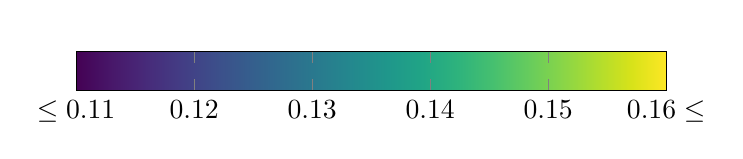
\begin{tikzpicture}
      \begin{axis}[
          hide axis,
          scale only axis,
          height=0pt,
          width=0pt,
          colormap/viridis,
          colorbar horizontal,
          point meta min=0.11,
          point meta max=0.16,
          colorbar style={
              %title= {$\abs{\rho_{01}}^2$},
              width=0.6180339887\textwidth,
              xtick={0.11, 0.12, 0.13, 0.14, 0.15, 0.16},
              xticklabels={$\le 0.11$, $0.12$, $0.13$, $0.14$, $0.15$, $0.16\le$}
          }]
          \addplot [draw=none] coordinates {(0,0)};
      \end{axis}
    \end{tikzpicture}
  } \\
  \subfloat{\includegraphics[width=\textwidth]{figures/tube/tube_print_0.png}} \\
  \subfloat{\includegraphics[width=\textwidth]{figures/tube/tube_print_1.png}} \\
  \subfloat{\includegraphics[width=\textwidth]{figures/tube/tube_print_2.png}} \\
  \subfloat{\includegraphics[width=\textwidth]{figures/tube/tube_print_3.png}} \\
  \caption{\label{fig:tubes}
    Coloration of $\abs{\tilde{\rho}_{01}}^2$ at $t_1 = \SI{-0.05}{\pico\second}$, $t_2 = \SI{0}{\pico\second}$, $t_3 = \SI{0.05}{\pico\second}$, and $t_4 = \SI{0.10}{\pico\second}$ relative to the peak of a \SI{1}{\pico\second}-wide $\pi$-pulse.
    \num{10000} \qds{} randomly distributed throughout a $\SI{0.2}{\micro\meter} \text{ (radius)} \times \SI{4}{\micro\meter}$ cylinder oriented along $\vb{k}_L$ demonstrate near-field the effects of \cref{fig:density stats} as distinct, outlying bright/dark \qds{}.
    Additionally, the size of the system allows for wavelengh-scale phenomena that appear here as five standing regions of enhanced polarization.
  }
  
\end{figure*}
\begin{figure}
  \centering
  \subfloat[\label{fig:polarization fluctuation}Projection of the cylinder in \cref{fig:tubes} at $t_3$ onto the cylindrical axis.]{\input{figures/z_polarization_distribution.tex}} \\
  \subfloat[\label{fig:end tubes}Projections of the cylinders in \cref{fig:tubes} onto the $xy$-plane.]{
    \includegraphics[width=0.24\linewidth]{figures/tube/end_print_0.png}
    \includegraphics[width=0.24\linewidth]{figures/tube/end_print_1.png}
    \includegraphics[width=0.24\linewidth]{figures/tube/end_print_2.png}
    \includegraphics[width=0.24\linewidth]{figures/tube/end_print_3.png}
  }
  \caption{\label{fig:tube projection}
    Polarization projections of the cylinders in \cref{fig:tubes}.
    The projection onto the cylindrical axis reveals the five standing nodes of polarization as well as a tendency for increased polarization near the ends of the cylinder.
    The uniform orientation of the dipole radiators breaks the cylindrical symmetry of the system, leading to radial anisotropies in the polarization intensity.
  }
\end{figure}

\section{Conclusions \& Future work}
Here we have presented a robust, fine-grained algorithm to solve for the dyanmics of a semiclassical ensemble of coupled \qds{} in response to an external laser pulse. 
By making use of an integral equation kernel to propagate radiated fields, our model eschews inefficient radiation meshes in favor of a more efficient point-to-point communication strategy, facillitating simulations of many thousands of \qds{} in three dimensions.
Our simulations predict very tightly coupled dynamics in dense \qd{} systems---these systems produce a number of clusters that evolve with frequencies not present in the incident field, and we have shown this behavior depends critically on the presence of many-body interactions.
Additionally, many \qds{} interact so as to screen out the majority of the incident field, thereby changing very little from their initial configuration.

Given prior work in this area, we predict superradiant and other similar phenomena will occcur in electrically large systems containing many millions of particles.
Unfortunately, the na\"ive $n^2$ calculation between every pair of \qds{} given here presents a significant computational bottleneck in trying to investigate these dynamics.
The primary focus of our ongoing research includes the development of an accelerated computational technique to reduce this cost so as to investigate these (and other similar) systems.
Additionally, the framework presented here readily extends to model \qds{} with richer structure (such as energy degeneracies or biexcitons)---systems we hope to investigate soon.

%\appendix
%\section{Derivation of \cref{eq:integral operator}}

For time-harmonic (monochromatic) electric fields, we require
\begin{equation}
  \vb{E}_\omega = - \frac{1}{c} \qty(i \omega \vb{A}_\omega) - \grad \phi_\omega
  \label{eq:potential e-field}
\end{equation}
where $G_\omega(\vb{r} - \vb{r}') = e^{i k \abs{\vb{r} - \vb{r}'}}/\abs{\vb{r} - \vb{r}'}$ and
\begin{subequations}
  \begin{align}
      \phi_\omega(\vb{r}) &= \int \! G(\vb{r} - \vb{r}') \rho_\omega(\vb{r}') \dd[3]{\vb{r}'} \label{eq:scalar potential} \\
    \vb{A}_\omega(\vb{r}) &= \frac{1}{c} \int \! G(\vb{r} - \vb{r}') \vb{J}_\omega(\vb{r}') \dd[3]{\vb{r}'}. \label{eq:vector potential}
  \end{align}
\end{subequations}
Choosing a Lorentz gauge, i.e.\
\begin{equation}
  \div{\vb{A}_\omega} + \frac{1}{c} \qty(i \omega \phi_\omega) = 0
\end{equation}
and inserting \cref{eq:vector potential}, we may rewrite \cref{eq:potential e-field} as
\begin{widetext}
\begin{equation}
  \vb{E}_\omega(\vb{r}) = -\frac{i \omega}{c^2} \int \! G_\omega(\vb{r} - \vb{r}') \vb{J}_\omega(\vb{r}') \dd[3]{\vb{r}'} + \frac{1}{i \omega} \grad \qty( \div \int \! G_\omega(\vb{r} - \vb{r}') \vb{J}_\omega(\vb{r}') \dd[3]{\vb{r}'} ).
  \label{eq:e in terms of j}
\end{equation}
\end{widetext}
As $\vb{r}$ does not lie within the source region, the derivatives commute with the integral in the second term of \cref{eq:e in terms of j}.
Noting that
\begin{equation}
  \div \qty\Big(G_\omega(\vb{r} - \vb{r}') \vb{J}_\omega(\vb{r}')) =\grad{G_\omega(\vb{r} - \vb{r}')} \cdot \vb{J}_\omega(\vb{r}')
\end{equation}
as $\vb{J}_\omega(\vb{r}')$ is not a function of $\vb{r}$, we may compactly write \cref{eq:e in terms of j} as
\begin{equation}
  \vb{E}_\omega(\vb{r}) = -\frac{i \omega}{c^2} \int \! \tensor{\mathrm{G}}_d(\vb{r} - \vb{r}') \cdot \vb{J}_\omega(\vb{r}') \dd[3]{\vb{r}'}
  \label{eq:frequency domain dyadic green function}
\end{equation}
where
\begin{equation}
  \tensor{\mathrm{G}}_d(\vb{r}) = \qty[\tensor{\mathrm{I}} + \frac{\grad \grad}{k^2}]G_\omega(\vb{r}).
\end{equation}
Recalling $\grad{\bar{\vb{r}}} = \qty(\tensor{\mathrm{I}} - \outerprod{\bar{\vb{r}}}{\bar{\vb{r}}})/r$,
\begin{equation}
  \begin{aligned}
    \tensor{\mathrm{G}}_d(\vb{r}) &= \qty(\tensor{\mathrm{I}} - \outerprod{\bar{\vb{r}}}{\bar{\vb{r}}}) G_\omega(\vb{r}) \\
                                  &- \qty(\frac{i}{k r} + \frac{1}{(k r)^2} ) \qty(\tensor{\mathrm{I}} - 3 \outerprod{\bar{\vb{r}}}{\bar{\vb{r}}}) G_\omega(\vb{r})
  \end{aligned}
\end{equation}


\bibliography{refs/random_lasing_reflist}

\end{document}
